\documentclass[11pt,oneside]{book}
\usepackage{fontspec}
\setmainfont{Noto Serif}
\setsansfont{Noto Sans}
\setmonofont{Noto Sans Mono}
\newfontfamily\proseunicodefont{DejaVu Serif}
\usepackage[margin=1in]{geometry}
\usepackage{microtype}
\usepackage{amsmath,amssymb,amsthm,mathtools,bm}
\usepackage{graphicx}
\usepackage{adjustbox}
\usepackage{xcolor}
\usepackage{booktabs}
\usepackage{array}
\usepackage{longtable}
\usepackage{enumitem}
\usepackage{float}
\usepackage{caption}
\usepackage{hyperref}
\usepackage{fancyhdr}
\usepackage{tikz}
\usetikzlibrary{arrows.meta,positioning,calc,decorations.pathmorphing}

\hypersetup{
  colorlinks=true,
  linkcolor=blue!50!black,
  urlcolor=blue!50!black,
  citecolor=blue!50!black
}

\setlength{\parskip}{0.5em}
\setlength{\parindent}{0pt}
\setlist[itemize]{topsep=0.25em,itemsep=0.2em}
\setlist[enumerate]{topsep=0.25em,itemsep=0.2em}
\setlength{\headheight}{40pt}
\numberwithin{equation}{chapter}

\newtheorem{theorem}{Teorema}[chapter]
\newtheorem{proposition}[theorem]{Proposición}
\newtheorem{lemma}[theorem]{Lema}
\newtheorem{corollary}[theorem]{Corolario}
\theoremstyle{definition}
\newtheorem{definition}[theorem]{Definición}
\newtheorem{example}[theorem]{Ejemplo}
\theoremstyle{remark}
\newtheorem{remark}[theorem]{Observación}

\providecommand{\ket}[1]{\left\lvert#1\right\rangle}
\providecommand{\bra}[1]{\left\langle#1\right\rvert}
\providecommand{\braket}[2]{\left\langle#1\,\middle|\,#2\right\rangle}
\providecommand{\expect}[1]{\left\langle#1\right\rangle}
\newcommand{\lectureoverview}[1]{\paragraph{Resumen.} #1}

\makeatletter
\newcommand{\course@headerfont}{\normalfont\small\itshape}
\newcommand{\course@pagefont}{\normalfont\small}
\newcommand{\course@headerraise}{14pt}
\newlength{\course@headerboxheight}
\setlength{\course@headerboxheight}{\dimexpr\headheight-\course@headerraise-9pt\relax}
\newcommand{\course@leftheadbox}[1]{%
  \raisebox{\course@headerraise}{%
    \parbox[t][\course@headerboxheight][t]{0.82\textwidth}{%
      \raggedright\course@headerfont\strut\MakeUppercase{#1}\strut%
    }%
  }%
}
\newcommand{\course@rightheadbox}[1]{%
  \raisebox{\course@headerraise}{%
    \parbox[t][\course@headerboxheight][t]{0.82\textwidth}{%
      \raggedleft\course@headerfont\strut\MakeUppercase{#1}\strut%
    }%
  }%
}
\renewcommand{\chaptermark}[1]{\markboth{\MakeUppercase{\chaptername\ \thechapter.\ #1}}{}}
\renewcommand{\sectionmark}[1]{\markright{\MakeUppercase{\thesection\hspace{0.4em}#1}}}
\fancyhf{}
\fancyhead[L]{\course@leftheadbox{\leftmark}}
\fancyhead[R]{\course@pagefont\thepage}
\renewcommand{\headrulewidth}{0.5pt}
\pagestyle{fancy}
\fancypagestyle{plain}{%
  \fancyhf{}
  \fancyhead[L]{\course@leftheadbox{\leftmark}}
  \fancyhead[R]{\course@pagefont\thepage}
  \renewcommand{\headrulewidth}{0.5pt}
}
\makeatother

% Video2Book editorial provenance macros
\newenvironment{classroomqa}{%
  \par\medskip\noindent\begin{minipage}{\linewidth}\small\hrule\medskip
}{%
  \medskip\hrule\end{minipage}\par\medskip
}
\newcommand{\audiencequestion}[1]{\noindent\textbf{Pregunta del público.} #1\par\smallskip}
\newcommand{\lecturerresponse}[1]{\noindent\textbf{Respuesta.} #1\par}
\newcommand{\lecturetimestamp}[1]{\footnote{Marca temporal: #1.}}
\newcommand{\lectureframe}[1]{\par\smallskip{\centering\footnotesize\itshape Fotograma de la clase: #1.\par}}
\newcommand{\editorialnote}[1]{\footnote{Aclaración editorial: #1}}

\usepackage{polyglossia}
\setdefaultlanguage{spanish}
\usepackage{sectsty}
\renewcommand{\contentsname}{Índice}
\renewcommand{\chaptername}{Capítulo}
\renewcommand{\figurename}{Figura}
\renewcommand{\tablename}{Tabla}
\renewcommand{\proofname}{Demostración}
\renewcommand{\bibname}{Bibliografía}
\sectionfont{\raggedright}
\subsectionfont{\raggedright}
\makeatletter
\renewcommand{\@pnumwidth}{2.2em}
\renewcommand{\@tocrmarg}{3.2em}
\makeatother
\usepackage{tocloft}
\renewcommand{\cftchapfont}{\small\bfseries}
\renewcommand{\cftchappagefont}{\small\bfseries}
\renewcommand{\cftsecfont}{\small}
\renewcommand{\cftsecpagefont}{\small}
\setlength{\cftsecnumwidth}{3em}
\renewcommand{\cftsubsecfont}{\small}
\renewcommand{\cftsubsecpagefont}{\small}
\setlength{\cftsubsecindent}{4.5em}
\setlength{\cftsubsecnumwidth}{4em}
\emergencystretch=6em
\pdfstringdefDisableCommands{\def\proseunicodefont{}}

\geometry{paperwidth=177.6mm,paperheight=252mm,left=16mm,right=16mm,
 top=18mm,bottom=18mm,includeheadfoot,headheight=28pt,headsep=7mm,footskip=9mm}
\usepackage{scrextend}
\changefontsizes[17pt]{12pt}
\raggedbottom
\renewenvironment{classroomqa}{\par\medskip\begingroup}{\par\endgroup\medskip}
\fancyhf{}
\setlength{\headwidth}{\textwidth}
\fancyhead[L]{\parbox{\textwidth}{\raggedright\fontsize{9}{11}\selectfont\nouppercase{\leftmark}}}
\fancyfoot[C]{\small\thepage}
\renewcommand{\headrulewidth}{0.3pt}
\fancypagestyle{plain}{\fancyhf{}\fancyfoot[C]{\small\thepage}\renewcommand{\headrulewidth}{0pt}}

\graphicspath{{../../../generated_course_notes/supplementary/advanced_quantum_mechanics/2013_fall/figures/}{../../../generated_course_notes/supplementary/advanced_quantum_mechanics/2013_fall/assets/}}
\begin{document}
\frontmatter
\hypersetup{pageanchor=false}
\begin{titlepage}
\hyphenpenalty=10000\exhyphenpenalty=10000
\thispagestyle{empty}
\begin{tikzpicture}[remember picture,overlay]
  \node[anchor=center,inner sep=0] at (current page.center) {%
    \includegraphics[height=\paperheight,keepaspectratio]{../../../generated_course_notes/supplementary/advanced_quantum_mechanics/2013_fall/assets/cover-art.png}%
  };
  \node[
    anchor=north west,
    align=left,
    text width=0.78\paperwidth,
    fill=white,
    fill opacity=0.9,
    rounded corners=8pt,
    inner xsep=10pt,
    inner ysep=8pt
  ] at ([xshift=0.08\paperwidth,yshift=-0.06\paperheight]current page.north west) {%
    {\fontsize{30}{33}\selectfont\bfseries\color{black!88} Mecánica cuántica avanzada\\[0.85em]}
    {\large\color{black!72} Edición en español / otoño de 2013}
  };
  \node[
    anchor=south west,
    align=left,
    text width=0.68\paperwidth,
    fill=white,
    fill opacity=0.82,
    text opacity=1,
    rounded corners=6pt,
    inner sep=12pt
  ] at ([xshift=0.08\paperwidth,yshift=0.08\paperheight]current page.south west) {%
    {\normalsize\color{black!78} Clases originales: Leonard Susskind\\[0.35em]}
    {\small\color{black!72} Edición complementaria: \href{https://lazying.art}{LazyingArt LLC} / \href{https://github.com/lachlanchen/Video2Book}{Video2Book}}
  };
\end{tikzpicture}
\mbox{}
\end{titlepage}
\hypersetup{pageanchor=true}

\clearpage
\chapter{Sobre estas notas}
Estas notas complementarias, editadas de forma independiente, siguen las clases de Leonard Susskind. Se reconstruyeron a partir de transcripciones automáticas, subtítulos y fotogramas seleccionados de la pizarra, y luego se cotejaron con el material de fuente disponible. No son un manuscrito original del profesor Susskind ni han sido revisadas ni avaladas por él.

La edición fue preparada por \href{https://lazying.art}{LazyingArt LLC} mediante el flujo de trabajo de código abierto \href{https://github.com/lachlanchen/Video2Book}{Video2Book}. Las transcripciones automáticas siguen disponibles por separado y pueden contener errores de reconocimiento. Las aclaraciones editoriales y las reconstrucciones no triviales se identifican en notas al pie.
\clearpage
\tableofcontents
\mainmatter
\chapter{Vectores de estado, evolución unitaria y simetría de traslación}
\providecommand{\ket}[1]{\left\lvert#1\right\rangle}
\providecommand{\bra}[1]{\left\langle#1\right\rvert}

Tras un receso de dos trimestres, conviene hacer un repaso rápido de mecánica cuántica. No se puede dedicar todo el trimestre a ello. El tema que sigue es la aplicación de la mecánica cuántica a los problemas para los que se desarrolló originalmente: los átomos, los electrones y las partículas relacionadas, y los fotones.

Primero se estudian los átomos. ¿Cómo pueden estudiarse antes que los electrones, si estos forman parte de aquellos? Al principio basta con estudiar la mecánica de los electrones necesaria para escribir las ecuaciones básicas del átomo de hidrógeno. Después se puede estudiar con más detalle el comportamiento de las partículas similares a los electrones. En todas estas aplicaciones, la simetría será una herramienta recurrente: cómo se representan las simetrías en mecánica cuántica y qué implican para un sistema.

\section{Estados, observables y ortogonalidad}

En mecánica clásica, un estado se representa mediante un punto del espacio de fases. En mecánica cuántica, se representa mediante un vector de un espacio vectorial complejo. Se trata de un vector abstracto, no de una flecha en el espacio tridimensional ordinario. Los vectores de estado se pueden sumar y multiplicar por números complejos, y el espacio que los contiene no tiene por qué tener una dimensión finita determinada.

La notación de Dirac escribe un vector de estado como un ket,
\begin{equation}
\ket{\psi},
\end{equation}
y le asocia un bra,
\begin{equation}
\bra{\psi}.
\end{equation}
Los bras y los kets se relacionan mediante la conjugación hermítica. Al combinar un bra y un ket se obtiene un producto interno,
\begin{equation}
\langle\phi|\psi\rangle,
\end{equation}
que, en general, es un número complejo.

Un observable es algo que se puede medir: la posición, el momento, la energía o cualquier otra magnitud medible. En mecánica cuántica, un observable se representa mediante un operador lineal hermítico \(A\),
\begin{equation}
A^\dagger=A.
\end{equation}
La hermiticidad es el análogo de la realidad para los operadores. En particular, los valores propios de un operador hermítico son reales.

Un vector propio de \(A\) satisface
\begin{equation}
A\ket{\alpha}=\alpha\ket{\alpha}.
\end{equation}
Los posibles valores propios son los resultados posibles de medir \(A\). Por ejemplo, si un observable solo puede dar \(1\), \(3\) o \(7\), esos números son sus valores propios. Sus vectores propios son los estados en los que el resultado es definido, no estadístico. En el estado \(\ket{\alpha}\), medir \(A\) da \(\alpha\) con certeza.

El producto interno expresa una importante relación lógica entre estados. Supongamos que hay una medición que permite distinguir \(\ket{\phi}\) de \(\ket{\psi}\) con certeza. Entonces los estados son ortogonales:
\begin{equation}
\langle\phi|\psi\rangle=0.
\end{equation}
La ortogonalidad significa que los estados se pueden distinguir físicamente sin ambigüedad. Para un estado normalizado,
\begin{equation}
\langle\psi|\psi\rangle=1.
\end{equation}

\section{Una partícula en la representación de posición}

Consideremos primero una partícula que se mueve en una recta. Su posición \(x\) es un observable. Para cada posición posible \(x_0\), hay un estado \(\ket{x_0}\) en el que una medición de la posición da \(x_0\) con certeza.

Los estados asociados a posiciones diferentes se pueden distinguir y, por tanto, son ortogonales:
\begin{equation}
x\neq x'
\quad\Longrightarrow\quad
\langle x'|x\rangle=0.
\end{equation}
Para un estado arbitrario \(\ket{\psi}\), su producto interno con un estado de posición define la función de onda:
\begin{equation}
\psi(x)=\langle x|\psi\rangle.
\end{equation}
Esta es la representación del vector de estado en la posición.

La función de onda no es una probabilidad. Puede ser positiva, negativa, imaginaria o plenamente compleja. La densidad de probabilidad de posición es
\begin{equation}
P(x)=\psi^*(x)\psi(x)=|\psi(x)|^2.
\end{equation}
El producto es no negativo, como debe ser una densidad de probabilidad. Para una función de onda normalizada,
\begin{equation}
\int_{-\infty}^{\infty}dx\,|\psi(x)|^2=1.
\end{equation}

En la representación de posición, el operador posición actúa mediante multiplicación:
\begin{equation}
(\hat x\psi)(x)=x\psi(x).
\end{equation}
Sus funciones propias son funciones idealizadas concentradas en un solo punto. Se describen formalmente mediante deltas de Dirac: picos muy estrechos centrados en el valor propio de posición. Para este repaso no hace falta su definición precisa en el sentido de las distribuciones.

En tres dimensiones, la posición tiene tres componentes, \(x\), \(y\) y \(z\), y un estado de posición representa un punto del espacio tridimensional. Dos estados de este tipo son ortogonales si los puntos difieren en al menos una coordenada. Por lo general, se mantendrá la notación unidimensional, dando por entendida la extensión correspondiente a tres dimensiones.

\section{Momento y estados de momento definido}

A cada componente de la posición le corresponde una componente del momento. En la representación de posición, el operador momento a lo largo del eje \(x\) es
\begin{equation}
\hat p_x=-i\hbar\frac{d}{dx}.
\end{equation}
Así, un operador hermítico abstracto también se puede interpretar concretamente como una operación sobre funciones de onda.

Un estado de momento definido \(p_0\) satisface la ecuación de valores propios
\begin{equation}
\hat p_x\psi_{p_0}(x)=p_0\psi_{p_0}(x).
\end{equation}
Al sustituir la forma diferencial de \(\hat p_x\) se obtiene
\begin{equation}
-i\hbar\frac{d\psi_{p_0}(x)}{dx}
=p_0\psi_{p_0}(x).
\end{equation}
La derivada de la función de onda es proporcional a la función misma, así que la solución tiene forma exponencial:
\begin{equation}
\psi_{p_0}(x)\propto
\exp\left(\frac{ip_0x}{\hbar}\right).
\end{equation}

\begin{classroomqa}
\lecturetimestamp{00:24:26}
\audiencequestion{¿Se cumple esta ecuación diferencial para cualquier función de onda?}
\lecturerresponse{No. Es la ecuación de valores propios de un estado de momento definido. La mayoría de las funciones de onda no la satisface; esta ecuación selecciona las funciones propias del momento.}
\end{classroomqa}

La diferencia entre los estados propios de posición y los de momento es clara. Una función propia de posición está concentrada en un punto. Una función propia de momento tiene
\begin{equation}
\left|\exp\left(\frac{ip_0x}{\hbar}\right)\right|^2=1.
\end{equation}
Por lo tanto, su módulo es constante en toda la recta. En este sentido idealizado, un momento definido implica una incertidumbre completa en la posición; del mismo modo, una posición definida implica una incertidumbre completa en el momento. Este es el caso extremo de la relación de incertidumbre entre posición--momento.

\begin{classroomqa}
\lecturetimestamp{00:26:36}
\audiencequestion{Si se sabe que el momento es \(p_0\), ¿por qué sigue habiendo una distribución de probabilidad?}
\lecturerresponse{La cantidad mostrada corresponde a una medición de posición, no a otra medición de momento. El momento y la posición son observables distintos. Para el estado idealizado de momento propio, el módulo de la amplitud de posición es constante en toda la recta. Las amplitudes de momento pertenecen a la representación de momento y se relacionan con la función de onda de posición mediante una transformada de Fourier.}
\end{classroomqa}

\begin{classroomqa}
\lecturetimestamp{00:28:02}
\audiencequestion{¿Cómo es la probabilidad de posición cuando la función de onda es una delta de Dirac?}
\lecturerresponse{Está concentrada en la posición especificada. El pico idealizado expresa certeza en la posición.}
\end{classroomqa}

\editorialnote{Los estados propios exactos de posición y de momento son estados generalizados. Una delta de Dirac y una onda plana no son funciones de onda ordinarias, normalizables y de cuadrado integrable en toda la recta, y el cuadrado literal de una delta no es una distribución ordinaria. Las afirmaciones anteriores se refieren a su localización idealizada y a su módulo constante.}

Formalmente, una función de onda se puede considerar un vector con una componente para cada valor de \(x\). Sin embargo, a diferencia de un vector columna ordinario de dimensión finita, tiene un continuo infinito de componentes.

\begin{classroomqa}
\lecturetimestamp{00:28:53}
\audiencequestion{¿Se representan los vectores de estado mediante vectores columna?}
\lecturerresponse{Se pueden representar así, pero resulta incómodo escribir una función de onda de posición como un vector columna ordinario porque \(x\) toma continuamente muchos valores. Formalmente, se puede considerar un vector columna continuo, cuyo bra correspondiente se interpreta como un vector fila continuo.}
\end{classroomqa}

\section{Evolución temporal y unitariedad}

¿Cómo cambia un estado con el tiempo? La evolución temporal es una transformación del espacio de estados. Sea \(U(t)\) la evolución durante un intervalo de tiempo transcurrido \(t\). Entonces
\begin{equation}
U(t)\ket{\psi(t_1)}=\ket{\psi(t_1+t)}.
\end{equation}
En particular,
\begin{equation}
\ket{\psi(t)}=U(t)\ket{\psi(0)},
\qquad
U(0)=\mathbf 1.
\end{equation}

La condición sobre \(U(t)\) se desprende de la conservación de la información. Si dos estados iniciales se pueden distinguir, la evolución temporal no debe borrar esa distinción. Los estados ortogonales deben seguir siendo ortogonales. Más en general, se conserva el producto interno entre dos estados cualesquiera:
\begin{equation}
\langle U(t)\phi|U(t)\psi\rangle
=\langle\phi|\psi\rangle.
\end{equation}
Como
\begin{equation}
\langle U(t)\phi|U(t)\psi\rangle
=\langle\phi|U^\dagger(t)U(t)|\psi\rangle,
\end{equation}
la conservación de todos los productos internos exige
\begin{equation}
U^\dagger(t)U(t)=\mathbf 1.
\end{equation}
Un operador que satisface esta ecuación es unitario.

\begin{classroomqa}
\lecturetimestamp{00:36:36}
\audiencequestion{¿Conservar todos los productos internos es una condición más fuerte que conservar únicamente la ortogonalidad?}
\lecturerresponse{Para las transformaciones lineales de estados que estamos considerando, conservar la ortogonalidad implica conservar los productos internos. Las rotaciones ordinarias ofrecen la analogía habitual: conservan la ortogonalidad y los productos escalares.}
\end{classroomqa}

\editorialnote{En rigor, conservar solo la ortogonalidad permite una reescala global no nula. La conservación de la normalización, que ya se exige para la evolución temporal física, elimina esa libertad y da lugar a la conservación de los productos internos.}

Los operadores unitarios no deben confundirse con los observables hermíticos. La posición y el momento son hermíticos, pero en general no son unitarios. Los valores propios de un operador unitario son fases, números de la forma \(e^{i\theta}\) que están sobre el círculo unidad.

\begin{classroomqa}
\lecturetimestamp{00:38:12}
\audiencequestion{¿Cuál es un ejemplo de transformación no unitaria?}
\lecturerresponse{Los operadores posición y momento son ejemplos: son observables hermíticos, pero no son unitarios. Un operador unitario tiene valores propios de módulo unidad; por tanto, sus valores propios son fases.}
\end{classroomqa}

\section{El hamiltoniano y la ecuación de Schr\"odinger}

Se supone que la evolución temporal es continua. Por tanto, en un intervalo muy corto \(\epsilon\), el operador de evolución debe ser próximo a la identidad:
\begin{equation}
U(\epsilon)=\mathbf 1+\epsilon G+\mathcal O(\epsilon^2).
\end{equation}
Usando la unitariedad,
\begin{align}
U^\dagger(\epsilon)U(\epsilon)
&=
\left(\mathbf 1+\epsilon G^\dagger\right)
\left(\mathbf 1+\epsilon G\right)
+\mathcal O(\epsilon^2)
\\
&=
\mathbf 1+\epsilon(G^\dagger+G)
+\mathcal O(\epsilon^2).
\end{align}
A primer orden,
\begin{equation}
G^\dagger=-G.
\end{equation}
Así, \(G\) es antihermítico. Se puede escribir como
\begin{equation}
G=-\frac{i}{\hbar}H,
\end{equation}
donde \(H\) es hermítico:
\begin{equation}
H^\dagger=H.
\end{equation}
Por consiguiente, el operador infinitesimal de evolución temporal es
\begin{equation}
U(\epsilon)
=
\mathbf 1-\frac{i\epsilon}{\hbar}H
+\mathcal O(\epsilon^2).
\end{equation}
El operador hermítico \(H\) es el hamiltoniano.

\begin{classroomqa}
\lecturetimestamp{00:45:48}
\audiencequestion{¿Qué permite ignorar el término \(\epsilon^2\)?}
\lecturerresponse{El cálculo se realiza de manera consistente hasta primer orden en \(\epsilon\). Un cálculo de segundo orden requeriría todos los términos de segundo orden, incluido el término proporcional a \(-\epsilon^2H^2/(2\hbar^2)\). La aproximación está en la expresión truncada de \(U(\epsilon)\), no en la hermiticidad de \(H\).}
\end{classroomqa}

Se puede construir un intervalo de tiempo finito a partir de muchos intervalos pequeños. Dividamos \(t\) en \(N\) pasos de longitud \(t/N\). Al repetir la transformación infinitesimal se obtiene
\begin{equation}
U(t)
=
\lim_{N\to\infty}
\left(
\mathbf 1-\frac{itH}{N\hbar}
\right)^N
=
\exp\left(-\frac{iHt}{\hbar}\right).
\end{equation}
La exponencial es la versión finita de la transformación infinitesimal.

Ahora evolucionemos un estado desde \(t\) hasta \(t+\epsilon\):
\begin{align}
\ket{\psi(t+\epsilon)}
&=
U(\epsilon)\ket{\psi(t)}
\\
&=
\left(
\mathbf 1-\frac{i\epsilon}{\hbar}H
\right)\ket{\psi(t)}
+\mathcal O(\epsilon^2).
\end{align}
Restando \(\ket{\psi(t)}\), dividiendo por \(\epsilon\) y tomando el límite, se obtiene
\begin{equation}
\frac{d}{dt}\ket{\psi(t)}
=
-\frac{i}{\hbar}H\ket{\psi(t)}.
\end{equation}
De manera equivalente,
\begin{equation}
i\hbar\frac{d}{dt}\ket{\psi(t)}
=
H\ket{\psi(t)}.
\end{equation}
Esta es la ecuación de Schr\"odinger dependiente del tiempo. En la representación de posición se convierte en
\begin{equation}
i\hbar\frac{\partial}{\partial t}\psi(x,t)
=
H\psi(x,t),
\end{equation}
donde \(H\) actúa como operador sobre la función de onda.

La ecuación de Schr\"odinger independiente del tiempo es la ecuación de valores propios del hamiltoniano:
\begin{equation}
H\ket{E}=E\ket{E}.
\end{equation}
Los valores propios \(E\) son las energías que se pueden medir, o niveles de energía. Por tanto, el mismo hamiltoniano determina tanto las energías permitidas como la evolución del estado.

Si el estado inicial es un estado propio de energía, su evolución es
\begin{equation}
\ket{E;t}
=
\exp\left(-\frac{iEt}{\hbar}\right)\ket{E}.
\end{equation}
Sigue siendo el mismo vector propio de energía y solo adquiere una fase.\footnote{El signo menos queda fijado por la derivación anterior de \(U(t)=\exp(-iHt/\hbar)\). Una formulación oral posterior de la fase lleva el signo opuesto y es incompatible con esa derivación.}

\begin{classroomqa}
\lecturetimestamp{01:01:05}
\audiencequestion{¿Cómo evoluciona un vector propio de energía según la ecuación de Schr\"odinger dependiente del tiempo?}
\lecturerresponse{Conservemos el ket. Dado que \(H\ket{E}=E\ket{E}\), la evolución temporal multiplica el vector propio de energía por una fase determinada por su energía: \(\exp(-iEt/\hbar)\).}
\end{classroomqa}

\section{¿Qué se considera una simetría?}

La evolución temporal es una transformación unitaria del espacio de estados. Las transformaciones de simetría constituyen otra clase importante.

La simetría de rotación es fundamental en la física atómica. En un átomo de hidrógeno, el electrón se mueve en el potencial central de Coulomb. Una rotación del sistema de coordenadas no cambia las ecuaciones y, al rotar físicamente el átomo, este sigue siendo un átomo de hidrógeno regido por las mismas ecuaciones. El estado puede cambiar con la rotación, pero la ley dinámica no cambia.

La traslación ofrece otro ejemplo. Un sistema aislado en el espacio vacío debería comportarse igual después de desplazar todas sus partes la misma distancia. Esta salvedad es importante. Si hay un horno y solo se acerca el sistema a él, el comportamiento del sistema puede cambiar; el horno rompe esa simetría de traslación. Si se trasladan juntos el sistema y el horno, se restablece la relación original entre ambos.

No toda operación es una simetría. Comprimir un cristal de sal gema a la mitad de su tamaño suele cambiar su comportamiento. La compresión es una transformación bien definida, pero en general no es una simetría.

Así pues, una simetría es una operación sobre los estados que conserva la forma de la dinámica. Denotémosla por \(V\). Debe conservar la distinguibilidad: dos estados ortogonales deben seguir siendo ortogonales después de la transformación. Por tanto,
\begin{equation}
V^\dagger V=\mathbf 1,
\end{equation}
de modo que \(V\) es unitario.

\section{Las simetrías conmutan con la evolución temporal}

Supongamos que un estado inicial \(\ket{\psi_1}\) evoluciona hasta \(\ket{\psi_2}\):
\begin{equation}
\ket{\psi_2}=U(t)\ket{\psi_1}.
\end{equation}
Apliquemos a ambos estados una simetría propuesta \(V\):
\begin{equation}
\ket{\psi_1'}=V\ket{\psi_1},
\qquad
\ket{\psi_2'}=V\ket{\psi_2}.
\end{equation}
Si \(V\) es una simetría de la dinámica, el estado inicial transformado debe evolucionar hasta el estado final transformado:
\begin{equation}
\ket{\psi_2'}=U(t)\ket{\psi_1'}.
\end{equation}
Al sustituir las definiciones se obtiene
\begin{equation}
VU(t)\ket{\psi_1}
=
U(t)V\ket{\psi_1}.
\end{equation}
Esto debe cumplirse para todo estado inicial. Por tanto,
\begin{equation}
VU(t)=U(t)V.
\end{equation}

Las dos vías equivalentes se pueden representar en un diagrama conmutativo.\footnote{El diagrama reconstruye el argumento de las dos vías desarrollado entre 01:10:30 y 01:16:34.}
\begin{figure}
\centering
\begin{tikzpicture}[>=Stealth]
\node (a) at (0,0) {$\ket{\psi_1}$};
\node (b) at (4.2,0) {$\ket{\psi_2}=U(t)\ket{\psi_1}$};
\node (c) at (0,-2.0) {$V\ket{\psi_1}$};
\node (d) at (4.2,-2.0) {$V\ket{\psi_2}=U(t)V\ket{\psi_1}$};

\draw[->] (a) -- node[above] {$U(t)$} (b);
\draw[->] (c) -- node[below] {$U(t)$} (d);
\draw[->] (a) -- node[left] {$V$} (c);
\draw[->] (b) -- node[right] {$V$} (d);
\end{tikzpicture}
\caption{Una operación de simetría y la evolución temporal conducen al mismo estado final, en cualquier orden.}
\end{figure}

\begin{classroomqa}
\lecturetimestamp{01:16:38}
\audiencequestion{¿Debe conmutar la simetría con la evolución temporal para cualquier tiempo?}
\lecturerresponse{Sí. Una simetría de la dinámica debe satisfacer la condición de conmutación para la evolución temporal completa.}
\end{classroomqa}

\begin{classroomqa}
\lecturetimestamp{01:17:13}
\audiencequestion{¿Significa esto que se puede rotar y luego esperar, o esperar y luego rotar?}
\lecturerresponse{Exactamente. Si la rotación es una simetría, ambos órdenes producen el mismo estado final transformado.}
\end{classroomqa}

Para un intervalo de tiempo pequeño,
\begin{equation}
U(\epsilon)
=
\mathbf 1-\frac{i\epsilon}{\hbar}H
+\mathcal O(\epsilon^2).
\end{equation}
La condición de conmutación se convierte en
\begin{equation}
V\left(
\mathbf 1-\frac{i\epsilon}{\hbar}H
\right)
=
\left(
\mathbf 1-\frac{i\epsilon}{\hbar}H
\right)V
+\mathcal O(\epsilon^2).
\end{equation}
Los términos de identidad se cancelan y queda
\begin{equation}
VH=HV,
\end{equation}
o bien
\begin{equation}
[V,H]=0.
\end{equation}
Por tanto, una operación unitaria es una simetría de la dinámica si y solo si conmuta con el hamiltoniano.

\begin{classroomqa}
\lecturetimestamp{01:19:29}
\audiencequestion{¿Por qué el operador de simetría \(V\) debe ser unitario?}
\lecturerresponse{Una simetría debe conservar las distinciones lógicas entre estados. No debe transformar dos estados ortogonales y mutuamente excluyentes en estados que ya no se puedan distinguir. La conservación de esas relaciones exige una transformación unitaria.}
\end{classroomqa}

Un operador sin dependencia explícita del tiempo que conmuta con \(H\) es una cantidad conservada. Esto relaciona simetría y conservación. En mecánica clásica, la relación se expresa mediante el teorema de Noether. En la formulación cuántica que estamos desarrollando, la prueba central es el conmutador con el hamiltoniano.

\section{Simetrías discretas y continuas}

Las simetrías pueden ser discretas o continuas. Una reflexión especular es discreta: intercambia la izquierda y la derecha, sin que haya una secuencia de reflexiones infinitesimales que conecte ambas. El intercambio de dos partículas idénticas es otra operación discreta. Voltear un objeto sin marcas y con dos caras ofrece un ejemplo del mismo tipo.

Las rotaciones son continuas. Una rotación de \(90^\circ\) se puede construir mediante muchas rotaciones pequeñas alrededor del mismo eje. Por la misma razón, las traslaciones espaciales son continuas: un desplazamiento finito se puede construir a partir de muchos desplazamientos diminutos.

Esta divisibilidad en transformaciones pequeñas da a las simetrías continuas una forma especial. Cerca de la identidad, escribamos
\begin{equation}
V(\epsilon)
=
\mathbf 1-i\epsilon G+\mathcal O(\epsilon^2),
\end{equation}
donde \(\epsilon\) parametriza la transformación. La unitariedad implica
\begin{equation}
G^\dagger=G.
\end{equation}
El operador hermítico \(G\) se denomina generador de la simetría.

Si la transformación es una simetría, entonces
\begin{equation}
[H,V(\epsilon)]=0.
\end{equation}
Al desarrollar a primer orden se obtiene
\begin{equation}
[H,G]=0.
\end{equation}
Por tanto, las simetrías continuas están generadas por operadores hermíticos que conmutan con el hamiltoniano. Esos generadores son cantidades conservadas.

Aquí, la palabra ``generada'' tiene un significado concreto. Una transformación finita se construye aplicando repetidamente la transformación infinitesimal, del mismo modo que la evolución temporal finita se construye a partir de muchos intervalos de tiempo breves.

\section{Simetría de traslación y momento}

Consideremos una traslación activa de una función de onda hacia la derecha una distancia \(\epsilon\). Si la función de onda original presenta un máximo en \(x_0\), la función trasladada debe presentarlo en \(x_0+\epsilon\). Por tanto, su valor en la coordenada \(x\) es el valor de la función de onda original evaluada en \(x-\epsilon\):
\begin{equation}
(T(\epsilon)\psi)(x)=\psi(x-\epsilon).
\end{equation}
Para un desplazamiento pequeño,
\begin{equation}
\psi(x-\epsilon)
=
\psi(x)-\epsilon\frac{d\psi(x)}{dx}
+\mathcal O(\epsilon^2).
\end{equation}
De ahí que
\begin{equation}
T(\epsilon)
=
\mathbf 1-\epsilon\frac{d}{dx}
+\mathcal O(\epsilon^2).
\end{equation}
Usando
\begin{equation}
\hat p_x=-i\hbar\frac{d}{dx},
\qquad
\frac{d}{dx}=\frac{i}{\hbar}\hat p_x,
\end{equation}
la traslación infinitesimal queda
\begin{equation}
T(\epsilon)
=
\mathbf 1-\frac{i\epsilon}{\hbar}\hat p_x
+\mathcal O(\epsilon^2).
\end{equation}
La traslación finita correspondiente es
\begin{equation}
T(\epsilon)
=
\exp\left(-\frac{i\epsilon}{\hbar}\hat p_x\right).
\end{equation}
Con la convención \(V(\epsilon)=\mathbf 1-i\epsilon G+\cdots\), el parámetro de traslación con dimensiones da
\begin{equation}
G_{\mathrm{trans}}=\frac{\hat p_x}{\hbar}.
\end{equation}
De manera equivalente, se dice que el momento es el generador de las traslaciones espaciales cuando se muestra el factor de \(\hbar\) en la exponencial.

\begin{classroomqa}
\lecturetimestamp{01:34:08}
\audiencequestion{¿Se perdió un signo menos en la derivación de la traslación?}
\lecturerresponse{La cuestión es qué dirección se asigna a la función de onda trasladada. Un desplazamiento activo hacia la derecha se representa mediante \(\psi(x-\epsilon)\), no mediante \(\psi(x+\epsilon)\). Con esa corrección, \(T(\epsilon)=\mathbf 1-i\epsilon\hat p_x/\hbar+\cdots\).}
\end{classroomqa}

Que el momento se conserve depende del hamiltoniano. Para una partícula libre que se mueve en una dimensión,
\begin{equation}
H=\frac{\hat p_x^2}{2m}.
\end{equation}
Como todo operador conmuta con cualquier función de sí mismo,
\begin{equation}
[H,\hat p_x]=0.
\end{equation}
Por tanto, el hamiltoniano de la partícula libre es invariante ante traslaciones y \(\hat p_x\) se conserva. Físicamente, la partícula se comporta igual cualquiera que sea la posición inicial que se elija. Trasladar la condición inicial simplemente traslada todo el movimiento.

En tres dimensiones,
\begin{equation}
H
=
\frac{\hat p_x^2+\hat p_y^2+\hat p_z^2}{2m}.
\end{equation}
Cada componente del momento conmuta con \(H\):
\begin{equation}
[H,\hat p_x]=[H,\hat p_y]=[H,\hat p_z]=0.
\end{equation}
Hay una simetría de traslación independiente en cada dirección espacial. El momento es tanto la cantidad conservada como el generador asociado a esas traslaciones.

El siguiente caso es la simetría de rotación. Las rotaciones son más complejas porque, en general, las rotaciones alrededor de ejes distintos no conmutan: una rotación de \(x\) seguida de una de \(y\) no equivale a hacerlas en el orden inverso. Esto conduce a generadores de simetría que no conmutan y a la estructura de grupo de las rotaciones.

\chapter{Simetría, degeneración y escaleras de momento angular}
\providecommand{\ket}[1]{\left\lvert#1\right\rangle}

\section{Simetrías y niveles de energía degenerados}

Una simetría es una operación que no cambia la descripción física de un sistema. No cambia el hamiltoniano, la ecuación de Schr\"odinger ni las energías posibles. Si un operador unitario \(S\) representa la operación, la invariancia significa
\begin{equation}
S H S^\dagger=H,
\end{equation}
o, de manera equivalente,
\begin{equation}
[S,H]=0.
\end{equation}

La traslación es un ejemplo. Si se desplaza un átomo de un lugar a otro, su energía no cambia. Esto se cumple para todos los estados atómicos, no solo para el estado fundamental. La rotación es otro ejemplo y será el tema principal de esta sección.

El intercambio de dos partículas idénticas también es una simetría. Llamar electrón uno y electrón dos a dos electrones, o Harry y Fred, no los hace distintos. Intercambiar las etiquetas no puede cambiar las propiedades del átomo.

Un cristal tiene una simetría de traslación adicional. Desplazar todo el cristal por el espacio es una traslación ordinaria. Sin embargo, en un cristal infinito, una traslación de una constante de red también devuelve la misma disposición física. De manera equivalente, los sitios de la red se pueden volver a etiquetar desplazando en una unidad el índice de cada sitio. Los bordes impiden que esta afirmación sea exacta para un cristal finito, pero constituye una buena simetría lejos de los extremos de un cristal muy largo.

La homogeneidad del espacio---el hecho de que toda posición sea como cualquier otra---es la simetría de traslación. La isotropía del espacio---el hecho de que toda dirección sea como cualquier otra---es la simetría de rotación.

La degeneración está relacionada con la simetría, pero no es lo mismo. Un nivel de energía es degenerado cuando más de un estado tiene exactamente esa energía. Para un hamiltoniano genérico con espectro discreto, que dos niveles no relacionados coincidan exactamente sería un accidente asombroso. Una coincidencia de una parte en \(10^{15}\) sigue sin ser una igualdad exacta. Por lo general, las degeneraciones exactas indican la presencia de una simetría.

A veces la simetría implica degeneración, pero no siempre. El primer ejemplo muestra tanto por qué puede hacerlo como por qué una sola simetría quizá no sea suficiente.

\section{Una partícula en una circunferencia}

Consideremos una cuenta obligada a moverse sobre un alambre circular. Su posición podría describirse mediante las coordenadas cartesianas \(x\) y \(y\), pero basta con una coordenada angular:
\begin{equation}
\psi=\psi(\theta).
\end{equation}
La densidad de probabilidad de posición sobre la circunferencia es \(\psi^*(\theta)\psi(\theta)\).

Una rotación activa en sentido antihorario de un ángulo pequeño \(\epsilon\) transforma
\begin{equation}
\psi(\theta)\longrightarrow\psi(\theta-\epsilon).
\end{equation}
Por lo tanto,
\begin{align}
\delta\psi(\theta)
&=\psi(\theta-\epsilon)-\psi(\theta)\\
&=-\epsilon\frac{d\psi}{d\theta}
+\mathcal O(\epsilon^2).
\end{align}

El operador
\begin{equation}
L_z=-i\hbar\frac{d}{d\theta}
\end{equation}
es hermítico en el espacio de funciones de onda periódicas. Es el análogo angular de
\begin{equation}
p_x=-i\hbar\frac{d}{dx}.
\end{equation}
El factor \(i\) es esencial para la hermiticidad. En términos de \(L_z\),
\begin{equation}
\delta\psi
=-\frac{i\epsilon}{\hbar}L_z\psi
+\mathcal O(\epsilon^2),
\end{equation}
por lo que el operador de rotación infinitesimal es
\begin{equation}
R(\epsilon)
=1-\frac{i\epsilon}{\hbar}L_z
+\mathcal O(\epsilon^2).
\end{equation}
Esto identifica \(L_z\) como el generador de rotaciones alrededor del eje perpendicular a la circunferencia.

\begin{classroomqa}
\lecturetimestamp{00:11:19}
\audiencequestion{¿No debería tener signo opuesto uno de los factores que contienen \(i\)?}
\lecturerresponse{Al comprobar los signos se obtiene la relación anterior. Con la convención \(\psi(\theta)\to\psi(\theta-\epsilon)\), la variación es \(-\epsilon\,d\psi/d\theta\), que es igual a \(-i\epsilon L_z\psi/\hbar\).}
\end{classroomqa}

Ahora hallemos los estados propios del momento angular:
\begin{equation}
L_z\psi=M\psi.
\end{equation}
Al sustituir el operador diferencial se obtiene
\begin{equation}
-i\hbar\frac{d\psi}{d\theta}=M\psi,
\end{equation}
cuyas soluciones tienen la forma
\begin{equation}
\psi(\theta)=C\exp\left(\frac{iM\theta}{\hbar}\right).
\end{equation}

Hay una condición adicional que no se presenta para el movimiento sobre una recta infinita. Los puntos \(\theta=0\) y \(\theta=2\pi\) son el mismo punto, así que una función de onda orbital univaluada debe satisfacer
\begin{equation}
\psi(\theta+2\pi)=\psi(\theta).
\end{equation}
Para la autofunción anterior, esto exige
\begin{equation}
\exp\left(\frac{2\pi iM}{\hbar}\right)=1.
\end{equation}
En consecuencia,
\begin{equation}
M=m\hbar,
\qquad
m\in\mathbb Z.
\end{equation}
Por tanto, los valores posibles del momento angular orbital sobre la circunferencia son
\begin{equation}
\ldots,-2\hbar,-\hbar,0,\hbar,2\hbar,\ldots.
\end{equation}

¿Debe tener un estado con momento angular \(m\hbar\) la misma energía que un estado con momento angular \(-m\hbar\)? Los valores positivo y negativo de \(m\) describen sentidos de circulación opuestos. La pregunta es si la simetría de rotación por sí sola exige que esos dos movimientos tengan la misma energía.

\begin{classroomqa}
\lecturetimestamp{00:22:51}
\audiencequestion{¿Usar \(\psi(\theta-\epsilon)\) significa que la partícula se mueve en sentido horario?}
\lecturerresponse{No. Esa convención solo fija qué dirección se considera el sentido positivo de rotación. Define los signos de la posición angular y del momento angular, pero no determina la dirección real en que se mueve la partícula.}
\end{classroomqa}

Un campo magnético perpendicular al plano de la circunferencia proporciona un contraejemplo. Puede desplazar en sentidos opuestos las energías asociadas a momentos angulares positivos y negativos y, por tanto, desdoblar el par. El signo del desplazamiento depende de las convenciones para la carga y la orientación, pero lo importante es el desdoblamiento.

Ese campo sigue preservando las rotaciones alrededor del eje perpendicular. Por tanto, demuestra que la simetría de rotación por sí sola no exige
\begin{equation}
E(m)=E(-m).
\end{equation}
Si no hay desdoblamiento, \(m=1\) y \(m=-1\) pueden formar un par degenerado, al igual que \(m=2\) y \(m=-2\). El estado \(m=0\) no tiene un compañero distinto de este tipo.

\section{Simetría de reflexión y el par \texorpdfstring{\(m,-m\)}{m, -m}}

Añadamos una simetría discreta de reflexión. Sea \(\mathcal M\) la reflexión respecto de un diámetro de la circunferencia:
\begin{equation}
(\mathcal M\psi)(\theta)=\psi(-\theta).
\end{equation}
Esta invierte el sentido de circulación:
\begin{equation}
\mathcal M\psi_m=\psi_{-m}.
\end{equation}

Si la reflexión es una simetría, entonces
\begin{equation}
[\mathcal M,H]=0.
\end{equation}
Supongamos que
\begin{equation}
H\ket{m}=E_m\ket{m}.
\end{equation}
Al aplicar \(\mathcal M\) se obtiene
\begin{align}
H\mathcal M\ket{m}
&=\mathcal M H\ket{m}\\
&=E_m\mathcal M\ket{m}.
\end{align}
Como \(\mathcal M\ket{m}\) es el estado con momento angular \(-m\hbar\),
\begin{equation}
E_{-m}=E_m.
\end{equation}
La simetría de rotación conserva el momento angular; la simetría de reflexión relaciona sus dos valores opuestos. Juntas exigen que el par sea degenerado.

\begin{classroomqa}
\lecturetimestamp{00:29:54}
\audiencequestion{Como los modos \(m\) y \(-m\) tienen la misma densidad de probabilidad, ¿eso basta para demostrar que sus energías son iguales?}
\lecturerresponse{No. Las funciones de onda \(e^{im\theta}\) y \(e^{-im\theta}\) son diferentes, aunque sus módulos al cuadrado coincidan. La ecuación de valores propios del momento angular depende de la función de onda, no solo de \(\psi^*\psi\). La mecánica cuántica requiere amplitudes, no solo probabilidades.}
\end{classroomqa}

El campo magnético preserva las rotaciones alrededor de su eje, pero rompe la reflexión utilizada antes.

\begin{classroomqa}
\lecturetimestamp{00:33:05}
\audiencequestion{¿La simetría de reflexión invierte el campo magnético?}
\lecturerresponse{Sí. Un campo magnético es un vector axial. Al reflejar un campo que apunta hacia el interior de la pizarra, se obtiene uno que apunta hacia el exterior. De manera equivalente, una espira de corriente y su imagen especular llevan corrientes en sentidos opuestos y producen campos con direcciones opuestas.}
\end{classroomqa}

La no conmutatividad de la rotación y la reflexión se ve directamente. Para una autofunción del momento angular,
\begin{align}
\mathcal M L_z\psi_m
&=m\hbar\,\psi_{-m},\\
L_z\mathcal M\psi_m
&=-m\hbar\,\psi_{-m}.
\end{align}
Así,
\begin{equation}
[\mathcal M,L_z]\psi_m
=2m\hbar\,\psi_{-m},
\end{equation}
que es distinto de cero si \(m\neq0\). Rotar y luego reflejar no es la misma operación que reflejar y luego rotar.

Cuando ambas transformaciones son simetrías, los dos operadores conmutan con \(H\), pero no conmutan entre sí. Ese es el patrón responsable de la degeneración.

\begin{classroomqa}
\lecturetimestamp{00:40:28}
\audiencequestion{¿Cualquier par de Heisenberg que no conmute, como \(x\) y \(p\), genera degeneraciones?}
\lecturerresponse{Por lo general, no. Los operadores también deben ser simetrías: deben conmutar con el hamiltoniano. Típicamente, la posición y el momento no se conservan ambos. Si ambos conmutaran con \(H\), su no conmutatividad implicaría degeneración.}
\end{classroomqa}

\section{Álgebras de conmutadores de las simetrías}

Supongamos que \(A\) y \(B\) son los generadores hermíticos de dos simetrías continuas:
\begin{equation}
[A,H]=0,
\qquad
[B,H]=0.
\end{equation}
Estas ecuaciones no exigen que \(A\) y \(B\) conmuten entre sí.

El conmutador \([A,B]\) es antihermítico, así que definamos un operador hermítico
\begin{equation}
C=i[A,B].
\end{equation}
Aquí los factores numéricos y un signo global son irrelevantes. Lo importante es que \(C\) también conmuta con el hamiltoniano. En efecto,
\begin{equation}
[AB,H]
=A[B,H]+[A,H]B=0,
\end{equation}
y, de manera análoga,
\begin{equation}
[BA,H]=0.
\end{equation}
Por tanto,
\begin{equation}
[C,H]
=i\bigl([AB,H]-[BA,H]\bigr)=0.
\end{equation}

El nuevo generador \(C\) puede ser independiente de \(A\) y \(B\), o quizá solo sea una combinación lineal de generadores ya conocidos. Si es nuevo, lo añadimos a la lista y calculamos más conmutadores. Este proceso puede continuar indefinidamente, pero a menudo se cierra tras un número finito de generadores: todos los conmutadores posteriores son combinaciones lineales de los que ya están en la lista. Ese sistema cerrado es un álgebra de conmutadores o álgebra de Lie.

Las transformaciones de simetría finitas forman un grupo. Sus generadores infinitesimales forman el álgebra de Lie asociada.

Las degeneraciones son importantes porque organizan los espectros. Si dos estados tienen la misma energía, uno no puede decaer al otro emitiendo un fotón que transporte la diferencia entre sus energías. En la espectroscopia atómica, la disposición y degeneración de los niveles determinan las líneas espectrales posibles. El mismo razonamiento se aplica a los hadrones excitados y sus transiciones.

\begin{classroomqa}
\lecturetimestamp{00:49:07}
\audiencequestion{¿Son estos conmutadores elementos del grupo de simetría?}
\lecturerresponse{Los operadores en cuestión son generadores. Los generadores y sus conmutadores forman un álgebra de conmutadores, o álgebra de Lie. Las operaciones de simetría finitas construidas a partir de los generadores son los elementos del grupo.}
\end{classroomqa}

Si todos los generadores de simetría conmutan entre sí, la simetría se llama abeliana. Si alguno de sus conmutadores no es cero, es no abeliana.

\begin{classroomqa}
\lecturetimestamp{00:50:25}
\audiencequestion{¿Cuál es la definición fundamental de un generador?}
\lecturerresponse{Tomemos una transformación unitaria de simetría muy cercana a la identidad y escribámosla como \(1-i\epsilon G/\hbar+\cdots\). El operador hermítico \(G\) es su generador. Al repetir la transformación infinitesimal correspondiente, se obtiene una transformación finita.}
\end{classroomqa}

\begin{classroomqa}
\lecturetimestamp{00:52:08}
\audiencequestion{¿Qué se entiende por álgebra de los generadores de simetría?}
\lecturerresponse{Es una colección de generadores que se pueden sumar, restar, multiplicar por números ordinarios y conmutar. En esta álgebra, el conmutador desempeña el papel de la multiplicación, y el cierre significa que estas operaciones no producen generadores ajenos a la colección.}
\end{classroomqa}

\section{Rotaciones alrededor de ejes distintos}

Las rotaciones ofrecen el ejemplo más importante de una simetría no abeliana. Una rotación alrededor del eje \(x\) seguida de otra alrededor del eje \(y\) no suele equivaler a efectuarlas en el orden inverso. La diferencia entre ambas está relacionada, a su vez, con una rotación alrededor del tercer eje.

\begin{classroomqa}
\lecturetimestamp{00:54:22}
\audiencequestion{¿Las rotaciones infinitesimales conmutan aunque las rotaciones finitas no lo hagan?}
\lecturerresponse{Difieren en segundo orden con respecto a los dos ángulos pequeños de rotación. Eso basta: una vez factorizados esos parámetros pequeños, los generadores mismos tienen un conmutador distinto de cero.}
\end{classroomqa}

Antes de calcular los conmutadores cuánticos, consideremos el cuadro clásico correspondiente. Tomemos una órbita planetaria circular cuyo momento angular es perpendicular al plano orbital. Al rotar toda la órbita alrededor del eje \(y\) se obtiene otra órbita permitida con exactamente la misma energía. Sin embargo, el vector momento angular tiene ahora una componente \(x\) distinta.

Así, la invariancia rotacional produce configuraciones de igual energía con componentes distintas del momento angular. En mecánica cuántica, esto se manifiesta como la no conmutatividad entre los generadores de rotaciones alrededor de ejes distintos.

\section{Momento angular en coordenadas cartesianas}

Consideremos primero una partícula que se mueve en el plano \(xy\), sin restringirla a una circunferencia. Bajo una pequeña rotación antihoraria,
\begin{equation}
\delta x=-\epsilon y,
\qquad
\delta y=\epsilon x.
\end{equation}
Para el estado rotado activamente, la función de onda transformada se evalúa en las coordenadas rotadas por el ángulo inverso:
\begin{equation}
\psi_\epsilon(x,y)
=\psi(x+\epsilon y,y-\epsilon x).
\end{equation}
Por consiguiente,
\begin{align}
\delta\psi
&=\epsilon\left(
y\frac{\partial}{\partial x}
-x\frac{\partial}{\partial y}
\right)\psi
+\mathcal O(\epsilon^2)\\
&=-\frac{i\epsilon}{\hbar}
\left(xp_y-yp_x\right)\psi
+\mathcal O(\epsilon^2).
\end{align}
Por tanto, el generador de las rotaciones alrededor del eje \(z\) es
\begin{equation}
L_z=xp_y-yp_x.
\end{equation}
Esta es la componente \(z\) del conocido vector clásico
\begin{equation}
\mathbf L=\mathbf r\times\mathbf p.
\end{equation}
No es solo el momento angular mecánico; en mecánica cuántica, es el operador que genera rotaciones de la función de onda.\footnote{La convención de rotación activa se elige para que concuerde con la transformación anterior \(\psi(\theta)\mapsto\psi(\theta-\epsilon)\) y con la identificación final \(L_z=xp_y-yp_x\), tras la duda intermedia sobre el signo en la derivación oral.}

Al permutar cíclicamente \(x\to y\to z\to x\) se obtienen las demás componentes.\footnote{Las fórmulas para \(L_x\) y \(L_y\) se reconstruyen aplicando a \(L_z=xp_y-yp_x\) la sustitución cíclica \(x\to y\to z\to x\), indicada explícitamente en la clase.}
\begin{align}
L_x&=yp_z-zp_y,\\
L_y&=zp_x-xp_z,\\
L_z&=xp_y-yp_x.
\end{align}

Para un sistema invariante ante rotaciones, estos operadores conmutan con el hamiltoniano:
\begin{equation}
[H,L_x]=[H,L_y]=[H,L_z]=0.
\end{equation}
Una partícula en un campo de fuerzas central es el ejemplo típico. Estas ecuaciones expresan la conservación del momento angular en forma cuántica.

\section{El álgebra de Lie del momento angular}

Las relaciones de conmutación canónicas son
\begin{align}
[x_i,x_j]&=0,\\
[p_i,p_j]&=0,\\
[x_i,p_j]&=i\hbar\,\delta_{ij}.
\end{align}
Las coordenadas conmutan con las componentes del momento correspondientes a otras direcciones. Así, por ejemplo, \(x\) conmuta con \(p_y\), mientras que \(x\) no conmuta con \(p_x\).

Calculemos ahora
\begin{equation}
[L_x,L_y]
=
[yp_z-zp_y,\;zp_x-xp_z].
\end{equation}
La mayoría de los términos se anulan. Las dos contribuciones distintas de cero son
\begin{align}
[yp_z,zp_x]&=-i\hbar\,yp_x,\\
[zp_y,xp_z]&=i\hbar\,xp_y.
\end{align}
Por lo tanto,
\begin{align}
[L_x,L_y]
&=i\hbar\left(xp_y-yp_x\right)\\
&=i\hbar L_z.
\end{align}
Al permutar cíclicamente las etiquetas de las coordenadas se obtiene
\begin{align}
[L_x,L_y]&=i\hbar L_z,\\
[L_y,L_z]&=i\hbar L_x,\\
[L_z,L_x]&=i\hbar L_y.
\end{align}

\begin{classroomqa}
\lecturetimestamp{01:14:50}
\audiencequestion{Cuando el conmutador da como resultado \(L_z\), ¿aún tenemos que demostrar que \(L_z\) no es una combinación lineal de \(L_x\) y \(L_y\)?}
\lecturerresponse{Sí. Hay que establecer esa independencia, no darla por supuesta. En este punto no se desarrolla una demostración algebraica directa.}
\end{classroomqa}

Los conmutadores mostrados se cierran sobre el espacio generado por \(L_x\), \(L_y\) y \(L_z\): una vez incluidas las tres, los conmutadores posteriores no producen ningún operador fuera de ese espacio. Este es el álgebra de Lie del momento angular. Junto con
\begin{equation}
[H,L_i]=0,
\qquad i=x,y,z,
\end{equation}
estas relaciones contienen información sustancial sobre el espectro de energía, sin necesidad de resolver directamente la ecuación de Schr\"odinger angular.

Se emplea una estrategia algebraica similar para el oscilador armónico cuántico, cuyos operadores de creación y aniquilación generan su espectro. Aquí, los operadores análogos cambiarán la componente \(z\) del momento angular, en vez de la energía.

Elegir el eje \(z\) es solo una elección de representación. No hay razón física para preferir \(z\) a \(x\) o \(y\), pero escoger una componente proporciona una base conveniente. Escribamos
\begin{equation}
L_z\ket{m}=m\hbar\ket{m}.
\end{equation}
La tarea consiste en determinar qué valores de \(m\) pueden aparecer y cómo se relacionan los estados con distintos valores de \(m\).

\begin{classroomqa}
\lecturetimestamp{01:24:02}
\audiencequestion{Al comparar esta construcción con la del oscilador armónico, ¿se refiere al oscilador armónico cuántico? No se trató en la clase anterior.}
\lecturerresponse{Sí, la comparación es con el oscilador cuántico. El argumento actual sobre el momento angular es autocontenido y no requiere conocer el oscilador. Más adelante, la analogía también puede verse en sentido inverso: el oscilador emplea un método algebraico similar.}
\end{classroomqa}

\section{Operadores de subida y bajada del momento angular}

Definamos
\begin{equation}
L_+=L_x+iL_y,
\qquad
L_-=L_x-iL_y.
\end{equation}
Las relaciones de conmutación del momento angular implican que
\begin{equation}
[L_z,L_+]=\hbar L_+,
\qquad
[L_z,L_-]=-\hbar L_-.
\end{equation}

Apliquemos la primera relación a un estado propio de \(L_z\):
\begin{align}
L_zL_+\ket{m}
&=\left(L_+L_z+[L_z,L_+]\right)\ket{m}\\
&=(m+1)\hbar\,L_+\ket{m}.
\end{align}
Si \(L_+\ket{m}=0\), es otro estado propio de \(L_z\), ahora con valor propio \((m+1)\hbar\). De manera análoga,
\begin{equation}
L_zL_-\ket{m}
=(m-1)\hbar\,L_-\ket{m}.
\end{equation}
Así, \(L_+\) aumenta \(m\) en una unidad y \(L_-\) lo disminuye en una unidad.

A partir de cualquier valor propio, el álgebra genera una sucesión cuyos términos difieren en números enteros. La sucesión puede continuar indefinidamente o terminar porque
\begin{equation}
L_+\ket{m_{\mathrm{top}}}=0
\end{equation}
en el extremo superior y
\begin{equation}
L_-\ket{m_{\mathrm{bottom}}}=0
\end{equation}
en el extremo inferior.

\begin{classroomqa}
\lecturetimestamp{01:35:11}
\audiencequestion{¿No exigía ya el argumento de la circunferencia que el momento angular fuera un entero?}
\lecturerresponse{Ese argumento demuestra que el momento angular orbital toma valores enteros cuando se representa mediante funciones de onda de posición univaluadas. El álgebra abstracta del momento angular da un resultado menos restrictivo: la escalera puede contener valores enteros o semienteros.}
\end{classroomqa}

Si una escalera termina, la invariancia rotacional relaciona sus dos extremos. Una rotación de \(180^\circ\) alrededor de un eje perpendicular al eje \(z\) transforma
\begin{equation}
L_z\longrightarrow-L_z.
\end{equation}
Por tanto, el espectro debe ser simétrico respecto de cero:
\begin{equation}
m_{\mathrm{bottom}}=-m_{\mathrm{top}}.
\end{equation}
Como los valores consecutivos difieren en una unidad, hay dos posibilidades. La escalera contiene enteros,
\begin{equation}
\ldots,-2,-1,0,1,2,\ldots,
\end{equation}
o semienteros,
\begin{equation}
\ldots,-\frac{5}{2},-\frac{3}{2},-\frac{1}{2},
\frac{1}{2},\frac{3}{2},\frac{5}{2},\ldots,
\end{equation}
y sus extremos corresponden a los valores en los que el operador de subida o el de bajada se anula.

El argumento de la función de onda univaluada sobre la circunferencia selecciona la posibilidad de valores enteros para el momento angular orbital,
\begin{equation}
\mathbf L=\mathbf r\times\mathbf p.
\end{equation}
La posibilidad de valores semienteros también es física y corresponde al momento angular de espín, que se tratará por separado.

Por último, los estados de la escalera tienen la misma energía si el hamiltoniano es invariante ante rotaciones. Supongamos que
\begin{equation}
H\ket{m}=E\ket{m}.
\end{equation}
Como cada componente \(L_i\) conmuta con \(H\), \(L_+\) y \(L_-\) también lo hacen. Por tanto,
\begin{align}
H L_+\ket{m}
&=L_+H\ket{m}\\
&=E L_+\ket{m}.
\end{align}
Siempre que \(L_+\ket{m}\neq0\), el estado elevado tiene la misma energía que el estado original. El mismo cálculo da
\begin{equation}
H L_-\ket{m}=E L_-\ket{m}.
\end{equation}
Así pues, los operadores de subida y bajada generan una familia de estados con distintos valores propios de \(L_z\), pero exactamente la misma energía. Esta es la conexión entre simetrías no conmutativas y degeneración que se ha desarrollado a lo largo de la clase.

\begin{classroomqa}
\lecturetimestamp{01:44:13}
\audiencequestion{¿Estos estados de la escalera están asociados a elegir ejes de rotación distintos?}
\lecturerresponse{Están relacionados mediante rotaciones. Los vectores propios de \(L_x\) o \(L_y\) son combinaciones lineales de los vectores propios elegidos de \(L_z\). Al rotar un estado, cambian sus componentes de momento angular, pero su energía permanece inalterada.}
\end{classroomqa}

La elección de \(L_+\) y \(L_-\) resulta conveniente porque estas combinaciones ponen de manifiesto la escalera. Este recurso se repite a lo largo de la mecánica cuántica: cuando un álgebra de conmutadores se cierra, los operadores de subida y bajada suelen organizar el espectro de valores propios.

\begin{classroomqa}
\lecturetimestamp{01:46:33}
\audiencequestion{¿Qué ocurre cuando \(L_+\) actúa sobre el estado máximo, y cómo se define el extremo superior?}
\lecturerresponse{Da cero. Esa es la definición del extremo superior de una escalera que termina. De igual manera, \(L_-\) da cero en el extremo inferior. Una escalera abstracta no tiene por qué terminar. Para los estados de momento angular atómico que estudiaremos más adelante, lo habitual es encontrar escaleras que sí terminan.}
\end{classroomqa}

El siguiente paso es desarrollar más esta estructura del momento angular y aplicarla a los átomos, incluido el hidrógeno. Los multipletes rotacionales obtenidos aquí explican parte del patrón de degeneración; aún queda por desarrollar estructura adicional.

\chapter{Multipletes de momento angular, movimiento radial y escalera del oscilador}

\section{Dependencia angular de la función de onda}

Una partícula en un campo de fuerza central tiene una coordenada radial y dos coordenadas angulares. Clásicamente,
\begin{equation}
\mathbf L=\mathbf r\times\mathbf p
\end{equation}
se conserva como vector. Su dirección determina el plano de la órbita, aunque esta no tiene por qué ser circular.

En mecánica cuántica, la partícula se describe mediante
\begin{equation}
\Psi=\Psi(r,\theta,\phi),
\end{equation}
y el momento angular está relacionado con la dependencia de esta función de onda respecto de los ángulos.

En dos dimensiones solo hay una componente del momento angular: el generador de las rotaciones alrededor del eje perpendicular al plano:
\begin{equation}
L_z=-i\hbar\frac{\partial}{\partial\theta}.
\end{equation}
Una autofunción con autovalor \(\hbar\ell\) satisface
\begin{equation}
-i\hbar\frac{\partial}{\partial\theta}\psi(r,\theta)
=\hbar\ell\,\psi(r,\theta).
\end{equation}
La coordenada \(r\) es un parámetro espectador en esta ecuación. La solución tiene la forma
\begin{equation}
\psi(r,\theta)=\chi(r)e^{i\ell\theta}.
\end{equation}
Para una función de onda orbital ordinaria de valor único, volver al mismo punto tras \(\theta\to\theta+2\pi\) exige que \(\ell\) sea un entero. El factor radial \(\chi(r)\) puede afectar a la energía, pero no afecta a este autovalor del momento angular.

El análogo tridimensional separa la dependencia radial de las funciones definidas sobre la esfera:
\begin{equation}
\Psi(r,\theta,\phi)=R(r)Y_{\ell m}(\theta,\phi).
\end{equation}
Las funciones \(Y_{\ell m}\) son armónicos esféricos. Aquí no necesitaremos sus fórmulas explícitas. Las rotaciones actúan sobre el factor angular, mientras que la función radial permanece inalterada.

\section{Multipletes de momento angular finitos}

Las componentes del momento angular satisfacen
\begin{equation}
\begin{aligned}
[L_x,L_y]&=i\hbar L_z,\\
[L_y,L_z]&=i\hbar L_x,\\
[L_z,L_x]&=i\hbar L_y.
\end{aligned}
\end{equation}
Elijamos autoestados de \(L_z\),
\begin{equation}
L_z|\ell,m\rangle=\hbar m\,|\ell,m\rangle,
\end{equation}
y definamos
\begin{equation}
L_\pm=L_x\pm iL_y.
\end{equation}
Los conmutadores
\begin{equation}
[L_z,L_\pm]=\pm\hbar L_\pm
\end{equation}
dan
\begin{align}
L_z\bigl(L_\pm|\ell,m\rangle\bigr)
&=\bigl(L_\pm L_z+[L_z,L_\pm]\bigr)|\ell,m\rangle \\
&=\hbar(m\pm1)L_\pm|\ell,m\rangle.
\end{align}
Así, \(L_+\) aumenta \(m\) en una unidad y \(L_-\) lo disminuye en una unidad, salvo que el vector resultante sea nulo.

En un multiplete finito hay un estado de valor máximo y otro de valor mínimo:
\begin{equation}
L_+|\ell,\ell\rangle=0,
\qquad
L_-|\ell,-\ell\rangle=0.
\end{equation}
Las direcciones \(+z\) y \(-z\) están relacionadas por una rotación, por lo que el espectro finito es simétrico respecto de cero. Por tanto, sus valores son
\begin{equation}
m=-\ell,-\ell+1,\ldots,\ell-1,\ell,
\end{equation}
y el número de estados es
\begin{equation}
2\ell+1.
\end{equation}
Como los valores vecinos difieren en una unidad, los extremos pueden ser enteros o semienteros. Los armónicos esféricos orbitales ordinarios realizan el caso entero; el álgebra abstracta del momento angular también admite multipletes semienteros.

\begin{classroomqa}
\lecturetimestamp{00:16:12}
\audiencequestion{¿Podría un multiplete de momento angular contener infinitos estados?}
\lecturerresponse{Es una posibilidad que se puede considerar, pero no hará falta aquí. En general, el momento angular aumenta la energía si se mantienen fijas las demás características del estado; por ello, los estados con momento angular infinito no son pertinentes al estudiar estados de energía finita.}
\end{classroomqa}

\section{\texorpdfstring{\(L^2\)}{El valor común de }}

El operador que mide el cuadrado de la magnitud del momento angular es
\begin{equation}
L^2=L_x^2+L_y^2+L_z^2.
\end{equation}
El producto ordenado de los operadores escalera es
\begin{align}
L_-L_+
&=(L_x-iL_y)(L_x+iL_y) \\
&=L_x^2+L_y^2+i[L_x,L_y] \\
&=L_x^2+L_y^2-\hbar L_z.
\end{align}
En consecuencia,
\begin{equation}
L^2=L_z^2+\hbar L_z+L_-L_+.
\end{equation}
Apliquemos esta identidad al estado de valor máximo. Como \(L_+|\ell,\ell\rangle=0\),
\begin{align}
L^2|\ell,\ell\rangle
&=\left(L_z^2+\hbar L_z+L_-L_+\right)|\ell,\ell\rangle \\
&=\hbar^2\left(\ell^2+\ell\right)|\ell,\ell\rangle,
\end{align}
y, por tanto,
\begin{equation}
L^2|\ell,\ell\rangle
=\hbar^2\ell(\ell+1)|\ell,\ell\rangle.
\end{equation}
El cuadrado de la magnitud no es \(\hbar^2\ell^2\). El término adicional se debe a la no conmutatividad de las componentes del momento angular.

Este mismo valor corresponde a todos los estados del multiplete, no solo al de valor máximo.

\begin{classroomqa}
\lecturetimestamp{00:26:08}
\audiencequestion{¿Qué demuestra exactamente el ejercicio sobre la igualdad del valor de \(L^2\) para los demás estados?}
\lecturerresponse{Demuestre que \(L^2\) conmuta con cada componente del momento angular y, por tanto, con \(L_-\). Luego, haga pasar \(L^2\) a través de \(L_-\): si el estado de valor máximo tiene autovalor \(\hbar^2\ell(\ell+1)\), el estado inmediatamente inferior tiene el mismo autovalor. Al repetir el argumento, ese valor se conserva a lo largo de toda la escalera.}
\end{classroomqa}

En efecto,
\begin{equation}
[L^2,L_i]=0,
\qquad i=x,y,z,
\end{equation}
por lo que
\begin{equation}
[L^2,L_\pm]=0.
\end{equation}
Por ejemplo,
\begin{align}
L^2\bigl(L_-|\ell,\ell\rangle\bigr)
&=L_-L^2|\ell,\ell\rangle \\
&=\hbar^2\ell(\ell+1)L_-|\ell,\ell\rangle.
\end{align}
Al continuar hacia abajo se obtiene
\begin{equation}
L^2|\ell,m\rangle
=\hbar^2\ell(\ell+1)|\ell,m\rangle
\end{equation}
para todo \(m=-\ell,\ldots,\ell\).

El orden inverso da una factorización equivalente:
\begin{align}
L_+L_-
&=(L_x+iL_y)(L_x-iL_y) \\
&=L_x^2+L_y^2-i[L_x,L_y] \\
&=L_x^2+L_y^2+\hbar L_z,
\end{align}
y, por tanto,
\begin{equation}
L^2=L_z^2-\hbar L_z+L_+L_-.
\end{equation}

\begin{classroomqa}
\lecturetimestamp{00:32:05}
\audiencequestion{¿Se puede factorizar \(L_x^2+L_y^2\) en el orden inverso usando \(L_+L_-\)?}
\lecturerresponse{Sí. El signo del término \(L_z\) cambia. Con ese orden, aplique la identidad al estado de valor mínimo, que es anulado por \(L_-\), en vez de aplicarla al estado de valor máximo. Se obtiene el mismo autovalor, \(\hbar^2\ell(\ell+1)\).}
\end{classroomqa}

Por tanto, los armónicos esféricos satisfacen
\begin{align}
L^2Y_{\ell m}
&=\hbar^2\ell(\ell+1)Y_{\ell m}, \\
L_zY_{\ell m}
&=\hbar m\,Y_{\ell m}.
\end{align}
Para cada valor orbital \(\ell=0,1,2,\ldots\), hay \(2\ell+1\) funciones, etiquetadas por \(m=-\ell,\ldots,\ell\).

Para un potencial central,
\begin{equation}
[H,L_i]=0.
\end{equation}
Si se mantienen fijos un autoestado de energía radial y \(\ell\), cambiar \(m\) mediante \(L_\pm\) no modifica la energía. Por tanto, cada uno de esos autoestados radiales genera un multiplete magnético de dimensión \(2\ell+1\).

A continuación se muestra la escalera orbital entera.\footnote{El diagrama se reconstruyó a partir del esquema del multiplete y de las identidades de los operadores que aparecen en \(00{:}35{:}53\) del video de la clase.}

\begin{figure}[htbp]
\centering
\begin{tikzpicture}[x=1cm,y=0.85cm,>=stealth]
\draw[->] (0,-3.5) -- (0,3.5) node[above] {$m$};

\fill (0,3) circle (2.2pt);
\fill (0,2) circle (2.2pt);
\fill (0,0) circle (2.2pt);
\fill (0,-2) circle (2.2pt);
\fill (0,-3) circle (2.2pt);

\node[left] at (0,3) {$\ell$};
\node[left] at (0,2) {$\ell-1$};
\node[left] at (0,0) {$0$};
\node[left] at (0,-2) {$-\ell+1$};
\node[left] at (0,-3) {$-\ell$};

\node at (0,1) {$\vdots$};
\node at (0,-1) {$\vdots$};

\draw[->] (-1.15,-2.65) -- (-1.15,2.65)
node[midway,left] {$L_+$};
\draw[->] (1.15,2.65) -- (1.15,-2.65)
node[midway,right] {$L_-$};

\node[anchor=west] at (2.1,1.35)
{$L_z|\ell,m\rangle=\hbar m|\ell,m\rangle$};
\node[anchor=west] at (2.1,0.25)
{$L^2|\ell,m\rangle=\hbar^2\ell(\ell+1)|\ell,m\rangle$};
\node[anchor=west] at (2.1,-0.85)
{$L_\pm|\ell,m\rangle\propto|\ell,m\pm1\rangle$};
\end{tikzpicture}
\caption{Un multiplete entero de momento angular orbital. \(L_+\) y \(L_-\) cambian \(m\) en una unidad, mientras que \(L^2\) se mantiene igual a \(\hbar^2\ell(\ell+1)\) en todo el multiplete.}
\lectureframe{00:35:53}
\end{figure}

\section{El problema de la fuerza central}

Consideremos
\begin{equation}
H=\frac{\mathbf p^2}{2m}+V(r),
\end{equation}
donde \(V\) depende únicamente de la distancia al origen. La simetría rotacional implica la conservación del momento angular. Clásicamente, \(\mathbf L\) tiene magnitud y dirección fijas, de modo que la órbita permanece en un plano perpendicular a \(\mathbf L\). La órbita no tiene por qué ser circular ni siquiera cerrada.

Elijamos las coordenadas de modo que ese plano orbital clásico sea el plano \(xy\), y descompongamos el momento en sus componentes radial y tangencial:
\begin{equation}
\mathbf p^2=p_r^2+p_\theta^2.
\end{equation}
Como la magnitud del momento angular es
\begin{equation}
L=r p_\theta,
\end{equation}
la contribución tangencial se puede escribir como
\begin{equation}
p_\theta^2=\frac{L^2}{r^2}.
\end{equation}
El hamiltoniano queda
\begin{equation}
H=\frac{p_r^2}{2m}+\frac{L^2}{2mr^2}+V(r).
\end{equation}
Para un valor fijo de \(L\), este es un problema unidimensional en la coordenada radial, con potencial efectivo
\begin{equation}
V_{\mathrm{eff}}(r)=\frac{L^2}{2mr^2}+V(r).
\end{equation}
A continuación se muestra en la pizarra el hamiltoniano radial.\footnote{Fotograma de referencia: \texttt{\detokenize{lecture_03_frame_02.png}}, video de la clase en \(00{:}47{:}15\).}

\begin{figure}[htbp]
\centering
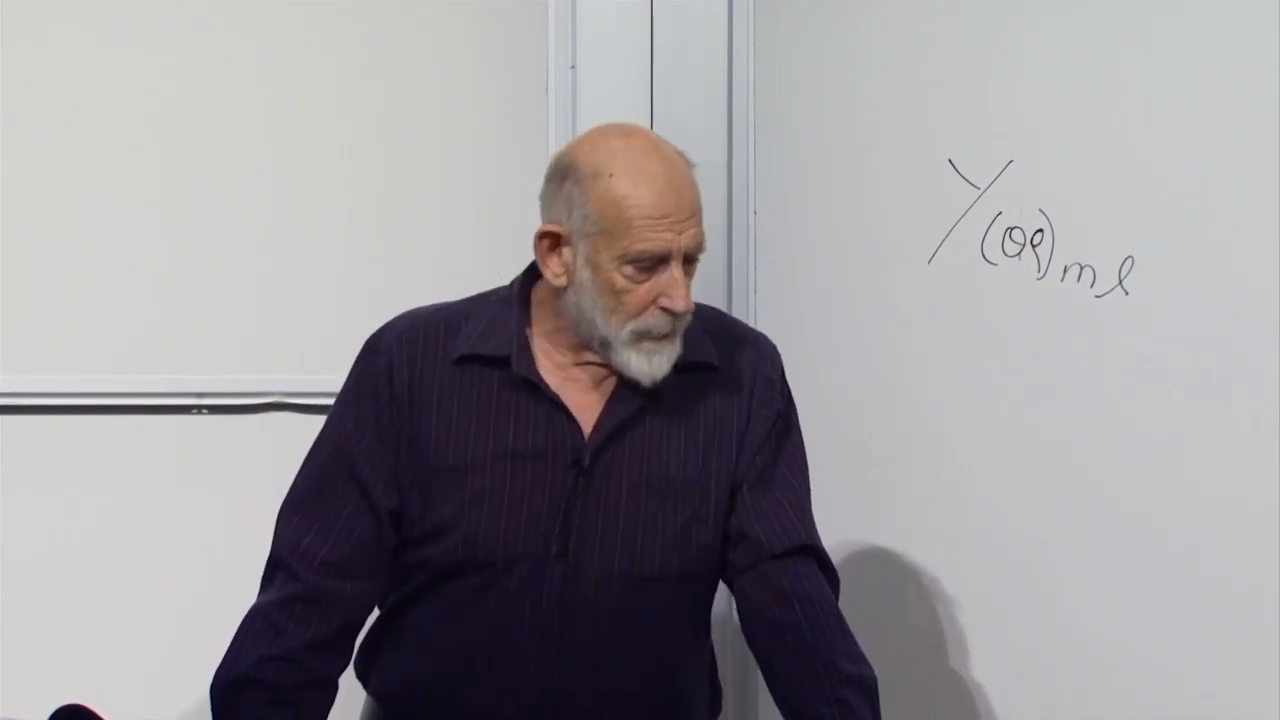
\includegraphics[width=0.9\linewidth]{lecture_03_frame_02.png}
\caption{Para un momento angular clásico fijo, el hamiltoniano radial contiene la energía cinética radial, el término centrífugo \(L^2/(2mr^2)\) y el potencial central \(V(r)\).}
\lectureframe{00:47:15}
\end{figure}

El término \(1/r^2\) es la barrera centrífuga. Aumenta cuando la partícula se acerca al origen, por lo que la fuerza asociada apunta hacia afuera. Para las atracciones de tipo Coulomb que estamos tratando, una trayectoria con \(L\neq0\) gira alrededor del centro en vez de llegar a él. Cuando \(L=0\), la barrera desaparece.

Para el potencial de Coulomb atractivo,
\begin{equation}
V(r)=-\frac{\kappa}{r},
\end{equation}
el término centrífugo domina a distancias pequeñas \(r\), mientras que el término de Coulomb decrece más lentamente y domina a distancias grandes \(r\). Si \(L\neq0\), la suma tiene un mínimo. El movimiento en ese mínimo tiene radio constante y, por tanto, es circular. El movimiento ligado por encima del mínimo y por debajo del umbral de escape oscila entre un radio mínimo y uno máximo; en el problema de Coulomb, estas son las oscilaciones radiales de una órbita elíptica.

\section{La ecuación radial reducida}

En mecánica cuántica, la parte angular de un estado con momento angular orbital definido es un armónico esférico. Escribamos el estado separado como
\begin{equation}
\Psi_{n_r\ell m}(r,\theta,\phi)
=\frac{u_{n_r\ell}(r)}{r}\,
Y_{\ell m}(\theta,\phi).
\end{equation}
El operador angular \(L^2\) tiene el autovalor
\begin{equation}
L^2Y_{\ell m}
=\hbar^2\ell(\ell+1)Y_{\ell m}.
\end{equation}
Para un par fijo \(n_r,\ell\), abreviemos \(u_{n_r\ell}(r)\) como \(u(r)\). La ecuación que queda para la función radial reducida es
\begin{equation}
\begin{aligned}
&-\frac{\hbar^2}{2m}\frac{d^2u}{dr^2}
+\frac{\hbar^2\ell(\ell+1)}{2mr^2}u(r)\\
&\qquad+V(r)u(r)=E_{n_r\ell}\,u(r).
\end{aligned}
\end{equation}

\editorialnote{\(u=rR\) es la función radial reducida que se utiliza en la ecuación unidimensional de derivadas segundas pura. Así, el término \(\psi(r)\) de la ecuación mostrada en la clase corresponde a \(u(r)\), mientras que el factor radial ordinario en \(\Psi=R(r)Y_{\ell m}\) es \(R=u/r\). Esta convención evita tratar \(-i\hbar\,d/dr\) como un operador de momento radial hermítico por sí solo en el espacio de Hilbert radial tridimensional.}

A continuación se muestra en la pizarra la ecuación radial reducida.\footnote{Fotograma de referencia: \texttt{\detokenize{lecture_03_frame_03.png}}, video de la clase en \(00{:}54{:}32\).}

\begin{figure}[htbp]
\centering
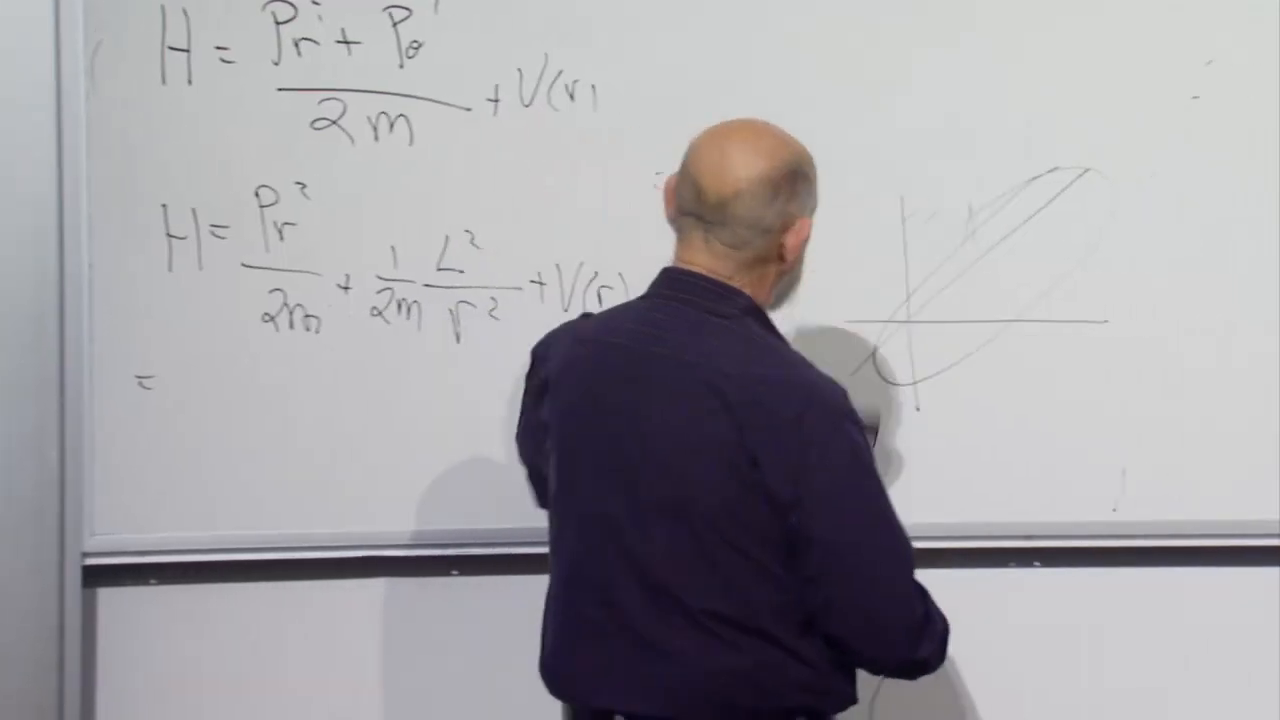
\includegraphics[width=0.9\linewidth]{lecture_03_frame_03.png}
\caption{Para un valor fijo de \(\ell\), la función de onda radial reducida satisface una ecuación unidimensional de Schr\"odinger con un término centrífugo proporcional a \(\ell(\ell+1)/r^2\).}
\lectureframe{00:54:32}
\end{figure}

La estructura angular tridimensional queda condensada en el parámetro \(\ell\). El número cuántico magnético \(m\) no aparece en la ecuación radial.

\begin{classroomqa}
\lecturetimestamp{00:55:34}
\audiencequestion{Para un valor dado de \(\ell\), ¿tienen la misma energía los \(2\ell+1\) estados magnéticos?}
\lecturerresponse{Sí, siempre que también se mantenga fijo el autoestado radial. Para cada valor elegido de \(u_{n_r\ell}\), todos los valores \(m=-\ell,\ldots,\ell\) tienen la misma energía porque \(m\) no aparece en la ecuación radial. En general, autoestados radiales distintos con el mismo \(\ell\) tienen energías diferentes.}
\end{classroomqa}

\begin{classroomqa}
\lecturetimestamp{00:56:03}
\audiencequestion{¿Por qué se puede sustituir \(L^2\) por \(\hbar^2\ell(\ell+1)\), y cómo se relaciona \(\ell\) con los valores permitidos de \(m\)?}
\lecturerresponse{El número \(\ell\) etiqueta un multiplete de momento angular y es el valor máximo de \(m\). Todos los estados de ese multiplete tienen el mismo autovalor de \(L^2\), \(\hbar^2\ell(\ell+1)\), y por eso se sustituye por ese autovalor en la ecuación radial.}
\end{classroomqa}

No hacen falta las soluciones explícitas en términos de funciones especiales para el argumento actual. Lo que importa es cómo se organizan las soluciones.

\section{Nodos radiales y niveles de energía}

Para un valor fijo de \(\ell\), la ecuación radial reducida es un problema unidimensional ordinario de autovalores. Sus estados ligados se ordenan según el número de nodos interiores. El estado radial más bajo no tiene nodos interiores; el siguiente tiene uno, y el que le sigue, dos. Cuantos más nodos, más rápidamente varía la función de onda; una variación más rápida implica mayor momento y, por tanto, mayor energía cinética.

Cada valor de \(\ell\) define un operador radial distinto, porque el término centrífugo cambia con \(\ell\). Así, los valores \(\ell=0,1,2,\ldots\) dan lugar a escaleras radiales separadas. El término centrífugo positivo desplaza los niveles hacia arriba al aumentar el momento angular. Cada autovalor radial con \(\ell\) fijo forma parte de un multiplete magnético de dimensión
\begin{equation}
2\ell+1.
\end{equation}
Los niveles \(\ell=0\) son singletes, los niveles \(\ell=1\) son tripletes y los niveles \(\ell=2\) son quintupletes. Estas son las degeneraciones garantizadas por la simetría rotacional; una simetría adicional también puede hacer degenerados estados con distintos valores de \(\ell\).

Para potenciales de tipo atómico que satisfacen \(V(r)\to0\) a grandes distancias \(r\), el umbral de escape se toma convencionalmente como \(E=0\). Los estados de energía negativa forman el espectro discreto de estados ligados. En \(E=0\) y por encima de ese valor aparece el continuo de dispersión. Esta afirmación depende del comportamiento del potencial a grandes distancias \(r\) y no se aplica a un potencial central confinante.

\section{La degeneración especial de Coulomb}

El potencial de Coulomb no relativista exacto presenta una alineación adicional de niveles. El estado radial más bajo con \(\ell=1\) tiene la misma energía que el primer estado excitado con \(\ell=0\). El siguiente estado con \(\ell=1\) se alinea con el segundo estado excitado con \(\ell=0\), y el estado más bajo con \(\ell=2\) se suma a ellos. El patrón continúa en las escaleras radiales y de momento angular más altas.

\begin{classroomqa}
\lecturetimestamp{01:09:57}
\audiencequestion{¿Esta degeneración adicional indica que existe otra simetría?}
\lecturerresponse{Sí. Es una simetría adicional inusual del potencial de Coulomb exacto. Pequeñas variaciones del potencial destruyen esta alineación, y aquí no se aborda su derivación.}
\end{classroomqa}

Las degeneraciones resultantes de las capas orbitales son
\begin{equation}
1,\qquad 4,\qquad 9,\qquad 16,\qquad \ldots
\end{equation}
antes de incluir el espín del electrón.

\begin{classroomqa}
\lecturetimestamp{01:11:46}
\audiencequestion{¿Esta degeneración describe el hidrógeno o solo el problema ideal de Coulomb?}
\lecturerresponse{El hidrógeno la cumple con muy buena aproximación, pero no exactamente. Las correcciones relativistas y el tamaño finito del núcleo alteran el patrón ideal de Coulomb.}
\end{classroomqa}

Un núcleo puntual produce un potencial exacto \(1/r\). Un núcleo cuya carga está distribuida en un volumen pequeño produce un potencial ligeramente distinto cuando el electrón penetra en ese volumen; incluso esta pequeña desviación elimina parte de la degeneración especial.

También se ha omitido el espín. Al incluir los dos estados de espín del electrón, el número de estados de cada capa se duplica y queda
\begin{equation}
2,\qquad 8,\qquad 18,\qquad 32,\qquad \ldots
\end{equation}
antes de resolver las desdoblamientos adicionales de un tratamiento atómico más completo.

\section{Revisión de la ecuación cartesiana}

La ecuación de partida del problema radial es la ecuación tridimensional de Schr\"odinger independiente del tiempo:
\begin{equation}
\begin{aligned}
-\frac{\hbar^2}{2m}\nabla^2\Psi+V(r)\Psi&=E\Psi,\\
\nabla^2&=\frac{\partial^2}{\partial x^2}
+\frac{\partial^2}{\partial y^2}
+\frac{\partial^2}{\partial z^2},\\
r&=\sqrt{x^2+y^2+z^2}.
\end{aligned}
\end{equation}
Pasemos a coordenadas radiales y angulares y seleccionemos un autoestado de \(L^2\).
Al sustituir \(L^2\) por \(\hbar^2\ell(\ell+1)\), la ecuación diferencial en derivadas parciales se reduce a la ecuación radial ordinaria anterior.

\begin{classroomqa}
\lecturetimestamp{01:16:42}
\audiencequestion{¿Se podrían usar las desviaciones respecto del espectro de Coulomb ideal para determinar el tamaño del núcleo?}
\lecturerresponse{No mediante esta comparación sencilla. Otras correcciones son mucho mayores y primero hay que tenerlas en cuenta. Se menciona aquí el tamaño nuclear porque ofrece un ejemplo inmediato de desviación respecto del potencial de Coulomb de una carga puntual.}
\end{classroomqa}

\begin{classroomqa}
\lecturetimestamp{01:17:09}
\audiencequestion{¿Cuál es la diferencia principal entre los términos de momento angular clásico y cuántico?}
\lecturerresponse{Clásicamente, \(L^2\) es el cuadrado ordinario de la magnitud de un vector conservado. En un multiplete orbital cuántico, su autovalor es \(\hbar^2\ell(\ell+1)\), no simplemente \(\hbar^2\ell^2\). El término adicional se debe a la no conmutatividad de las componentes del momento angular.}
\end{classroomqa}

\begin{classroomqa}
\lecturetimestamp{01:17:58}
\audiencequestion{¿Las funciones de onda de los estados ligados tienen soporte compacto?}
\lecturerresponse{No. Se extienden a distancias arbitrariamente grandes del centro. Para los estados ligados atómicos que estamos considerando, decrecen exponencialmente a grandes distancias; así, la probabilidad se vuelve despreciable, pero no se anula más allá de ningún radio finito.}
\end{classroomqa}

\begin{classroomqa}
\lecturetimestamp{01:18:48}
\audiencequestion{Cuando \(\ell=0\) elimina el pozo centrífugo, ¿qué ocurre con el punto estable?}
\lecturerresponse{Ya no hay un mínimo producido por la competencia entre la barrera centrífuga y la atracción. En la idealización de Coulomb puntual, el movimiento clásico se dirige hacia el centro singular. En mecánica cuántica, el estado más bajo no puede tener simultáneamente una posición exactamente definida en el centro y momento nulo, por lo que su función de onda tiene una extensión espacial finita.}
\end{classroomqa}

\editorialnote{Para un potencial central regular, una trayectoria clásica con momento angular nulo puede continuar a través del origen. En cambio, para el potencial ideal de Coulomb puntual, \(r=0\) es una singularidad de colisión, y la continuación de la trayectoria clásica requiere una prescripción adicional.}

La reducción clásica situó una órbita en un solo plano, pero ese paso no puede aplicarse del mismo modo a una función de onda cuántica. Un estado orbital cuántico ocupa el espacio tridimensional. El operador angular completo es \(L^2=L_x^2+L_y^2+L_z^2\), y su autovalor conserva el resultado tridimensional \(\hbar^2\ell(\ell+1)\).

\begin{classroomqa}
\lecturetimestamp{01:21:30}
\audiencequestion{¿Cómo puede el problema cuántico seguir siendo tridimensional si la órbita clásica se situó en un plano?}
\lecturerresponse{Solo se situó la órbita clásica en un plano fijo al elegir coordenadas perpendiculares a su vector de momento angular conservado. Una función de onda cuántica ocupa el espacio tridimensional. Las demás componentes del momento angular siguen presentes a través de \(L^2\), por eso la ecuación radial contiene \(\ell(\ell+1)\) en vez de solo el cuadrado de una componente.}
\end{classroomqa}

\begin{classroomqa}
\lecturetimestamp{01:22:54}
\audiencequestion{¿Todo problema cuántico admite operadores de subida y bajada?}
\lecturerresponse{No. Aparecen en casos especialmente favorables. El momento angular es uno de ellos, y el oscilador armónico es otro. El caso del oscilador es particularmente útil porque el movimiento cerca de un equilibrio estable suele ser aproximadamente armónico, incluidas las pequeñas oscilaciones radiales cerca del mínimo de un potencial efectivo.}
\end{classroomqa}

En este punto se deja de lado el problema atómico, y el oscilador armónico pasa a ser el siguiente ejemplo de un espectro determinado mediante operadores escalera.

\section{Pequeñas oscilaciones y el oscilador armónico}

Cerca de un equilibrio estable, un desplazamiento suficientemente pequeño suele producir un movimiento armónico. El potencial radial efectivo para un momento angular distinto de cero ofrece un ejemplo: el movimiento radial cerca del fondo de su pozo es aproximadamente armónico.

Consideremos un oscilador unidimensional de masa unidad. Sea \(x\) el desplazamiento respecto del equilibrio, y escribamos la constante del resorte como \(k=\omega^2\). El hamiltoniano clásico es
\begin{equation}
H=\frac{p^2}{2}+\frac{\omega^2x^2}{2}.
\end{equation}
Las ecuaciones de Hamilton dan
\begin{equation}
\dot{x}=\frac{\partial H}{\partial p}=p,
\qquad
\dot{p}=-\frac{\partial H}{\partial x}=-\omega^2x,
\end{equation}
y, por tanto,
\begin{equation}
\ddot{x}=-\omega^2x.
\end{equation}
Así, \(\omega\) es la frecuencia de oscilación clásica.

\section{Factorización y energía de punto cero}

En mecánica cuántica,
\begin{equation}
[x,p]=i\hbar.
\end{equation}
El hamiltoniano es una suma de cuadrados, lo que sugiere la factorización
\begin{align}
\frac{1}{2}(p+i\omega x)(p-i\omega x)
&=\frac{1}{2}\left(p^2+\omega^2x^2+i\omega[x,p]\right) \\
&=\frac{1}{2}\left(p^2+\omega^2x^2-\hbar\omega\right).
\end{align}
Por tanto,
\begin{equation}
H=\frac{1}{2}(p+i\omega x)(p-i\omega x)
+\frac{1}{2}\hbar\omega.
\end{equation}
El término aditivo \(\hbar\omega/2\) es la energía de punto cero.

Clásicamente, la energía mínima se alcanzaría en \(x=p=0\). En mecánica cuántica, ningún estado puede tener simultáneamente la posición y el momento fijados con precisión en cero. Además, los dos términos \(p^2/2\) y \(\omega^2x^2/2\) son positivos y no pueden cancelarse. Por tanto, la energía no nula del estado fundamental es inevitable.

Para el cálculo con operadores escalera, podemos dejar temporalmente de lado la constante aditiva común y restituirla al final.

\begin{classroomqa}
\lecturetimestamp{01:36:10}
\audiencequestion{¿El signo positivo del término de punto cero nos dice algo más?}
\lecturerresponse{El hamiltoniano del oscilador es un operador positivo: es una suma de cuadrados positivos, así que su energía no puede ser negativa.}
\end{classroomqa}

\section{La escalera del oscilador}

Introduzcamos los operadores adimensionales\footnote{\(01{:}37\)--\(01{:}42\), en el cálculo se usa \(\hbar=1\). En estas definiciones normalizadas se restituye el factor \(\hbar\) para que \(A_\pm\) sean adimensionales y su conmutador sea la unidad.}
\begin{equation}
A_+=\frac{p+i\omega x}{\sqrt{2\hbar\omega}},
\qquad
A_-=\frac{p-i\omega x}{\sqrt{2\hbar\omega}}.
\end{equation}
Son conjugados hermíticos:
\begin{equation}
A_+^\dagger=A_-.
\end{equation}
Su conmutador es
\begin{align}
[A_-,A_+]
&=\frac{1}{2\hbar\omega}
\left([p,i\omega x]+[-i\omega x,p]\right) \\
&=1.
\end{align}

Definamos
\begin{equation}
N=A_+A_-.
\end{equation}
Entonces, el hamiltoniano es
\begin{equation}
H=\hbar\omega\left(N+\frac{1}{2}\right).
\end{equation}
Así, hallar el espectro de energía se reduce a encontrar los autovalores de \(N\).

Supongamos que
\begin{equation}
N|n\rangle=n|n\rangle.
\end{equation}
Los conmutadores con \(N\) son\footnote{\(01{:}45{:}37\)--\(01{:}48{:}10\)Los pasos intermedios en \(N=A_+A_-\) se reconstruyen directamente a partir de las relaciones dadas \([A_-,A_+]=1\) y }.
\begin{align}
[N,A_+]
&=A_+[A_-,A_+]=A_+, \\
[N,A_-]
&=[A_+,A_-]A_-=-A_-.
\end{align}
Se deduce que
\begin{align}
N\bigl(A_+|n\rangle\bigr)
&=(n+1)A_+|n\rangle, \\
N\bigl(A_-|n\rangle\bigr)
&=(n-1)A_-|n\rangle.
\end{align}
Así, \(A_+\) aumenta en una unidad un autovalor de \(N\) y \(A_-\) lo disminuye en una unidad, siempre que el vector resultante no sea nulo.

El operador \(N\) es no negativo:
\begin{equation}
\langle\psi|N|\psi\rangle
=\langle\psi|A_+A_-|\psi\rangle
=\|A_-|\psi\rangle\|^2
\geq0.
\end{equation}
Por tanto, el proceso de bajada no puede continuar hasta obtener autovalores negativos. Debe terminar en un estado inferior \(|b\rangle\):
\begin{equation}
A_-|b\rangle=0.
\end{equation}

Para estados propios normalizados, los coeficientes de la escalera quedan fijados por sus normas:
\begin{align}
\|A_-|n\rangle\|^2
&=\langle n|A_+A_-|n\rangle=n, \\
\|A_+|n\rangle\|^2
&=\langle n|A_-A_+|n\rangle=n+1.
\end{align}
Así, se pueden elegir las fases de modo que
\begin{equation}
A_-|n\rangle=\sqrt{n}\,|n-1\rangle,
\qquad
A_+|n\rangle=\sqrt{n+1}\,|n+1\rangle.
\end{equation}

\begin{classroomqa}
\lecturetimestamp{01:52:42}
\audiencequestion{Si \(A_-\) baja un estado y \(A_+\) lo vuelve a subir, ¿cómo produce \(A_+A_-\) el autovalor \(n\)?}
\lecturerresponse{La acción de los operadores escalera incluye factores de normalización. La acción inicial de \(A_-\) aporta \(\sqrt n\), y la acción de \(A_+\) sobre el estado resultante aporta otro factor \(\sqrt n\). El producto de ambos es \(n\).}
\end{classroomqa}

En efecto,
\begin{equation}
A_+A_-|n\rangle
=\sqrt n\,A_+|n-1\rangle
=n|n\rangle.
\end{equation}

\begin{classroomqa}
\lecturetimestamp{01:55:52}
\audiencequestion{¿El autovalor más bajo de \(N\) tiene que ser cero o podría ser positivo?}
\lecturerresponse{Tiene que ser cero, y el espectro de \(N\) consta de los enteros no negativos. Todavía no se ha demostrado que se alcanza ese extremo.}
\end{classroomqa}

\editorialnote{Sea \(|b\rangle\) un estado más bajo. Como el proceso de bajada debe terminar, \(A_-|b\rangle=0\). De ello se sigue inmediatamente que \(N|b\rangle=A_+A_-|b\rangle=0\), así que el autovalor más bajo de \(N\) es cero.}

Partiendo de este estado más bajo y aplicando \(A_+\), se obtiene
\begin{equation}
n=0,1,2,\ldots.
\end{equation}
Al restituir el término aditivo de punto cero, las energías del oscilador son
\begin{equation}
E_n=\hbar\omega\left(n+\frac{1}{2}\right),
\qquad n=0,1,2,\ldots.
\end{equation}

El álgebra del oscilador se desarrollará más adelante y se utilizará para resolver otros problemas cuánticos.
\chapter{Funciones de onda del oscilador, espín uno medio e intercambio de partículas}

\section{Osciladores por todas partes}

Todo sistema con un equilibrio estable puede oscilar si se lo desplaza de ese equilibrio. Puede tener una frecuencia o muchas. Por ejemplo, una cuerda de violín tiene un modo fundamental y armónicos superiores. Al pulsarla, se excita una combinación de esos modos.

Aquí, los ejemplos más importantes son los campos. La configuración de equilibrio del campo electromagnético es el vacío: no hay campo eléctrico, campo magnético ni oscilación electromagnética. Si se introduce radiación en una cavidad o una guía de ondas, el campo puede oscilar en sus modos permitidos, cada uno con su propia frecuencia. En la teoría cuántica, esos modos describen conjuntos de fotones.

La misma idea se aplica a un cristal. Es engañoso imaginar cada átomo como un oscilador independiente. Los átomos ejercen fuerzas unos sobre otros, así que el desplazamiento de un átomo afecta a sus vecinos y una onda se propaga por el cristal. Los modos normales de ese movimiento acoplado son osciladores armónicos, y sus cuantos se llaman fonones. Los fotones y los fonones son objetos físicos distintos, pero ambos conducen a la misma álgebra del oscilador.

\section{El álgebra del oscilador}

Para estudiar el oscilador, igualemos a uno la masa y la constante de Planck reducida:
\[
m=1,\qquad \hbar=1.
\]
El hamiltoniano es
\begin{equation}
H=\frac{p^{2}}{2}+\frac{\omega^{2}x^{2}}{2}.
\end{equation}
El parámetro \(\omega\) determina la curvatura del potencial y también es la frecuencia de oscilación.

Definamos los operadores de subida y bajada mediante
\begin{equation}
A_{\pm}=\frac{p\pm i\omega x}{\sqrt{2\omega}}.
\end{equation}
La normalización se elige de modo que
\begin{equation}
[A_{-},A_{+}]=1.
\end{equation}
El operador número es
\begin{equation}
N=A_{+}A_{-}.
\end{equation}
En conjunto, estas ecuaciones implican que \(A_{+}\) aumenta en una unidad un autovalor de \(N\) y que \(A_{-}\) lo disminuye en una unidad. El espectro resultante es
\begin{equation}
n=0,1,2,3,\ldots .
\end{equation}

El producto de los dos operadores escalera también pone de manifiesto la corrección cuántica a la energía clásica:
\begin{align}
N
&=\frac{1}{2\omega}(p+i\omega x)(p-i\omega x)\\
&=\frac{1}{2\omega}\left(p^{2}+\omega^{2}x^{2}
 +i\omega[x,p]\right)\\
&=\frac{1}{2\omega}\left(p^{2}+\omega^{2}x^{2}-\omega\right),
\end{align}
donde \([x,p]=i\). Por consiguiente,
\begin{equation}
H=\omega\left(N+\frac12\right).
\end{equation}
Si la constante aditiva no es relevante para el problema, resulta conveniente usar el hamiltoniano desplazado
\begin{equation}
H_{\mathrm{shifted}}=H-\frac{\omega}{2}=\omega N.
\end{equation}
El término \(\omega/2\) es la energía de punto cero, o energía del estado fundamental, del oscilador. Para un modo del campo, el término análogo se llama energía del vacío. Refleja el principio de incertidumbre: ningún estado puede tener \(x\) y \(p\) ambos exactamente iguales a cero, así que los dos términos cuadráticos positivos de \(H\) no pueden tener simultáneamente valor esperado nulo.

\begin{classroomqa}
\lecturetimestamp{00:09:46}
\audiencequestion{¿Por qué el cero está incluido en el espectro del operador número?}
\lecturerresponse{Se puede demostrar explícitamente construyendo la función de onda del estado fundamental. Esa construcción mostrará un estado con \(N=0\).}
\end{classroomqa}

Para empezar esa construcción, sustituyamos los vectores de estado por funciones de onda en la representación de posición. Los estados propios de energía pasan a ser
\[
\psi_{0}(x),\ \psi_{1}(x),\ \psi_{2}(x),\ldots,
\]
y los operadores básicos actúan como
\begin{equation}
X\longmapsto x,\qquad
P\longmapsto -i\frac{d}{dx}.
\end{equation}
Al restituir \(\hbar\), la segunda sustitución sería
\(P\mapsto-i\hbar\,d/dx\).

Antes de resolver para \(\psi_{0}\), hay una respuesta abstracta más rápida a la pregunta. En la escalera discreta de estados propios normalizables del oscilador, \(N=A_{+}A_{-}\) es no negativo, así que no se puede seguir bajando repetidamente en pasos unitarios de manera indefinida. En el extremo---cuya función de onda normalizable se construirá más adelante---debe haber un estado, denotado \(\lvert0\rangle\), para el cual
\begin{equation}
A_{-}\lvert0\rangle=\mathbf 0.
\end{equation}
De lo contrario, \(A_{-}\lvert0\rangle\) sería otro estado un escalón más abajo. De ello se sigue inmediatamente que
\begin{equation}
N\lvert0\rangle
=A_{+}A_{-}\lvert0\rangle
=\mathbf 0
=0\,\lvert0\rangle.
\end{equation}
Por tanto, el estado más bajo tiene autovalor cero del operador número.

\begin{classroomqa}
\lecturetimestamp{00:14:57}
\audiencequestion{Si el autovalor es cero, ¿no debería aparecer a la derecha un vector propio nulo?}
\lecturerresponse{El ket \(\lvert0\rangle\) es un vector normalizado, distinto de cero, cuyo rótulo es cero. En \(N\lvert0\rangle=0\,\lvert0\rangle\), el miembro derecho es el vector nulo. El ket del estado fundamental y el vector nulo son objetos distintos.}
\end{classroomqa}

\section{La ecuación de Schr\"odinger y las soluciones físicas}

Volvamos ahora a la representación de posición. La ecuación de Schr\"odinger independiente del tiempo es
\begin{equation}
\left[
-\frac12\frac{d^{2}}{dx^{2}}
+\frac12\omega^{2}x^{2}
\right]\psi(x)=E\psi(x).
\end{equation}
Como ecuación diferencial de segundo orden, tiene soluciones formales para valores arbitrarios de \(E\). La mayoría de esas soluciones formales no corresponden a estados físicos del oscilador. Crecen exponencialmente cuando \(\lvert x\rvert\) es grande, por lo que su norma diverge.

Para un estado ligado, la función de onda debe ser de cuadrado integrable:
\begin{equation}
\int_{-\infty}^{\infty}\psi^{*}(x)\psi(x)\,dx<\infty.
\end{equation}
Entonces se puede normalizar para que la integral sea igual a uno. Solo ciertos valores especiales de la energía producen soluciones de ese tipo. Los estados de posición y de momento en una recta infinita son excepciones en este sentido, pero las soluciones del oscilador que crecen exponencialmente simplemente se excluyen del espacio de estados.

\section{El estado fundamental gaussiano}

La ecuación de segundo orden se puede resolver, pero el álgebra de los operadores escalera conduce a una ecuación más sencilla, de primer orden:
\begin{equation}
A_{-}\psi_{0}(x)=0.
\end{equation}
El factor global de \(A_{-}\) es irrelevante cuando el miembro derecho es cero, así que esto equivale a
\begin{equation}
(p-i\omega x)\psi_{0}(x)=0.
\end{equation}
Usando \(p=-i\,d/dx\) se obtiene
\begin{equation}
\left(\frac{d}{dx}+\omega x\right)\psi_{0}(x)=0.
\end{equation}

\begin{classroomqa}
\lecturetimestamp{00:22:32}
\audiencequestion{¿Se podría resolver esto mediante separación de variables?}
\lecturerresponse{Solo hay una variable independiente, así que no hay dos variables que separar. Escrita como \(\psi_{0}'/\psi_{0}=-\omega x\), la ecuación tiene la forma de una derivada logarítmica. Eso sugiere expresar la función de onda como una exponencial.}
\end{classroomqa}

Una forma útil de resolverla es escribir
\begin{equation}
\psi_{0}(x)=e^{f(x)}.
\end{equation}
Entonces
\[
\psi_{0}'(x)=f'(x)e^{f(x)},
\]
y el factor exponencial común se cancela. La ecuación se reduce a
\begin{equation}
\frac{df}{dx}+\omega x=0.
\end{equation}

\begin{classroomqa}
\lecturetimestamp{00:26:28}
\audiencequestion{¿Debería haber un signo menos en \(f(x)\)?}
\lecturerresponse{Sí. Puesto que \(df/dx=-\omega x\), la integración da un término cuadrático negativo.}
\end{classroomqa}

Por tanto,
\begin{equation}
f(x)=-\frac12\omega x^{2}+C,
\end{equation}
y
\begin{equation}
\psi_{0}(x)\propto e^{-\omega x^{2}/2}.
\end{equation}
La constante multiplicativa de normalización queda sin especificar. Lo importante es la forma gaussiana: es suave, está concentrada cerca del origen y decrece rápidamente cuando aumenta \(\lvert x\rvert\). Claramente es de cuadrado integrable.

No hace falta sustituir la respuesta en la ecuación de segundo orden para hallar su energía. El álgebra ya da
\begin{equation}
E_{0}=\frac{\omega}{2}.
\end{equation}

\section{Estados excitados, nodos y movimiento clásico}

El primer estado excitado se obtiene aplicando el operador de subida al estado fundamental:
\begin{equation}
\psi_{1}(x)\propto A_{+}\psi_{0}(x)
\propto(p+i\omega x)e^{-\omega x^{2}/2}.
\end{equation}
La ecuación del estado fundamental dice que
\[
p\psi_{0}=i\omega x\,\psi_{0}.
\]
Cambiar el signo en el operador escalera convierte la cancelación en una suma:
\begin{equation}
(p+i\omega x)\psi_{0}
=2i\omega x\,\psi_{0}.
\end{equation}
Salvo una constante global,
\begin{equation}
\psi_{1}(x)\propto x\,e^{-\omega x^{2}/2}.
\end{equation}

Esta función de onda es impar:
\begin{equation}
\psi_{1}(-x)=-\psi_{1}(x).
\end{equation}
Su densidad de probabilidad es par, pero tiene un nodo en el origen,
\begin{equation}
\lvert\psi_{1}(0)\rvert^{2}=0.
\end{equation}
Así, la densidad de probabilidad del primer estado excitado tiene un nodo en \(x=0\).

La acción repetida de \(A_{+}\) produce polinomios de grado creciente que multiplican la misma envolvente gaussiana.\footnote{La exposición indica los factores polinómicos de grado creciente, el nodo adicional en cada paso y la simetría alternante entre \(00{:}34{:}25\) y \(00{:}35{:}49\). La forma de producto de una gaussiana por un polinomio también está corroborada por Leonard Susskind y Art Friedman, \emph{Mecánica cuántica: el mínimo teórico} (2014), en su análisis de las funciones propias del oscilador.} Salvo normalización,
\begin{equation}
\psi_{n}(x)=P_{n}(x)e^{-\omega x^{2}/2}.
\end{equation}
La paridad alterna entre par e impar, y en cada paso se añade un nodo. A medida que aumenta \(n\), la función de onda se extiende más lejos del origen y presenta oscilaciones más rápidas.

Las dos características tienen significados físicos directos. Una mayor extensión lejos del origen corresponde a una energía potencial mayor, porque el potencial crece como \(x^{2}\). Las oscilaciones rápidas en el espacio de posiciones indican un momento mayor. Es probable que un oscilador muy excitado llegue más lejos del centro; al pasar por la región central, lleva un momento mayor y su función de onda oscila más rápidamente allí.

\begin{classroomqa}
\lecturetimestamp{00:37:18}
\audiencequestion{¿Deja el oscilador armónico de aproximarse al comportamiento clásico cuando \(n\) se hace grande?}
\lecturerresponse{El movimiento clásico no está representado por un único estado propio estacionario de energía. Aparece en un paquete de ondas que contiene muchos niveles de energía. Por ejemplo, un paquete gaussiano desplazado evoluciona de un lado a otro como un oscilador clásico, y la incertidumbre relativa disminuye a medida que aumenta la amplitud de la oscilación.}
\end{classroomqa}

Partamos de la gaussiana del estado fundamental y desplacémosla respecto del origen. El paquete desplazado ya no es un estado propio de energía: es una superposición de muchos estados propios. Según la ecuación de Schr\"odinger dependiente del tiempo, sus componentes adquieren fases distintas. El paquete oscila de un lado del potencial al otro, desarrolla una variación rápida de fase cerca del centro y vuelve a hacerse suave cerca de un punto de retorno. Cuanto mayor sea la excursión en comparación con la anchura del paquete, más clásico parecerá el movimiento.

\begin{classroomqa}
\lecturetimestamp{00:39:29}
\audiencequestion{¿Debería anularse en el origen la función de onda del segundo estado excitado?}
\lecturerresponse{No. Su factor polinómico no es simplemente \(x^{2}\); también contiene un término constante, así que la función de onda no tiene por qué anularse en \(x=0\).}
\end{classroomqa}

El argumento de los operadores escalera también supone que \(A_{+}\) y \(A_{-}\) son adjuntos hermíticos en el dominio de funciones de cuadrado integrable del oscilador, con el comportamiento en los bordes necesario para que se cumpla la relación de adjunción. Las soluciones formales que crecen exponencialmente no pertenecen a ese dominio.

\begin{classroomqa}
\lecturetimestamp{00:40:45}
\audiencequestion{¿Hay alguna forma general de reconocer cuándo se puede resolver un hamiltoniano con estos métodos algebraicos?}
\lecturerresponse{No hay una regla general de ese tipo. Los ejemplos exactamente solubles son escasos. El oscilador armónico y el átomo de hidrógeno no relativista ideal son casos afortunados en los que funcionan los métodos algebraicos.}
\end{classroomqa}

\section{El espín uno medio como momento angular}

El espín es un momento angular que lleva una partícula independientemente de su movimiento orbital respecto del centro de masa. Una partícula en reposo no tiene momento angular orbital \(\mathbf R\times\mathbf P\), pero aún puede tener espín. Se puede intentar imaginar un objeto diminuto que gira, o tratar el espín como una propiedad cuántica intrínseca. La afirmación decisiva es matemática: sus componentes se transforman bajo rotaciones espaciales y obedecen las relaciones de conmutación del momento angular.

A partir de aquí, restituyamos \(\hbar\). Las componentes del momento angular satisfacen
\begin{equation}
[L_{z},L_{x}]=i\hbar L_{y},
\end{equation}
y las otras dos relaciones se obtienen mediante permutaciones cíclicas. Las matrices de Pauli adimensionales son
\begin{equation}
\begin{aligned}
\sigma_{z}&=
\begin{pmatrix}
1&0\\
0&-1
\end{pmatrix},\\[0.4em]
\sigma_{x}&=
\begin{pmatrix}
0&1\\
1&0
\end{pmatrix},\\[0.4em]
\sigma_{y}&=
\begin{pmatrix}
0&-i\\
i&0
\end{pmatrix}.
\end{aligned}
\end{equation}
En esta base, \(\sigma_{z}\) es diagonal. Sus autovalores son \(+1\) y
\(-1\).

\begin{classroomqa}
\lecturetimestamp{00:47:35}
\audiencequestion{¿Hay un signo menos en \(\sigma_x\)?}
\lecturerresponse{No. Las dos entradas no diagonales de \(\sigma_x\) son positivas.}
\end{classroomqa}

El cálculo en la pizarra en \(00{:}49{:}35\) inicia la multiplicación elemento por elemento. Al completar los productos se obtiene
\begin{align}
\sigma_{z}\sigma_{x}
&=
\begin{pmatrix}
0&1\\
-1&0
\end{pmatrix}
=i\sigma_{y},\\
\sigma_{x}\sigma_{z}
&=
\begin{pmatrix}
0&-1\\
1&0
\end{pmatrix}
=-i\sigma_{y}.
\end{align}
Por tanto,
\begin{equation}
[\sigma_{z},\sigma_{x}]=2i\sigma_{y}.
\end{equation}
El factor adicional de dos se elimina definiendo los operadores físicos de espín como\footnote{En el cálculo de la pizarra se omite \(\hbar\). Aquí se restituye para que \(S_i\) tenga unidades de momento angular.}
\begin{equation}
S_{i}=\frac{\hbar}{2}\sigma_{i}.
\end{equation}
Entonces
\begin{equation}
[S_{z},S_{x}]=i\hbar S_{y},
\end{equation}
y análogamente para las permutaciones cíclicas. Por tanto, la mitad de las matrices de Pauli, con el factor de \(\hbar\) restituido, constituye un sistema de momento angular.

Al fijar \(\hbar=1\) se obtiene la forma que se muestra a continuación.\footnote{El fotograma de origen es \texttt{\_04\_\_02}.}
\begin{figure}[htbp]
\centering
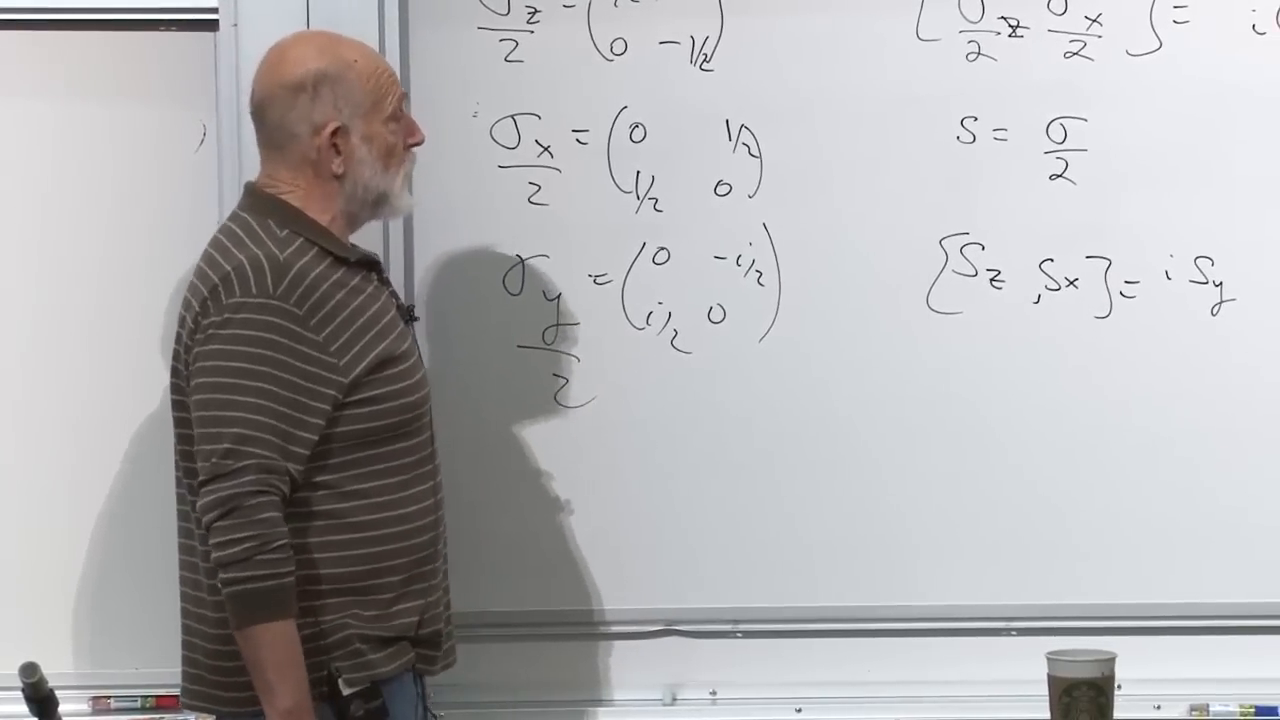
\includegraphics[width=0.9\linewidth]{lecture_04_frame_02.png}
\caption{En unidades en las que \(\hbar=1\), la mitad de las matrices de Pauli son los operadores de momento angular de espín uno medio y satisfacen \([S_z,S_x]=iS_y\).}
\lectureframe{00:55:41}
\end{figure}

Las dos ecuaciones de autovalores de \(S_z\) son
\begin{equation}
S_z\lvert\pm\rangle
=\pm\frac{\hbar}{2}\lvert\pm\rangle.
\end{equation}
Equivalentemente, el número cuántico magnético adimensional es
\begin{equation}
m_{s}=\pm\frac12,
\qquad
S_{z}\lvert m_{s}\rangle
=m_{s}\hbar\,\lvert m_{s}\rangle.
\end{equation}
Los operadores de subida y bajada del momento angular desplazan \(m\) en pasos enteros, pero esto no exige que todas las escaleras pasen por cero. Los multipletes de espín entero contienen valores enteros de \(m\), mientras que los multipletes de espín semientero contienen valores semienteros. Para el espín uno medio, la escalera tiene solo los dos estados \(m_s=+1/2\) y \(m_s=-1/2\).

Estos dos estados forman el doblete de espín uno medio. Los electrones, muones, neutrinos y quarks se cuentan entre las partículas descritas por multipletes de espín semientero.

\section{Momento angular orbital y de espín}

Ahora hay dos tipos de momento angular. El momento angular orbital describe el movimiento respecto de un origen,
\begin{equation}
\mathbf L=\mathbf R\times\mathbf P,
\end{equation}
mientras que \(\mathbf S\) es espín intrínseco. Su suma vectorial es el momento angular total,
\begin{equation}
\mathbf J=\mathbf L+\mathbf S.
\end{equation}

\begin{classroomqa}
\lecturetimestamp{00:56:49}
\audiencequestion{Si un sistema tiene momento angular total \(\mathbf J\), ¿cómo se identifica su espín \(\mathbf S\)?}
\lecturerresponse{Por lo general, los números cuánticos de espín y orbital se especifican por separado. Si \(L=0\), todo el momento angular es espín. De lo contrario, se necesitan las reglas cuánticas para sumar momentos angulares, que se dejan para más adelante.}
\end{classroomqa}

Las reglas de suma se aplican por igual al momento angular orbital más el espín, a dos espines o a dos momentos angulares orbitales. El sistema combinado tiene sus propios valores permitidos de momento angular total, pero aún no hacen falta esas reglas.

\begin{classroomqa}
\lecturetimestamp{00:58:18}
\audiencequestion{¿Qué evidencia experimental llevó a introducir el espín?}
\lecturerresponse{La espectroscopia aportó evidencia, pero la tabla periódica ofrece una motivación particularmente clara: su estructura de capas exige que los electrones tengan una propiedad adicional de dos valores.}
\end{classroomqa}

\section{Degeneración hidrogenoide y conteo de capas}

Para el momento angular orbital, la ecuación de autovalores de \(L^{2}\) es
\begin{equation}
L^{2}\lvert\ell,m\rangle
=\hbar^{2}\ell(\ell+1)\lvert\ell,m\rangle,
\end{equation}
y un valor fijo de \(\ell\) tiene
\begin{equation}
2\ell+1
\end{equation}
estados magnéticos, correspondientes a \(m=-\ell,-\ell+1,\ldots,\ell\).

El problema de Coulomb no relativista ideal presenta una degeneración adicional. Las energías de los estados ligados son negativas y se acercan a cero desde abajo, pero para el conteo solo importa cómo se alinean los niveles. El primer nivel \(\ell=1\) se alinea con el siguiente nivel \(\ell=0\); el primer nivel \(\ell=2\) se suma a la siguiente capa principal, y el patrón continúa.\footnote{\texttt{\_04\_\_03}, \(01{:}02{:}01\); la alineación completa de las capas principales se indica desde \(01{:}02{:}33\) hasta \(01{:}04{:}10\).}

\begin{figure}[htbp]
\centering
\begin{tikzpicture}[x=1.55cm,y=1.0cm]
\draw[->] (-0.65,0) -- (-0.65,4.35);
\draw[->] (-0.85,0) -- (4.75,0);
\node at (-0.95,4.08) {\(E\)};
\node at (4.55,-0.28) {\(\ell\)};
\node at (0,-0.30) {\(0\)};
\node at (2,-0.30) {\(1\)};
\node at (4,-0.30) {\(2\)};

\draw (-0.20,0.75) -- (0.20,0.75);

\draw (-0.20,2.00) -- (0.20,2.00);
\foreach \dx in {-0.18,0,0.18}
  \draw (2+\dx-0.06,2.00) -- (2+\dx+0.06,2.00);

\draw (-0.20,3.15) -- (0.20,3.15);
\foreach \dx in {-0.18,0,0.18}
  \draw (2+\dx-0.06,3.15) -- (2+\dx+0.06,3.15);
\foreach \dx in {-0.32,-0.16,0,0.16,0.32}
  \draw (4+\dx-0.05,3.15) -- (4+\dx+0.05,3.15);

\node[anchor=west] at (0.35,0.75) {\(n=1\)};
\node[anchor=west] at (2.35,2.00) {\(n=2\)};
\node[anchor=west] at (4.40,3.15) {\(n=3\)};
\end{tikzpicture}
\caption{Las tres primeras capas de Coulomb ideales combinan multipletes orbitales con la misma energía principal: un estado en la primera capa, \(1+3\) en la segunda y \(1+3+5\) en la tercera.}
\lectureframe{01:02:01}
\end{figure}

En la capa principal \(n\), los valores orbitales permitidos son\footnote{Este intervalo compacto de \(\ell\) y la suma que aparece a continuación reconstruyen las alineaciones de niveles y los conteos \(1,4,9,16,\ldots\) indicados desde \(01{:}02{:}33\) hasta \(01{:}04{:}10\). El comienzo del diagrama del espectro aparece en \texttt{\_04\_\_03} en \(01{:}02{:}01\).}
\[
\ell=0,1,\ldots,n-1.
\]
Por tanto, el número de estados espaciales es
\begin{equation}
\sum_{\ell=0}^{n-1}(2\ell+1)=n^{2},
\end{equation}
lo que da la secuencia
\begin{equation}
1,\ 4,\ 9,\ 16,\ldots .
\end{equation}
Este conteo solo incluye los estados orbitales. Cada estado espacial admite dos valores de espín, así que los totales idealizados correspondientes son
\begin{equation}
2,\ 8,\ 18,\ 32,\ldots=2n^{2}.
\end{equation}

\section{Exclusión y la propiedad electrónica de dos valores}

Empecemos con el helio en la aproximación de electrones independientes. Su núcleo tiene el doble de carga protónica, lo que reescala los niveles hidrogenoides y atrae los electrones hacia el interior. Si por el momento ignoramos las interacciones electrón--electrón, dos electrones pueden ocupar el orbital espacial más bajo y dar una aproximación inicial razonable al estado fundamental del helio.

¿Por qué no colocar también allí un tercer electrón? Eso reduciría su energía orbital, pero no ocurre. La restricción es el principio de exclusión de Pauli: dos electrones no pueden ocupar el mismo estado completo de una partícula. Sería engañoso describir esto como una fuerza repulsiva ordinaria. Es una restricción sobre los estados cuánticos permitidos.

Parece haber una contradicción. Los dos electrones del helio sí comparten el mismo orbital espacial. La resolución está en que un estado electrónico completo contiene más que la función de onda orbital: también contiene un grado de libertad con dos valores. Llamémoslos espín arriba y espín abajo. Un electrón en el orbital más bajo puede tener espín arriba y el otro espín abajo; sus estados espaciales coinciden, pero sus estados cuánticos completos no.

En este punto, el conteo avanza hacia el litio y luego retrocede. Ese retroceso deja claro por qué hacen falta tanto la exclusión como el espín. Imaginemos una regla de exclusión sin espín. Solo un electrón podría ocupar el estado espacial más bajo. Un segundo tendría que entrar en uno de los cuatro estados espaciales de la siguiente capa principal, lo que daría varias alternativas en lugar del estado fundamental único que se observa en el helio. Esa versión de la exclusión sin espín es incorrecta.

Restituyamos los dos valores de espín. Dos electrones llenan el orbital más bajo con espines opuestos. Un tercer electrón, como en el litio neutro, debe entrar en la siguiente capa principal. Esa capa tiene un estado espacial \(\ell=0\) y tres estados espaciales \(\ell=1\). Antes de contar el espín, hay cuatro posibilidades.

\begin{classroomqa}
\lecturetimestamp{01:14:58}
\audiencequestion{¿Cómo dan los estados \(s\) y \(p\) ocho posibilidades en la primera capa excitada?}
\lecturerresponse{Hay un estado espacial con \(\ell=0\) y tres con \(\ell=1\), lo que da cuatro estados espaciales. Cada uno admite dos valores de espín, así que el total es \(2(1+3)=8\).}
\end{classroomqa}

Este es el sencillo conteo que explica las ocho casillas de la segunda fila de la tabla periódica. Se trata deliberadamente de una idealización: el análisis posterior dejará claro que las interacciones electrón--electrón pronto invalidan la imagen de capas hidrogenoides independientes.

La propiedad de dos valores también se puede comprobar como momento angular. El espín del electrón va acompañado de un momento magnético, así que un campo magnético asigna energías distintas a sus dos proyecciones de espín. Un nivel degenerado en ausencia de campo se desdobla en dos, tal como se espera para un momento magnético pequeño alineado o antialineado con el campo. Este desdoblamiento permite comprobar si el grado de libertad añadido de dos valores se comporta como un momento angular y no como una etiqueta binaria arbitraria.

\section{Fotones, electrones y los límites del modelo de capas}

No todas las partículas obedecen la misma regla de ocupación. Muchos fotones pueden ocupar el mismo modo electromagnético; una onda luminosa clásica puede entenderse como un estado que contiene un gran número de fotones en ese modo. Los electrones se comportan de otra manera: la exclusión les impide acumularse en un mismo estado cuántico completo. Este contraste motiva la distinción entre las dos estadísticas de partículas.

\begin{classroomqa}
\lecturetimestamp{01:20:28}
\audiencequestion{¿Qué ocurre con un flujo de electrones libres, en vez de electrones ligados a átomos?}
\lecturerresponse{La regla de exclusión sigue vigente: los electrones no pueden ocupar todos un mismo estado cuántico. Un láser puede poner muchos fotones en el mismo modo, pero no se puede preparar así un flujo de electrones.}
\end{classroomqa}

La restricción es una propiedad de los electrones, no una particularidad de la ligadura atómica.

\begin{classroomqa}
\lecturetimestamp{01:21:12}
\audiencequestion{¿El momento angular orbital describe específicamente la rotación alrededor de un núcleo?}
\lecturerresponse{El momento angular se define respecto de un origen elegido. En un átomo, el núcleo es el origen natural; una partícula libre tiene momento angular \(\mathbf R\times\mathbf P\) respecto del origen que se elija.}
\end{classroomqa}

Toda descripción de una rotación elige un punto respecto del cual se realiza. Un átomo proporciona un centro natural porque su núcleo es el centro del potencial aproximadamente central. En el espacio libre no hay ningún origen privilegiado, aunque se puede calcular el momento angular respecto de cualquiera que se elija.

\begin{classroomqa}
\lecturetimestamp{01:22:34}
\audiencequestion{¿Por qué la tabla periódica tiene filas repetidas de ocho elementos y luego filas repetidas de dieciocho?}
\lecturerresponse{El modelo sencillo de capas de electrones independientes no explica el patrón completo. Falla pronto porque desprecia las interacciones entre los electrones.}
\end{classroomqa}

En un átomo grande, los electrones exteriores interactúan tanto con una nube electrónica interior considerable como con el núcleo. Ya no tiene sentido tratar cada electrón como si se moviera independientemente en un campo de Coulomb sin apantallamiento.

\begin{classroomqa}
\lecturetimestamp{01:23:33}
\audiencequestion{¿Por qué los átomos no se vuelven muchísimo más grandes al añadir más electrones?}
\lecturerresponse{Al añadir electrones también se añaden protones al núcleo. El aumento de la carga nuclear atrae hacia el interior los electrones internos, que a su vez apantallan el núcleo. En esta imagen sencilla, un electrón de valencia exterior se mueve entonces en una carga efectiva de aproximadamente una unidad.}
\end{classroomqa}

El aumento de la carga nuclear contrae la nube interna. En un átomo con un electrón de valencia exterior, el núcleo y los electrones internos casi se cancelan a grandes distancias, de modo que el electrón de valencia queda en un campo parecido al de una carga positiva de una unidad. Por tanto, el tamaño atómico no crece simplemente en proporción al número de electrones.

\begin{classroomqa}
\lecturetimestamp{01:24:49}
\audiencequestion{¿Es la repulsión eléctrica la razón por la que los átomos vecinos permanecen separados?}
\lecturerresponse{No por sí sola. La exclusión de Pauli produce una repulsión efectiva importante cuando se solapan las nubes electrónicas y, para muchos átomos, es la razón dominante por la que estas se resisten a solaparse más.}
\end{classroomqa}

La repulsión de Pauli es una consecuencia efectiva de la exclusión, no una ley de fuerza adicional.

\begin{classroomqa}
\lecturetimestamp{01:25:23}
\audiencequestion{¿Es el principio de exclusión un postulado independiente?}
\lecturerresponse{En la mecánica cuántica no relativista se impone como postulado. En la teoría cuántica relativista, la conexión espín--estadística le proporciona un fundamento más profundo.}
\end{classroomqa}

\section{Partículas idénticas en la mecánica clásica y cuántica}

Antes de formular ese postulado, veamos cómo se cuentan clásicamente las partículas idénticas. Coloquemos dos partículas del mismo tipo en un conjunto de cajas. Si las partículas llevaran nombres ocultos---Harry y Sally---, parecería que Harry en la primera caja y Sally en la segunda es distinto de Sally en la primera y Harry en la segunda.

La mecánica clásica permite esa imagen, aunque las etiquetas sean demasiado tenues para detectarlas. Se puede imaginar una marca arbitrariamente débil en cada partícula y aun así considerar distintas sus trayectorias. En mecánica estadística clásica, por lo general se elige no contar las permutaciones de partículas idénticas como configuraciones nuevas. Para \(N\) partículas, esta convención produce el conocido factor \(1/N!\).

La mecánica cuántica es más estricta. Las partículas idénticas no llevan etiquetas individuales ocultas que, en principio, puedan seguirse. Dos electrones son intercambiables en cuanto electrones. Intercambiar un electrón por un fotón produciría una configuración físicamente distinta porque pertenecen a especies distintas; en cambio, intercambiar las dos posiciones electrónicas no permite saber cuál de los electrones estaba en cada una.

Un estado de una partícula tiene una función de onda
\[
\psi(x)=\langle x\vert\psi\rangle.
\]
Para dos partículas, el estado es una función de dos argumentos de posición,
\begin{equation}
\psi(x_{1},x_{2}).
\end{equation}
Los subíndices etiquetan las dos posiciones en la descripción, no dos direcciones espaciales. Su módulo al cuadrado da la densidad de probabilidad conjunta de posición.

\section{El operador de intercambio y el postulado de estadística}

Intercambiemos las posiciones de las dos partículas:
\begin{equation}
\psi(x_{1},x_{2})\longmapsto\psi(x_{2},x_{1}).
\end{equation}
Siguiendo la notación usada en este análisis, llamemos \(S\) al operador de intercambio. Aquí \(S\) denota el intercambio, no el vector de espín \(\mathbf S\). Su acción es
\begin{equation}
(S\psi)(x_{1},x_{2})=\psi(x_{2},x_{1}).
\end{equation}
Una función general de dos variables no tiene por qué ser simétrica, así que esta operación puede producir una función de onda distinta.

Al intercambiar dos veces se restablece el orden original:
\begin{equation}
S^{2}=I.
\end{equation}
El intercambio es reversible y conserva los productos internos, por lo que se representa mediante un operador unitario. Si \(\psi\) es un vector propio de \(S\) con autovalor \(\lambda\), entonces
\[
S^{2}\psi=\lambda^{2}\psi=\psi,
\]
y, por tanto,
\begin{equation}
\lambda=\pm1.
\end{equation}

Esta conclusión identifica dos subespacios propios del intercambio, pero no afirma que toda función de onda arbitraria de dos partículas sea ya un vector propio de \(S\). Cualquier función de onda de ese tipo puede descomponerse en sus dos partes,\footnote{Esta descomposición es una aclaración algebraica editorial de los dos subespacios propios que se desprenden de \(S^{2}=I\). La argumentación registrada enuncia los dos valores propios y, a continuación, introduce el principio adicional de la estadística.}
\begin{equation}
\psi_{\pm}=\frac12(I\pm S)\psi,
\end{equation}
que satisfacen
\begin{equation}
S\psi_{\pm}=\pm\psi_{\pm}.
\end{equation}
Por tanto,
\begin{align}
\psi_{+}(x_{2},x_{1})&=\psi_{+}(x_{1},x_{2}),\\
\psi_{-}(x_{2},x_{1})&=-\psi_{-}(x_{1},x_{2}).
\end{align}

Ahora se introduce un principio adicional, que no se desprende únicamente de \(S^{2}=I\). Para partículas idénticas de una misma especie, los estados permitidos pertenecen por completo a uno de estos sectores de intercambio: al intercambiar un par, la función de onda siempre vuelve a ser la misma o siempre cambia de signo. El sector \(+1\) es simétrico y el sector \(-1\) es antisimétrico. La interpretación física de estas dos posibilidades como las dos estadísticas de partículas es el paso siguiente y queda para la discusión posterior.

\chapter{Simetría de intercambio, espín y los dos signos menos}

\section{Llenado de capas y la cuestión de las estadísticas del espín--}

La revisión del modelo de capas comienza con dos propiedades asociadas a los electrones. El electrón tiene espín un medio, con las dos proyecciones de espín adimensionales
\begin{equation}
m_s=+\frac12,
\qquad
m_s=-\frac12,
\end{equation}
y los electrones obedecen el principio de exclusión de Pauli. Estos hechos están relacionados, pero no son la misma afirmación.

La expresión ``el mismo estado'' requiere precisión. Ningún par de electrones puede ocupar el mismo estado completo de una partícula. Sin embargo, dos electrones pueden compartir un orbital espacial si sus estados de espín son distintos. En la aproximación de electrones independientes para el helio, ambos electrones ocupan el orbital espacial más bajo, uno con espín hacia arriba y el otro con espín hacia abajo. Más precisamente, las alternativas ``el primero tiene espín hacia arriba y el segundo, hacia abajo'' y ``el primero tiene espín hacia abajo y el segundo, hacia arriba'' pertenecen a un estado de espín entrelazado de dos electrones.

Esta es solo la antigua aproximación del modelo de capas. Ignora la interacción entre los electrones y se usa aquí por su sencillez para contar. En el litio, los dos primeros electrones llenan el orbital espacial más bajo con espines opuestos. El tercero no puede ocupar ninguno de esos estados completos y debe ocupar un orbital de mayor energía.

El siguiente paso es el conocido diagrama del momento angular orbital. Los sectores con
\begin{equation}
\ell=0,\qquad \ell=1,\qquad \ell=2
\end{equation}
se llaman estados \(S\), \(P\) y \(D\). Para un valor fijo de \(\ell\) hay
\begin{equation}
2\ell+1
\end{equation}
estados orbitales, de modo que
\begin{equation}
\ell=0\Rightarrow 1,
\qquad
\ell=1\Rightarrow 3,
\qquad
\ell=2\Rightarrow 5.
\end{equation}
El problema de Coulomb tiene degeneraciones adicionales: niveles radiales de distintos sectores de \(\ell\) pueden tener la misma energía. Para el argumento sobre el llenado de capas, la siguiente capa contiene un orbital \(S\) y tres orbitales \(P\). Por tanto, tiene
\begin{equation}
1+3=4
\end{equation}
estados espaciales. El espín duplica el número:
\begin{equation}
2(1+3)=8.
\end{equation}

Esos ocho estados completos de una partícula se llenan en la progresión sencilla desde el litio hasta el neón. Más allá de la capa cerrada, el sodio vuelve a tener un electrón exterior, por lo que esta imagen rudimentaria hace que se parezca al litio. La química no es el objetivo. Lo importante es que el espín semientero y la exclusión aparecen juntos.

Los fotones ofrecen el contraste. Tienen espín entero y no obedecen una regla de exclusión. Una onda electromagnética clásica corresponde a muchos fotones que ocupan el mismo modo. Los bosones pueden acumularse en un estado común, mientras que los fermiones idénticos no pueden ocupar más de una vez un mismo estado completo. La pregunta es si esas dos asociaciones podrían haber sido distintas: espín semientero sin exclusión o espín entero con exclusión. En tres dimensiones espaciales, la relación entre espín-- y estadística dice que no. La afirmación conocida requiere matices en una y dos dimensiones espaciales, y aquí no se intenta demostrar el resultado de la teoría de campos.

\begin{classroomqa}
\lecturetimestamp{00:11:48}
\audiencequestion{¿Existe un número máximo de cuantos bosónicos que puedan ocupar un estado?}
\lecturerresponse{No. Los bosones no tienen límite de ocupación y tienden a acumularse en el mismo estado.}
\end{classroomqa}

\section{Funciones de onda de muchas partículas}

Abordaremos la conexión mediante dos signos menos: uno proviene del intercambio y el otro de la rotación. Empecemos por el intercambio y, por el momento, dejemos de lado el espín.

Sea \(x_i\) la posición de la partícula \(i\). El subíndice identifica a la partícula; no es una componente cartesiana. Las tres coordenadas espaciales se condensan en el símbolo \(x_i\). Una base de posiciones para \(n\) partículas es
\begin{equation}
\lvert x_1,x_2,\ldots,x_n\rangle.
\end{equation}
Para un estado abstracto \(\lvert\Psi\rangle\), la función de onda en coordenadas es
\begin{equation}
\psi(x_1,x_2,\ldots,x_n)
=
\langle x_1,x_2,\ldots,x_n\mid\Psi\rangle.
\end{equation}
Su módulo al cuadrado,
\begin{equation}
\bigl\lvert\psi(x_1,x_2,\ldots,x_n)\bigr\rvert^2,
\end{equation}
es la densidad de probabilidad conjunta de encontrar la partícula \(1\) en \(x_1\), la partícula \(2\) en \(x_2\), y así sucesivamente.

Supongamos ahora que las partículas son idénticas. Imaginemos primero que pintamos de azul un electrón y de rojo otro. Entonces ``\(x_1\)azul en \(x_2\)''`` podría distinguirse de \(x_2\)azul en \(x_1\)''. Los electrones reales no llevan esos colores ni etiquetas individuales. Intercambiar las etiquetas que usamos para llevar la cuenta no puede crear una nueva configuración física.

Una fase global no cambia las probabilidades ni los valores esperados. Por tanto, para un estado perteneciente a un sector de intercambio definido, la función de onda en coordenadas puede satisfacer
\begin{equation}
\psi(x_2,x_1)=\eta\,\psi(x_1,x_2),
\qquad
\lvert\eta\rvert=1.
\end{equation}
Aplicar dos veces el mismo intercambio devuelve los argumentos originales y da
\begin{equation}
\eta^2=1,
\end{equation}
Así, los dos valores propios posibles para el intercambio son
\begin{equation}
\eta=+1
\qquad\hbox{or}\qquad
\eta=-1.
\end{equation}

\editorialnote{El álgebra del doble intercambio determina los valores propios posibles solo después de suponer que el estado tiene un comportamiento de intercambio definido. La restricción adicional de que los estados permitidos de una especie dada pertenezcan a un único sector de intercambio es una regla física; no se deduce de \(\eta^2=1\) por sí sola. La misma precisión se aplica al argumento de exclusión que sigue: la antisimetría implica exclusión una vez seleccionado el sector fermiónico, pero el álgebra del intercambio por sí sola no selecciona ese sector.}

Para los bosones, las funciones de onda permitidas son simétricas,
\begin{equation}
\psi_B(x_1,x_2)=\psi_B(x_2,x_1),
\end{equation}
mientras que para los fermiones son antisimétricas,
\begin{equation}
\psi_F(x_1,x_2)=-\psi_F(x_2,x_1).
\end{equation}
El signo menos no se aprecia cuando multiplica el estado entero, pero sí importa al sumar amplitudes. Así es como la simetría de intercambio adquiere consecuencias observables.

\section{Productos, sumas y exclusión}

Consideremos primero dos partículas asignadas al mismo orbital de una partícula \(\psi_0\). Su producto es
\begin{equation}
\psi_0(x_1)\psi_0(x_2).
\end{equation}
Al intercambiar las coordenadas de las partículas se obtiene
\begin{equation}
\psi_0(x_2)\psi_0(x_1)
=
\psi_0(x_1)\psi_0(x_2).
\end{equation}
Los valores de la función de onda son números, no operadores, así que los factores conmutan. El producto para el mismo estado es simétrico. Es una forma permitida para los bosones, pero no puede describir dos fermiones idénticos.

Asignemos ahora las partículas a orbitales distintos de una partícula:
\begin{equation}
\psi_0(x_1)\psi_1(x_2).
\end{equation}
El intercambio produce
\begin{equation}
\psi_0(x_2)\psi_1(x_1).
\end{equation}
Si las funciones son distintas, el producto intercambiado, en general, no es ni la expresión original ni su opuesta. Por tanto, el producto sin más no tiene ninguna de las simetrías de intercambio requeridas. Esto no impide que una partícula ocupe \(\psi_0\) mientras otra ocupa \(\psi_1\). Significa que el estado de dos partículas debe combinar las dos asignaciones.

La combinación simétrica es
\begin{equation}
\psi_B^{(01)}(x_1,x_2)
\propto
\psi_0(x_1)\psi_1(x_2)
+
\psi_0(x_2)\psi_1(x_1),
\end{equation}
y la combinación antisimétrica es
\begin{equation}
\psi_F^{(01)}(x_1,x_2)
\propto
\psi_0(x_1)\psi_1(x_2)
-
\psi_0(x_2)\psi_1(x_1).
\end{equation}
Los signos de proporcionalidad bastan, porque para el argumento sobre el intercambio no hace falta normalizar. Ambos estados contienen una partícula en cada orbital; solo difieren en cómo combinan las dos asignaciones indistinguibles.

Hagamos coincidir ahora los orbitales. La combinación bosónica se convierte en
\begin{align}
\psi_B^{(00)}(x_1,x_2)
&\propto
\psi_0(x_1)\psi_0(x_2)
+
\psi_0(x_2)\psi_0(x_1)\\
&=
2\psi_0(x_1)\psi_0(x_2),
\end{align}
que no es nula. La combinación fermiónica da
\begin{align}
\psi_F^{(00)}(x_1,x_2)
&\propto
\psi_0(x_1)\psi_0(x_2)
-
\psi_0(x_2)\psi_0(x_1)\\
&=0.
\end{align}
Con la regla de intercambio antisimétrica, se deduce la exclusión: no existe un estado antisimétrico no nulo en el que ambos fermiones estén en el mismo estado de una partícula.

Para un estado de muchas partículas, la regla se aplica a cualquier transposición de dos argumentos. Una transposición deja inalterada una función de onda bosónica y cambia el signo de una fermiónica. Repetir la misma transposición no produce ningún cambio en ninguno de los dos casos. Lo sorprendente es que un solo intercambio, aunque no cambie ninguna etiqueta observable de las partículas, cambia el signo de un estado fermiónico.

\section{El espín en la etiqueta completa de la partícula}

Ahora podemos reincorporar el espín con un pequeño cambio. La amplitud de una partícula depende tanto de la posición como de una etiqueta discreta de espín,
\begin{equation}
\psi(x,\sigma),
\end{equation}
donde \(\sigma=+1\) o \(-1\) indica el resultado elegido para \(\sigma_z\). El módulo al cuadrado es la densidad de probabilidad conjunta para la posición y la etiqueta de espín especificadas.

Para muchas partículas, la función de onda es
\begin{equation}
\psi(x_1,\sigma_1;\,x_2,\sigma_2;\,\ldots).
\end{equation}
El intercambio permuta todo lo que pertenece a las dos partículas, no solo sus posiciones:
\begin{align}
\psi_B(x_1,\sigma_1;\,x_2,\sigma_2)
&=
+\psi_B(x_2,\sigma_2;\,x_1,\sigma_1),\\
\psi_F(x_1,\sigma_1;\,x_2,\sigma_2)
&=
-\psi_F(x_2,\sigma_2;\,x_1,\sigma_1).
\end{align}
Esta es la formulación precisa de la afirmación inicial sobre el modelo de capas. Dos electrones pueden compartir un orbital espacial solo si sus estados completos, incluido el espín, son distintos.

\begin{classroomqa}
\lecturetimestamp{00:34:33}
\audiencequestion{¿Es la simetría de intercambio un caso particular del grupo de permutaciones?}
\lecturerresponse{Sí. Intercambiar partículas es una permutación, y la ley de transformación con signo más o menos da una representación del grupo de permutaciones.}
\end{classroomqa}

\begin{classroomqa}
\lecturetimestamp{00:35:12}
\audiencequestion{¿Por qué la construcción de dos partículas es un producto y no una suma de las funciones de onda de una partícula?}
\lecturerresponse{Una suma describe una partícula en una superposición. Un producto pertenece al espacio producto tensorial de dos partículas y describe una partícula asignada a cada estado de una partícula.}
\end{classroomqa}

El intercambio de las etiquetas completas se muestra en la pizarra de abajo.\footnote{El orden de las etiquetas de posición--espín se reconstruye a partir del fotograma legible de la pizarra y de la explicación circundante, desde 00:33:43 hasta 00:34:25.}
\begin{figure}[htbp]
\centering
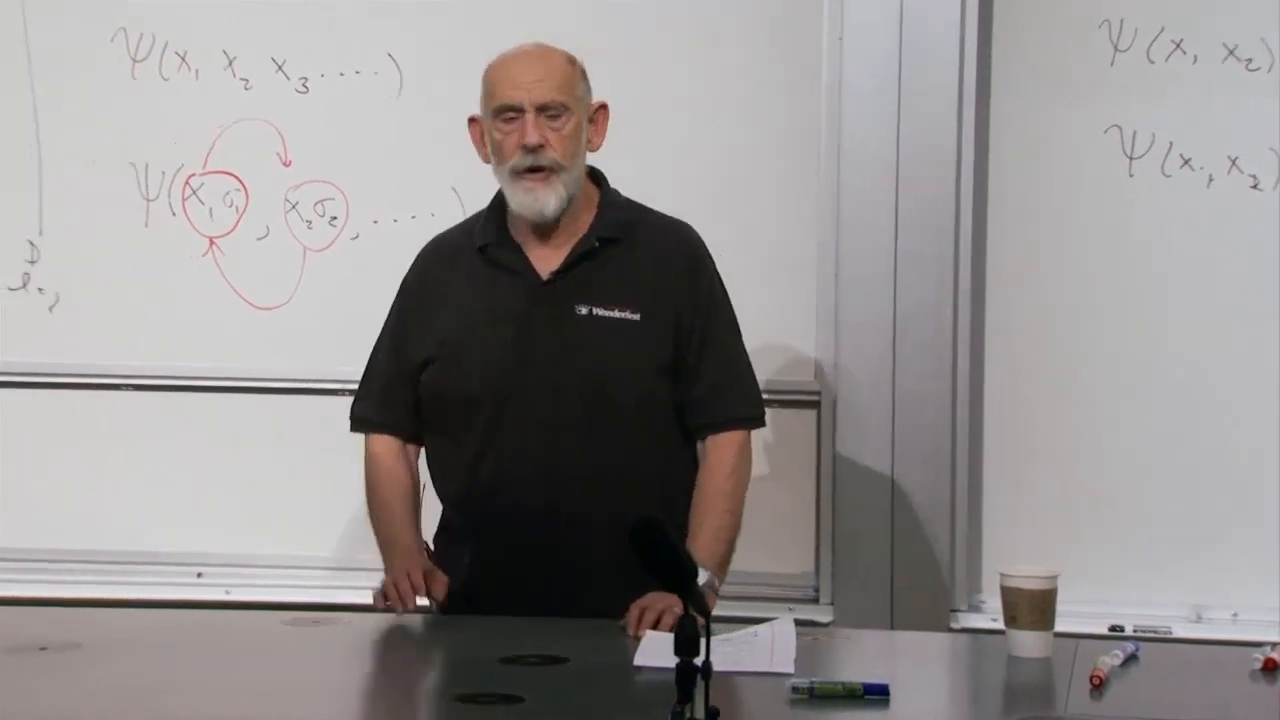
\includegraphics[width=0.9\linewidth]{lecture_05_frame_03.png}
\caption{Al intercambiar dos partículas idénticas se permutan sus etiquetas completas de posición--espín. Un estado bosónico permanece inalterado, mientras que uno fermiónico cambia de signo.}
\lectureframe{00:35:25}
\end{figure}

Estos son dos usos distintos de la linealidad. Para una partícula,
\begin{equation}
\alpha\psi_0(x)+\beta\psi_1(x)
\end{equation}
es una superposición de dos alternativas. Para dos partículas,
\begin{equation}
\psi_0(x_1)\psi_1(x_2)
\end{equation}
es una amplitud producto en un espacio con dos coordenadas de partícula. La simetrización o antisimetrización combina ese producto con su versión intercambiada.

\begin{classroomqa}
\lecturetimestamp{00:36:13}
\audiencequestion{¿El intercambio de partículas produce un efecto de interferencia?}
\lecturerresponse{Sí. La amplitud fermiónica nula para el mismo estado puede entenderse como interferencia destructiva entre las dos contribuciones intercambiadas.}
\end{classroomqa}

\begin{classroomqa}
\lecturetimestamp{00:37:13}
\audiencequestion{¿Derivó Pauli la exclusión mediante este mismo argumento de simetría?}
\lecturerresponse{Pauli partió de un hecho empírico y encontró un marco matemático en el que podía expresarse. Al principio no estaba derivando la exclusión de una teoría más fundamental.}
\end{classroomqa}

La antisimetría proporciona el marco matemático en el que se expresa la regla empírica de exclusión.

\begin{classroomqa}
\lecturetimestamp{00:39:01}
\audiencequestion{¿Está relacionada la interferencia por intercambio de partículas con la interferencia entre caminos alternativos?}
\lecturerresponse{Sí. En una historia, las dos partículas pasan sin cruzarse; en otra, se cruzan y llegan a los destinos intercambiados. Las amplitudes se suman para los bosones y pueden cancelarse para los fermiones.}
\end{classroomqa}

El intercambio aporta el primer signo menos. La rotación aporta el segundo.

\section{El segundo signo menos: rotación de \texorpdfstring{\(2\pi\)}{2 pi}}

Una rotación completa parece no producir ningún efecto. Toda dirección geométrica ordinaria vuelve a su posición inicial tras un ángulo de \(2\pi\). Sin embargo, lo que debe volver a sus valores iniciales son las probabilidades y los valores esperados. El propio vector de estado puede volver con una fase global, igual que puede hacerlo tras un intercambio.

\begin{classroomqa}
\lecturetimestamp{00:42:12}
\audiencequestion{¿Qué eje se usa para la rotación y cuál es el generador: el momento angular orbital, el espín o ambos?}
\lecturerresponse{Se puede elegir un eje externo; aquí tomaremos el eje \(z\). El generador es el momento angular total, que incluye las contribuciones orbital y de espín. El espín no tiene por qué apuntar a lo largo del eje elegido.}
\end{classroomqa}

\editorialnote{En esta discusión, las fórmulas del momento angular usan \(\hbar=1\), de modo que \(m\) es el valor propio adimensional de \(J_z\).}

Sea \(\psi(\theta)\) el estado obtenido al variar el parámetro de rotación a lo largo de un ángulo \(\theta\). Con la convención usada aquí,
\begin{equation}
J_z\psi(\theta)
=
-i\frac{\partial}{\partial\theta}\psi(\theta).
\end{equation}
Para un estado con \(J_z\) definido,
\begin{equation}
J_z\psi(\theta)=m\psi(\theta).
\end{equation}
Al combinar las ecuaciones se obtiene
\begin{equation}
-i\frac{\partial}{\partial\theta}\psi(\theta)
=
m\psi(\theta),
\end{equation}
cuya solución es
\begin{equation}
\psi(\theta)=e^{im\theta}\psi(0).
\end{equation}

Los valores permitidos de \(m\) son enteros o semienteros. Por tanto,
\begin{equation}
\psi(2\pi)
=
\begin{cases}
+\psi(0), & m\in\mathbb Z,\\[4pt]
-\psi(0), & m\in\mathbb Z+\tfrac12.
\end{cases}
\end{equation}
Tras otra vuelta completa,
\begin{equation}
\psi(4\pi)=\psi(0)
\end{equation}
en cualquiera de los dos casos. Este es el segundo signo menos: un estado de un multiplete de momento angular semientero cambia de signo bajo una rotación de \(2\pi\).

El signo no altera \(\lvert\psi\rvert^2\), así que no se aprecia cuando multiplica el estado entero. Aun así, una rotación de \(2\pi\) no está representada por la identidad en un estado de espín semientero. La diferencia se vuelve observable cuando el signo es relativo a otra amplitud coherente.

\section{Los caminos de \texorpdfstring{\(2\pi\) y \(4\pi\)}{2 pi y 4 pi}}

La diferencia entre \(2\pi\) y \(4\pi\) puede hacerse visible sin más álgebra. Sostén una taza con una mano y gírala una vuelta completa sin soltarla. La taza recupera su orientación original, pero el brazo queda retorcido. Continúa con una segunda vuelta y podrás devolver el brazo a su posición original sin invertir el movimiento de la taza.

Una construcción relacionada consiste en colocar una esfera dentro de una caja y unirla a la caja con cuerdas. Al girar la esfera \(2\pi\), las cuerdas quedan enredadas. En el espacio tridimensional ordinario, puede deshacerse el enredo asociado a un giro de \(4\pi\). El objeto pertinente no es simplemente la orientación final de la esfera, sino el camino recorrido por el espacio de rotaciones.

\begin{classroomqa}
\lecturetimestamp{00:54:22}
\audiencequestion{Si se gira la esfera dos veces alrededor del mismo eje, ¿se pueden desenredar realmente las cuerdas? ¿Hace falta otra dimensión espacial?}
\lecturerresponse{El camino de \(4\pi\) puede deshacerse en el espacio tridimensional ordinario. El tiempo parametriza el movimiento; no es otra dirección espacial. Un camino de \(2\pi\) no puede deshacerse de este modo, mientras que uno de \(4\pi\) sí puede.}
\end{classroomqa}

Las demostraciones distinguen un camino no trivial de \(2\pi\) de un camino deshacible de \(4\pi\), sin desarrollar una teoría formal del grupo de rotaciones.

\section{Intercambio y rotación en la imagen de la correa}

Ahora aparecen juntos los dos signos menos. Intercambiar dos fermiones idénticos cambia el signo de su función de onda conjunta. Girar un estado de espín semientero en \(2\pi\) también cambia su signo. Una correa establece una relación geométrica entre ambas operaciones.

Dispón la correa de modo que se hayan intercambiado sus dos extremos inferiores. Vista de otro modo, la misma correa tiene un giro de \(2\pi\). Al efectuar el intercambio junto con la rotación de \(2\pi\), se elimina el giro y la correa queda sin torsión. El proceso combinado puede reducirse continuamente a no hacer nada.\footnote{La observación sobre el intercambio--la rotación se atribuye a David Finkelstein en la conferencia. El registro de la fuente no identifica ninguna publicación concreta, por lo que aquí el nombre se conserva únicamente como parte de esa atribución.}

\begin{classroomqa}
\lecturetimestamp{01:01:12}
\audiencequestion{¿Se trata solo de cómo está incrustada la correa en el espacio, y no de una afirmación sobre la topología de las partículas?}
\lecturerresponse{La correa puede interpretarse como una historia de partículas en el espacio-tiempo. Si el tiempo avanza hacia arriba, una sección transversal muestra objetos parecidos a partículas. Se crean pares, se gira un objeto en \(2\pi\) y se intercambian dos objetos idénticos. En esa historia, las fases de rotación e intercambio se cancelan.}
\end{classroomqa}

La historia hace explícito el cómputo de las fases. Empecemos sin partículas. En dos lugares separados, creemos un par partícula--antipartícula, de modo que en un instante intermedio haya cuatro partículas. Giremos una partícula en \(2\pi\) mientras intercambiamos dos partículas idénticas en otro lugar de la configuración. La historia completa puede deformarse hasta la historia elemental en que se crea un par y luego se aniquila. En el cómputo de signos aquí considerado, esa historia trivial no tiene fase adicional. Si \(\eta_{\mathrm{rot}}\) y \(\eta_{\mathrm{ex}}\) representan los dos signos, la cancelación expuesta oralmente puede escribirse de forma compacta como sigue:\footnote{Esta ecuación de fase expresa la cancelación descrita desde 01:06:50 hasta 01:07:18; la conferencia presenta la construcción como sugerente, no como una demostración rigurosa.}
\begin{equation}
\eta_{\mathrm{rot}}\eta_{\mathrm{ex}}=1.
\end{equation}

\begin{classroomqa}
\lecturetimestamp{01:03:34}
\audiencequestion{¿Puede relacionarse el intercambio con las rotaciones haciendo que cada una de dos partículas gire \(\pi\) y luego reorientándolas?}
\lecturerresponse{Esa construcción quizá refleje matemáticas relacionadas, pero utiliza dos rotaciones separadas de \(\pi\). El proceso que analizamos aquí contiene una rotación de \(2\pi\), así que los dos argumentos no son idénticos.}
\end{classroomqa}

El argumento depende de que sea posible crear y aniquilar objetos parecidos a partículas. No tendría esta forma en una teoría en la que las partículas fueran eternas. Tampoco se presenta como la demostración habitual del teorema de espín--estadística. Su propósito es mostrar una razón topológica por la que los signos de intercambio y rotación concuerdan.

\section{Bultos, imágenes especulares y aniquilación}

La construcción puede repetirse con configuraciones localizadas de campos. Supongamos que uno o más campos adoptan sus valores de vacío casi en todas partes, pero presentan forma y estructura no nulas en una región pequeña. Esa configuración localizada es un bulto.

Construyamos ahora una segunda configuración que sea la imagen especular apropiada de la primera. Llamemos partícula a una y antipartícula a la otra. Acerquémoslas. Las partes correspondientes de las configuraciones de campo se encuentran y se deshacen mutuamente. En una etapa intermedia, algunas partes de los bultos pueden haber desaparecido mientras otras permanecen. Si continuamos la deformación, se elimina la estructura restante y los campos vuelven a la configuración de vacío. Dos torsiones opuestas en una correa dan la misma imagen: al empujarlas una hacia la otra, se deshacen.

El proceso puede recorrerse en sentido inverso. El espacio vacío puede producir un bulto y su compañero especular. Se pueden crear dos pares de este tipo, girar un bulto en \(2\pi\), intercambiar dos bultos idénticos y volver a aniquilar los pares. Se aplica entonces la misma cancelación entre intercambio--rotación. Esto sigue siendo una extensión heurística de la construcción, no un teorema sobre toda excitación localizada.

\begin{classroomqa}
\lecturetimestamp{01:11:30}
\audiencequestion{¿Existen realizaciones físicas de estas configuraciones de campo parecidas a bultos?}
\lecturerresponse{Sí. Algunos ejemplos son los núcleos en descripciones de tipo Skyrmion, los monopolos magnéticos y otras excitaciones de campos parecidas a partículas.}
\end{classroomqa}

La imagen de los bultos especulares permite entender la generalización. Lo pertinente no es que el objeto empezara como una partícula puntual elemental, sino que una excitación parecida a una partícula y su compañera puedan crearse, acercarse y aniquilarse de manera continua. Esa característica motiva una relación más amplia entre el comportamiento bajo rotación y bajo intercambio.

\begin{classroomqa}
\lecturetimestamp{01:16:12}
\audiencequestion{¿Significa espín un medio que el estado acumula solo la mitad de la fase de rotación habitual?}
\lecturerresponse{En esta convención, la fase es \(e^{im\theta}\). Para \(m\) semientero, una rotación de \(2\pi\) da \(-1\), mientras que una rotación de \(4\pi\) da \(+1\).}
\end{classroomqa}

\section{Un signo global y un experimento nulo}

¿Se puede observar el signo menos de una rotación de \(2\pi\)? Empecemos con un experimento en el que no se puede. Confinemos un electrón en un campo magnético, dejemos que su espín siga el campo mientras el aparato gira lentamente en \(2\pi\) y, a continuación, liberemos el electrón en un dispositivo de interferencia. Comparemos esto con el mismo procedimiento sin la rotación.

La rotación transforma el estado así:
\begin{equation}
\psi\longmapsto-\psi,
\end{equation}
pero el signo menos multiplica el estado entero. Todas las probabilidades permanecen iguales, por lo que el patrón de interferencia final no conserva ningún indicio de si tuvo lugar la rotación preliminar. Es un experimento nulo: una fase común no tiene con qué interferir.

\begin{classroomqa}
\lecturetimestamp{01:20:01}
\audiencequestion{¿Por qué debe hacerse lentamente la rotación del campo magnético?}
\lecturerresponse{El espín debe seguir acompañando al campo magnético giratorio. Si el campo se arrastra demasiado rápido, el espín no permanecerá alineado con él.}
\end{classroomqa}

\section{Un electrón en dos ramas coherentes}

El signo se vuelve observable cuando es relativo. Hagamos pasar un electrón por un divisor de haz. Una parte de su función de onda sigue un camino y otra parte sigue otro:
\begin{equation}
\psi(x)=\psi_1(x)+\psi_2(x).
\end{equation}
Es un electrón, no dos. Se encuentra en una superposición coherente de dos alternativas. Hay que tener clara la diferencia: los dos paquetes no son dos partículas independientes.

Guiemos los dos paquetes hacia regiones separadas que contienen campos magnéticos. Giremos el campo de una región en \(2\pi\), dejando el otro sin cambios. Para un estado de espín semientero,
\begin{equation}
\psi_1(x)+\psi_2(x)
\longmapsto
\psi_1(x)-\psi_2(x),
\end{equation}
donde la rama girada se ha etiquetado como \(2\). Ahora el signo es relativo. Cuando los dos paquetes vuelvan a superponerse, la suma se habrá convertido en resta. Un punto de interferencia constructiva puede convertirse en uno de interferencia destructiva, o incluso en un nodo.

\begin{classroomqa}
\lecturetimestamp{01:23:46}
\audiencequestion{¿Qué se está girando si hay un solo electrón pero dos ramas de la función de onda?}
\lecturerresponse{El electrón se encuentra en una superposición coherente de dos alternativas localizadas. Se gira una rama y la otra no. Si se abren las cajas para averiguar cuál de las alternativas ocurrió, esa medición destruye la interferencia.}
\end{classroomqa}

Abrir las cajas solo revelaría que hay un electrón, en una u otra caja. Sin esa medición, ambas amplitudes permanecen en el estado. Al repetir el experimento, el patrón de interferencia se forma detección a detección. En un nodo producido por el signo menos relativo no se detecta ningún electrón.

\section{Precesión magnética e interferencia de doble rendija}

Una disposición esquemática más práctica sustituye el experimento de las cajas, extremadamente lento. Dividamos una onda coherente de electrones en dos caminos. En uno de ellos, hagamos pasar el electrón por una región magnética con el espín inicialmente transversal al campo. Entonces el espín precesa. Al elegir la intensidad del campo y el tiempo de tránsito, se puede hacer que el espín de esa rama complete una vuelta de \(2\pi\), mientras que la otra rama no experimenta tal giro.\footnote{La conferencia afirma que se había realizado un experimento relacionado con la fase espinorial y describe su principio, pero el registro de la fuente no identifica ningún artículo ni aparato concreto. Por tanto, este relato se limita a la construcción presentada en la conferencia.}

\begin{classroomqa}
\lecturetimestamp{01:27:05}
\audiencequestion{¿Cómo se puede determinar el camino del electrón único?}
\lecturerresponse{No se puede determinar sin arruinar el experimento. Cualquier medición que registre qué camino siguió el electrón destruye la interferencia.}
\end{classroomqa}

\begin{classroomqa}
\lecturetimestamp{01:27:50}
\audiencequestion{¿Qué es exactamente una rama de la función de onda y cómo produce el divisor dos ramas?}
\lecturerresponse{Una rama es un paquete de ondas localizado a lo largo de un camino. El divisor transforma la onda incidente en dos paquetes separados espacialmente, y los campos eléctricos o magnéticos pueden guiarlos por caminos distintos.}
\end{classroomqa}

Salvo por la región magnética, este es el experimento de la doble rendija. Una onda electrónica incidente se separa en dos paquetes. Las ondas salientes se propagan hacia una región común de detección, donde sus amplitudes se superponen. Sin rotación relativa, las amplitudes centrales pueden sumarse. Una rotación de espín de \(2\pi\) en uno de los caminos invierte una amplitud y puede hacer que esas mismas contribuciones se cancelen.

\begin{classroomqa}
\lecturetimestamp{01:30:46}
\audiencequestion{¿Cómo puede haber interferencia si el electrón viaja por tubos o rendijas distintos?}
\lecturerresponse{La detección final no revela el camino. Las dos amplitudes de onda salientes se propagan y se superponen en el detector. Mirar para averiguar qué camino siguió destruiría la interferencia.}
\end{classroomqa}

\begin{classroomqa}
\lecturetimestamp{01:33:22}
\audiencequestion{¿Debe el diámetro del tubo o de la rendija ser comparable a la longitud de onda del electrón?}
\lecturerresponse{En una realización literal de doble rendija basada en la difracción, la abertura debe ser lo bastante pequeña para producir la dispersión necesaria. El aparato que se describe es esquemático, no un diseño práctico.}
\end{classroomqa}

\begin{classroomqa}
\lecturetimestamp{01:33:44}
\audiencequestion{¿Una rotación de la polarización de los fotones de \(2\pi\) dejaría inalterado el patrón de interferencia?}
\lecturerresponse{Sí. Los fotones tienen espín entero, por lo que una rotación completa de \(2\pi\) no introduce el signo menos fermiónico.}
\end{classroomqa}

\begin{classroomqa}
\lecturetimestamp{01:34:12}
\audiencequestion{¿En qué se aparta ligeramente el experimento práctico de la versión idealizada?}
\lecturerresponse{En el montaje ideal, el espín gira adiabáticamente. En la descripción práctica, el electrón atraviesa una región magnética y su espín precesa más rápidamente, pero la fase medida sigue siendo la asociada a un giro de \(2\pi\).}
\end{classroomqa}

El montaje lento aísla la idea al garantizar que el espín siga al campo sin movimiento adicional. El montaje con precesión produce dinámicamente el mismo signo relativo. En cualquiera de las dos versiones, las dos trayectorias deben dejar de ser distinguibles antes de que pueda aparecer un patrón de interferencia.

\begin{classroomqa}
\lecturetimestamp{01:36:15}
\audiencequestion{¿Es necesario recombinar las dos ramas después del divisor?}
\lecturerresponse{Sí. Los paquetes de ondas que emergen deben solaparse o extenderse sobre una región común de detección para que sus amplitudes puedan formar un patrón de interferencia.}
\end{classroomqa}

\begin{classroomqa}
\lecturetimestamp{01:38:12}
\audiencequestion{¿Es este experimento de rotación con un solo electrón una consecuencia del principio de exclusión de Pauli?}
\lecturerresponse{No. Solo hay un electrón. El experimento mide la fase del espinor bajo rotación, no la exclusión de dos fermiones de un mismo estado.}
\end{classroomqa}

\section{Interferencia por intercambio y rotación relativa}

El signo de intercambio podría ponerse de manifiesto mediante el mismo método general, aunque el aparato propuesto es más complicado. Se parte de dos electrones y se divide su función de onda conjunta en dos ramas coherentes. Siguen siendo solo dos electrones, no cuatro: el par sigue una alternativa o la otra. En una rama se intercambian los dos electrones y en la otra se dejan sin intercambiar. Cuando se vuelven a reunir las ramas, el signo de intercambio fermiónico aparece como una fase relativa y puede modificar la interferencia.

La propuesta final compara directamente los dos signos menos. Una rama adquiere la fase de intercambio fermiónica, mientras que la otra adquiere la fase correspondiente a una rotación de \(2\pi\). Ambas fases son \(-1\), por lo que el efecto relativo se cancela.\footnote{La grabación comprendida entre 01:40:26 y 01:41:15 muestra claramente una fase de intercambio, una fase de rotación de \(2\pi\) y su cancelación, pero no es posible recuperar del habla disponible la asignación detallada de la rotación.} La clase presenta esto como un experimento mental propuesto y afirma que, hasta donde sabe quien habla, no se había llevado a cabo.

\begin{classroomqa}
\lecturetimestamp{01:41:34}
\audiencequestion{¿Observar una fase de intercambio pondría en entredicho la indistinguibilidad de los dos electrones?}
\lecturerresponse{No. La indistinguibilidad cuántica es más sutil que la identidad clásica. Permite que el vector de estado cambie de signo bajo el intercambio, aunque ninguna etiqueta observable distinga las partículas.}
\end{classroomqa}

Queda una última salvedad. Si se rotara un mundo aislado entero en \(2\pi\), solo se obtendría una fase común, y ningún experimento interno podría revelarla. El experimento detectable rota una rama coherente con respecto a otra. Por tanto, lo que se observa no es un signo absoluto, sino la interferencia producida por un signo relativo.

\chapter{Osciladores, números de ocupación y el primer campo cuántico}

La teoría cuántica de campos es el marco de prácticamente toda la física no gravitatoria conocida. Esta afirmación no debe confundirse con la idea de que se pueda resolver cualquier problema. El átomo de hidrógeno es manejable; al llegar a un átomo como el de boro, el cálculo ya es mucho más difícil, y un ser humano queda muy lejos de cualquier cálculo realista con teoría de campos. El marco puede ser fundamental aunque sus ecuaciones sigan siendo abrumadoramente difíciles.

Por tanto, nos adentraremos en el tema de la manera más elemental posible. A veces se lo llama \emph{segunda cuantización}, pero el nombre significará poco hasta que hayamos construido el formalismo. La ruta más corta no empieza con un campo relativista, sino con el oscilador armónico. Los resortes no son lo importante. Lo que importa es el álgebra de los operadores de creación y aniquilación. Cuando repitamos esa álgebra para muchos modos, un operador de creación dejará de significar simplemente ``elevar un oscilador un nivel'' y pasará a significar literalmente ``crear una partícula.''

\section{El oscilador como álgebra}

Para un oscilador, sea \(a^\dagger\) el operador que aumenta la excitación y sea \(a\) el que la disminuye. Las notaciones \(a_+\) y \(a_-\) son equivalentes, pero la notación con daga anticipa el lenguaje de la teoría de campos. El estado fundamental satisface
\begin{equation}
a|0\rangle=0,
\end{equation}
y el operador número es
\begin{equation}
N=a^\dagger a,
\qquad
N|n\rangle=n|n\rangle.
\end{equation}
Los dos operadores escalera son conjugados hermíticos, y su conmutador esencial es
\begin{equation}
[a,a^\dagger]=1.
\label{eq:l06-single-commutator}
\end{equation}
Esta pequeña álgebra es casi todo lo que hace falta del oscilador.

Se pueden obtener \(a\) y \(a^\dagger\) como combinaciones lineales adecuadas de la posición y el momento. La convención precisa depende de la normalización de \(x\), \(p\), \(m\) y \(\omega\); aquí, la afirmación útil e invariante es que \(a^\dagger a\) reconstruye el Hamiltoniano cuadrático del oscilador, salvo por la energía aditiva del estado fundamental. Así,
\begin{equation}
H=\hbar\omega\left(N+\frac12\right).
\end{equation}
Para lo que nos ocupa, omitimos el término constante y trabajamos con
\begin{equation}
H=\hbar\omega N.
\label{eq:l06-one-oscillator-hamiltonian}
\end{equation}
La frecuencia nos indica el coste de una excitación. Aumentar \(n\) en una unidad cuesta \(\hbar\omega\); disminuir \(n\) en una unidad libera esa misma cantidad.

\section{Muchos osciladores independientes}

Tomemos ahora muchos osciladores y etiquetémoslos con \(i\). Esta etiqueta es solo un índice, no la unidad imaginaria. Puede haber un número finito o infinito de modos. Una colección de resortes independientes ofrece una imagen; los modos normales de una cuerda de violín ideal ofrecen otra. En las aplicaciones a la teoría de campos, el caso importante es el de una colección infinita.

La independencia tiene un significado en términos de operadores. Los operadores que pertenecen a subsistemas verdaderamente independientes conmutan. Si no lo hicieran, las magnitudes correspondientes no podrían medirse independientemente y los sistemas no serían independientes de entrada. Por tanto, tenemos
\begin{align}
[a_i,a_j]&=0, \\
[a_i^\dagger,a_j^\dagger]&=0, \\
[a_i,a_j^\dagger]&=\delta_{ij}.
\label{eq:l06-many-commutators}
\end{align}
Para \(i\ne j\), todo lo que pertenece a los dos modos conmuta. Para \(i=j\), la última línea se reduce a la ecuación~\eqref{eq:l06-single-commutator}.

Cada oscilador tiene su propio operador número y, en general, su propia frecuencia:
\begin{equation}
N_i=a_i^\dagger a_i,
\qquad
H=\sum_i\hbar\omega_i N_i.
\label{eq:l06-many-hamiltonian}
\end{equation}
Un estado propio simultáneo queda etiquetado por la lista completa
\begin{equation}
|n_1,n_2,n_3,\ldots\rangle,
\qquad n_i=0,1,2,\ldots.
\label{eq:l06-occupation-ket}
\end{equation}
El entero \(n_i\) se llama \emph{número de ocupación} del oscilador \(i\). Por ahora, esto no es más que terminología. Pronto contará las partículas que ocupan un estado de una partícula, y el nombre adquirirá su sentido literal.

El estado en el que todos los números de ocupación son cero es
\begin{equation}
|0\rangle\equiv|0,0,0,\ldots\rangle,
\qquad a_i|0\rangle=0\quad\text{for every }i.
\label{eq:l06-oscillator-vacuum}
\end{equation}

\begin{classroomqa}
\lecturetimestamp{00:15:27}
\audiencequestion{¿Corresponde una familia infinita de osciladores al continuo de modos de un sistema como una cuerda de violín?}
\lecturerresponse{Sí, en el caso de la cuerda idealizada. Una cuerda real está hecha de átomos, así que, al llegar a longitudes de onda suficientemente cortas, aparece un límite microscópico. Aun así, el modelo continuo sirve de motivación para la colección infinita de modos que se usa en la teoría de campos.}
\end{classroomqa}

\section{Por qué los coeficientes de escalera son raíces cuadradas}

La acción de \(a^\dagger\) debe llevar un estado propio de \(N\) al siguiente estado propio, pero la normalización deja margen para un coeficiente:
\begin{equation}
a^\dagger|n\rangle=c_n|n+1\rangle.
\label{eq:l06-unknown-coefficient}
\end{equation}

\begin{figure}[htbp]
\centering
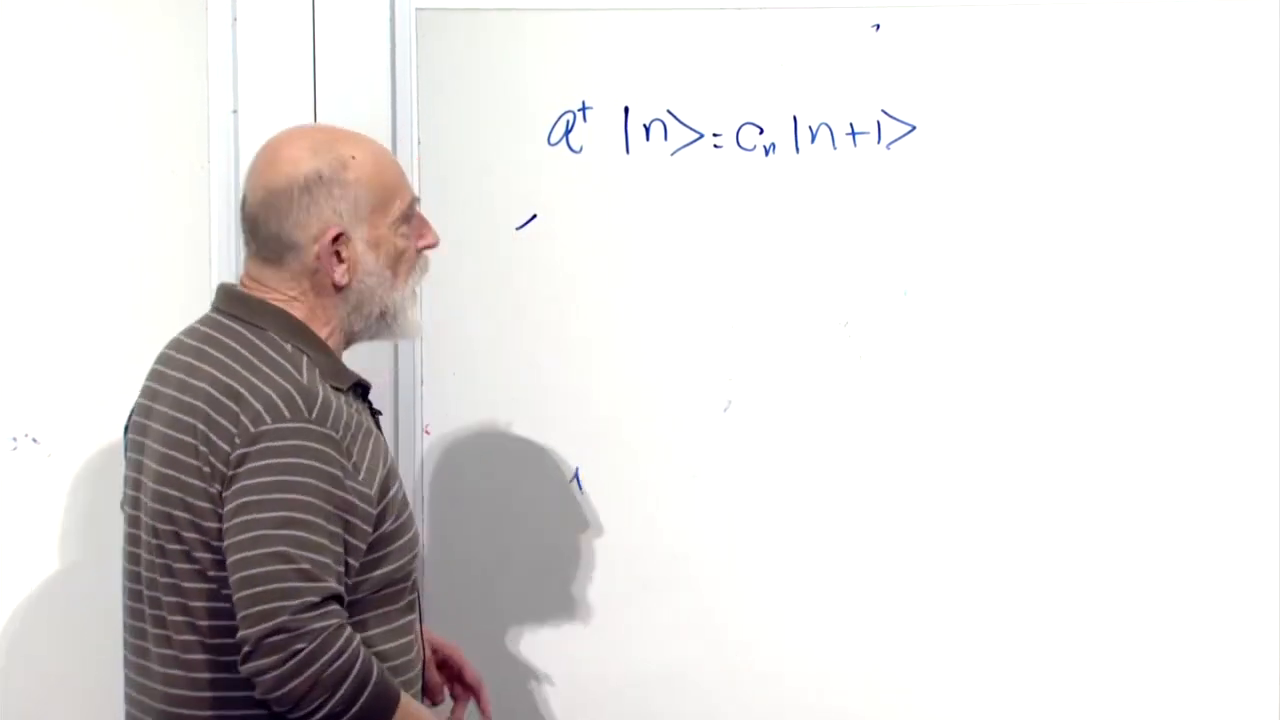
\includegraphics[width=0.9\linewidth]{lecture_06_frame_01.png}
\caption{El coeficiente de escalera se introduce antes de derivar su normalización. La ecuación de la pizarra se reproduce en la ecuación~\eqref{eq:l06-unknown-coefficient}.}
\lectureframe{00:19:38}
\end{figure}

Elijamos la convención de fase en la que \(c_n\) es real. Al tomar el conjugado hermítico, se obtiene
\begin{equation}
\langle n|a=c_n\langle n+1|.
\end{equation}
Al multiplicar las dos relaciones y usar los estados de la base normalizados,
\begin{align}
c_n^2
&=\langle n|aa^\dagger|n\rangle \\
&=\langle n|(a^\dagger a+1)|n\rangle \\
&=\langle n|(N+1)|n\rangle \\
&=n+1.
\end{align}
Por consiguiente,
\begin{equation}
a^\dagger|n\rangle=\sqrt{n+1}\,|n+1\rangle.
\label{eq:l06-raising-rule}
\end{equation}

\begin{classroomqa}
\lecturetimestamp{00:22:35}
\audiencequestion{¿Por qué se puede imponer \(\langle n+1|n+1\rangle=1\) antes de hallar \(c_n\)?}
\lecturerresponse{Los vectores propios se eligen desde el principio como una base normalizada. Su normalización no determina la normalización de \(a^\dagger|n\rangle\); la información que falta es precisamente el coeficiente \(c_n\).}
\end{classroomqa}

La regla de descenso se obtiene de la misma manera:
\begin{equation}
a|n\rangle=\sqrt n\,|n-1\rangle.
\label{eq:l06-lowering-rule}
\end{equation}
Para \(n=0\), el coeficiente se anula automáticamente, de modo que la regla incluye \(a|0\rangle=0\). Para muchos modos, el operador solo cambia el número de ocupación de su propia posición:
\begin{align}
a_i^\dagger|n_1,\ldots,n_i,\ldots\rangle
&=\sqrt{n_i+1}\,|n_1,\ldots,n_i+1,\ldots\rangle, \\
a_i|n_1,\ldots,n_i,\ldots\rangle
&=\sqrt{n_i}\,|n_1,\ldots,n_i-1,\ldots\rangle.
\label{eq:l06-multimode-ladders}
\end{align}
Las demás entradas no cambian.

\section{Una función de onda no es un campo cuántico}

Antes de definir un campo, debemos distinguirlo de la conocida función de onda. Tres contrastes organizan esta transición.

Primero, una función de onda de una partícula
\begin{equation}
\psi(x)=\langle x|\psi\rangle
\end{equation}
es una representación de un vector de estado. No es en sí misma un observable. Medimos los operadores de posición, momento, momento angular y otros; la función de onda proporciona las amplitudes a partir de las cuales se calculan las probabilidades de esos resultados.

Segundo, una función de onda de muchas partículas depende de las posiciones de todas ellas. Para dos partículas cujos vectores de posición llamaremos provisionalmente \(x\) y \(y\),
\begin{equation}
\psi(x,y)=\langle x,y|\psi\rangle.
\end{equation}
Aquí, \(x\) y \(y\) etiquetan dos partículas distintas; no son las componentes cartesianas \(x\) e \(y\) de un mismo vector de posición. Para \(N\) partículas, el estado se representa mediante
\begin{equation}
\psi(x_1,x_2,\ldots,x_N).
\end{equation}

Tercero, esta función de onda describe un número fijo de partículas. Una función de onda de quince partículas tiene quince argumentos de posición y pertenece a un espacio de Hilbert de quince partículas. Por sí sola, no describe un proceso en el que el número pase de quince a catorce o a dieciséis.

Un campo cuántico invierte estas características. Es un operador, no un estado; depende de un punto espacial \(x\) y actúa sobre un espacio de estados que contiene todos los sectores de número de partículas. La expresión ``un punto'' significa un único vector de posición libremente variable. No significa que se haya asignado a \(x\) un valor numérico concreto.

Hay una salvedad que será importante más adelante. El campo \(\Psi(x)\) que introduciremos a continuación no es hermítico, así que no es en sí mismo un observable en sentido estricto. Sus combinaciones hermíticas sí son observables. Por tanto, la afirmación provisional de que un campo es medible se precisa, no se descarta: los campos son funciones con valores de operador, y sus combinaciones hermíticas representan magnitudes medibles.

\begin{classroomqa}
\lecturetimestamp{00:36:52}
\audiencequestion{Si el campo es una función de una posición, ¿puede variar esa posición? ¿Y qué pasó con \(y\) en la función de onda de dos partículas?}
\lecturerresponse{El punto \(x\) varía por todo el espacio. ``Una posición'' significa que el operador tiene un único argumento espacial, no que ese argumento esté fijo. En \(\psi(x,y)\), los símbolos \(x\) y \(y\) designan las posiciones de dos partículas; de manera equivalente, son \(x_1\) y \(x_2\). No son dos componentes cartesianas del argumento del campo.}
\end{classroomqa}

\begin{classroomqa}
\lecturetimestamp{00:38:15}
\audiencequestion{¿Qué relación hay entre la descripción mediante una función de onda de número fijo de partículas y la descripción mediante campos? ¿Describen tipos distintos de partículas?}
\lecturerresponse{La conexión es la construcción central que aún nos falta desarrollar. Las partículas son del mismo tipo. En esta lección son bosones; los fermiones requieren un álgebra distinta.}
\end{classroomqa}

\section{Una partícula en una caja}

Volvamos por un momento a la mecánica cuántica ordinaria de una partícula. Pongamos una partícula en una caja unidimensional. Si hay una sola partícula, la distinción entre bosón y fermión es irrelevante: no hay una segunda partícula idéntica con la que comprobar el intercambio o la exclusión.

Sean
\begin{equation}
\psi_1(x),\ \psi_2(x),\ \psi_3(x),\ldots
\end{equation}
las funciones propias de la energía. El modo más bajo es la onda más suave que se anula en las paredes. El siguiente modo tiene un nodo interior, y los modos de mayor energía oscilan más rápidamente. Para un pozo cuadrado infinito ideal de anchura \(L\), una base ortonormal normalizada conveniente es
\begin{equation}
\psi_i(x)=\sqrt{\frac{2}{L}}\sin\!\left(\frac{i\pi x}{L}\right),
\qquad 0<x<L.
\label{eq:l06-box-basis}
\end{equation}
La fórmula explícita con senos es una realización estándar del esquema cualitativo de la pizarra; el argumento siguiente solo requiere un conjunto completo y ortonormal de estados de una partícula.

\begin{figure}[htbp]
\centering
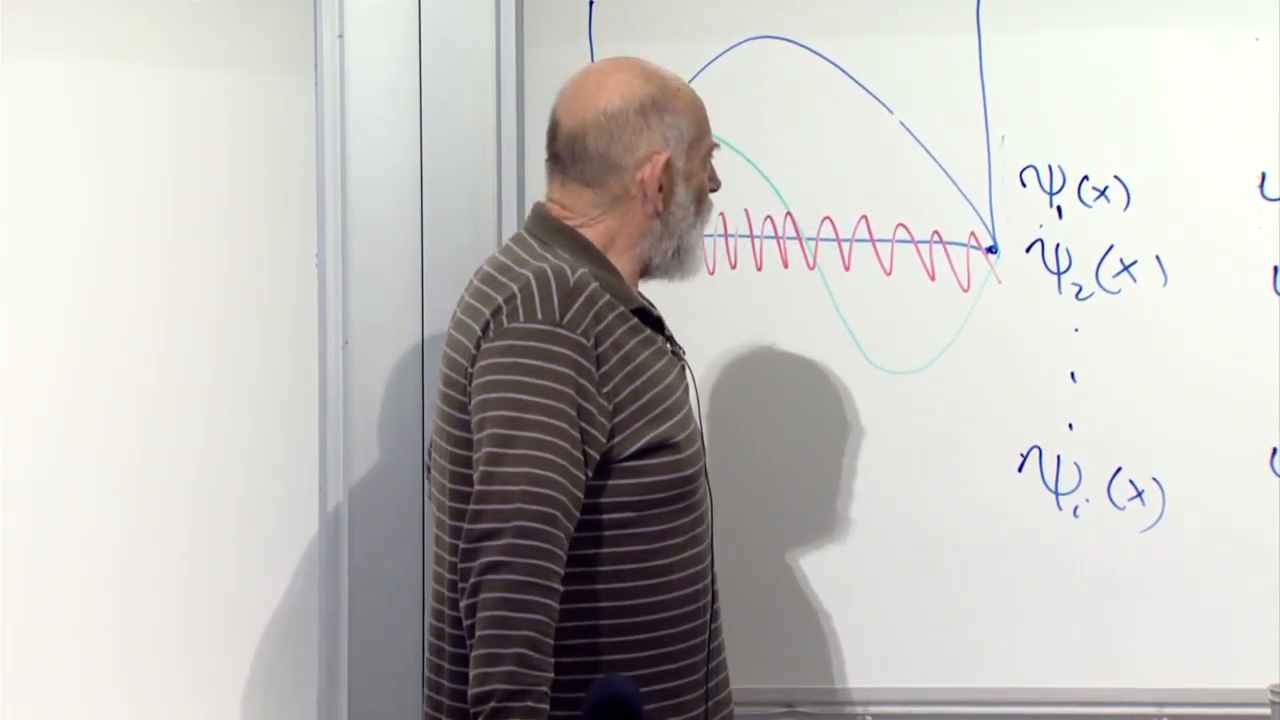
\includegraphics[width=0.9\linewidth]{lecture_06_frame_03.png}
\caption{Modos de una partícula en una caja, ordenados por energía creciente. El primer modo no tiene nodos interiores; el segundo tiene uno, y los modos superiores omitidos oscilan cada vez más rápidamente.}
\lectureframe{00:43:10}
\end{figure}

La misma estructura se puede dibujar de nuevo, sin que la oculte la pizarra en directo:
\begin{figure}[htbp]
\centering
\begin{tikzpicture}[x=1cm,y=1cm]
  \draw[thick] (0,0) -- (0,3.8);
  \draw[thick] (7,0) -- (7,3.8);
  \draw[gray!55] (0,2.75) -- (7,2.75);
  \draw[gray!55] (0,1.35) -- (7,1.35);
  \draw[blue!75!black,thick,domain=0:7,samples=120]
    plot (\x,{2.75+0.62*sin(180*\x/7)});
  \draw[teal!70!black,thick,domain=0:7,samples=120]
    plot (\x,{1.35+0.55*sin(360*\x/7)});
  \node[right] at (7.15,3.15) {$\psi_1(x)$};
  \node[right] at (7.15,1.70) {$\psi_2(x)$};
  \node at (3.5,0.45) {$\vdots\quad \psi_i(x)$};
\end{tikzpicture}
\caption{Reconstrucción limpia del esquema cualitativo de los modos de la caja. El desplazamiento vertical separa las funciones propias para facilitar su lectura; no representa una coordenada física adicional.}
\end{figure}

El índice \(i\) etiqueta un estado de una partícula, no una partícula ni el número de nodos. Para la base de la caja, resulta que \(i\) es uno más que el número de nodos interiores. Cada estado tiene una energía \(\varepsilon_i\). Siguiendo la notación de la lección, podemos escribir esta energía como \(\hbar\omega_i\) o, simplemente, como \(\omega_i\) si fijamos \(\hbar=1\).

\begin{classroomqa}
\lecturetimestamp{00:39:01}
\audiencequestion{¿Era exacta la hipótesis de independencia anterior, y podría el índice \(i\) etiquetar los estados posibles de un electrón en un átomo?}
\lecturerresponse{En la construcción de modos independientes, la conmutación entre modos distintos es exacta. El índice puede etiquetar estados atómicos de una partícula. Sin embargo, si las partículas interactúan, el Hamiltoniano sencillo de modos independientes deja de describir toda la situación.}
\end{classroomqa}

\begin{classroomqa}
\lecturetimestamp{00:40:34}
\audiencequestion{¿Es bosón la partícula de la caja?}
\lecturerresponse{Podría serlo, pero, con una sola partícula, la estadística no importa. La exclusión y el intercambio solo tienen sentido cuando hay más de una partícula idéntica.}
\end{classroomqa}

\section{De los modos de la caja al espacio de Fock}

Permitamos ahora que cualquier número de bosones idénticos ocupe la caja. Un cierto número \(n_1\) puede ocupar \(\psi_1\), otro número \(n_2\) puede ocupar \(\psi_2\), y así sucesivamente. Por tanto, un estado de la base es
\begin{equation}
|n_1,n_2,n_3,\ldots\rangle.
\end{equation}
Esta es exactamente la notación que ya usamos para muchos osciladores. La identidad es estructural: asociamos un oscilador a cada estado de una partícula e identificamos el número de excitaciones del oscilador con el número de partículas que ocupan ese estado.

Los bosones son esenciales aquí porque cada \(n_i\) puede ser cualquier entero no negativo. En el caso de los fermiones, cada estado de una partícula puede estar vacío u ocupado por una sola partícula, pero nunca ocupado por dos; por eso, el álgebra ordinaria del oscilador no se puede usar sin cambios.

Ahora podemos definir los operadores mediante su acción sobre la base de números de ocupación. El operador \(a_i^\dagger\) crea una partícula en el estado de una partícula \(i\); \(a_i\) elimina una:
\begin{align}
a_i^\dagger|n_1,\ldots,n_i,\ldots\rangle
&=\sqrt{n_i+1}\,|n_1,\ldots,n_i+1,\ldots\rangle, \\
a_i|n_1,\ldots,n_i,\ldots\rangle
&=\sqrt{n_i}\,|n_1,\ldots,n_i-1,\ldots\rangle.
\end{align}
Esto no es una analogía añadida a posteriori. Es la definición de los operadores bosónicos de creación y aniquilación en esta base. Como la base genera el espacio, la definición determina por linealidad su acción sobre cualquier estado.

\begin{classroomqa}
\lecturetimestamp{00:47:11}
\audiencequestion{¿Son \(n_1,n_2,n_3\) los estados cuánticos?}
\lecturerresponse{Las etiquetas \(1,2,3,\ldots\) identifican los estados de una partícula. Los símbolos \(n_1,n_2,n_3,\ldots\) son los números de partículas que ocupan esos estados. La principal dificultad de la notación consiste en mantener separados la etiqueta del estado y su número de ocupación.}
\end{classroomqa}

\subsection{Qué hace la raíz cuadrada}

El factor \(\sqrt{n_i+1}\) no representa una partícula adicional ni un proceso físico aparte. Da al operador la normalización y el álgebra correctas. Para un modo,
\begin{align}
a a^\dagger|n\rangle
&=a\bigl(\sqrt{n+1}\,|n+1\rangle\bigr) \\
&=(n+1)|n\rangle,
\end{align}
mientras que
\begin{equation}
a^\dagger a|n\rangle=n|n\rangle.
\end{equation}
Por tanto, su diferencia es \(|n\rangle\), como exige \([a,a^\dagger]=1\). A grandes rasgos, cada uno de los dos operadores de escalera es del orden de \(\sqrt n\), pues su producto da el operador número, que es del orden de \(n\).

\begin{classroomqa}
\lecturetimestamp{00:47:52}
\audiencequestion{¿Qué significado físico concreto tiene el factor de raíz cuadrada?}
\lecturerresponse{Su función principal es la normalización matemática. Garantiza que los estados de ocupación estén normalizados, que \(a^\dagger a\) tenga el valor propio \(n\) y que los operadores de escalera satisfagan el conmutador del oscilador. A veces, la matemática misma es el significado que hace falta.}
\end{classroomqa}

\begin{classroomqa}
\lecturetimestamp{00:52:25}
\audiencequestion{¿Se han definido los operadores de creación y aniquilación solo mediante sus propiedades y su acción sobre la base?}
\lecturerresponse{Sí. Las definiciones no tienen por qué partir de una imagen más fundamental. Su valor se comprueba por sus consecuencias. Definir la acción sobre una base completa define los operadores en todas partes, y estas definiciones reproducen las relaciones de conmutación deseadas.}
\end{classroomqa}

\begin{classroomqa}
\lecturetimestamp{00:53:22}
\audiencequestion{¿Por qué \(a_i\) hace desaparecer una partícula en vez de limitarse a trasladarla a otro estado?}
\lecturerresponse{Porque \(a_i\) está definido para disminuir la ocupación del estado \(i\). La pregunta útil no es por qué una definición es verdadera, sino por qué es útil. Lo es porque la emisión y la absorción requieren operadores que cambien el número de partículas: se crea un fotón cuando se emite radiación y se aniquila cuando se absorbe.}
\end{classroomqa}

El espacio generado por todos los estados de números de ocupación es el \emph{espacio de Fock}. Contiene el vacío, todos los estados de una partícula, todos los estados de dos partículas, y así sucesivamente, sin un límite superior fijo:
\begin{equation}
\mathcal F=\mathcal H_0\oplus\mathcal H_1\oplus\mathcal H_2\oplus\cdots.
\label{eq:l06-fock-space}
\end{equation}
La notación de suma directa hace explícito lo que no mostraba la función de onda ordinaria de \(N\) partículas: todos los sectores de número de partículas pertenecen a un mismo espacio de estados.

\begin{classroomqa}
\lecturetimestamp{00:54:56}
\audiencequestion{¿Definir los operadores sobre los vectores propios de números de ocupación determina su acción sobre vectores arbitrarios? ¿Se deducen entonces los conmutadores del oscilador?}
\lecturerresponse{Exactamente. Los vectores de ocupación forman una base, así que la linealidad extiende la definición a todo el espacio de Fock. La acción sobre esa base verifica las relaciones de conmutación bosónicas. Cada estado de una partícula está representado por un oscilador, y la ocupación de ese oscilador es el número de partículas en ese estado.}
\end{classroomqa}

\subsection{El vacío y el Hamiltoniano libre}

El vacío de Fock es el estado en el que no hay partículas en ningún estado de una partícula:
\begin{equation}
|0\rangle=|0,0,0,\ldots\rangle,
\qquad a_i|0\rangle=0.
\end{equation}
La expresión \emph{estado fundamental} puede inducir a error aquí. El estado \emph{de una partícula} de menor energía es el modo \(i=1\); en el vacío de Fock no hay ninguna partícula, ni siquiera en ese modo. Si una partícula ocupa el modo más bajo, \(a_1\) puede eliminarla y devolver el sistema al vacío.

\begin{classroomqa}
\lecturetimestamp{00:56:19}
\audiencequestion{¿Qué es el vacío en términos de números de ocupación? ¿Está ocupado el estado de una partícula de menor energía?}
\lecturerresponse{En el vacío todos los números de ocupación son cero y todos los \(a_i\) lo aniquilan. El modo de una partícula de menor energía está desocupado en el vacío. Si estuviera ocupado, su operador de aniquilación podría eliminar esa partícula.}
\end{classroomqa}

Para partículas que no interactúan, la energía total es aditiva. Si una partícula en el estado \(i\) tiene energía \(\hbar\omega_i\), entonces
\begin{align}
H
&=\sum_i \hbar\omega_i N_i \\
&=\sum_i \hbar\omega_i a_i^\dagger a_i.
\label{eq:l06-free-fock-hamiltonian}
\end{align}
Hay dos interpretaciones equivalentes. Es la suma de las energías de los osciladores, uno por cada estado de una partícula. También es la suma de las energías de una partícula, cada una multiplicada por el número de partículas que tienen esa energía.

En la notación de la teoría de campos, \(a_i^\dagger\) suele llamarse operador de creación y \(a_i\), operador de aniquilación. Las notaciones más antiguas \(a_+\) y \(a_-\) expresan lo mismo.

\section{Aclaraciones antes de introducir el campo}

Varias preguntas después de la pausa permiten distinguir este nuevo recuento mediante osciladores de una partícula ordinaria que se mueve en un potencial de oscilador.

\begin{classroomqa}
\lecturetimestamp{01:06:09}
\audiencequestion{Los niveles de energía de una partícula en una caja no están igualmente espaciados. Entonces, ¿dónde está el oscilador armónico?}
\lecturerresponse{Las energías de una partícula \(\omega_i\) no tienen por qué estar igualmente espaciadas. Sin embargo, para cada modo fijo \(i\), las energías de cero, una, dos y tres partículas que no interactúan en ese modo son \(0,\omega_i,2\omega_i,3\omega_i\). Esa escalera de ocupación es el oscilador. No debe confundirse con poner una partícula en un potencial de oscilador armónico.}
\end{classroomqa}

\begin{classroomqa}
\lecturetimestamp{01:08:38}
\audiencequestion{¿Está relacionada esta construcción con la descomposición de Fourier?}
\lecturerresponse{Está profundamente relacionada. Si la base de una partícula consta de modos de momento, las funciones de modo son senos, cosenos o exponenciales complejas, y los \(a_i\) son análogos cuánticos de los coeficientes de Fourier. Una base general no tiene por qué ser trigonométrica, pero la lógica de la expansión es la misma.}
\end{classroomqa}

\begin{classroomqa}
\lecturetimestamp{01:09:07}
\audiencequestion{¿Se asigna a todas las partículas la misma energía? ¿Se incluyen las interacciones?}
\lecturerresponse{Las partículas que ocupan el mismo estado de una partícula tienen la misma energía; las que ocupan estados distintos, por lo general, no. Por ahora, las partículas son libres: no interactúan. Las interacciones añadirían términos de energía potencial, de modo que el Hamiltoniano ya no sería únicamente la suma aditiva de la ecuación~\eqref{eq:l06-free-fock-hamiltonian}.}
\end{classroomqa}

\begin{classroomqa}
\lecturetimestamp{01:10:26}
\audiencequestion{¿Qué ocurrió con el medio cuanto de energía de punto cero de cada oscilador?}
\lecturerresponse{Es una constante aditiva del Hamiltoniano. Una constante conmuta con todos los operadores, así que no altera las ecuaciones de movimiento de Heisenberg, y las mediciones ordinarias no gravitatorias dependen de diferencias de energía. Puede importar para fines especiales, pero no afecta a la construcción que estamos desarrollando aquí.}
\end{classroomqa}

La teoría libre ya es un dispositivo de recuento de extraordinaria potencia. Permite seguir no solo muchas partículas, sino también partículas que cambian de estado, aparecen, desaparecen o existen en superposiciones con distinto número total. Los operadores son más que símbolos de recuento, porque se pueden medir combinaciones hermíticas adecuadas; aun así, el recuento es una intuición inicial útil.

\begin{classroomqa}
\lecturetimestamp{01:14:03}
\audiencequestion{¿Cuál es el origen histórico de la teoría de campos y de la teoría cuántica de campos?}
\lecturerresponse{Un breve recorrido histórico comienza con la imagen física de Faraday de los campos eléctricos y magnéticos y con las ecuaciones de Maxwell para los campos clásicos. Planck introdujo los cuantos de energía al estudiar la radiación térmica; Einstein identificó la cuantización con el propio campo electromagnético y con los cuantos de luz. Heisenberg, Pauli y, en particular, Dirac contribuyeron después a construir el marco moderno de operadores hacia finales de los 1920. La catástrofe ultravioleta y la descripción cuántica de la radiación estuvieron entre los primeros problemas decisivos. Este es un esbozo histórico, no una atribución exhaustiva de prioridades.}
\end{classroomqa}

El hilo histórico también explica por qué los osciladores vuelven una y otra vez. La radiación clásica en una cavidad se descompone en modos normales. Al cuantizar esos modos, sus números de excitación se convierten en números de fotones. Los cuantos matemáticos que ocupan los modos pasan a ser partículas físicas.

\section{El operador de campo bosónico}

Sea \(\{\psi_i(x)\}\) una base completa y ortonormal de funciones de onda de una partícula. Definamos
\begin{equation}
\boxed{\Psi(x)=\sum_i a_i\,\psi_i(x)}
\label{eq:l06-field-annihilation}
\end{equation}
y su conjugado hermítico
\begin{equation}
\boxed{\Psi^\dagger(x)=\sum_i a_i^\dagger\,\psi_i^*(x)}.
\label{eq:l06-field-creation}
\end{equation}

\begin{figure}[htbp]
\centering
\includegraphics[width=0.9\linewidth]{lecture_06_frame_04.png}
\caption{Expansiones completas en modos del campo de aniquilación y de su conjugado hermítico. Las ecuaciones~\eqref{eq:l06-field-annihilation} y \eqref{eq:l06-field-creation} conservan en la composición tipográfica la misma estructura de operadores y conjugación compleja.}
\lectureframe{01:25:15}
\end{figure}

Para cualquier posición fija \(x\), cada \(\psi_i(x)\) es un número complejo ordinario. Todo el contenido de operador reside en \(a_i\) y \(a_i^\dagger\). Al variar \(x\), obtenemos un operador distinto en cada punto del espacio. Este es el sentido preciso en que \(\Psi\) es una función con valores de operador.

Si las funciones de la base son ondas planas, las ecuaciones~\eqref{eq:l06-field-annihilation} y \eqref{eq:l06-field-creation} son expansiones de Fourier cuánticas: los coeficientes de Fourier clásicos se han convertido en operadores. En una caja, la base puede constar, en cambio, de las funciones seno de la ecuación~\eqref{eq:l06-box-basis}. Sirve cualquier base completa y ortonormal de una partícula.

Ni \(\Psi\) ni \(\Psi^\dagger\) es hermítico. Se pueden construir campos observables a partir de combinaciones hermíticas como
\begin{equation}
\Psi(x)+\Psi^\dagger(x),
\qquad
i\bigl(\Psi^\dagger(x)-\Psi(x)\bigr),
\end{equation}
y más adelante se construirán densidades observables a partir de productos como \(\Psi^\dagger(x)\Psi(x)\). La tarea inmediata es entender primero qué hacen los dos campos básicos.

\begin{classroomqa}
\lecturetimestamp{01:23:14}
\audiencequestion{¿Cómo puede el miembro de la izquierda ser un operador si las funciones de modo de la derecha son funciones de onda ordinarias?}
\lecturerresponse{Las funciones \(\psi_i(x)\) son números una vez elegido \(x\). Los factores \(a_i\) son operadores. El producto de un número y un operador sigue siendo un operador, así que la suma también lo es. Al variar \(x\) se obtiene la familia completa de operadores.}
\end{classroomqa}

\section{Qué hace el campo}

El campo de aniquilación aniquila el vacío de inmediato:
\begin{equation}
\Psi(x)|0\rangle
=\sum_i\psi_i(x)a_i|0\rangle
=0.
\label{eq:l06-field-kills-vacuum}
\end{equation}
El campo de creación hace algo mucho más revelador.

Sea \(|i\rangle\) el estado de una partícula cuya función de onda es
\begin{equation}
\langle x|i\rangle=\psi_i(x).
\end{equation}
La completitud de la base de una partícula da
\begin{equation}
\sum_i|i\rangle\langle i|=1.
\label{eq:l06-completeness}
\end{equation}
Apliquemos esta identidad a un autoestado de posición:
\begin{align}
|x\rangle
&=\sum_i|i\rangle\langle i|x\rangle \\
&=\sum_i\psi_i^*(x)|i\rangle.
\label{eq:l06-position-expansion}
\end{align}
En el lenguaje de Fock, un estado de modo de una partícula es
\begin{equation}
|i\rangle=a_i^\dagger|0\rangle.
\end{equation}
Al sustituirlo en la ecuación~\eqref{eq:l06-position-expansion},
\begin{align}
|x\rangle
&=\sum_i\psi_i^*(x)a_i^\dagger|0\rangle \\
&=\Psi^\dagger(x)|0\rangle.
\label{eq:l06-local-creation}
\end{align}
Así, \(\Psi^\dagger(x)\) crea una partícula localizada en \(x\), mientras que \(\Psi(x)\) elimina allí una partícula. Un autoestado de posición está localizado mediante una delta de Dirac y es un estado generalizado no normalizable; para obtener una partícula localizada física, se integra el campo contra un paquete de ondas normalizable.\editorialnote{La lección emplea el lenguaje ideal de los autoestados de posición. La salvedad sobre el paquete de ondas recoge el significado matemático estándar sin cambiar el argumento.}

\begin{classroomqa}
\lecturetimestamp{01:36:26}
\audiencequestion{¿Qué información especifica qué tipo de partícula se crea? ¿Está el estado en \(x\) localizado mediante una delta de Dirac?}
\lecturerresponse{Se asigna un campo distinto a cada especie de partícula, así que la identidad de la partícula viene determinada por el campo que se use. El argumento \(x\) especifica dónde se crea. En la base ideal de posición, el estado creado tiene localización delta de Dirac.}
\end{classroomqa}

Entre las especies bosónicas se cuentan los fotones, los gravitones, los bosones de Higgs y los gluones, aunque los campos realistas también llevan índices internos. Incluso los fotones requieren etiquetas de polarización. La notación simplificada de campo escalar omite esas etiquetas adicionales para que el principio de creación siga siendo visible.

\subsection{El vacío no es el vector cero}

La ecuación
\begin{equation}
\Psi(x)|0\rangle=0
\end{equation}
contiene dos objetos muy distintos que se denotan con cero. El ket \(|0\rangle\) es el vacío: un estado físico normalizado que satisface
\begin{equation}
\langle0|0\rangle=1.
\end{equation}
El resultado de la derecha es el vector cero. Su norma es cero; no se puede normalizar y no representa un estado físico.

La diferencia se hace patente al sumar. Sumar el vector cero a un estado de una partícula no cambia nada. Sumar el vacío a un estado de una partícula produce una superposición genuina de sectores con distinto número de partículas. Con coeficientes normalizados,
\begin{equation}
|\chi\rangle=\frac{1}{\sqrt2}\bigl(|0\rangle+|1\rangle\bigr)
\end{equation}
asigna probabilidades iguales a cero y una partícula. No es lo mismo que \(|1\rangle\).

\begin{classroomqa}
\lecturetimestamp{01:37:23}
\audiencequestion{Si no hay ninguna partícula en \(x\), ¿\(\Psi(x)\) simplemente no hace nada? ¿Qué significa que el resultado sea cero?}
\lecturerresponse{No devuelve el estado original. Devuelve el vector nulo. El vacío es un estado normalizado que describe el espacio vacío; el vector nulo tiene longitud cero y no describe ningún estado físico. Cualquier operador que actúe sobre el vector nulo devuelve el vector nulo.}
\end{classroomqa}

\begin{classroomqa}
\lecturetimestamp{01:39:00}
\audiencequestion{¿Qué ocurre si se suma el vacío, en lugar del vector nulo, a un estado de una partícula?}
\lecturerresponse{Se obtiene una superposición con amplitudes correspondientes a distintos números de partículas. En cambio, sumar el vector nulo deja intacto el estado de una partícula. El símbolo \(|0\rangle\) designa la ocupación nula; no significa vector nulo.}
\end{classroomqa}

\begin{classroomqa}
\lecturetimestamp{01:41:56}
\audiencequestion{¿Importa el orden de una función modal y su operador de creación o aniquilación en la expansión del campo? ¿Las funciones modales son complejas?}
\lecturerresponse{La función modal es un número ordinario y, por tanto, conmuta con todos los operadores, así que el orden no importa. En general, las funciones modales pueden ser complejas; que una base elegida sea real o compleja depende del problema de una partícula de Schr\"odinger Schrödinger.}
\end{classroomqa}

\subsection{Dos partículas y la aparición de la simetría bosónica}

Para crear una partícula en \(x\) y otra en \(y\), se actúa dos veces:
\begin{equation}
|x,y\rangle
=\Psi^\dagger(y)\Psi^\dagger(x)|0\rangle.
\label{eq:l06-two-particle-state}
\end{equation}
Los puntos pueden coincidir o ser distintos. Como los operadores de creación subyacentes conmutan,
\begin{align}
[\Psi^\dagger(x),\Psi^\dagger(y)]
&=\sum_{i,j}\psi_i^*(x)\psi_j^*(y)
[a_i^\dagger,a_j^\dagger] \\
&=0.
\end{align}
Se sigue que
\begin{equation}
\Psi^\dagger(y)\Psi^\dagger(x)|0\rangle
=\Psi^\dagger(x)\Psi^\dagger(y)|0\rangle.
\label{eq:l06-boson-exchange}
\end{equation}
Intercambiar el orden de las dos partículas no cambia nada. Esta es precisamente la simetría de intercambio bosónica. Por tanto, podríamos haber partido del álgebra del oscilador y \emph{deducido} que las partículas construidas con operadores de creación que conmutan son bosones. Para los fermiones se necesitarán, en cambio, operadores que anticonmuten.

\begin{classroomqa}
\lecturetimestamp{01:42:37}
\audiencequestion{¿Cómo se añade una segunda partícula al estado de una partícula?}
\lecturerresponse{Se aplica otro campo de creación. Para añadirla en \(y\), se actúa con \(\Psi^\dagger(y)\) a la izquierda de \(\Psi^\dagger(x)\). El resultado es el estado de dos partículas de la ecuación~\eqref{eq:l06-two-particle-state}.}
\end{classroomqa}

\begin{classroomqa}
\lecturetimestamp{01:46:04}
\audiencequestion{¿La conmutatividad de los dos campos de creación equivale plenamente a simetrizar el estado de dos partículas?}
\lecturerresponse{Sí. Hace que el estado con una partícula en \(x\) y otra en \(y\) sea idéntico al estado que se obtiene al intercambiar las etiquetas. Esta es la propiedad de intercambio que define a los bosones idénticos.}
\end{classroomqa}

\begin{classroomqa}
\lecturetimestamp{01:46:32}
\audiencequestion{¿Significa esto que las partículas en \(x\) y \(y\) deben ser bosones del mismo tipo?}
\lecturerresponse{Sí. Los argumentos \(x\) y \(y\) son posiciones, mientras que un campo describe una especie. Las distintas especies y las etiquetas adicionales, como las dos polarizaciones del fotón, requieren componentes de campo diferentes.}
\end{classroomqa}

\section{Por qué importa que el número de partículas pueda variar}

Si un problema contuviera exactamente 37 partículas para siempre, el lenguaje de campos sería una herramienta opcional de contabilidad. Su verdadera utilidad aparece cuando las partículas pueden emitirse y absorberse, y sobre todo cuando el propio número de partículas es una variable cuántica. El espacio de Fock permite estados de la forma
\begin{equation}
|\Phi\rangle
=c_0|0\rangle+c_1|1\rangle+c_2|2\rangle+\cdots,
\qquad
\sum_{n=0}^{\infty}|c_n|^2=1.
\end{equation}
Un campo láser es un ejemplo importante: en general, no es un estado con un número de fotones definido, sino una superposición de muchos sectores de número.

El vínculo entre partículas y campos ya es explícito. Los operadores modales cuentan partículas y modifican su número en los estados propios de la energía; el campo combina esos operadores con un conjunto completo de funciones de onda para que se puedan crear o eliminar partículas en posiciones determinadas. El álgebra de los osciladores armónicos se ha convertido en el lenguaje elemental de un campo cuántico bosónico.

\chapter{De las partículas a un campo cuántico sencillo}

Construyamos de nuevo el campo cuántico sencillo, pero desde un ángulo algo distinto. Hay dos caminos para llegar a la teoría cuántica de campos. Podemos partir de las partículas y descubrir por qué un campo es el lenguaje natural para describirlas, o partir de un campo ondulatorio y descubrir por qué sus excitaciones aparecen en cuantos. Ambos caminos son útiles. Aquí seguiremos el primero.

La mecánica cuántica ordinaria puede describir una partícula, dos partículas o cualquier otro número fijo. La naturaleza no respeta esa restricción. El número de fotones en una habitación cambia cada vez que las luces emiten o absorben radiación. Las partículas inestables se desintegran. Por ejemplo, en la desintegración beta,
\begin{equation}
n\longrightarrow p+e^-+\bar{\nu}_e,
\end{equation}
cambian a la vez las poblaciones de varias especies de partículas. Por eso queremos una mecánica cuántica lo bastante amplia para incluir todos los números de ocupación posibles y, con el tiempo, los procesos que permiten pasar de unos a otros.

Por ahora simplificaremos drásticamente. Hay una sola especie de partículas no relativistas. Primero ampliaremos su espacio de estados para que pueda contener cualquier número de partículas y solo después hablaremos de más especies, relatividad, dispersión y desintegración. Ninguna de las matemáticas es especialmente difícil, pero el cambio de perspectiva es abstracto. Conviene avanzar despacio para que la notación no oculte la idea.

\section{El punto de partida: una partícula}

Empecemos con una sola partícula en el estado \(|\psi\rangle\). Su función de onda en el espacio de posiciones es
\begin{equation}
\psi(x)=\langle x|\psi\rangle.
\label{eq:l07-wavefunction}
\end{equation}
Esta \(\psi\) minúscula es una función ordinaria con valores complejos. Todavía no es un campo cuántico ni un operador que actúe sobre un espacio de estados de muchas partículas.

La regla de Born dice que
\begin{equation}
\rho_\psi(x)=|\psi(x)|^2=\psi^*(x)\psi(x)
\label{eq:l07-born-density}
\end{equation}
es la densidad de probabilidad de encontrar la partícula en \(x\). Para un estado normalizado,
\begin{equation}
\int dx\,\psi^*(x)\psi(x)=1.
\label{eq:l07-one-particle-normalization}
\end{equation}
El miembro derecho es la probabilidad total. Como este problema contiene exactamente una partícula, también resulta ser el número de partículas. Esa coincidencia será una pista útil, aunque aquí sea trivial.

\begin{classroomqa}
\lecturetimestamp{00:09:13}
\audiencequestion{¿Por qué debe tener la densidad de probabilidad la forma \(\psi^*(x)\psi(x)\)?}
\lecturerresponse{Esa es la regla de Born, uno de los postulados de la mecánica cuántica. La amplitud correspondiente al resultado de posición \(x\) es \(\langle x|\psi\rangle\); la densidad de probabilidad es su módulo al cuadrado. No se deriva de la construcción de campos que veremos más adelante.}
\end{classroomqa}

\section{Modos, ortogonalidad y completitud}

Hay muchas bases útiles para el espacio de Hilbert de una partícula. Los estados propios de posición forman una base. Los estados propios de cualquier operador hermítico forman otra, con las salvedades habituales para los espectros degenerados y continuos. Como pronto nos interesará la energía, elijamos un conjunto completo y ortonormal de estados propios de energía de una partícula:
\begin{equation}
|1\rangle,\ |2\rangle,\ldots,
\qquad
\psi_i(x)=\langle x|i\rangle.
\end{equation}

Una partícula en una caja permite concretar el índice \(i\). La función de onda del estado fundamental no tiene nodos interiores; la del siguiente estado tiene uno, y las de los estados superiores oscilan con más rapidez. En esencia, son ondas sinusoidales de un pozo cuadrado infinito ideal.

\begin{figure}[htbp]
\centering
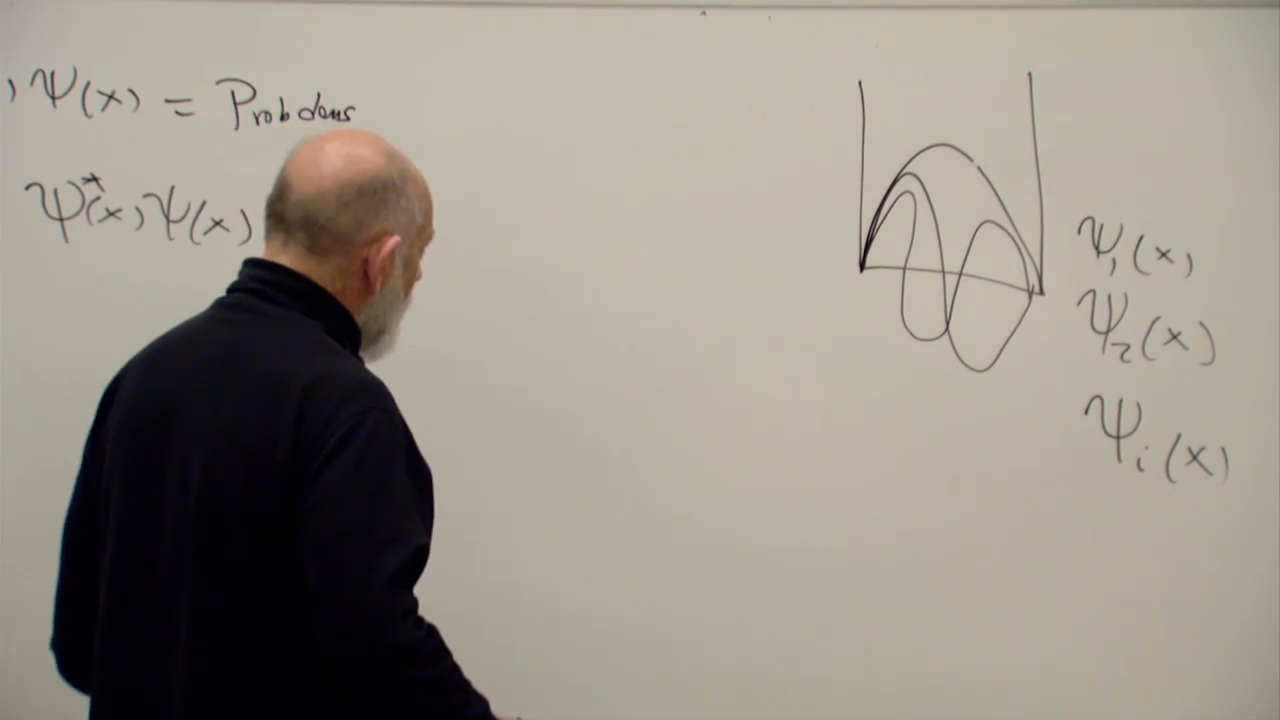
\includegraphics[width=0.94\linewidth]{lecture_07_frame_01.png}
\caption{Los modos de la caja en la pizarra de la clase. A la izquierda se ven restos de la densidad de Born de una partícula y de su normalización; a la derecha, el pozo muestra \(\psi_1(x)\), \(\psi_2(x)\) y la etiqueta general \(\psi_i(x)\).}
\lectureframe{00:08:25}
\end{figure}

La misma estructura de modos puede separarse de lo que oculta la pizarra en directo:
\begin{figure}[htbp]
\centering
\begin{tikzpicture}[x=1cm,y=1cm]
  \draw[thick] (0,0) -- (0,4.0);
  \draw[thick] (7,0) -- (7,4.0);
  \draw[gray!55] (0,2.85) -- (7,2.85);
  \draw[gray!55] (0,1.35) -- (7,1.35);
  \draw[blue!75!black,thick,domain=0:7,samples=120]
    plot (\x,{2.85+0.62*sin(180*\x/7)});
  \draw[teal!70!black,thick,domain=0:7,samples=120]
    plot (\x,{1.35+0.55*sin(360*\x/7)});
  \node[right] at (7.15,3.20) {$\psi_1(x)$};
  \node[right] at (7.15,1.70) {$\psi_2(x)$};
  \node at (3.5,0.38) {$\vdots\quad\psi_i(x)$};
\end{tikzpicture}
\caption{Una reconstrucción limpia del esquema cualitativo de la caja. Los desplazamientos verticales solo separan las dos funciones de onda para mostrarlas.}
\end{figure}

La ortonormalidad se expresa como
\begin{equation}
\int dx\,\psi_i^*(x)\psi_j(x)=\delta_{ij}.
\label{eq:l07-orthonormality}
\end{equation}
Si \(i=j\), el estado está normalizado y la integral vale uno. Si \(i\ne j\), los dos estados son ortogonales y la integral se anula.

La completitud es la afirmación, igualmente importante,
\begin{equation}
\sum_i |i\rangle\langle i|=\mathbf 1.
\label{eq:l07-resolution}
\end{equation}
Cada \(|i\rangle\langle i|\) proyecta sobre una dirección de la base; la suma sobre la base completa es la identidad. Al actuar sobre un vector arbitrario, simplemente lo descompone en sus componentes y luego lo recompone.

Ahora intercalemos la Ecuación~\eqref{eq:l07-resolution} entre dos estados de posición:
\begin{align}
\langle y|x\rangle
&=\sum_i\langle y|i\rangle\langle i|x\rangle \\
&=\sum_i\psi_i(y)\psi_i^*(x) \\
&=\delta(y-x).
\label{eq:l07-position-completeness}
\end{align}
El asterisco debe ir en el factor cuyo orden bra-ket es \(\langle i|x\rangle\). Invertir \(x\) y \(y\) da la forma equivalente conjugada compleja. Así, toda base completa y ortonormal proporciona una representación de la delta de Dirac. Las funciones seno, coseno, las funciones de onda del oscilador y las funciones propias de energía cumplen todas la misma función.

\begin{classroomqa}
\lecturetimestamp{00:13:43}
\audiencequestion{¿Debe llevar conjugación compleja la segunda función de onda de la suma de completitud?}
\lecturerresponse{Sí. Con el orden \(\langle y|i\rangle\langle i|x\rangle\), los factores son \(\psi_i(y)\psi_i^*(x)\). Mantener visible el orden bra-ket evita tener que adivinar dónde va el asterisco o colocarlo mal.}
\end{classroomqa}

Estas son las matemáticas de una partícula que necesitaremos. Ahora cambiaremos el espacio de estados.

\section{El espacio de Fock como espacio de estados más amplio}

Para muchas partículas idénticas, una base conveniente registra cuántas partículas ocupan cada modo de una partícula:
\begin{equation}
|n_1,n_2,n_3,\ldots\rangle.
\label{eq:l07-fock-basis}
\end{equation}
El entero \(n_i\) es el número de ocupación del modo \(i\). Este ket no es un estado de una partícula escrito con una notación rebuscada. Pertenece a un espacio de Hilbert más amplio que contiene el sector de cero partículas, todos los estados de una partícula, todos los estados de dos partículas, y así sucesivamente. Ese espacio más amplio se llama espacio de Fock.

Para cambiar las ocupaciones, introduzcamos para cada modo un operador de creación y otro de aniquilación:
\begin{equation}
a_i^\dagger,\qquad a_i.
\end{equation}
El primero añade una partícula al modo \(i\), mientras que el segundo elimina una. En esta etapa, el lenguaje del oscilador armónico es un recurso para llevar la cuenta: no tiene por qué haber un resorte que oscile literalmente. El álgebra del oscilador nos proporciona exactamente las herramientas necesarias para aumentar y disminuir los números de ocupación.

El operador número del modo es
\begin{equation}
\begin{aligned}
N_i&=a_i^\dagger a_i,\\
N_i|n_1,\ldots,n_i,\ldots\rangle
&=n_i|n_1,\ldots,n_i,\ldots\rangle.
\end{aligned}
\end{equation}
El vacío es
\begin{equation}
|0\rangle\equiv|0,0,0,\ldots\rangle,
\qquad
a_i|0\rangle=0
\quad\text{for every }i.
\label{eq:l07-vacuum}
\end{equation}
Por tanto, un estado de una partícula en el modo \(i\) es
\begin{equation}
|i\rangle=a_i^\dagger|0\rangle.
\label{eq:l07-mode-created}
\end{equation}
Ahora el mismo símbolo \(|i\rangle\) puede interpretarse como un vector de la base de una partícula o como ese vector incorporado al sector de una partícula del espacio de Fock. La incorporación está dada por la Ecuación~\eqref{eq:l07-mode-created}; el contexto indica de qué espacio se está hablando.

\section{Reunir los modos en un campo}

Definamos los campos de aniquilación y creación mediante
\begin{equation}
\Psi(x)=\sum_i \psi_i(x)a_i,
\qquad
\Psi^\dagger(x)=\sum_i \psi_i^*(x)a_i^\dagger.
\label{eq:l07-field-expansion}
\end{equation}
La mayúscula importa. Las funciones \(\psi_i(x)\) minúsculas son números complejos; la \(\Psi(x)\) mayúscula es un operador sobre el espacio de Fock. En cada punto espacial \(x\), la Ecuación~\eqref{eq:l07-field-expansion} da una combinación lineal distinta de los operadores de modo. Eso es lo que significa que una función de la posición tome valores que son operadores.

Para partículas libres, las funciones de modo pueden ser ondas planas \(e^{ikx}\). En ese caso, la Ecuación~\eqref{eq:l07-field-expansion} es una expansión de Fourier, salvo que sus coeficientes de Fourier son operadores y no números. La terminología antigua llama \(c\)-números a los números complejos ordinarios y \(q\)-números a los operadores cuánticos. Las funciones de modo son \(c\)-números y conmutan con todo; \(a_i\) y \(a_i^\dagger\) son los que tienen carácter de operador.

Ni \(\Psi\) ni \(\Psi^\dagger\) es hermítico. Sus adjuntos son el uno del otro. Las dos combinaciones
\begin{equation}
\Psi+\Psi^\dagger,
\qquad
i(\Psi^\dagger-\Psi)
\label{eq:l07-hermitian-combinations}
\end{equation}
son hermíticas y pueden representar observables. Por ahora, sin embargo, los campos son más útiles como herramientas para crear, aniquilar y contar partículas localmente.

\begin{classroomqa}
\lecturetimestamp{00:21:05}
\audiencequestion{¿Qué significa que un operador dependa de \(x\)?}
\lecturerresponse{Significa que cada valor de \(x\) selecciona un operador distinto. La dependencia espacial está en las funciones de modo ordinarias, mientras que cada combinación lineal resultante actúa sobre el mismo espacio de Fock.}
\end{classroomqa}

\section{Qué hace el campo de creación}

Una definición se vuelve útil cuando preguntamos qué hace. Partamos de un estado propio de posición en el sector de una partícula e insertemos la resolución de la identidad:
\begin{align}
|x\rangle
&=\sum_i |i\rangle\langle i|x\rangle \\
&=\sum_i a_i^\dagger|0\rangle\,\psi_i^*(x) \\
&=\Psi^\dagger(x)|0\rangle.
\label{eq:l07-local-creation}
\end{align}
Así, \(a_i^\dagger\) crea una partícula en el modo definido \(i\), mientras que \(\Psi^\dagger(x)\) crea una partícula localizada en \(x\). En la base idealizada de posición, esa localización es una distribución; una preparación física usaría un paquete de ondas estrecho, pero el significado algebraico es el mismo.

\begin{classroomqa}
\lecturetimestamp{00:24:48}
\audiencequestion{¿Es \(\sum_i|i\rangle\langle i|\) un proyector?}
\lecturerresponse{Cada término es un proyector sobre un estado de la base. La suma completa es la propia identidad y se llama resolución de la identidad. Insertarla no cambia ningún estado, pero hace explícitas las componentes del estado en la base elegida.}
\end{classroomqa}

La Ecuación~\eqref{eq:l07-local-creation} ofrece la primera interpretación directa del campo en términos de partículas. No nos hemos limitado a asignar una etiqueta espacial a un operador abstracto. Hemos construido la operación que crea una partícula en ese punto del espacio.

\begin{classroomqa}
\lecturetimestamp{00:28:20}
\audiencequestion{¿Debe marcarse el campo de creación en el espacio de posiciones con un asterisco o con una daga?}
\lecturerresponse{Para el adjunto de un operador se usa una daga. Los asteriscos indican la conjugación compleja de las funciones de onda ordinarias \(\psi_i(x)\); las dagas van en \(a_i^\dagger\) y \(\Psi^\dagger(x)\).}
\end{classroomqa}

\begin{classroomqa}
\lecturetimestamp{00:28:36}
\audiencequestion{¿Se pueden mover los operadores de creación a través de las funciones de onda en la expansión en modos?}
\lecturerresponse{Sí. Los \(\psi_i(x)\) son \(c\)-números, así que conmutan con todos los operadores. Solo hay que tener cuidado al cambiar el orden de operadores que no conmutan, como \(a_i\) y \(a_j^\dagger\).}
\end{classroomqa}

\section{De la densidad de probabilidad a la densidad de partículas}

Juguemos ahora con el campo. La primera expresión natural es
\begin{equation}
\int dx\,\Psi^\dagger(x)\Psi(x).
\end{equation}
Se parece a la integral de normalización de una partícula, pero ahora sus factores son operadores. Insertemos las expansiones en modos sin cambiar su orden:
\begin{align}
\int dx\,\Psi^\dagger(x)\Psi(x)
&=\int dx
\left(\sum_i a_i^\dagger\psi_i^*(x)\right)\\
&\qquad\times\left(\sum_j a_j\psi_j(x)\right) \\
&=\sum_{i,j}a_i^\dagger a_j
\int dx\,\psi_i^*(x)\psi_j(x) \\
&=\sum_{i,j}a_i^\dagger a_j\,\delta_{ij} \\
&=\sum_i a_i^\dagger a_i.
\label{eq:l07-number-derivation}
\end{align}
Por tanto, el operador número total es
\begin{equation}
N=\sum_i N_i
=\int dx\,\Psi^\dagger(x)\Psi(x).
\label{eq:l07-total-number}
\end{equation}
En los estados que estamos considerando, las excitaciones de energía finita tienen ocupaciones que decaen a energías de modo suficientemente altas, de modo que este total suele ser finito aunque la lista de modos posibles sea infinita.

El integrando es el operador de densidad local de partículas:
\begin{equation}
n(x)=\Psi^\dagger(x)\Psi(x).
\label{eq:l07-density}
\end{equation}
En rigor, no se mide la densidad en un punto matemático. Para una región pequeña \(R\), se mide
\begin{equation}
N_R=\int_R dx\,n(x),
\label{eq:l07-regional-number}
\end{equation}
el número de partículas en esa región. Como cualquier observable cuántico, \(N_R\) no tiene por qué tener un valor definido en un estado arbitrario. Preparaciones repetidas pueden dar resultados distintos.

\begin{classroomqa}
\lecturetimestamp{00:36:27}
\audiencequestion{¿Es \(\Psi^\dagger(x)\Psi(x)\) la densidad de probabilidad de muchas partículas?}
\lecturerresponse{Su significado directo es la densidad de partículas. En general, una amplitud de probabilidad de muchas partículas depende de todas las coordenadas de las partículas. En cambio, al integrar el bilineal local sobre una región pequeña, se cuentan las partículas que hay en ella.}
\end{classroomqa}

\begin{classroomqa}
\lecturetimestamp{00:38:28}
\audiencequestion{¿Actúan los operadores \(a_i\) y \(a_i^\dagger\) solo sobre vectores de estado y no sobre las funciones de onda de una partícula?}
\lecturerresponse{Sí. Actúan sobre estados del espacio de Fock, como \(|n_1,n_2,\ldots\rangle\). Las funciones de modo de una partícula que los multiplican son números ordinarios y no son los objetos sobre los que actúan estos operadores escalera.}
\end{classroomqa}

Los kets de ocupación forman una base, no el estado más general. Se pueden superponer, incluso en superposiciones en las que el mismo número total se distribuye de distintas maneras entre los modos. Para especies neutras como los fotones, también se pueden superponer distintos números totales de partículas. El operador de la Ecuación~\eqref{eq:l07-regional-number} conserva el mismo significado operacional en todos esos estados.

\begin{classroomqa}
\lecturetimestamp{00:40:01}
\audiencequestion{Si se divide la densidad de partículas por el número total, ¿se obtiene la densidad de probabilidad de encontrar una partícula en \(x\)?}
\lecturerresponse{En un sistema de población grande con \(N\) fijo, \(N_R/N\) es una frecuencia relativa y suele representar muy bien una probabilidad de una partícula. No es una identidad entre operadores que equipare el resultado de una medición con una probabilidad. En una imagen de partículas independientes, el recuento medido fluctúa, típicamente en una cantidad del orden de \(\sqrt N\), y una medición excepcional puede diferir mucho de la probabilidad aunque sea poco probable.}
\end{classroomqa}

\begin{classroomqa}
\lecturetimestamp{00:42:25}
\audiencequestion{¿Qué ocurre con la conservación de la carga en una superposición de un estado con un electrón y otro sin electrones?}
\lecturerresponse{Esa no es la clase de superposición que se usa en un sector cerrado de carga eléctrica fija. Se pueden superponer distribuciones distintas que tengan la misma carga total. Los fotones no tienen carga eléctrica, así que los distintos sectores de número de fotones no plantean ese problema. Los números de electrones y positrones también pueden cambiar a la vez mientras la carga neta permanece fija.}
\end{classroomqa}

\section{La energía de partículas independientes}

El siguiente observable es la energía. Empecemos por restringirnos a partículas que no interactúan entre sí. Esta suele ser una buena aproximación en un sistema diluido. En principio, incluso los fotones interactúan mediante procesos de orden superior, pero la radiación habitual en el laboratorio es lo bastante diluida como para que la descripción de partículas independientes sea excelente.

Sea \(\omega_i\) la energía de una partícula en el modo \(i\), con \(\hbar=1\). Un modo es un estado de una partícula. Entonces, el Hamiltoniano total es
\begin{equation}
H=\sum_i\omega_i N_i
=\sum_i\omega_i a_i^\dagger a_i.
\label{eq:l07-mode-hamiltonian}
\end{equation}
Cada modo ocupado aporta su energía de una partícula una vez por cada partícula.

\begin{classroomqa}
\lecturetimestamp{00:48:16}
\audiencequestion{¿Es \(\omega_i\) una función de la posición?}
\lecturerresponse{No. Es el autovalor de energía asociado al modo \(i\). La función \(\psi_i(x)\) depende de la posición; \(\omega_i\) depende del nivel de energía elegido.}
\end{classroomqa}

Los valores \(\omega_i\) se determinan mediante la ecuación de Schrödinger independiente del tiempo para una partícula. Definamos
\begin{equation}
h=-\frac{\nabla^2}{2m}+V(x).
\label{eq:l07-one-particle-h}
\end{equation}
Entonces,
\begin{equation}
h\psi_i(x)=\omega_i\psi_i(x).
\label{eq:l07-schrodinger-eigenvalue}
\end{equation}
En una dimensión, el operador momento es \(p=-i\partial_x\) y \(p^2/(2m)\) pasa a ser \(-\partial_x^2/(2m)\). En tres dimensiones, las tres derivadas segundas se combinan en \(-\nabla^2/(2m)\).

\begin{figure}[htbp]
\centering
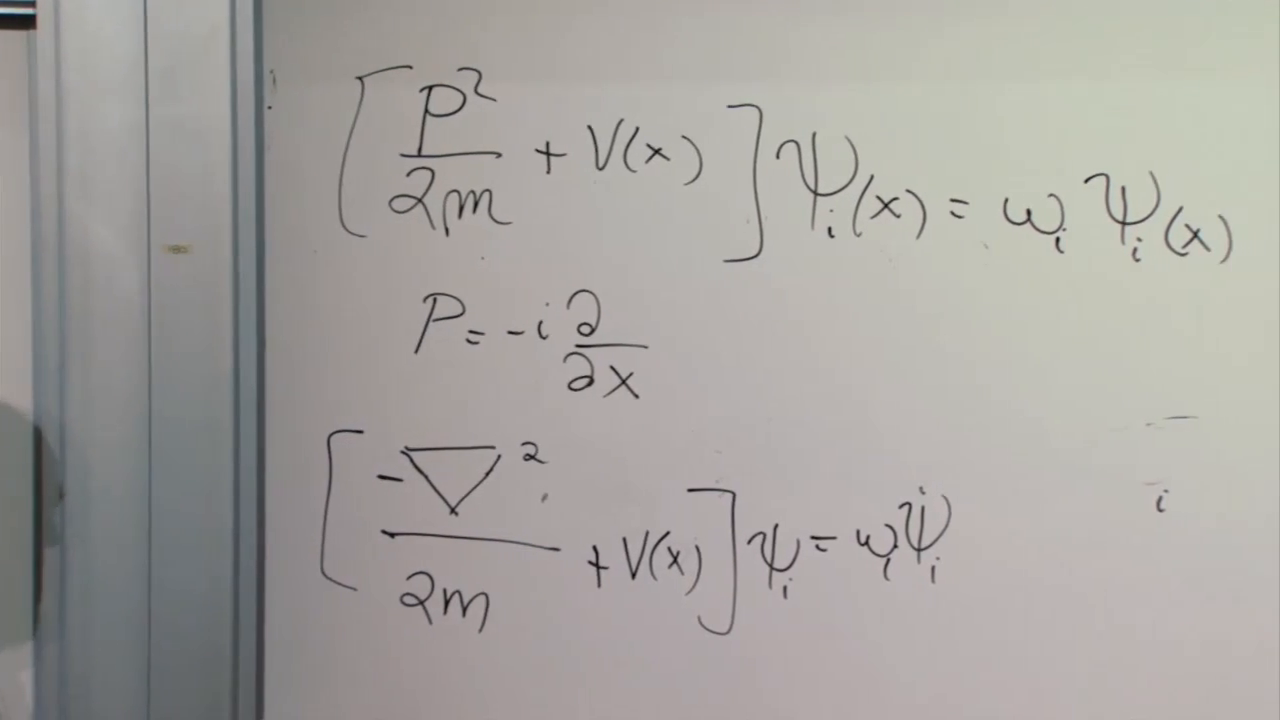
\includegraphics[width=0.94\linewidth]{lecture_07_frame_02.png}
\caption{El paso en la pizarra de \(p^2/(2m)+V(x)\) a la forma diferencial de la ecuación de autovalores de Schrödinger para una partícula. La Ecuación~\eqref{eq:l07-schrodinger-eigenvalue} es su reconstrucción depurada.}
\lectureframe{00:54:10}
\end{figure}

Para una función de onda arbitraria de una partícula normalizada, el valor esperado habitual es
\begin{equation}
\langle h\rangle_\psi
=\int dx\,\psi^*(x)h\psi(x).
\label{eq:l07-one-particle-energy-expectation}
\end{equation}
La fórmula para muchas partículas se sugiere al sustituir la función de onda minúscula por el campo con valores de operador. Esto todavía no es una demostración; es la conjetura cuya validez vamos a comprobar:
\begin{equation}
H=\int dx\,\Psi^\dagger(x)h\Psi(x).
\label{eq:l07-field-hamiltonian}
\end{equation}

\section{Escribir primero la respuesta y luego demostrarla}

Insertemos la Ecuación~\eqref{eq:l07-field-expansion} en el Hamiltoniano propuesto:
\begin{align}
\int dx\,\Psi^\dagger h\Psi
&=\int dx
\left(\sum_i a_i^\dagger\psi_i^*(x)\right)
h\left(\sum_j a_j\psi_j(x)\right) \\
&=\sum_{i,j}a_i^\dagger a_j
\int dx\,\psi_i^*(x)h\psi_j(x).
\label{eq:l07-h-expanded}
\end{align}
El operador diferencial \(h\) actúa sobre la función de onda \(\psi_j(x)\), que depende de \(x\), y no sobre el operador de modo \(a_j\). Por la ecuación de Schrödinger,
\begin{equation}
h\psi_j(x)=\omega_j\psi_j(x).
\end{equation}
En consecuencia,
\begin{align}
\int dx\,\Psi^\dagger h\Psi
&=\sum_{i,j}a_i^\dagger a_j\omega_j
\int dx\,\psi_i^*(x)\psi_j(x) \\
&=\sum_{i,j}a_i^\dagger a_j\omega_j\delta_{ij} \\
&=\sum_j\omega_j a_j^\dagger a_j.
\label{eq:l07-h-proof}
\end{align}
Esto es precisamente la Ecuación~\eqref{eq:l07-mode-hamiltonian}. La expresión local en términos del campo y la suma de las energías de todas las partículas son el mismo operador.

\begin{figure}[htbp]
\centering
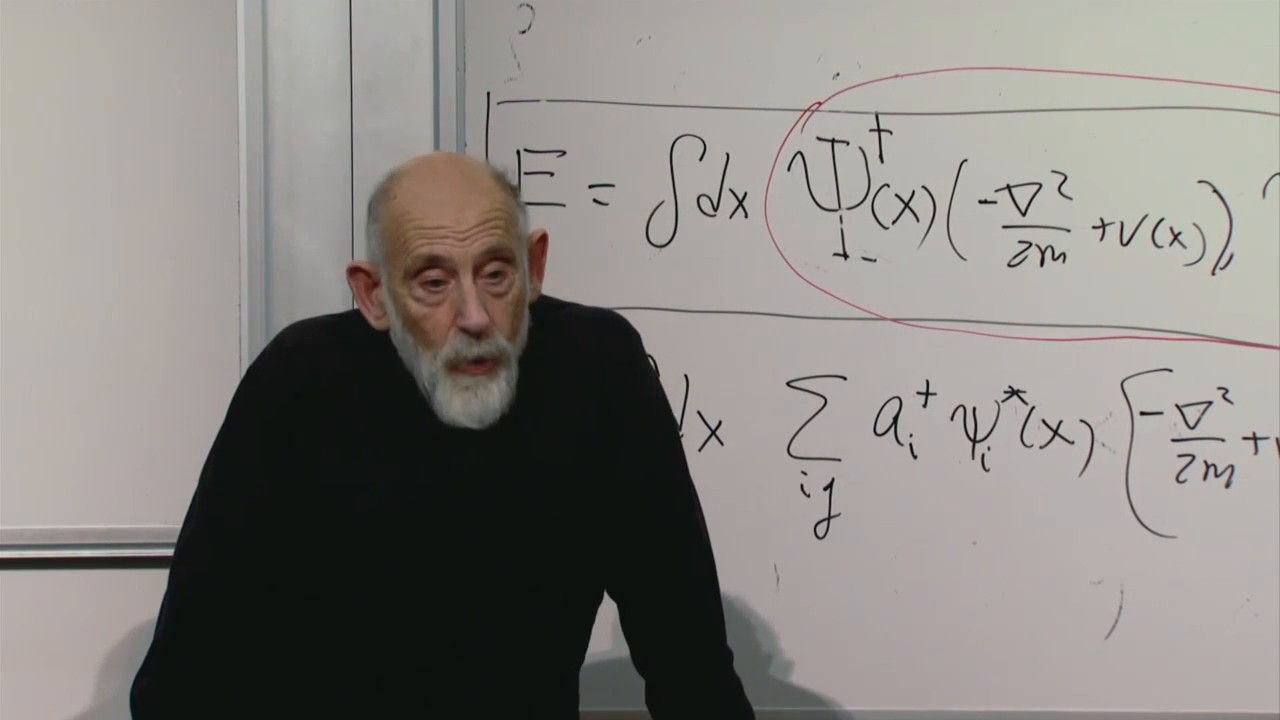
\includegraphics[width=0.94\linewidth]{lecture_07_frame_03.png}
\caption{El Hamiltoniano de campo destacado en la pizarra, con la demostración mediante la expansión en modos empezando debajo. Se conserva el fotograma de la clase como evidencia; las Ecuaciones~\eqref{eq:l07-field-hamiltonian}--\eqref{eq:l07-h-proof} restablecen el desarrollo algebraico completo.}
\lectureframe{01:05:34}
\end{figure}

En esta demostración no se ha conmutado ningún operador de creación a través de un operador de aniquilación. El orden \(a_i^\dagger a_j\) se mantiene de principio a fin. Los únicos objetos que se han desplazado libremente son las funciones de onda y sus autovalores, que son \(c\)-números.

\section{Por qué esto es un campo}

¿Por qué llamar campo a \(\Psi(x)\)? Porque es una cantidad con valores de operador definida en cada punto del espacio, y las combinaciones hermíticas o bilineales construidas a partir de ella son observables locales. La densidad \(n(x)\) y la expresión de energía local que aparece más adelante son dos ejemplos. La palabra no encierra ningún otro criterio matemático.

Este campo no es el campo electromagnético. Describe la especie no relativista que proporcionó los modos de una partícula y el Hamiltoniano \(p^2/(2m)+V\): por ejemplo, átomos lentos, neutrones, protones o electrones. Esas partículas son los cuantos de su campo correspondiente, en el mismo sentido estructural en que los fotones son los cuantos del campo electromagnético.

\begin{classroomqa}
\lecturetimestamp{01:02:45}
\audiencequestion{¿En qué momento, al pasar del sistema de muchas partículas a la fórmula anterior, aparece un campo?}
\lecturerresponse{Aparece en la Ecuación~\eqref{eq:l07-field-expansion}: \(\Psi(x)\) es un operador en cada punto espacial. Las derivaciones posteriores muestran que sus productos locales miden densidades de partículas y de energía. La dependencia de la posición, junto con el carácter de operador, es precisamente la estructura de campo que estamos construyendo.}
\end{classroomqa}

\section{Densidad local de energía}

La Ecuación~\eqref{eq:l07-field-hamiltonian} expresa la energía total como una integral sobre el espacio:
\begin{equation}
\begin{aligned}
H&=\int dx\,\mathcal H(x),\\
\mathcal H(x)
&=-\frac{1}{2m}\Psi^\dagger(x)\nabla^2\Psi(x)\\
&\quad+V(x)\Psi^\dagger(x)\Psi(x).
\end{aligned}
\label{eq:l07-hamiltonian-density}
\end{equation}
El integrando es una densidad local de energía natural para este Hamiltoniano. Su forma local no es única. Por ejemplo, una integración por partes sustituye el término cinético por
\begin{equation}
\mathcal H_{\rm kin}(x)
=\frac{1}{2m}\nabla\Psi^\dagger(x)\mathbin{\cdot}\nabla\Psi(x)
\label{eq:l07-kinetic-density}
\end{equation}
salvo por un término de contorno. Ambas expresiones dan el mismo Hamiltoniano total con las condiciones de contorno habituales. Esta es la pequeña ambigüedad mencionada en la clase.

\begin{classroomqa}
\lecturetimestamp{01:05:57}
\audiencequestion{¿Hay que integrar la densidad de energía sobre todo el espacio?}
\lecturerresponse{La integración sobre todo el espacio da la energía total. La integración sobre una región menor da la energía asignada a esa región, sujeta a la ambigüedad habitual al elegir una densidad local cuya integral sobre todo el espacio dé el mismo Hamiltoniano.}
\end{classroomqa}

\begin{classroomqa}
\lecturetimestamp{01:06:25}
\audiencequestion{¿En qué se diferencia la \(N_i\) mayúscula de la \(n_i\) minúscula en la fórmula de la energía?}
\lecturerresponse{\(N_i=a_i^\dagger a_i\) es un operador. El entero \(n_i\) es uno de sus autovalores en un estado de número de ocupación. Los operadores actúan sobre estados; sus autovalores son números ordinarios.}
\end{classroomqa}

\begin{classroomqa}
\lecturetimestamp{01:06:46}
\audiencequestion{¿Se puede escribir el propio Hamiltoniano de campo como un bra o un ket en la notación de Dirac?}
\lecturerresponse{No. Los bras y los kets representan vectores de estado y sus duales. El campo y el Hamiltoniano son operadores que actúan sobre esos estados. Un valor esperado como \(\langle\Phi|H|\Phi\rangle\) utiliza ambos tipos de objetos y no debe identificarlos.}
\end{classroomqa}

\section{Recuperar una partícula y acercarse a un campo clásico}

El formalismo ampliado contiene la mecánica cuántica ordinaria de una partícula. Restrinjamos el espacio de Fock a estados que satisfagan
\begin{equation}
N|\Phi\rangle=|\Phi\rangle.
\end{equation}
En ese sector, la construcción de campos reproduce todos los estados y todas las predicciones de una partícula. No hemos sustituido la teoría antigua; la hemos incorporado en un espacio que también puede describir cero, dos o un número arbitrario de partículas.

En el otro extremo, un modo ocupado por un número muy grande de bosones puede comportarse aproximadamente como una onda clásica. En estados coherentes o semiclásicos adecuados, el valor esperado
\begin{equation}
\Phi_{\rm cl}(x,t)=\langle\Psi(x,t)\rangle
\end{equation}
satisface la ecuación de aspecto clásico
\begin{equation}
i\partial_t\Phi_{\rm cl}(x,t)
=\left(-\frac{\nabla^2}{2m}+V(x)\right)\Phi_{\rm cl}(x,t)
\label{eq:l07-classical-schrodinger}
\end{equation}
para la teoría libre no relativista. La clase enuncia esta conexión, pero no la deriva. Es el puente entre una colección de cuantos y un campo ondulatorio: las ocupaciones grandes suprimen las fluctuaciones relativas y hacen que ciertos valores esperados se comporten clásicamente.

Por tanto, el formalismo es tanto un recurso para llevar la cuenta como una descripción física. Organiza todos los sectores de número de partículas, pero también recoge la interferencia, el entrelazamiento y la aparición de ondas clásicas a partir de partículas cuánticas.

\begin{classroomqa}
\lecturetimestamp{01:10:43}
\audiencequestion{¿Por qué se pueden manipular los operadores de creación y aniquilación dentro de la integral casi como si fueran números ordinarios?}
\lecturerresponse{Nunca se intercambiaron entre sí. Las funciones de modo ordinarias conmutan con ellos, y las derivadas actúan solo sobre esas funciones. Para pasar un operador de aniquilación a través de uno de creación habría que usar el conmutador, lo que podría añadir un término; la demostración no hace tal operación.}
\end{classroomqa}

\section{Un interludio sobre la notación de Dirac}

Parte de la confusión es histórica. Una función de onda de una partícula satisface una ecuación de ondas y se parece superficialmente a un campo clásico, aunque también es una amplitud de probabilidad. La teoría cuántica primitiva tuvo que separar esos papeles y luego explicar cómo los campos ondulatorios físicamente medibles, como el electromagnetismo, están formados por cuantos. El espacio de Fock y los campos con valores de operador resuelven el aparente conflicto.

La notación de Dirac hace que esta separación resulte excepcionalmente compacta. Un ket pertenece a un espacio vectorial, un bra a su dual, y al yuxtaponerlos se forma un producto interno. Entonces, la resolución
\begin{equation}
\sum_i|i\rangle\langle i|=\mathbf 1
\end{equation}
se vuelve casi autoexplicativa. La clase ilustra esto con una anécdota sobre la enseñanza de mecánica cuántica a matemáticos: el contenido matemático ya les resultaba familiar, pero la notación hacía tan transparentes las manipulaciones rutinarias que la estructura parecía nueva. La idea no es que a una disciplina le faltara el concepto. Es que una notación bien elegida puede hacer difícil confundir las operaciones permitidas.

Esta lección importa aquí. Ahora hay varios operadores distintos:
\begin{itemize}
\item \(h\) actúa sobre funciones de onda de una partícula como operador diferencial;
\item \(a_i\) y \(a_i^\dagger\) actúan sobre estados de número de ocupación en el espacio de Fock;
\item \(\Psi(x)\), \(\Psi^\dagger(x)\), \(N\) y \(H\) también actúan sobre el espacio de Fock.
\end{itemize}
La expansión de la Ecuación~\eqref{eq:l07-field-expansion} conecta los dos primeros contextos sin fundirlos.

\begin{classroomqa}
\lecturetimestamp{01:18:16}
\audiencequestion{¿Son los campos solo un formalismo para describir colecciones de partículas?}
\lecturerresponse{Son un formalismo, pero no uno vacío. Sus observables locales se pueden medir, y las partículas son partículas cuánticas con interferencia y entrelazamiento, no bolitas clásicas. Los operadores de campo codifican precisamente esas propiedades colectivas medibles.}
\end{classroomqa}

\section{Cautela relativista y una digresión sobre electromagnetismo}

La construcción hasta aquí es no relativista. El momento sigue siendo una buena etiqueta para las partículas en la física relativista, pero la posición de una partícula estrictamente localizada es mucho más delicada. Por consiguiente, una densidad local de número de fotones no suele ser un objeto tan limpio como \(n(x)\) en el caso no relativista. La densidad de energía sigue estando bien definida y es el observable local más seguro.

La clase ofrece una analogía electromagnética útil, explícitamente heurística. Combinemos los campos eléctrico y magnético en el vector complejo
\begin{equation}
\mathbf F=\mathbf E+i\mathbf B,
\qquad
\mathbf F^*=\mathbf E-i\mathbf B.
\label{eq:l07-riemann-silberstein}
\end{equation}
Entonces,
\begin{equation}
\mathbf F^*\mathbin{\cdot}\mathbf F
=\mathbf E^2+\mathbf B^2,
\label{eq:l07-em-density}
\end{equation}
que, en unidades convencionales, es proporcional a la densidad de energía electromagnética. Esto no es literalmente una densidad de probabilidad de fotones. Es mejor verlo como una variable de campo compacta cuyo módulo al cuadrado mide la densidad de energía o, informalmente, como una densidad de fotones ponderada por la energía de los fotones.

\begin{classroomqa}
\lecturetimestamp{01:19:10}
\audiencequestion{¿Se puede identificar la densidad de fotones con la intensidad del campo eléctrico?}
\lecturerresponse{Solo cualitativamente y con cautela. Para los fotones relativistas, el número local de partículas no es el concepto más adecuado. La afirmación sólida es que \(E^2+B^2\) es proporcional a la densidad de energía y que la combinación compleja \(\mathbf E+i\mathbf B\) expresa las ecuaciones de Maxwell en una forma parecida a la de Schrödinger.}
\end{classroomqa}

\begin{classroomqa}
\lecturetimestamp{01:20:09}
\audiencequestion{¿Por qué puede una partícula relativista tener un momento definido mientras que su posición es problemática?}
\lecturerresponse{El momento etiqueta de forma clara las representaciones relativistas de una partícula, mientras que la localización estricta entra en conflicto con la creación de partículas y con la descripción relativista mediante campos. Esta clase no desarrolla esa teoría; la advertencia señala el límite de la interpretación no relativista de la densidad que estamos usando.}
\end{classroomqa}

\section{Orden de operadores y constante del estado fundamental}

No se puede cambiar el orden de los operadores a la ligera. Para modos bosónicos,
\begin{equation}
a_i a_i^\dagger=a_i^\dagger a_i+1.
\end{equation}
Por consiguiente, sustituir el orden normal \(\Psi^\dagger h\Psi\) por el orden inverso \((h\Psi)\Psi^\dagger\), o por su versión integrada correspondiente, añade la contribución del conmutador. En una base de modos, es una suma aditiva de una unidad de energía cuántica por modo. Es la constante de energía del estado fundamental o de punto cero y, en un continuo, requiere regularización. La clase no aborda aquí ese asunto; solo advierte que los dos ordenamientos no son iguales.

\begin{classroomqa}
\lecturetimestamp{01:22:04}
\audiencequestion{¿Qué ocurre si se intercambian \(\Psi\) y \(\Psi^\dagger\) en el Hamiltoniano?}
\lecturerresponse{Hay que incluir su conmutador. Por tanto, invertir el orden añade una contribución independiente del estado al estado fundamental, en lugar de reproducir la misma expresión. El Hamiltoniano mostrado se mantiene en orden normal, \(\Psi^\dagger h\Psi\).}
\end{classroomqa}

\section{El momento como prueba final}

En los últimos minutos se repite una vez más la misma sustitución. Para una partícula,
\begin{equation}
\langle p\rangle_\psi
=\int dx\,\psi^*(x)\left(-i\partial_x\right)\psi(x).
\label{eq:l07-one-particle-momentum}
\end{equation}
Al reemplazar la función de onda por el campo, se obtiene el operador de momento total
\begin{equation}
P=\int dx\,\Psi^\dagger(x)\left(-i\partial_x\right)\Psi(x),
\label{eq:l07-field-momentum}
\end{equation}
o, en tres dimensiones,
\begin{equation}
\mathbf P=\int d^3x\,\Psi^\dagger(\mathbf x)
\left(-i\boldsymbol\nabla\right)\Psi(\mathbf x).
\end{equation}
Los campos transportan momento. Un láser suficientemente potente transfiere momento a una pared y ejerce una fuerza; en la descripción cuántica, ese momento del campo es la suma de los momentos de los fotones.

La ecuación~\eqref{eq:l07-field-momentum} es un operador, no un valor esperado. Dado un estado del espacio de Fock \(|\Phi\rangle\), se puede calcular
\begin{equation}
\langle P\rangle_\Phi=\langle\Phi|P|\Phi\rangle.
\end{equation}
Para formar un valor esperado se necesitan tanto un operador como un estado. Confundir el observable con su promedio borraría precisamente la distinción que la exposición se ha esforzado por establecer.

\begin{classroomqa}
\lecturetimestamp{01:26:02}
\audiencequestion{¿El momento del campo que se muestra es ya el momento promedio?}
\lecturerresponse{No. Es el operador hermítico que representa el observable. Para obtener un valor esperado, se proporciona un estado y se intercala el operador entre su bra y su ket; una medición aún puede fluctuar alrededor de ese promedio.}
\end{classroomqa}

Este es el punto natural para detenerse. Partiendo de las partículas, hemos construido campos locales de creación y aniquilación, los hemos usado para contar partículas y hemos reescrito la suma de las energías y los momentos de una partícula como operadores de campo. El siguiente paso no consiste en otro cambio de notación, sino en hacer que los operadores de campo representen procesos físicos: partículas que se desintegran, partículas que se dispersan y especies que se transforman unas en otras.

\chapter{Mezcla, oscilación, momentos dipolares eléctricos y operadores de campo}

Empezaremos apartándonos un poco del tema anunciado, con una pregunta sobre los neutrinos. Hay indicios de que los neutrinos tienen masa y de que sus tipos se mezclan. Si sus masas no son todas iguales, ¿cómo puede un tipo convertirse en otro sin violar la conservación de la energía?

La pregunta apunta a un patrón que aparece en toda la mecánica cuántica: los estados en los que se prepara o detecta un sistema no tienen por qué ser los que diagonalizan su hamiltoniano. Un estado de energía definida solo adquiere una fase. Un estado preparado como superposición de varias energías cambia porque sus componentes adquieren fases distintas. Esta distinción nos llevará de un pozo doble a la oscilación de neutrinos y la precesión del espín. Tras una digresión sobre el momento dipolar eléctrico del electrón, volveremos a la segunda cuantización y veremos la misma estructura de Fourier posición--momento en el nivel de los operadores.

\section{La mezcla como cuestión fundamental}

No es necesario que todos los neutrinos tengan la misma masa. Los estados propios de energía no se mezclan entre sí; cada uno evoluciona de manera independiente. Lo que llamamos \emph{tipo} o sabor de un neutrino está relacionado con la forma en que se produce y se detecta, y un estado de sabor puede ser una combinación lineal de estados propios de masa y energía. Esquemáticamente,
\begin{equation}
|\text{type}\rangle = \sum_n c_n |E_n\rangle .
\end{equation}
Así que lo correcto no es decir que los estados propios de energía se transforman unos en otros, sino que los estados llamados ``neutrino electrónico'' o ``neutrino muónico'' no tienen por qué ser, ellos mismos, estados propios de energía.

\begin{classroomqa}
\lecturetimestamp{00:00:09}
\audiencequestion{Si los neutrinos tienen masas distintas, ¿cómo pueden mezclarse y conservarse la energía?}
\lecturerresponse{Los estados propios de masa y energía no se transforman unos en otros. Los estados de sabor electrónico, muónico y tauónico son combinaciones lineales distintas de esos estados propios. Cada componente de masa evoluciona con su propia fase, y la interferencia modifica las probabilidades de sabor sin violar la conservación de la energía.}
\end{classroomqa}

Hay muchos ejemplos de esta estructura. El más visible comienza con una partícula en un pozo doble simétrico.

\section{Pozo doble simétrico y estados localizados aproximados}

Consideremos una partícula que se mueve en un potencial de doble pozo simétrico, con una barrera alta entre los dos mínimos. Si la barrera fuera infinitamente alta, los pozos izquierdo y derecho quedarían completamente desacoplados. Podríamos resolver el pozo de la izquierda como si el de la derecha no existiera, y viceversa. Las funciones de onda aproximadas del estado fundamental serían entonces un estado localizado a la izquierda \(\psi_L\) y otro localizado a la derecha \(\psi_R\), ambos con la misma energía \(E\).

En cada pozo aislado, el estado fundamental tiene las propiedades cualitativas habituales: es suave, no tiene nodos y se encuentra en la energía más baja posible compatible con el confinamiento. Pensemos en la alta barrera central como si fuera un muro de ladrillos. Considerarla infinita es solo una aproximación, pero nos proporciona un par útil de estados localizados como punto de partida.

\begin{figure}
\centering
\begin{adjustbox}{max width=\linewidth}
\begin{tikzpicture}[x=0.8cm,y=0.8cm]
\begin{scope}[shift={(-5.8,0)}]
\draw (-4,2.7) .. controls (-3.35,1.2) and (-2.55,-0.45) .. (-2.0,-0.72)
      .. controls (-1.35,-0.95) and (-0.7,0.65) .. (0,2.05)
      .. controls (0.7,0.65) and (1.35,-0.95) .. (2.0,-0.72)
      .. controls (2.55,-0.45) and (3.35,1.2) .. (4,2.7);
\draw[dashed] (-4,-0.10) -- (4,-0.10);
\node at (-3.55,-0.48) {$E$};
\draw[line width=0.9pt] (-4,-0.02) .. controls (-3.2,-0.02) and (-2.7,0.30) .. (-2.15,0.95)
      .. controls (-1.55,1.30) and (-1.15,0.35) .. (-0.55,-0.06)
      .. controls (0.15,-0.14) and (0.9,-0.15) .. (4,-0.15);
\node at (-2.15,1.35) {$\psi_L$};
\end{scope}
\begin{scope}[shift={(5.8,0)}]
\draw (-4,2.7) .. controls (-3.35,1.2) and (-2.55,-0.45) .. (-2.0,-0.72)
      .. controls (-1.35,-0.95) and (-0.7,0.65) .. (0,2.05)
      .. controls (0.7,0.65) and (1.35,-0.95) .. (2.0,-0.72)
      .. controls (2.55,-0.45) and (3.35,1.2) .. (4,2.7);
\draw[dashed] (-4,-0.10) -- (4,-0.10);
\node at (-3.55,-0.48) {$E$};
\draw[line width=0.9pt] (-4,-0.02) .. controls (-3.2,-0.01) and (-2.7,0.30) .. (-2.15,0.95)
      .. controls (-1.6,1.28) and (-1.1,0.25) .. (-0.30,-0.08)
      .. controls (0.35,-0.12) and (0.85,-0.12) .. (1.35,0.35)
      .. controls (1.9,0.88) and (2.35,1.15) .. (2.85,0.55)
      .. controls (3.2,0.05) and (3.55,-0.12) .. (4,-0.15);
\end{scope}
\end{tikzpicture}
\end{adjustbox}
\caption{Redibujo limpio de los primeros esquemas de la pizarra. A la izquierda está el estado de prueba unilateral \(\psi_L\), obtenido al suponer que la barrera es efectivamente infinita. A la derecha, la misma función de onda se prolonga simétricamente a través de la barrera, lo que ilustra la fuga pequeña pero no nula que acaba dando lugar al verdadero estado fundamental par.}
\end{figure}

Sin embargo, en mecánica cuántica la barrera no es realmente infinita. La función de onda en la región de la barrera no es exactamente cero; solo es muy pequeña. Toda la cuestión reside en esta fuga diminuta. Es lo que convierte la aproximación de izquierda y derecha en un verdadero problema de mezcla.

\section{Estados propios de paridad y desdoblamiento exponencial de niveles}

Ahora la imagen localizada queda interrumpida por un teorema: si el potencial es simétrico, las funciones propias exactas de la energía pueden elegirse simétricas o antisimétricas bajo reflexión.

\begin{theorem}
Si \(V(x)=V(-x)\) en una dimensión, las funciones propias del hamiltoniano pueden elegirse de modo que satisfagan una de estas dos condiciones:
\[
\psi(x)=\psi(-x)
\qquad \text{or} \qquad
\psi(x)=-\psi(-x).
\]
\end{theorem}

Ahora viene la corrección. Los estados unilaterales \(\psi_L\) y \(\psi_R\) no son ni simétricos ni antisimétricos, así que no pueden ser estados propios exactos del hamiltoniano completo. Solo son buenos estados aproximados cuando la barrera es alta. Los verdaderos estados propios son las combinaciones simétrica y antisimétrica,
\begin{align}
\psi_+ &= \frac{\psi_L+\psi_R}{\sqrt{2}},\\
\psi_- &= \frac{\psi_L-\psi_R}{\sqrt{2}}.
\end{align}
Con la notación que dejaremos en la pizarra, llamemos a sus energías
\begin{align}
H\psi_+ &= (E_1-\epsilon)\psi_+,\\
H\psi_- &= (E_1+\epsilon)\psi_-.
\end{align}
Por tanto, el desdoblamiento total es
\begin{equation}
\Delta E = (E_1+\epsilon)-(E_1-\epsilon)=2\epsilon .
\end{equation}

\begin{figure}[htbp]
\centering
\includegraphics[width=0.92\linewidth]{lecture_08_frame_02.png}
\caption{La función de onda prolongada simétricamente en el potencial de doble pozo. Su amplitud bajo la barrera es pequeña, pero no nula; de ahí se origina el desdoblamiento de niveles.}
\lectureframe{00:06:19}
\end{figure}

\begin{figure}
\centering
\begin{tikzpicture}[x=1cm,y=1cm]
\draw[->] (0,0) -- (0,3);
\node[left] at (0,2.8) {energy};
\draw (-0.35,1.60) -- (0.35,1.60);
\node[left] at (-0.45,1.60) {$\psi_L,\psi_R$};
\node at (1.7,1.60) {$\Longrightarrow$};
\draw (3.0,1.32) -- (3.75,1.32);
\draw (3.0,1.88) -- (3.75,1.88);
\draw[dashed] (2.8,1.60) -- (3.95,1.60);
\node[right] at (3.9,1.32) {$\psi_+,\ E_1-\epsilon$};
\node[right] at (3.9,1.88) {$\psi_-,\ E_1+\epsilon$};
\node[below] at (3.37,1.60) {$E_1$};
\end{tikzpicture}
\caption{El razonamiento de la pizarra sobre el desdoblamiento por efecto túnel. Los estados aproximados de izquierda y derecha son casi degenerados, pero los estados propios exactos, simétrico y antisimétrico, están separados por una pequeña cantidad \(2\epsilon\).}
\end{figure}

El orden de los niveles encierra el contenido físico. El estado simétrico tiene una energía ligeramente menor porque es más suave en la región de la barrera; permitir que la función de onda se filtre y continúe simétricamente reduce la energía en una cantidad diminuta. El estado antisimétrico tiene una energía ligeramente mayor porque el primer estado excitado en una dimensión tiene un nodo y, en este problema simétrico, ese nodo está en el punto medio. La curvatura adicional cuesta energía cinética.

El efecto es muy pequeño, exponencialmente pequeño en la anchura y la altura de la barrera. Aquí no necesitamos una fórmula explícita de WKB; lo importante es que el desdoblamiento es real, aunque diminuto. Recordemos también que el signo global de una función de onda no contiene información física. Sustituir \(\psi_-\) por \(-\psi_-\) no cambia el estado.

\section{Evolución temporal y oscilación entre izquierda y derecha}

Planteemos ahora la pregunta dinámica: ¿qué ocurre si colocamos una partícula en el pozo de la izquierda? Este es el paso decisivo, porque la oscilación es la manifestación temporal del mismo fenómeno de mezcla.

Las relaciones inversas son
\begin{align}
\psi_L &= \frac{\psi_+ + \psi_-}{\sqrt{2}},\\
\psi_R &= \frac{\psi_+ - \psi_-}{\sqrt{2}}.
\end{align}
Así, un estado inicialmente localizado a la izquierda es
\begin{equation}
\psi(0)=\psi_L=\frac{\psi_+ + \psi_-}{\sqrt{2}}.
\end{equation}
No es un estado propio de energía y, por tanto, debe evolucionar de manera no trivial.

Usamos la convención estándar de Schr\"odinger \(e^{-iEt}\). Una fase común no tiene efectos observables; solo la fase relativa entre los dos componentes de energía puede trasladar probabilidad de un pozo al otro.

Con esa convención,
\begin{equation}
\psi(t)=\frac{1}{\sqrt{2}}\left(e^{-i(E_1-\epsilon)t}\psi_+ + e^{-i(E_1+\epsilon)t}\psi_-\right).
\end{equation}
Esta es la versión depurada de la fórmula de la pizarra. Ahora saquemos factor común de la fase:
\begin{equation}
\psi(t)=\frac{e^{-iE_1 t}}{\sqrt{2}}\left(e^{i\epsilon t}\psi_+ + e^{-i\epsilon t}\psi_-\right).
\end{equation}
Una fase gira ahora en un sentido alrededor del círculo unidad y la otra en el sentido opuesto. El estado solo cambia porque estas dos fases se desfasan.

Para ver explícitamente la oscilación entre izquierda y derecha, sustituyamos las definiciones de \(\psi_\pm\):
\begin{align}
\psi(t)
&= \frac{e^{-iE_1 t}}{2}
\left[e^{i\epsilon t}(\psi_L+\psi_R)+e^{-i\epsilon t}(\psi_L-\psi_R)\right] \\
&= \frac{e^{-iE_1 t}}{2}
\left[(e^{i\epsilon t}+e^{-i\epsilon t})\psi_L+(e^{i\epsilon t}-e^{-i\epsilon t})\psi_R\right] \\
&= e^{-iE_1 t}\left[\psi_L\cos(\epsilon t)+i\,\psi_R\sin(\epsilon t)\right].
\end{align}
Esta es la derivación desarrollada clave del capítulo. En la aproximación de dos estados, con \(\psi_L\) y \(\psi_R\) ortonormales, las probabilidades son
\begin{equation}
P_L(t)=\cos^2(\epsilon t),
\qquad
P_R(t)=\sin^2(\epsilon t).
\end{equation}
Así que el sistema oscila. En los tiempos intermedios está realmente en una superposición; por ejemplo, cuando \(\epsilon t=\pi/4\), las probabilidades a ambos lados son iguales. Las fases evolucionan continuamente, y la localización cambia con ellas de manera continua.

La derivación en la pizarra aísla el primer instante en que cambia el signo relativo. Preguntamos cuándo se cumple
\begin{equation}
e^{-i\epsilon t}=-\,e^{i\epsilon t},
\end{equation}
que es el hito que se destaca en la pizarra. Al multiplicar ambos lados se obtiene
\begin{equation}
e^{2i\epsilon t}=-1.
\end{equation}
Para la primera vez que ocurre,
\begin{equation}
2\epsilon t=\pi,
\qquad\text{so}\qquad
t_{L\to R}=\frac{\pi}{2\epsilon}.
\end{equation}

\begin{figure}[htbp]
\centering
\includegraphics[width=0.94\linewidth]{lecture_08_frame_05.png}
\caption{Cálculo de la fase relativa en la pizarra. Los dos componentes de energía se vuelven opuestos cuando \(e^{2i\epsilon t}=-1\), lo que da el primer tiempo de transferencia \(2\epsilon t=\pi\). La derivación tipográfica emplea una sola convención de fase de Schr\"odinger.}
\lectureframe{00:17:52}
\end{figure}
En ese instante,
\begin{equation}
\psi(t_{L\to R}) \propto \frac{\psi_+-\psi_-}{\sqrt{2}}=\psi_R.
\end{equation}
La fase global es irrelevante. Lo que importa es que la partícula colocada inicialmente a la izquierda ha evolucionado hasta el estado localizado a la derecha. Tras otro intervalo igual, vuelve a oscilar hacia la izquierda. Mezcla y oscilación van juntas.

La ecuación no deja lugar a dudas: un valor pequeño de \(\epsilon\) implica oscilaciones lentas y un tiempo de transferencia largo. Ninguno de los dos estados localizados tiene energía definida, pero los dos componentes exactos de energía conservan la energía y evolucionan tal como deben.

\section{Analogías con neutrinos, amoníaco y espín}

El pozo doble nos proporciona un modelo para la pregunta original sobre los neutrinos. Un neutrino producido junto con un electrón se llama neutrino electrónico; uno producido junto con un muón se llama neutrino muónico. Esas etiquetas de sabor describen los canales de producción y detección. Los estados de masa definida y, por tanto, de energía definida para un momento fijo forman otra base.

En el modelo esquemático más sencillo de dos estados con mezcla máxima,
\begin{equation}
|\nu_e\rangle \sim \frac{|m_1\rangle+|m_2\rangle}{\sqrt{2}},
\qquad
|\nu_\mu\rangle \sim \frac{|m_1\rangle-|m_2\rangle}{\sqrt{2}},
\end{equation}
los estados propios de masa desempeñan el papel de \(\psi_+\) y \(\psi_-\), y los estados de sabor el de \(\psi_L\) y \(\psi_R\). La mezcla real de neutrinos utiliza una matriz de mezcla no trivial en lugar de estos coeficientes iguales, pero aquí ya se ve el mecanismo.

Un neutrino electrónico se produce en un proceso que involucra un electrón, igual que una partícula puede colocarse en el pozo de la izquierda. Durante un trayecto corto, sus dos componentes de masa acumulan fases casi iguales, por lo que una interacción todavía lo identifica como de sabor electrónico. A lo largo de una distancia grande, sus fases se separan. Entonces, una interacción posterior de corriente cargada puede producir un muón en vez de un electrón: el estado ha adquirido una componente de sabor muónico. Si se repite el experimento a distintas distancias o energías, se observa la oscilación.

No hay ningún conflicto con la conservación de la energía. Los estados propios de masa y energía hacen exactamente lo que deben hacer los estados propios. Lo que evoluciona es la superposición de sabores. En el límite relativista, la fase relativa observable está determinada por las diferencias de los cuadrados de las masas, esquemáticamente,
\begin{equation}
\Delta\phi_{ij}\simeq \frac{\Delta m_{ij}^{,2}L}{2E}.
\end{equation}
La oscilación muestra, por tanto, que no todas las masas de los neutrinos pueden ser idénticas: al menos dos estados propios de masa tienen masas distintas.

\begin{classroomqa}
\lecturetimestamp{00:24:06}
\audiencequestion{¿Qué determina el pequeño desdoblamiento \(\epsilon\) en el ejemplo del doble pozo?}
\lecturerresponse{Depende de la masa de la partícula y de la altura y anchura de la barrera. El efecto túnel es exponencialmente sensible a esos detalles, así que un cambio moderado en la barrera puede producir un gran cambio relativo en \(\epsilon\).}
\end{classroomqa}

\begin{classroomqa}
\lecturetimestamp{00:24:26}
\audiencequestion{¿Se ha observado realmente este fenómeno de oscilación?}
\lecturerresponse{Sí. Se observan desdoblamientos por efecto túnel en sistemas cuánticos ordinarios y oscilaciones de sabor en los neutrinos. Los mecanismos microscópicos son distintos, pero ambos realizan la misma evolución de fase en un sistema de dos estados.}
\end{classroomqa}

\begin{classroomqa}
\lecturetimestamp{00:24:34}
\audiencequestion{¿Qué relación hay entre la oscilación de neutrinos y la masa de los neutrinos?}
\lecturerresponse{Los estados propios que se propagan tienen masas distintas y, por tanto, acumulan fases distintas. Su interferencia modifica la composición de sabores. En un tratamiento relativista realista, lo que controla la oscilación son las diferencias de los cuadrados de las masas, no una masa de una partícula que varíe literalmente con el tiempo.}
\end{classroomqa}

\begin{classroomqa}
\lecturetimestamp{00:25:02}
\audiencequestion{¿La masa de los neutrinos es solo la teoría predominante o un hecho experimental?}
\lecturerresponse{La oscilación es un hecho experimental y requiere diferencias de masa distintas de cero. La escala absoluta de las masas es una magnitud distinta y más difícil de medir, pero los experimentos descartan la imagen mínima en la que todos los neutrinos carecen de masa.}
\end{classroomqa}

\subsection{Inversión del amoníaco: una barrera literal}

Una molécula de amoníaco, \(\mathrm{NH}_3\), tiene forma de pirámide trigonal: los tres átomos de hidrógeno forman un plano y el nitrógeno se encuentra a un lado de este. Existe una configuración equivalente con el nitrógeno al otro lado. Las dos configuraciones localizadas no son estados estacionarios exactos. El nitrógeno puede atravesar por efecto túnel el plano de hidrógeno, lo que produce estados propios de energía simétrico y antisimétrico y un pequeño desdoblamiento de inversión. Este es el origen físico de las mismas matemáticas en el máser de amoníaco.

\begin{classroomqa}
\lecturetimestamp{00:25:11}
\audiencequestion{En el amoníaco, ¿es la barrera la configuración en la que el nitrógeno atraviesa el plano de hidrógeno?}
\lecturerresponse{Sí. La energía molecular alcanza un mínimo en cualquiera de las dos configuraciones piramidales, mientras que la configuración plana tiene mayor energía. El efecto túnel a través de esta configuración acopla ambos lados.}
\end{classroomqa}

\begin{classroomqa}
\lecturetimestamp{00:27:10}
\audiencequestion{¿Cuál es la barrera física correspondiente entre los neutrinos electrónicos y muónicos?}
\lecturerresponse{No hay una barrera espacial literal. La analogía es algebraica: un acoplamiento no diagonal en el hamiltoniano de neutrinos mezcla la base de sabor. En el amoníaco, ese acoplamiento surge del efecto túnel; en los neutrinos, forma parte de la estructura de masas y mezcla.}
\end{classroomqa}

\subsection{Precesión del espín: mezcla sin efecto túnel}

Ya hemos encontrado el mismo álgebra en el espín. Tomemos los dos estados \(|\uparrow_z\rangle\) y \(|\downarrow_z\rangle\). Sin campo magnético son degenerados. Ahora apliquemos un campo magnético en la dirección \(x\). Los estados propios de energía ya no son los estados propios de \(z\), sino los estados polarizados en la dirección \(x\). Con los nombres provisionales izquierda--derecha de la pizarra,
\begin{align}
|L_x\rangle &= \frac{|\uparrow_z\rangle+|\downarrow_z\rangle}{\sqrt{2}},\\
|R_x\rangle &= \frac{|\uparrow_z\rangle-|\downarrow_z\rangle}{\sqrt{2}}.
\end{align}
Estos son los análogos directos de \(\psi_+\) y \(\psi_-\). El momento magnético alineado con el campo y el alineado en sentido opuesto tienen energías ligeramente distintas. Si esas energías son \(E\mp\epsilon\), un espín inicialmente hacia arriba evoluciona como sigue:
\begin{equation}
|\uparrow_z,t\rangle
= e^{-iEt}\left[\cos(\epsilon t)\,|\uparrow_z\rangle
+ i\sin(\epsilon t)\,|\downarrow_z\rangle\right].
\end{equation}
Esta es la misma fórmula que en el caso del doble pozo, solo que ahora la evolución continua corresponde a la precesión del espín alrededor del eje \(x\). Partiendo de \(+z\), el espín pasa por direcciones transversales, llega a \(-z\) tras medio período de precesión y vuelve después de otro medio período. Al medir \(S_z\) se obtiene todavía solo arriba o abajo; el estado de espín, que cambia continuamente, determina sus probabilidades. El mecanismo no requiere efecto túnel. Solo requiere que el hamiltoniano sea diagonal en una base distinta de la base de preparación.

\begin{classroomqa}
\lecturetimestamp{00:32:25}
\audiencequestion{¿Qué ocurre con el neutrino tauónico en este modelo?}
\lecturerresponse{También se mezcla. El problema real tiene tres estados de sabor y tres estados de masa, así que una matriz de mezcla de tres por tres reemplaza a la rotación de dos estados. El principio de interferencia de fases no cambia.}
\end{classroomqa}

\begin{classroomqa}
\lecturetimestamp{00:32:57}
\audiencequestion{Justo después de aplicar el campo transversal, ¿el espín sigue apuntando hacia arriba? ¿Puede orientarse hacia nosotros o en sentido opuesto?}
\lecturerresponse{Al cabo de un tiempo muy corto, sigue apuntando hacia arriba con una probabilidad casi segura, aunque existe una pequeña probabilidad de que apunte hacia abajo. El estado precesa continuamente alrededor del eje del campo y pasa por las direcciones transversales \(\pm y\), mientras permanece perpendicular al campo dirigido según \(x\) si inicialmente era perpendicular. Una medición a lo largo de cualquier eje elegido sigue dando uno de sus valores propios discretos.}
\end{classroomqa}

\begin{classroomqa}
\lecturetimestamp{00:34:30}
\audiencequestion{¿Se elige un campo débil para que el espín nunca apunte en la dirección del campo?}
\lecturerresponse{No. La geometría se debe a la precesión alrededor del eje del campo, no a que el campo sea débil. Un campo débil simplemente hace pequeña la separación de energía y la frecuencia de precesión, lo que produce una oscilación lenta análoga al ejemplo de los neutrinos.}
\end{classroomqa}

La intensidad de la mezcla de neutrinos y sus pequeñas masas son parámetros cuyo origen más profundo no explica el Modelo Estándar mínimo tal como se formuló originalmente. Por tanto, la masa de los neutrinos apunta más allá de ese modelo mínimo, aunque la escala observada es muy pequeña y podría reflejar física a una escala de energía muy remota.

\begin{classroomqa}
\lecturetimestamp{00:36:27}
\audiencequestion{¿Es la oscilación la razón por la que sabemos que los neutrinos tienen masa?}
\lecturerresponse{Es la prueba directa decisiva de que los componentes que se propagan tienen masas distintas. Si todos los componentes pertinentes fueran exactamente sin masa y degenerados, no acumularían ninguna fase relativa dependiente de la masa y no habría una oscilación de sabor en el vacío de este tipo.}
\end{classroomqa}

\begin{classroomqa}
\lecturetimestamp{00:37:57}
\audiencequestion{A mitad de un período, ¿debería un neutrino comportarse la mitad de las veces como de sabor electrónico y la otra mitad como de sabor muónico?}
\lecturerresponse{En el modelo ideal simétrico de dos estados, las probabilidades son iguales a un cuarto del período completo de probabilidad, mientras que la conversión completa ocurre en el primer máximo. Las oscilaciones reales de tres sabores tienen ángulos de mezcla desiguales, varias frecuencias, restricciones de espín y helicidad, y efectos de la materia, así que una conversión simétrica completa no es lo habitual.}
\end{classroomqa}

\begin{classroomqa}
\lecturetimestamp{00:38:36}
\audiencequestion{Si los componentes de masa son distintos, ¿debe cambiar la velocidad de un neutrino solar para conservar el momento?}
\lecturerresponse{Un estado de sabor es una superposición coherente de componentes de masas fijas; su masa no es una magnitud clásica que oscile con el tiempo. En la descripción habitual de momento igual, los componentes tienen energías y velocidades de grupo ligeramente distintas; en una descripción de energía igual, tienen momentos ligeramente distintos. Ambas convenciones dan la misma fase de oscilación observable si se tratan de manera coherente.}
\end{classroomqa}

Esta evolución de fase resolvió el antiguo déficit de neutrinos solares. Los primeros detectores eran sensibles principalmente a los neutrinos electrónicos, así que los neutrinos que salían del Sol como de sabor electrónico podían llegar en parte como muónicos o tauónicos y dejar de ser detectados en ese canal. El cálculo solar detallado incluye la mezcla de tres sabores y efectos de la materia, pero la lección conceptual ya está en el doble pozo: la preparación y la propagación utilizan bases distintas.

\section{Digresión: momento dipolar eléctrico, simetría y la afirmación de que el electrón es una ``esfera''}

Como ya estamos hablando de fenomenología de partículas, hagamos una pausa en las matemáticas formales. Un artículo divulgativo describió un nuevo límite para el momento dipolar eléctrico del electrón diciendo que se había demostrado que el electrón era una esfera. Ese eslogan confunde tres preguntas distintas: qué mide un momento dipolar eléctrico, qué significa la simetría rotacional para un estado cuántico y qué limitó realmente el experimento.

\subsection{¿Qué se midió?}

Lo que se midió —o, mejor dicho, se acotó— fue el momento dipolar eléctrico del electrón. Para cargas separadas \(\pm q\), el momento dipolar es
\begin{equation}
\mathbf d = q\,\boldsymbol{\ell},
\end{equation}
donde \(\boldsymbol{\ell}\) es el vector de separación. Un momento dipolar distinto de cero significa que la distribución de carga está desplazada respecto de cierto centro.

Para el electrón, sin embargo, la pregunta pertinente no es simplemente si la carga está descentrada en alguna dirección arbitraria. El electrón tiene espín y, por tanto, un eje. También tiene un momento magnético. La pregunta físicamente significativa es si existe una correlación entre el desplazamiento de la carga y ese eje:
\begin{equation}
\mathbf d_e \parallel \boldsymbol{\mu}_e
\qquad \text{or equivalently} \qquad
\mathbf d_e \parallel \mathbf S .
\end{equation}
A eso nos referimos con el momento dipolar eléctrico del electrón. Conceptualmente, nos preguntamos si, al colocar un electrón polarizado en espín en un campo eléctrico, se separan en energía las dos orientaciones del espín:
\begin{equation}
H_{\mathrm{EDM}}=-\mathbf d_e\cdot \mathbf E,
\qquad
\mathbf d_e=d_e\frac{\mathbf S}{|\mathbf S|}.
\end{equation}
El experimento real de sobremesa es mucho más sutil que un electrón desnudo entre las placas de un condensador, pero esta es la idea de simetría y cambio de energía que aprovecha.

\subsection{Por qué la ausencia de EDM no significa que sea una esfera}

La primera corrección es elemental. Un cuerpo puede no tener momento dipolar y aun así no ser esférico. Un elipsoide centrado tiene tanta carga a un lado como al otro y, por tanto, no tiene dipolo; sin embargo, puede tener un momento cuadrupolar. Una distribución aún más complicada puede carecer tanto de dipolo como de cuadrupolo y conservar un multipolo de orden superior. Medir un coeficiente multipolar no determina una forma completa.

La mecánica cuántica hace más delicada la palabra ``forma''. Imaginemos una molécula de dos átomos, parecida a una mancuerna, con una longitud de enlace aproximadamente fija. Ignoremos las vibraciones radiales y consideremos solo las rotaciones. Los estados rotacionales se etiquetan por el momento angular. Si la molécula es bosónica, el estado rotacional más bajo tiene \(J=0\). Como el momento angular genera las rotaciones,
\begin{equation}
\begin{gathered}
J=0 \quad\Longrightarrow\\
\text{rotationally invariant ground state.}
\end{gathered}
\end{equation}
El estado cuántico es invariante bajo rotaciones, aunque toda imagen con orientación definida parece una mancuerna. Puede describirse como una superposición coherente de todas las orientaciones. Llamar ``esférico'' al estado resulta útil para algunas mediciones y engañoso para otras.

Tomemos una instantánea. Una instantánea es una medición de la orientación, y una medición de orientación suficientemente precisa deja al sistema en un estado localizado en ángulo. Ese estado no puede tener también un momento angular definido. Esta es la versión rotacional del principio de incertidumbre posición--momento: localizar el ángulo necesariamente introduce una dispersión de momentos angulares y, por tanto, excitación rotacional.

Para un rotor rígido,
\begin{equation}
E_J=\frac{J(J+1)}{2I},
\end{equation}
por lo que la energía necesaria para resolver la estructura está determinada por el momento de inercia \(I\). Una mancuerna de gimnasio tiene un \(I\) enorme y niveles rotacionales extraordinariamente próximos; la luz ordinaria puede perturbarla con facilidad lo suficiente para revelar una orientación. En una molécula, la separación entre niveles es mayor. En un hadrón compacto, lo es aún más. Si la sonda no tiene energía suficiente para excitar la primera estructura rotacional resoluble, las mediciones repetidas solo ven el estado fundamental promediado sobre las rotaciones.

Un mesón puede imaginarse, de manera aproximada, como un sistema de dos cuerpos formado por un quark--antiquark. Sus primeras excitaciones orbitales cuestan cientos de millones de electronvoltios o más, muy por encima de la energía de un fotón óptico. Por tanto, una sonda de baja energía no puede tomar una instantánea de la orientación subyacente. ``Que sea una esfera o no'' depende en parte del estado preparado y en parte de la resolución del aparato.

El electrón precisa aún más la cuestión. Es una partícula de espín \(\tfrac12\), no un escalar rotacional. Un estado polarizado en espín tiene un eje y un momento magnético. La imagen habitual de una carga que circula alrededor de ese eje es solo una heurística---una partícula de Dirac puntual no es literalmente una pequeña esfera que gira---, pero nos recuerda correctamente que el momento magnético se invierte con el espín. La pregunta sobre el EDM es si el desplazamiento de carga eléctrica está correlacionado con ese mismo eje. Una respuesta nula no convierte al electrón en una esfera clásica.

\begin{classroomqa}
\lecturetimestamp{00:57:30}
\audiencequestion{¿El desplazamiento de parte de la carga del electrón violaría la cuantización de la carga?}
\lecturerresponse{No. La cuantización de la carga fija la carga total. El momento dipolar se refiere al primer momento espacial de esa distribución de carga o, de manera equivalente, a un acoplamiento permitido de una partícula puntual con el campo eléctrico; no requiere un cambio fraccionario de la carga total.}
\end{classroomqa}

\begin{classroomqa}
\lecturetimestamp{00:58:00}
\audiencequestion{¿Están prohibidos los momentos dipolares eléctricos por la teoría cuántica de campos?}
\lecturerresponse{La teoría cuántica de campos en sí no los prohíbe. Quedan prohibidos cuando ciertas simetrías discretas son exactas. Si se violan esas simetrías, se permite un operador EDM, aunque su coeficiente pueda ser extremadamente pequeño.}
\end{classroomqa}

\subsection{Paridad e inversión temporal}

El contenido real de la discusión sobre el EDM es la simetría. Bajo paridad, un momento dipolar eléctrico se transforma como un vector polar ordinario, mientras que un momento magnético se transforma como un vector axial:
\begin{align}
P:\qquad &\mathbf d_e \to -\mathbf d_e,
&\boldsymbol{\mu}_e \to \boldsymbol{\mu}_e .
\end{align}
Bajo inversión temporal, la corriente circulante que define el momento magnético se invierte, pero un desplazamiento electrostático no:
\begin{align}
T:\qquad &\mathbf d_e \to \mathbf d_e,
&\boldsymbol{\mu}_e \to -\boldsymbol{\mu}_e .
\end{align}
Por tanto, un EDM distinto de cero alineado con el eje de espín del electrón está prohibido si la simetría de paridad es exacta y también si la simetría de inversión temporal es exacta:
\begin{equation}
(P\ \text{exact}) \Rightarrow \mathbf d_e=0,
\qquad
(T\ \text{exact}) \Rightarrow \mathbf d_e=0.
\end{equation}

Conviene explicitar la geometría. Un momento magnético se produce mediante una corriente en forma de lazo. La reflexión especular invierte los vectores polares ordinarios, pero deja inalterado el vector axial normal a ese lazo. El desplazamiento de carga a lo largo del eje sí se invierte. Así, un electrón con \(\mathbf d_e\) paralelo a \(\boldsymbol\mu_e\) se transformaría por reflexión especular en uno con la misma orientación magnética, pero con la relación entre los momentos eléctrico y magnético invertida. Si la paridad fuera exacta y solo hubiera una especie de electrón, las dos descripciones tendrían que representar la misma partícula; solo \(d_e=0\) es compatible.

La inversión temporal lleva a la misma conclusión de otra manera. Al reproducir la película al revés, la corriente se invierte y, por tanto, también \(\boldsymbol\mu_e\), pero el desplazamiento estático de carga no cambia. Un estado con momentos paralelos pasa a ser uno con momentos antiparalelos. La simetría exacta bajo inversión temporal exigiría de nuevo \(d_e=0\).

\begin{figure}[htbp]
\centering
\begin{tikzpicture}[>=Stealth,scale=0.95]
  \node[font=\bfseries] at (1.0,2.25) {original};
  \draw[->,very thick,blue!70!black] (0.65,0) -- (0.65,1.65);
  \draw[->,very thick,red!75!black] (1.35,0) -- (1.35,1.65);
  \node[blue!70!black,below] at (0.65,0) {$\boldsymbol\mu$};
  \node[red!75!black,below] at (1.35,0) {$\mathbf d$};

  \node[font=\bfseries] at (4.5,2.25) {parity};
  \draw[->,very thick,blue!70!black] (4.15,0) -- (4.15,1.65);
  \draw[->,very thick,red!75!black] (4.85,1.65) -- (4.85,0);
  \node[blue!70!black,below] at (4.15,0) {$\boldsymbol\mu$};
  \node[red!75!black,below] at (4.85,0) {$-\mathbf d$};

  \node[font=\bfseries] at (8.0,2.25) {time reversal};
  \draw[->,very thick,blue!70!black] (7.65,1.65) -- (7.65,0);
  \draw[->,very thick,red!75!black] (8.35,0) -- (8.35,1.65);
  \node[blue!70!black,below] at (7.65,0) {$-\boldsymbol\mu$};
  \node[red!75!black,below] at (8.35,0) {$\mathbf d$};
\end{tikzpicture}
\caption{La prueba de simetría reconstruida a partir del argumento en la pizarra. La paridad invierte el dipolo eléctrico, pero no el momento magnético axial; la inversión temporal invierte el momento magnético, pero no el desplazamiento eléctrico estático. Si cualquiera de estas simetrías fuera exacta, prohibiría un EDM permanente paralelo al espín.}
\end{figure}

\begin{figure}[htbp]
\centering
\includegraphics[width=0.94\linewidth]{lecture_08_frame_06.png}
\caption{Los esquemas emparejados del eje magnético y el desplazamiento de carga durante el argumento sobre la inversión temporal. El diagrama compacto en TikZ de arriba aísla el contenido de las transformaciones de la pizarra original, parcialmente borrada.}
\lectureframe{01:06:10}
\end{figure}

\begin{classroomqa}
\lecturetimestamp{01:06:38}
\audiencequestion{Bajo inversión temporal, ¿se invierten tanto las corrientes como las cargas?}
\lecturerresponse{Las corrientes se invierten porque las velocidades se invierten; la carga eléctrica en sí no. La conjugación de carga \(C\), y no la inversión temporal \(T\), invierte el signo de la carga.}
\end{classroomqa}

\begin{classroomqa}
\lecturetimestamp{01:07:01}
\audiencequestion{¿El carácter antiunitario de la inversión temporal significa que la mecánica cuántica no relativista no es invariante bajo inversión temporal?}
\lecturerresponse{No. La antiunitariedad es precisamente la forma de representar la inversión temporal de manera coherente en mecánica cuántica: conjuga complejamente las amplitudes e invierte los momentos y los espines. Que un Hamiltoniano particular sea invariante es una cuestión distinta.}
\end{classroomqa}

\begin{classroomqa}
\lecturetimestamp{01:07:19}
\audiencequestion{¿Para hablar de un EDM es necesario que el electrón tenga un volumen finito, en vez de ser puntual?}
\lecturerresponse{No. Un Hamiltoniano efectivo para una partícula puntual puede contener \(-d_e\,\widehat{\mathbf S}\!\cdot\!\mathbf E\). El experimento pregunta si orientaciones opuestas del espín adquieren energías distintas en un campo eléctrico; no es necesario resolver una nube de carga extensa literal.}
\end{classroomqa}

La paridad no es una simetría de las interacciones débiles; se viola al máximo en sus acoplamientos quirales. La inversión temporal tampoco es exacta, pero la violación conocida en el Modelo Estándar contribuye al EDM del electrón solo a un nivel extraordinariamente pequeño. Se puede calcular una contribución no nula del Modelo Estándar, pero queda muy por debajo de la sensibilidad de la que hablamos aquí. Por tanto, un resultado nulo es compatible con el Modelo Estándar, aunque restringe extensiones---la supersimetría y otras interacciones nuevas, por ejemplo---que pueden generar una violación de la inversión temporal mucho mayor.

La idea experimental básica es sencilla. Un campo magnético revela un dipolo magnético al separar las orientaciones del espín. Un campo eléctrico revelaría un EDM mediante un desplazamiento adicional de la energía correlacionado con el espín. Los experimentos de precisión reales emplean átomos o moléculas, largos tiempos de precesión coherente, inversiones de los campos aplicados y un control cuidadoso de los efectos sistemáticos, en vez de un electrón aislado en un dispositivo ingenuo.

\begin{classroomqa}
\lecturetimestamp{01:11:02}
\audiencequestion{¿La búsqueda del EDM fue un experimento de colisiones de alta energía o un experimento con objetos materiales?}
\lecturerresponse{Fue un experimento de precisión de sobremesa, con electrones ligados en un entorno atómico o molecular controlado, junto con campos eléctricos y magnéticos. Su energía es baja, pero su sensibilidad a desplazamientos minúsculos que violan simetrías permite sondear indirectamente nueva física de alta energía.}
\end{classroomqa}

\begin{classroomqa}
\lecturetimestamp{01:12:21}
\audiencequestion{¿El resultado nulo restringe cuáles modificaciones del Modelo Estándar siguen siendo viables?}
\lecturerresponse{Sí, en principio: cada modelo predice un coeficiente y, por tanto, ocupa cierta región de parámetros. La exclusión numérica detallada requiere un cálculo especializado, pero la lógica general es firme---cuanto mayor es la precisión con que concuerdan los resultados con el Modelo Estándar, menos margen queda para alternativas que predigan un EDM grande.}
\end{classroomqa}

\begin{classroomqa}
\lecturetimestamp{01:13:09}
\audiencequestion{¿Se requiere la simetría bajo inversión temporal para conservar la información cuántica?}
\lecturerresponse{No. La evolución temporal unitaria conserva la información incluso cuando un Hamiltoniano no es invariante bajo \(T\). Una partícula en un campo magnético fijo es un ejemplo conocido: el campo selecciona una orientación en las películas invertidas temporalmente, a menos que también se invierta el campo, pero la evolución cuántica sigue siendo unitaria. Bajo las hipótesis habituales de la teoría cuántica de campos local e invariante de Lorentz, la transformación combinada \(CPT\) es una simetría, pero eso no es lo que garantiza la unitariedad.}
\end{classroomqa}

El descanso puede terminar ahora. La medición nula indica que no se ha detectado ningún EDM del electrón con la sensibilidad indicada. No afirma que el electrón sea una esfera ni refuta el Modelo Estándar; hace más difícil sostener algunas desviaciones propuestas respecto de ese modelo.

\section{Regreso a la segunda cuantización: transformadas de Fourier, modos de momento y localidad}

Estábamos estudiando la segunda cuantización. Empecemos de nuevo con calma, a partir de un hecho conocido sobre las funciones de onda ordinarias de una partícula, y luego extendámoslo a los operadores. La conexión con las transformadas de Fourier es exacta y sencilla.

\subsection{Del espacio de posiciones al espacio de momentos}

La letra minúscula \(\psi\), no la mayúscula \(\Psi\), representa la función de onda de una sola partícula. En el espacio de posiciones,
\begin{equation}
P(x)=|\psi(x)|^2
\end{equation}
es la densidad de probabilidad de encontrar la partícula en la posición \(x\). La función de onda en el espacio de momentos es su transformada de Fourier,
\begin{equation}
\tilde{\psi}(p)=\int dx\,\psi(x)\,\frac{e^{-ipx}}{\sqrt{2\pi}},
\end{equation}
y la relación inversa es
\begin{equation}
\psi(x)=\int dp\,\tilde{\psi}(p)\,\frac{e^{ipx}}{\sqrt{2\pi}}.
\end{equation}
Entonces,
\begin{equation}
P(p)=|\tilde{\psi}(p)|^2
\end{equation}
es la densidad de probabilidad del momento \(p\).

Usamos \(\hbar=1\). Las dos transformadas son inversas: conocer cualquiera de las dos funciones de onda determina la otra, mientras que sus módulos al cuadrado responden a preguntas de medición distintas.

Para una partícula libre,
\begin{equation}
H=\frac{p^2}{2m},
\end{equation}
por lo que los estados propios del momento también son estados propios de la energía, y sus funciones de onda en el espacio de posiciones son ondas planas,
\begin{equation}
\psi_p(x)\propto e^{ipx}.
\end{equation}
Este es el punto de partida para la versión en segunda cuantización.

\begin{figure}[htbp]
\centering
\includegraphics[width=0.94\linewidth]{lecture_08_frame_07.png}
\caption{Par de Fourier entre posición--momento para una función de onda de una partícula. Es esencial distinguir \(\psi\) del operador de campo, que se introduce a continuación.}
\lectureframe{01:20:00}
\end{figure}

\subsection{Operadores de campo en los espacios de posiciones y de momentos}

Volvamos ahora al operador de campo. En la pizarra, sus partes de aniquilación y creación se escriben como \(\Psi_-(x)\) y \(\Psi_+(x)\). Manteniendo por un momento esa notación,
\begin{align}
\Psi_-(x) &= \sum_i a_i\,\psi_i(x),\\
\Psi_+(x) &= \sum_i a_i^\dagger\,\psi_i^*(x).
\end{align}
Aquí, \(\psi_i(x)\) es la función de onda ordinaria de una partícula para el modo \(i\), mientras que \(a_i\) y \(a_i^\dagger\) aniquilan y crean partículas en ese modo. A partir de aquí conviene cambiar la notación a
\[
\Psi(x)\equiv \Psi_-(x),
\qquad
\Psi^\dagger(x)\equiv \Psi_+(x).
\]

Para una partícula libre, la etiqueta discreta del modo \(i\) se sustituye por la etiqueta continua del momento \(p\). Usando las ondas planas \(e^{ipx}\), se obtienen las fórmulas reconstruidas habituales
\begin{align}
\Psi(x) &= \int \frac{dp}{\sqrt{2\pi}}\,a(p)\,e^{ipx},\\
\Psi^\dagger(x) &= \int \frac{dp}{\sqrt{2\pi}}\,a^\dagger(p)\,e^{-ipx}.
\end{align}
Estas son las fórmulas análogas a la transformada de Fourier ordinaria para los operadores de campo. Se pueden invertir exactamente como antes:
\begin{align}
a(p) &= \int \frac{dx}{\sqrt{2\pi}}\,\Psi(x)\,e^{-ipx},\\
a^\dagger(p) &= \int \frac{dx}{\sqrt{2\pi}}\,\Psi^\dagger(x)\,e^{ipx}.
\end{align}
Los factores de \(1/\sqrt{2\pi}\) son una convención elegida para que las transformadas directa e inversa tengan la misma normalización.

El contenido conceptual es sencillo. \(\Psi^\dagger(x)\) crea una partícula en la posición \(x\), mientras que \(a^\dagger(p)\) crea una partícula con momento \(p\). Los operadores de creación en los espacios de posiciones y de momentos son conjugados de Fourier entre sí, igual que \(\psi(x)\) y \(\tilde{\psi}(p)\) lo son en la mecánica cuántica ordinaria.

Si no hay ninguna partícula con momento \(p\), \(a(p)\) aniquila el estado. Si hay partículas con ese momento, elimina una con el coeficiente habitual del número de ocupación. Del mismo modo, \(\Psi(x)\) elimina una partícula en \(x\), entendido en el sentido de distribuciones o tras integrar el campo para formar un paquete de ondas. Cada especie de partícula requiere su propio operador de campo; un único campo no puede crear todas las clases de partículas.

\subsection{Conmutadores bosónicos e independencia de las mediciones en regiones separadas}

El siguiente resultado se deduce directamente de las definiciones. Para los bosones,
\begin{equation}
[a_i,a_j^\dagger]=\delta_{ij},
\qquad
[a_i,a_j]=0,
\qquad
[a_i^\dagger,a_j^\dagger]=0.
\end{equation}
La versión continua es
\begin{equation}
[a(p),a^\dagger(p')]=\delta(p-p').
\end{equation}
Calculemos ahora el conmutador de los campos a tiempos iguales a partir de la expansión discreta:
\begin{align}
[\Psi(x),\Psi^\dagger(y)]
&= \sum_{i,j}\psi_i(x)\psi_j^*(y)\,[a_i,a_j^\dagger] \\
&= \sum_i \psi_i(x)\psi_i^*(y) \\
&= \delta(x-y),
\end{align}
donde el último paso usa la completitud de la base de una partícula. Asimismo,
\begin{equation}
[\Psi(x),\Psi(y)]=0,
\qquad
[\Psi^\dagger(x),\Psi^\dagger(y)]=0.
\end{equation}

\begin{figure}[htbp]
\centering
\includegraphics[width=0.94\linewidth]{lecture_08_frame_08.png}
\caption{El conmutador de los modos y su correspondiente en el espacio de posiciones, tal como aparecen en la pizarra. La completitud convierte \(\delta_{ij}\) en la distribución delta espacial \(\delta(x-y)\).}
\lectureframe{01:31:00}
\end{figure}

Lo importante no es solo que \(\Psi\) no sea hermítico. Definamos las cuadraturas hermíticas
\begin{equation}
Q(x)=\frac{\Psi(x)+\Psi^\dagger(x)}{\sqrt{2}},
\qquad
P(x)=\frac{\Psi(x)-\Psi^\dagger(x)}{i\sqrt{2}}.
\end{equation}
Su conmutador en un mismo punto hereda la distribución delta. Así, las dos cuadraturas locales son conjugadas en el mismo sentido en que lo son la posición y el momento. Intentar precisar una aumenta la incertidumbre de la otra.

\begin{classroomqa}
\lecturetimestamp{01:32:03}
\audiencequestion{¿Qué significa la función delta cuando \(x=y\)? ¿Es grande el conmutador en todas partes?}
\lecturerresponse{La delta es una distribución, no una función ordinaria con un valor finito en cada punto. Se anula para argumentos separados y solo da un resultado finito al integrarla contra una función de prueba. Al integrar los campos sobre una región finita del detector, la singularidad formal en un mismo punto se convierte en el conmutador canónico finito habitual de dos modos.}
\end{classroomqa}

Sin embargo, para \(x\neq y\), el conmutador a tiempos iguales se anula. Las operaciones localizadas en dos regiones disjuntas pueden realizarse de forma independiente: medir el campo aquí no da una sacudida cuántica al campo allí. Este es el antecedente no relativista, a tiempos iguales, de la microcausalidad relativista. En una teoría relativista, los observables locales físicos conmutan cuando están separados espacialmente, pues ninguna señal luminosa puede conectar los dos eventos.

El contraste con los observables que no conmutan es conocido. Como \([x,p]=i\), una medición precisa de la posición perturba el momento, y un estado con momento preciso se dispersa en posición. Como las distintas componentes del espín no conmutan, preparar una de ellas con precisión hace que otra sea incierta. Un conmutador no nulo entre observables locales separados significaría, de manera análoga, que una operación en una región perturba la otra, en contradicción con la independencia causal requerida.

\begin{classroomqa}
\lecturetimestamp{01:37:51}
\audiencequestion{¿Los experimentos EPR y de entrelazamiento demuestran que una medición aquí afecta a una medición distante?}
\lecturerresponse{Demuestran que hay correlaciones, no una influencia causal controlable. Los resultados entrelazados violan la factorización clásica, pero no se pueden cambiar las estadísticas locales del detector distante eligiendo o realizando aquí una medición. La conmutación de observables separados espacialmente es la formulación en términos de operadores de esa independencia que impide la señalización.}
\end{classroomqa}

La próxima vez cambiará el álgebra. Los operadores de creación y aniquilación de fermiones satisfacen relaciones de anticonmutación. Tomado al pie de la letra, los campos fermiónicos en puntos separados no conmutan, de modo que los propios campos no pueden interpretarse directamente como observables bosónicos medibles. Los observables fermiónicos físicos son combinaciones pares---densidades, corrientes, tensores de energía-momento---y esos observables locales recuperan la conmutatividad requerida para separaciones espaciales. Ese es el punto de partida para la versión fermiónica de la segunda cuantización.

\chapter{Campos cuánticos locales y ecuación de Dirac unidimensional}

Ya hemos conocido los campos cuánticos a través de sus cuantos, sus operadores de creación y aniquilación, y el Hamiltoniano más sencillo para partículas no relativistas. Ahora pondremos en funcionamiento ese formalismo. Primero veremos, en lugar de limitarnos a afirmarlo, cómo un Hamiltoniano espacialmente local conserva el momento. Después dejaremos que los productos de campos describan dispersión y desintegración, y observaremos cómo la acción repetida del Hamiltoniano genera los primeros elementos de la teoría de perturbaciones diagramática. Solo entonces abordaremos el problema de los fermiones que habíamos anunciado. La forma más sencilla de empezar no es todavía con un campo fermiónico, sino con la ecuación de Dirac unidimensional.

\section{De nuevo, el Hamiltoniano de campo}

Escribamos el Hamiltoniano para una especie de partículas no relativistas como
\begin{equation}
H_0=\int dx\,
\psi^\dagger(x)
\left[-\frac{\partial_x^2}{2m}+V(x)\right]
\psi(x).
\label{eq:l9-nonrel-hamiltonian}
\end{equation}
La notación parece unidimensional, pero nada en el argumento inicial depende de esa restricción: en tres dimensiones, \(x\) puede representar el vector \(\mathbf{x}\), \(dx\) puede representar \(d^3x\) y \(-\partial_x^2\) puede representar \(-\nabla^2\).

El operador \(\psi^\dagger(x)\) crea una partícula en \(x\), mientras que \(\psi(x)\) aniquila una en ese punto. Su producto normalmente ordenado
\begin{equation}
n(x)=\psi^\dagger(x)\psi(x)
\end{equation}
es la densidad local de partículas. Por tanto, el término de potencial es
\begin{equation}
H_V=\int dx\,V(x)n(x).
\end{equation}
exactamente lo que escribiríamos para un gas clásico: contar las partículas cerca de \(x\), asignar a cada una la energía potencial \(V(x)\) y sumarlas en todo el espacio. En esta etapa, las partículas no interactúan entre sí. Pueden responder a un potencial externo aplicado, pero, por lo demás, el Hamiltoniano es una suma de energías independientes de una partícula.

Conviene simplificar y luego volver sobre nuestros pasos. Supongamos que el potencial es constante, \(V(x)=V_0\). Un potencial constante no ejerce fuerza, pero su significado como operador es transparente:
\begin{equation}
\begin{aligned}
H_V&=V_0\int dx\,\psi^\dagger(x)\psi(x)=V_0N,\\
N&=\int dx\,n(x).
\end{aligned}
\end{equation}
Asigna a cada partícula la misma energía aditiva. Para conservar la energía en reposo en una descripción no relativista, elijamos \(V_0=mc^2\). El término cuenta entonces una energía en reposo por partícula. Conservamos esta constante, por lo demás anodina, porque preserva la invariancia traslacional y hace visible la operación de contar partículas.

\section{El Hamiltoniano como regla de actualización}

¿Qué significa decir que se conserva el momento? Debemos formular la respuesta en términos de lo que hace el Hamiltoniano. Para no usar \(\psi\) a la vez para un operador de campo, una función de onda de una partícula y un estado de muchos cuerpos, llamemos \(\lvert\Phi(t)\rangle\) al estado de muchos cuerpos. Durante un intervalo breve \(\epsilon\),
\begin{equation}
\lvert\Phi(t+\epsilon)\rangle
=\left(1-i\epsilon H+O(\epsilon^2)\right)
\lvert\Phi(t)\rangle,
\label{eq:l9-short-update}
\end{equation}
donde \(\hbar=1\). El primer término es el estado sin cambios; la primera corrección la genera \(H\). Iterar esta actualización da la ecuación de Schr\"odinger.

La conservación del momento adquiere ahora un significado concreto. Si el estado inicial tiene un momento total definido \(P\), entonces \(H\lvert\Phi\rangle\) debe tener ese mismo momento total. Otras propiedades pueden cambiar y las partículas individuales pueden intercambiar momento, pero el Hamiltoniano no puede llevar el estado a un sector con un \(P\) total distinto. Podemos comprobarlo directamente reescribiendo el Hamiltoniano en la base de momentos.

\section{La integral espacial como delta de Dirac en el momento}

Elijamos la convención de Fourier
\begin{align}
\psi(x)&=\int\frac{dp}{\sqrt{2\pi}}\,a(p)e^{ipx},\\
\psi^\dagger(x)&=\int\frac{dq}{\sqrt{2\pi}}\,a^\dagger(q)e^{-iqx}.
\label{eq:l9-field-fourier}
\end{align}
El operador \(a(p)\) aniquila una partícula de momento \(p\).
El operador \(a^\dagger(q)\) crea una partícula de momento \(q\). Es esencial usar letras distintas: los dos momentos se integran de forma independiente hasta que la integral espacial los relaciona.

Empecemos por el término de número:
\begin{align}
N
&=\int dx\,\psi^\dagger(x)\psi(x)\\
&=\int\frac{dp\,dq}{2\pi}\,
a^\dagger(q)a(p)
\int dx\,e^{i(p-q)x}.
\end{align}
La integral restante es
\begin{equation}
\int dx\,e^{i(p-q)x}=2\pi\delta(p-q).
\end{equation}
Para \(p\ne q\), la fase oscila y sus contribuciones positivas y negativas se cancelan. Para \(p=q\), no oscila en absoluto. La distribución delta de Dirac es el objeto preciso que reúne ambos hechos. Por consiguiente,
\begin{align}
N
&=\int dp\,dq\,a^\dagger(q)a(p)\delta(p-q)\\
&=\int dp\,a^\dagger(p)a(p).
\label{eq:l9-number-momentum}
\end{align}
El operador elimina una partícula de momento \(p\) y vuelve a crear una con exactamente el mismo momento. El elemento decisivo fue la integral sobre \(x\): produjo la delta que impone la igualdad entre el momento entrante y el saliente.

\begin{classroomqa}
\lecturetimestamp{00:17:02}
\audiencequestion{¿Qué ocurre con el infinito que aparece cuando \(p=q\)?}
\lecturerresponse{Una delta no se utiliza evaluando su altura. Es una distribución definida mediante integración: \(\int dk\,\delta(k)f(k)=f(0)\). La expresión ``infinitamente alta e infinitamente estrecha'' solo nos recuerda que su peso integrado es uno. Aquí nos indica que fijemos \(p-q=0\), y no queda ningún resultado infinito.}
\end{classroomqa}

El mismo mecanismo funciona para un monomio local mucho más general. Supongamos que un término contiene varios campos de aniquilación y varios campos de creación, quizá de especies distintas, pero todos evaluados en un mismo punto e integrados sobre ese punto:
\begin{equation}
\int dx\,
\prod_{r=1}^{n} \psi_{i_r}^\dagger(x)
\prod_{s=1}^{m} \psi_{j_s}(x).
\end{equation}
Sean \(p_s\) los momentos de las partículas aniquiladas y \(q_r\) los de las creadas. El desarrollo de Fourier produce
\begin{equation}
\int dx\,
e^{i(\sum_s p_s-\sum_r q_r)x}
=2\pi\,
\delta\!\left(\sum_s p_s-\sum_r q_r\right).
\label{eq:l9-total-momentum-delta}
\end{equation}
El resultado no empareja \(p_1\) con \(q_1\), \(p_2\) con \(q_2\), y así sucesivamente. Solo impone que
\begin{equation}
\sum_{\mathrm{annihilated}}p
=
\sum_{\mathrm{created}}q.
\end{equation}
Esa es precisamente la regla que debe cumplir una interacción: los momentos individuales pueden cambiar, pero el momento total se conserva. La afirmación más profunda es la invariancia traslacional. Una densidad local integrada con el mismo peso en todos los puntos no tiene un origen preferido, y su transformada de Fourier lleva la delta correspondiente que conserva el momento.

\begin{classroomqa}
\lecturetimestamp{00:23:04}
\audiencequestion{¿El término propuesto del Hamiltoniano es realmente un producto de todos esos operadores de campo? ¿Por qué escribiríamos un producto así?}
\lecturerresponse{Sí. El producto especifica qué partículas se eliminan y cuáles se crean en un mismo punto. Su motivación física provendrá de los procesos de dispersión o desintegración observados; primero establecemos el argumento sobre el momento para poder identificar esas interacciones de inmediato.}
\end{classroomqa}

\section{La energía cinética en el espacio de momentos y de posiciones}

Apliquemos ahora el mismo formalismo al término con derivadas. La derivada actúa sobre la onda plana:
\begin{equation}
-\partial_x^2 e^{ipx}=p^2e^{ipx}.
\end{equation}
Por tanto,
\begin{align}
H_{\mathrm{kin}}
&=\int dx\,\psi^\dagger(x)
\left(-\frac{\partial_x^2}{2m}\right)\psi(x)\\
&=\int dp\,\frac{p^2}{2m}\,a^\dagger(p)a(p).
\label{eq:l9-kinetic-momentum}
\end{align}
De nuevo, la integral espacial impone que el momento entrante y el saliente sean iguales. El nuevo factor \(p^2/2m\) simplemente pondera el número de partículas de cada modo de momento por la energía cinética de ese modo.

\begin{classroomqa}
\lecturetimestamp{00:24:46}
\audiencequestion{¿Al derivar dos veces la onda plana no debería aparecer un signo menos?}
\lecturerresponse{Sí, \(\partial_x^2e^{ipx}=-p^2e^{ipx}\). El Hamiltoniano ya contiene el signo menos compensatorio, de modo que \(-\partial_x^2\) tiene el autovalor positivo \(p^2\).}
\end{classroomqa}

\begin{classroomqa}
\lecturetimestamp{00:27:20}
\audiencequestion{¿Solo se conserva la energía cinética cuando el potencial es constante?}
\lecturerresponse{Sí. Si no hay un potencial dependiente de la posición, no hay fuerza y la energía cinética se conserva por separado. En un potencial externo no constante, la energía cinética y la potencial pueden intercambiarse, mientras que el Hamiltoniano total se conserva si no depende explícitamente del tiempo.}
\end{classroomqa}

\begin{classroomqa}
\lecturetimestamp{00:27:42}
\audiencequestion{¿Qué función cumple \(\psi^\dagger\psi\) en el Hamiltoniano cinético en el espacio de momentos?}
\lecturerresponse{Es el operador de número. El producto de modos \(a^\dagger(p)a(p)\) cuenta las partículas de momento \(p\), y el factor \(p^2/2m\) asigna a cada una la energía cinética correspondiente.}
\end{classroomqa}

Hay otra forma de ver que la energía es positiva. Una integración por partes y el descarte del término de frontera dan
\begin{align}
\int dx\,\psi^\dagger(-\partial_x^2)\psi
&=\int dx\,(\partial_x\psi^\dagger)(\partial_x\psi).
\label{eq:l9-positive-kinetic}
\end{align}
Para campos que se anulan de manera adecuada en el infinito, o con condiciones de contorno periódicas, la contribución de frontera es cero. El resultado tiene la forma de un cuadrado de módulo y es no negativo. También muestra un patrón común en la teoría de campos: la energía contiene cuadrados de derivadas espaciales de los campos.

\section{Una interacción local de contacto}

Démosles ahora a los productos de campos una función física. Consideremos dos especies, a las que llamaremos electrón y protón solo para que la imagen resulte familiar. Por ahora son deliberadamente ficticias: ambas se describen mediante operadores bosónicos y se omite su verdadera interacción de Coulomb. Su Hamiltoniano libre es
\begin{equation}
H_0=\int dx\left[
\psi_e^\dagger\left(-\frac{\partial_x^2}{2m_e}\right)\psi_e
+
\psi_p^\dagger\left(-\frac{\partial_x^2}{2m_p}\right)\psi_p
\right].
\end{equation}
Añadamos la interacción modelo
\begin{equation}
H_{\mathrm{contact}}
=g\int dx\,
\psi_e^\dagger(x)\psi_p^\dagger(x)
\psi_e(x)\psi_p(x).
\label{eq:l9-contact}
\end{equation}
Leámosla de derecha a izquierda. Busca un electrón y un protón en el mismo punto \(x\), los aniquila y vuelve a crear ambos en ese punto. Si las dos partículas no están juntas, este término local da cero. Si sus líneas de universo se encuentran, puede cambiar sus momentos individuales y conservar el momento total. Así, actúa como un potencial de dispersión idealizado de alcance nulo.

\begin{figure}[htbp]
\centering
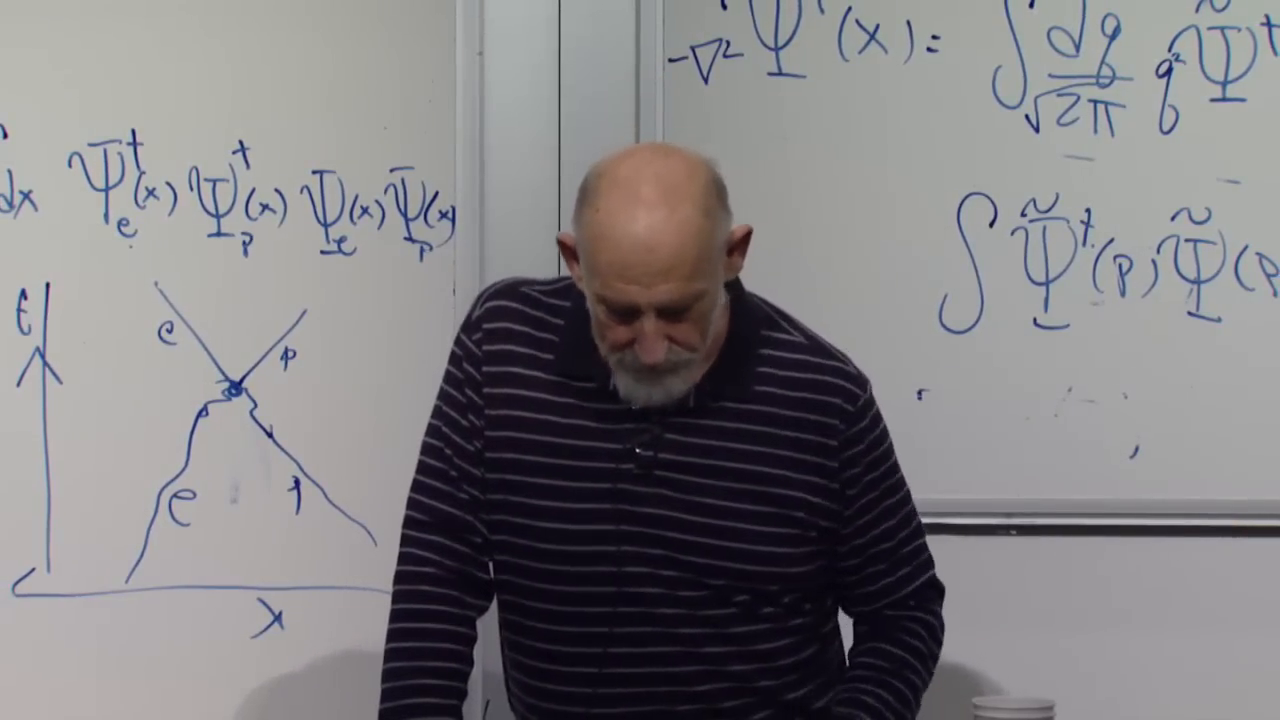
\includegraphics[width=0.94\linewidth]{lecture_09_frame_02.png}
\caption{La interacción de contacto en la pizarra. Los cuatro operadores de campo locales aparecen sobre el esquema espaciotemporal; el punto de encuentro es el único lugar donde actúa la interacción idealizada.}
\lectureframe{00:35:36}
\end{figure}

\begin{figure}[htbp]
\centering
\begin{tikzpicture}[x=1.2cm,y=1.0cm,>=Latex]
\draw[->] (-3.0,0) -- (3.0,0) node[right] {$x$};
\draw[->] (0,-0.2) -- (0,4.2) node[above] {$t$};
\coordinate (v) at (0,2.0);
\fill (v) circle (1.8pt);
\draw[thick,->] (-2.2,0.4) -- (v);
\draw[thick,->] (2.0,0.4) -- (v);
\draw[thick,->] (v) -- (-1.6,3.7);
\draw[thick,->] (v) -- (2.2,3.7);
\node[left] at (-1.65,0.7) {$e$};
\node[right] at (1.55,0.7) {$p$};
\node[left] at (-1.15,3.3) {$e$};
\node[right] at (1.65,3.3) {$p$};
\node[right] at (0.12,2.05) {$g$};
\end{tikzpicture}
\caption{Reconstrucción limpia de la imagen de dispersión local. El vértice es una abreviatura del operador de la ecuación~\eqref{eq:l9-contact}, no una ley clásica de colisión.}
\end{figure}

Los electrones y protones reales interactúan a distancia mediante el potencial de Coulomb. El modelo de contacto es solo un primer paso, válido para distancias cortas: si los experimentos mostraran que dos especies se dispersan únicamente cuando se solapan, incluiríamos en el Hamiltoniano un término del tipo de la ecuación~\eqref{eq:l9-contact}.

\begin{classroomqa}
\lecturetimestamp{00:35:40}
\audiencequestion{¿Por qué forma parte del Hamiltoniano este operador de dispersión si la energía no cambia?}
\lecturerresponse{El Hamiltoniano es tanto el operador de energía como el generador de cambios en el estado. La energía potencial entre las dos partículas produce dispersión durante la evolución temporal. Que se conserve la energía total no significa que el estado o los momentos individuales de las partículas permanezcan inalterados.}
\end{classroomqa}

Esto da una regla práctica. Primero, averigüemos mediante experimentos qué procesos locales pueden experimentar las partículas. Después, codifiquemos esos procesos en el operador que actualiza el estado. Los productos de campos no son álgebra decorativa: sus factores con daga y sin daga especifican qué especies aparecen y desaparecen.

\section{Desintegración, proceso inverso y hermiticidad}

Supongamos que en una cámara de burbujas se observa una traza de la especie \(A\) que termina en un punto del que emergen trazas de \(B\) y \(C\). El proceso local es
\begin{equation}
A\longrightarrow B+C.
\end{equation}
El operador que lo realiza es
\begin{equation}
V=g\int dx\,
\psi_B^\dagger(x)\psi_C^\dagger(x)\psi_A(x).
\label{eq:l9-decay-half}
\end{equation}
El campo de aniquilación elimina \(A\); los dos campos de creación producen \(B\) y \(C\) en el mismo punto. Integrar con el mismo peso sobre cada \(x\) expresa la invariancia traslacional espacial y proporciona inmediatamente
\begin{equation}
p_A=p_B+p_C.
\end{equation}

Un Hamiltoniano debe ser hermítico. Esto es lo que hace que \(e^{-itH}\) sea unitario y preserve la probabilidad total. La ecuación~\eqref{eq:l9-decay-half} no es hermítica por sí sola, así que debemos añadir su adjunto:
\begin{equation}
H_{\mathrm{int}}
=\int dx\left[
g\,\psi_B^\dagger\psi_C^\dagger\psi_A
+g^*\,\psi_A^\dagger\psi_C\psi_B
\right](x).
\label{eq:l9-hermitian-vertex}
\end{equation}
Para un acoplamiento real \(g\), los dos coeficientes son iguales. La conjugación hermítica invierte el orden de los operadores, además de intercambiar los campos con daga y sin daga. En este modelo bosónico de juguete, los campos de especies distintas conmutan, por lo que esa inversión no introduce complicaciones adicionales.

El segundo término realiza el proceso inverso,
\begin{equation}
B+C\longrightarrow A.
\end{equation}
Así, un Hamiltoniano cerrado y unitario que permite la desintegración también contiene la amplitud de recombinación. Esto no garantiza que ambas direcciones ocurran para cualquier conjunto de momentos externos: las leyes de conservación de la energía y otras pueden impedir que una de ellas sea cinemáticamente accesible. Significa que tanto el operador como su adjunto forman parte de la dinámica.

\begin{classroomqa}
\lecturetimestamp{00:42:48}
\audiencequestion{¿Puede haber una excepción a la regla de que también se permite el proceso inverso?}
\lecturerresponse{No en el marco de un Hamiltoniano hermítico de un sistema cerrado: se requiere la interacción adjunta. Una reacción inversa concreta aún puede verse impedida por la cinemática o por otro número cuántico conservado, pero el elemento de matriz conjugado está presente.}
\end{classroomqa}

El número \(g\) es la constante de acoplamiento. Si \(g\) es pequeño, las partículas que se encuentran interactúan débilmente; si es grande, la amplitud de transición es mayor. Por lo general, los acoplamientos son parámetros medidos experimentalmente, aunque las simetrías pueden relacionar varios acoplamientos que a primera vista parecen distintos.

La misma estructura permite describir reacciones más elaboradas. En la desintegración beta,
\begin{equation}
n\longrightarrow p+e^-+\bar\nu_e,
\end{equation}
un término local esquemático contiene cuatro campos: uno aniquila el neutrón y tres crean el protón, el electrón y el antineutrino electrónico, junto con el proceso conjugado hermítico. Esto basta para ver cómo un pequeño conjunto de monomios de operadores empieza a definir una teoría cuántica de campos.

\section{Por qué importa el cuadrado del Hamiltoniano}

La fórmula para tiempos cortos \eqref{eq:l9-short-update} solo conservaba los términos de primer orden en \(\epsilon\). El desarrollo completo es
\begin{equation}
e^{-i\epsilon H}
=1-i\epsilon H-\frac{\epsilon^2}{2}H^2
+\frac{i\epsilon^3}{3!}H^3+\cdots.
\label{eq:l9-exponential}
\end{equation}
A segundo orden, el Hamiltoniano actúa dos veces. Este es el origen algebraico de las primeras representaciones de procesos compuestos.

Para el vértice \(A\leftrightarrow B+C\), una acción puede combinar \(B+C\) para formar \(A\), y una segunda puede descomponer ese \(A\) de nuevo en \(B+C\):
\begin{equation}
B+C\longrightarrow A\longrightarrow B+C.
\label{eq:l9-bc-scattering}
\end{equation}
La contribución neta es una amplitud de dispersión \(B+C\to B+C\). El estado intermedio \(A\) no es un suceso observado adicional; indica el estado sobre el que se suma entre dos acciones de la interacción.

\begin{classroomqa}
\lecturetimestamp{00:49:54}
\audiencequestion{¿El campo de \(C\) de la expresión escrita de segundo orden debería llevar una daga?}
\lecturerresponse{Sí, el orden de los operadores debe corresponder a la secuencia indicada. El primer vértice aniquila \(B\) y \(C\), y crea \(A\); el segundo aniquila \(A\) y vuelve a crear \(B\) y \(C\). Escribir correctamente las dagas correspondientes restablece esa interpretación.}
\end{classroomqa}

\begin{figure}[htbp]
\centering
\includegraphics[width=0.94\linewidth]{lecture_09_frame_05.png}
\caption{Las dos orientaciones del vértice elemental \(A\leftrightarrow B+C\) en la pizarra. Colocarlas una junto a otra es la representación visual abreviada del proceso de segundo orden de la ecuación~\eqref{eq:l9-bc-scattering}.}
\lectureframe{00:48:56}
\end{figure}

Añadamos ahora un \(B\) espectador. Una acción permite que \(A\) emita \(C\) y se convierta en \(B\); una acción posterior permite que ese \(C\) se combine con el \(B\) original para formar \(A\). Las partículas externas vuelven a ser \(A+B\), pero sus momentos pueden cambiar. Describimos esto como dispersión de \(A\) y \(B\) mediante el intercambio de \(C\).

\begin{figure}[htbp]
\centering
\includegraphics[width=0.94\linewidth]{lecture_09_frame_06.png}
\caption{La construcción de intercambio en la pizarra. El diagrama de la derecha une dos vértices elementales mediante una línea interna de \(C\), mientras las partículas externas \(A\) y \(B\) se dispersan.}
\lectureframe{00:51:22}
\end{figure}

\begin{figure}[htbp]
\centering
\begin{tikzpicture}[x=1.1cm,y=1cm,>=Latex]
\draw[->] (-3.7,-0.2) -- (-3.7,4.2) node[above] {$t$};
\coordinate (v1) at (-0.9,1.25);
\coordinate (v2) at (0.9,2.95);
\fill (v1) circle (1.7pt);
\fill (v2) circle (1.7pt);
\draw[thick,->] (-2.6,0.2) -- (v1) node[midway,below left] {$A$};
\draw[thick,->] (2.6,0.2) -- (v2) node[midway,below right] {$B$};
\draw[thick,->] (v1) -- (-2.4,4.0) node[midway,left] {$B$};
\draw[thick,->] (v2) -- (2.5,4.0) node[midway,right] {$A$};
\draw[thick,->,dashed] (v1) -- (v2) node[midway,above left] {$C$};
\node[below] at (0,-0.05) {$A+B\rightarrow A+B$};
\end{tikzpicture}
\caption{Reconstrucción limpia del intercambio de \(C\). Cada punto aporta un factor de \(g\), por lo que este término de segundo orden es proporcional a \(g^2\).}
\end{figure}

Cada punto de interacción local se denomina vértice. Cada vértice aporta un factor de su acoplamiento, así que una contribución con dos vértices lleva \(g^2\), una con tres vértices lleva \(g^3\), y así sucesivamente. Por tanto, un solo término del Hamiltoniano correlaciona una gran familia de reacciones. Esta economía es una de las razones por las que la teoría cuántica de campos es tan potente: un pequeño número de interacciones locales organiza una enorme cantidad de datos de dispersión.

\begin{classroomqa}
\lecturetimestamp{00:53:14}
\audiencequestion{¿Cómo se llama el proceso \(A\to B+C\to A\)?}
\lecturerresponse{Es una contribución de autoenergía. Un \(A\) medido no es simplemente el estado de base desnudo de una partícula; el estado interactuante también tiene una amplitud para componentes cercanas \(B+C\). La dispersión desde ese estado puede revelar su estructura vestida.}
\end{classroomqa}

La electrodinámica cuántica ofrece el ejemplo conocido. Un vértice local electrón--fotón puede aniquilar un electrón, volver a crear un electrón y crear un fotón. A segundo orden, el electrón puede emitir y reabsorber un fotón. Es tentador narrarlo como una pequeña película, pero su significado preciso es el de un término en el desarrollo perturbativo. El electrón físico es un estado vestido con componentes que contienen fotones.

La estimación didáctica de que esta componente es ``aproximadamente un uno por ciento'' transmite la escala que fija la constante de estructura fina, \(\alpha_{\mathrm{em}}\simeq 1/137\). La probabilidad precisa de una componente del espacio de Fock con fotones depende de la resolución energética y de cómo se defina el estado interactuante; no es una propiedad universal de un electrón aislado que valga un uno por ciento. La afirmación robusta es que la interacción modifica la estructura medible del electrón.

\section{Qué representa un diagrama y qué no}

Los diagramas son una abreviatura de cálculo para las potencias del Hamiltoniano de interacción. No son historias clásicas fiables en las que una partícula realiza definitivamente un suceso y luego otro. Mirar en el interior para decidir qué alternativa intermedia ``ocurrió realmente'' cambia el experimento y destruye la suma coherente, igual que en la interferencia cuántica ordinaria.

\begin{classroomqa}
\lecturetimestamp{00:56:52}
\audiencequestion{¿Se conservan tanto la energía como el momento en el primer vértice?}
\lecturerresponse{En la construcción hamiltoniana a tiempo igual que hemos realizado aquí, la integral espacial produce inmediatamente una delta de momento. En esa inserción aislada aún no se ha realizado ninguna integral temporal que produzca una delta de energía. La amplitud de dispersión completa, invariante bajo traslaciones temporales, conserva la energía total, mientras que las líneas intermedias no tienen por qué satisfacer la relación de capa de masa de las partículas observadas. En el lenguaje de los diagramas covariantes, el cuadrimomento se conserva en cada vértice, pero las partículas internas pueden estar fuera de la capa de masa.}
\end{classroomqa}

La aparente falta de energía en una imagen ingenua del vértice es otra advertencia de que no se debe descartar la energía de interacción. El Hamiltoniano total es más que la suma de las energías de las partículas libres. Si surge alguna confusión, volvamos a la ecuación~\eqref{eq:l9-exponential}: la imagen representa un término del desarrollo de la evolución temporal unitaria. El formalismo completo de los diagramas de Feynman proporciona ordenamiento temporal sistemático, propagadores, integrales y factores de simetría, pero la física básica empieza aquí.

Una pregunta más extensa lleva a interpretar el diagrama de forma demasiado literal al comparar el fotón emitido con el campo eléctrico que rodea a un electrón que se mueve lentamente.

\begin{classroomqa}
\lecturetimestamp{00:58:26}
\audiencequestion{¿El campo eléctrico del electrón a distancia lo producen literalmente fotones radiados? ¿Cómo encaja esto con la interferencia y el efecto Aharon--Bohm?}
\lecturerresponse{Un campo estático o de inducción no es un flujo de fotones reales radiados. La electrodinámica cuántica describe tanto la radiación como el vestido electromagnético del electrón mediante el mismo campo, pero los estados cuánticos y la cinemática correspondientes son distintos. Para un electrón ultrarrelativista, algunos componentes del campo pueden comportarse útilmente como un flujo de fotones casi reales; para un electrón lento, una trayectoria literal de fotones es un modelo incorrecto. La interferencia de doble rendija y el efecto Aharon--Bohm también son fenómenos de campo no clásicos, pero no convierten este diagrama de autoenergía en una película mecánica.}
\end{classroomqa}

\begin{classroomqa}
\lecturetimestamp{01:01:28}
\audiencequestion{¿Por qué falla exactamente un modelo clásico del diagrama?}
\lecturerresponse{Porque el cálculo suma coherentemente las amplitudes de todas las alternativas intermedias permitidas. La experiencia hace intuitivas estas imágenes, pero su contenido literal nunca va más allá del desarrollo de operadores que las define. Son una forma compacta de calcular \(H^2,H^3,\ldots\), no un registro de sucesos intermedios observados.}
\end{classroomqa}

\begin{classroomqa}
\lecturetimestamp{01:03:04}
\audiencequestion{¿Puede surgir la interacción de Coulomb ordinaria como límite clásico del intercambio de fotones?}
\lecturerresponse{Sí. Al evaluar la amplitud pertinente mediada por fotones y tomar el límite estático no relativista se obtiene el potencial de Coulomb. La derivación es más técnica que el esquema de operadores que presentamos aquí, y aun así no debe interpretarse como si un fotón saltara literalmente entre dos partículas clásicas.}
\end{classroomqa}

\begin{classroomqa}
\lecturetimestamp{01:03:44}
\audiencequestion{¿Se calculan las constantes de acoplamiento a partir de los productos de campos?}
\lecturerresponse{Por lo general, sus valores numéricos se introducen a partir de datos experimentales. Las simetrías pueden restringirlos o relacionar acoplamientos que de otro modo serían independientes. Cuando una relación así predice las intensidades relativas de reacciones distintas y el experimento la confirma, esa concordancia aporta información especialmente valiosa.}
\end{classroomqa}

\begin{classroomqa}
\lecturetimestamp{01:04:48}
\audiencequestion{¿Qué papel tiene una simetría accidental frente a una simetría gauge?}
\lecturerresponse{La simetría gauge restringe directamente la estructura permitida y las relaciones entre acoplamientos. Una simetría accidental no se impone a nivel fundamental, sino que emerge porque todas las interacciones permitidas de orden inferior la respetan por casualidad. Aun así, puede tener consecuencias importantes, aunque su origen y robustez difieren de los de una simetría gauge.}
\end{classroomqa}

Por ahora, basta con la teoría de campos no relativista. Habíamos prometido hablar de fermiones. En vez de cuantizarlos en segunda cuantización de inmediato, primero entenderemos la ecuación relativista de una partícula que deben satisfacer sus operadores de campo.

\section{Por qué el electrón requiere la relatividad}

Empecemos con una dimensión espacial. No es una restricción realista, pero elimina la complejidad geométrica del espín tridimensional y conserva el álgebra esencial. El electrón es lo bastante ligero como para que la relatividad importe incluso en los átomos. En el hidrógeno, su velocidad característica es del orden de
\begin{equation}
v\sim\alpha_{\mathrm{em}}c\approx 0.007c,
\end{equation}
aproximadamente un uno por ciento de la velocidad de la luz. Para los electrones internos de un átomo pesado, la escala aproximada pasa a ser \(v\sim Z\alpha_{\mathrm{em}}c\), por lo que las correcciones relativistas pueden ser sustanciales. Tanto si la motivación decisiva fue la curiosidad histórica como si fue la precisión atómica, una ecuación de tipo Schr\"odinger relativista es físicamente necesaria.

La receta habitual de cuantización parte de la relación clásica entre energía y momento. En el régimen no relativista,
\begin{equation}
E=\frac{p^2}{2m},
\end{equation}
y las sustituciones
\begin{equation}
E\mapsto i\partial_t,
\qquad
p\mapsto-i\partial_x
\end{equation}
producen
\begin{equation}
i\partial_t\varphi(x,t)
=-\frac{1}{2m}\partial_x^2\varphi(x,t).
\end{equation}

En cambio, la relatividad da, con \(c=1\),
\begin{equation}
E^2=p^2+m^2.
\label{eq:l9-rel-dispersion}
\end{equation}

\begin{figure}[htbp]
\centering
\includegraphics[width=0.94\linewidth]{lecture_09_frame_07.png}
\caption{El paso en la pizarra de \(E=p^2/2m\) a la relación relativista \(E^2=p^2+m^2\), con \(c=1\).}
\lectureframe{01:10:30}
\end{figure}

Aplicar las sustituciones a la relación al cuadrado da
\begin{equation}
-\partial_t^2\varphi
=\left(-\partial_x^2+m^2\right)\varphi,
\label{eq:l9-klein-gordon}
\end{equation}
o, de manera equivalente,
\begin{equation}
\left(\partial_t^2-\partial_x^2+m^2\right)\varphi=0.
\end{equation}
Esta es la ecuación de Klein--Gordon. Es una ecuación relativista de campo perfectamente válida, sobre todo para campos de espín cero. Pero la ecuación buscada para el electrón debe ser de primer orden en el tiempo,
\begin{equation}
i\partial_t\Psi=H\Psi,
\end{equation}
para que \(H\) mismo, y no solo \(H^2\), genere la evolución.

Formalmente, se podría elegir
\begin{equation}
H=\sqrt{-\partial_x^2+m^2}.
\end{equation}
La raíz cuadrada se define limpiamente en el espacio de momentos, donde multiplica por \(\sqrt{p^2+m^2}\), pero en el espacio de posiciones es un operador pseudodiferencial no local. Tiene sentido técnico, pero resulta poco adecuada desde el punto de vista estético para la ecuación local que buscamos. Empecemos, pues, de nuevo.

\section{Una onda sin masa que se mueve hacia la derecha}

Consideremos primero una partícula sin masa que se mueve hacia la derecha. Su energía positiva y su momento satisfacen
\begin{equation}
E=p
\qquad (c=1).
\end{equation}
La cuantización da
\begin{equation}
i\partial_t\psi=-i\partial_x\psi,
\end{equation}
o bien
\begin{equation}
(\partial_t+\partial_x)\psi=0.
\label{eq:l9-right-mover}
\end{equation}
Toda solución tiene la forma
\begin{equation}
\psi(x,t)=f(x-t).
\end{equation}
El perfil es rígido y se mueve hacia la derecha a la velocidad de la luz.

De inmediato aparecen dos dificultades. Primero, si se permite que la ecuación~\eqref{eq:l9-right-mover} actúe sobre modos de Fourier arbitrarios, un momento negativo tiene energía \(E=p<0\), de modo que el Hamiltoniano no está acotado inferiormente. Restringirlo a mano a \(p>0\) conservaría solo las ondas que se mueven hacia la derecha y todavía no nos daría la teoría del electrón que buscamos. Segundo, la ecuación solo permite propagación en un sentido: no contiene un electrón ordinario que se mueva hacia la izquierda. Resolveremos primero el problema de las direcciones izquierda y derecha y dejaremos expuestas las energías negativas.

\section{Dos componentes y la matriz alfa}

Introduzcamos dos amplitudes,
\begin{equation}
\Psi(x,t)=
\begin{pmatrix}
\psi_1(x,t)\\[3pt]
\psi_2(x,t)
\end{pmatrix},
\end{equation}
donde \(\psi_1\) se mueve hacia la derecha y \(\psi_2\) hacia la izquierda en el límite sin masa:
\begin{align}
(\partial_t+\partial_x)\psi_1&=0,
&
(\partial_t-\partial_x)\psi_2&=0.
\end{align}
La mecánica cuántica también permite superposiciones arbitrarias de ambas. Por tanto, una partícula puede tener amplitudes correspondientes a las dos direcciones, en lugar de llevar una etiqueta clásica elegida de una vez para siempre.

Este grado de libertad adicional de dos valores se parece algebraicamente al espín, pero en una dimensión no es momento angular ordinario. Definamos
\begin{equation}
\alpha=
\begin{pmatrix}
1&0\\
0&-1
\end{pmatrix}
=\sigma_3.
\label{eq:l9-alpha}
\end{equation}
Su vector propio de valor propio \(+1\) selecciona la componente que se propaga hacia la derecha, y el de valor propio \(-1\), la que se propaga hacia la izquierda. En la teoría sin masa, el hamiltoniano es simplemente
\begin{equation}
H=\alpha p,
\end{equation}
y las dos ecuaciones se combinan en
\begin{equation}
i\partial_t\Psi=-i\alpha\partial_x\Psi.
\label{eq:l9-massless-dirac}
\end{equation}

\begin{classroomqa}
\lecturetimestamp{01:22:44}
\audiencequestion{¿Cómo se llama la matriz diagonal que distingue las dos componentes?}
\lecturerresponse{Como matriz de Pauli es \(\sigma_3\), no \(\sigma_1\). En la notación de Dirac para la construcción que estamos desarrollando, la llamamos \(\alpha\). Su álgebra es la conocida álgebra de Pauli, aunque aquí la etiqueta física es la dirección, no el momento angular de espín.}
\end{classroomqa}

\begin{classroomqa}
\lecturetimestamp{01:23:32}
\audiencequestion{¿Adquiere la construcción un significado más geométrico en tres dimensiones, donde la dirección es un vector?}
\lecturerresponse{Sí. El problema tridimensional requiere una matriz para cada dirección espacial y conduce a una estructura de espinores más rica. Aun así, el modelo unidimensional es exacto en su propio ámbito y aísla el álgebra esencial de derecha e izquierda sin esa complejidad adicional.}
\end{classroomqa}

\begin{figure}[htbp]
\centering
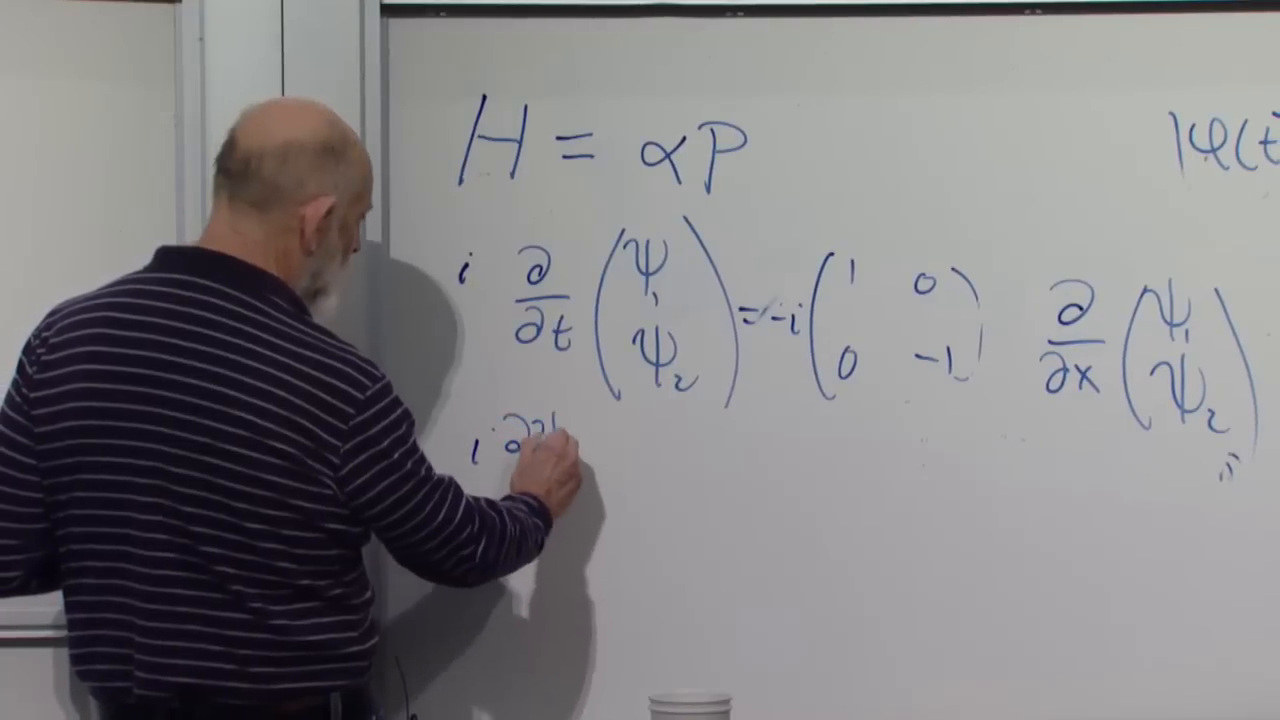
\includegraphics[width=0.94\linewidth]{lecture_09_frame_03.png}
\caption{La ecuación sin masa de dos componentes escrita en la pizarra: \(H=\alpha P\), con la matriz diagonal que asigna propagación en sentidos opuestos a \(\psi_1\) y \(\psi_2\).}
\lectureframe{01:26:00}
\end{figure}

El problema de la propagación en un solo sentido ha desaparecido. El espectro de energías negativas persiste, y hemos descubierto un tercer defecto: las dos componentes siguen siendo sin masa y se propagan a la velocidad de la luz. El siguiente paso debe introducir una energía en reposo y acoplar las dos direcciones.

\section{Añadir masa y descubrir el álgebra de Dirac}

Añadamos el término más general y sencillo proporcional a la masa:
\begin{equation}
H=\alpha p+\beta m,
\label{eq:l9-dirac-hamiltonian}
\end{equation}
donde \(\beta\) actúa solo sobre el índice de las dos componentes. Podría haber sido la identidad u otra matriz; dejaremos que la relación de dispersión relativista decida.

Como \(H^2\) debe ser igual a \(p^2+m^2\), elevemos al cuadrado la Ec.~\eqref{eq:l9-dirac-hamiltonian}:
\begin{align}
H^2
&=(\alpha p+\beta m)^2\\
&=\alpha^2p^2+\beta^2m^2
+(\alpha\beta+\beta\alpha)pm.
\label{eq:l9-square-dirac}
\end{align}
Las matrices conmutan con \(p\) porque actúan en el espacio interno de dos componentes, mientras que \(p\) actúa sobre la función de onda espacial. Para que concuerde con la Ec.~\eqref{eq:l9-rel-dispersion} se requiere
\begin{equation}
\alpha^2=\mathbb{1},
\qquad
\beta^2=\mathbb{1},
\qquad
\{\alpha,\beta\}
=\alpha\beta+\beta\alpha=0.
\label{eq:l9-dirac-algebra}
\end{equation}
La primera condición ya se cumple para \(\alpha=\sigma_3\). Cualquier otra matriz de Pauli anticonmuta con ella y su cuadrado es la identidad. Elijamos
\begin{equation}
\beta=
\begin{pmatrix}
0&1\\
1&0
\end{pmatrix}
=\sigma_1.
\label{eq:l9-beta}
\end{equation}
Elegir \(\sigma_1\) en lugar de \(\sigma_2\) es una convención de base; ambas realizan la misma álgebra tras un cambio unitario de base.

\begin{classroomqa}
\lecturetimestamp{01:33:00}
\audiencequestion{¿Dirac se limitó a reconocer que las matrices de Pauli satisfacen estas condiciones algebraicas?}
\lecturerresponse{La derivación histórica se llevó a cabo directamente en tres dimensiones e introdujo matrices que satisfacían las relaciones requeridas. Una vez escritas las condiciones, el álgebra de Pauli hace inmediata la solución unidimensional: basta elegir dos matrices de Pauli distintas.}
\end{classroomqa}

\begin{classroomqa}
\lecturetimestamp{01:34:24}
\audiencequestion{¿Es esta \(\beta\) el parámetro relativista de velocidad \(v/c\)?}
\lecturerresponse{No. Es una matriz que actúa sobre las componentes del espinor. La letra reutilizada es solo la notación de Dirac; no tiene nada que ver con la magnitud cinemática \(v/c\).}
\end{classroomqa}

En tres dimensiones espaciales, las matrices \(2\times2\) no bastan para formar el conjunto completo de matrices anticomutantes requerido. Dejaremos esa ampliación para más adelante. En una dimensión, las Ecs.~\eqref{eq:l9-alpha} y \eqref{eq:l9-beta} son suficientes.

\section{La ecuación de Dirac unidimensional acoplada}

Al sustituir \(p=-i\partial_x\), obtenemos la ecuación de Dirac unidimensional en forma hamiltoniana:
\begin{equation}
i\partial_t\Psi
=\left(-i\alpha\partial_x+\beta m\right)\Psi.
\label{eq:l9-one-dimensional-dirac}
\end{equation}
Como \(\alpha\) es diagonal, su término derivativo mantiene separadas las dos componentes. Como \(\beta\) es no diagonal, el término de masa las intercambia. Escrita componente a componente,
\begin{align}
i\partial_t\psi_1
&=-i\partial_x\psi_1+m\psi_2,
\label{eq:l9-dirac-component-one}\\
i\partial_t\psi_2
&=+i\partial_x\psi_2+m\psi_1.
\label{eq:l9-dirac-component-two}
\end{align}

\begin{figure}[htbp]
\centering
\includegraphics[width=0.94\linewidth]{lecture_09_frame_08.png}
\caption{Las ecuaciones acopladas para las componentes, escritas en la pizarra. Los signos opuestos de las derivadas codifican la propagación hacia la derecha y hacia la izquierda; el término de masa no diagonal intercambia \(\psi_1\) y \(\psi_2\).}
\lectureframe{01:37:44}
\end{figure}

Las componentes dejan de evolucionar independientemente en cuanto \(m\ne0\). Al elevar al cuadrado la ecuación de primer orden, se recupera el operador de Klein--Gordon en cada componente:
\begin{equation}
\left(\partial_t^2-\partial_x^2+m^2\right)\psi_a=0,
\qquad a=1,2,
\end{equation}
y las ondas planas satisfacen \(E^2=p^2+m^2\). Su velocidad de grupo es
\begin{equation}
v_g=\frac{dE}{dp}=\frac{p}{E},
\end{equation}
y su módulo es menor que uno si la masa no es nula.

La relación entre la masa y la mezcla de las componentes derecha e izquierda no es casual. Una partícula sin masa que se propaga hacia la derecha sigue haciéndolo bajo cualquier transformación de Lorentz propia: ningún observador sublumínico puede adelantarse a la luz e invertir su dirección. Una partícula masiva puede llevarse al reposo y luego observarse desde un sistema de referencia más rápido que se mueve en la misma dirección, en el que su velocidad parece invertirse. Por tanto, una teoría relativista con masa no puede mantener los sectores derecho e izquierdo permanentemente aislados. El término de masa no diagonal proporciona precisamente el acoplamiento requerido.

\begin{classroomqa}
\lecturetimestamp{01:40:01}
\audiencequestion{¿El intercambio entre las dos componentes es una oscilación quiral?}
\lecturerresponse{En esta base unidimensional, \(\alpha\) distingue las dos direcciones quirales sin masa. El término de masa es no diagonal y las mezcla, de modo que la quiralidad deja de conservarse. En ese sentido, el término de masa es el origen de la oscilación quiral.}
\end{classroomqa}

\begin{classroomqa}
\lecturetimestamp{01:40:46}
\audiencequestion{¿Por qué una ecuación para fermiones tendría que ser la raíz cuadrada de una ecuación para bosones?}
\lecturerresponse{No debe entenderse de ese modo. La relación de dispersión \(E^2=p^2+m^2\) se aplica a toda partícula relativista libre, independientemente de sus estadísticas. El operador de Dirac resulta proporcionar una factorización matricial del operador de Klein--Gordon, pero esa relación algebraica no deriva los fermiones de los bosones.}
\end{classroomqa}

\begin{classroomqa}
\lecturetimestamp{01:41:31}
\audiencequestion{¿Puede reducirse la ecuación a una factorización escalar sencilla en factores separados de propagación hacia la derecha y hacia la izquierda?}
\lecturerresponse{Solo en el límite sin masa se desacoplan las dos ecuaciones quirales en factores escalares independientes. Para \(m\ne0\), la factorización útil es matricial: las matrices anticomutantes \(\alpha\) y \(\beta\) son las que eliminan el término cruzado no deseado.}
\end{classroomqa}

\begin{classroomqa}
\lecturetimestamp{01:42:04}
\audiencequestion{¿Constituyen ya estas dos ecuaciones acopladas la ecuación de Dirac?}
\lecturerresponse{Sí. Juntas forman la ecuación de Dirac en una dimensión espacial, escrita de manera equivalente en la forma compacta de la Ec.~\eqref{eq:l9-one-dimensional-dirac}. Se puede obtener una notación covariante más simétrica multiplicando por \(\beta\), pero dejaremos esa forma para más adelante.}
\end{classroomqa}

Quedan deliberadamente sin resolver dos tareas. La construcción no ha eliminado las energías negativas; ha proporcionado soluciones de energía negativa en ambos sectores direccionales, por lo que el problema ahora se ve con mayor claridad, no con menor. Y la teoría sigue teniendo una sola dimensión espacial. Interpretar las soluciones de energía negativa y ampliar el álgebra de matrices a \(3+1\) dimensiones son los siguientes pasos.

\chapter{Fermiones, matrices de Dirac y mar de Dirac}

El mar de Dirac es nuestro destino, pero la ruta importa. Antes de abordar la energía negativa en la teoría relativista del electrón, necesitamos dos herramientas. Primero, el álgebra de operadores que distingue los fermiones de los bosones. Después, repasaremos la ecuación de Dirac unidimensional, donde cada ampliación de la función de onda puede verse sin la geometría de tres dimensiones espaciales. Con esas piezas ya dispuestas, la ecuación tridimensional impondrá su propia estructura matricial, y la discusión inicial de los estados fermiónicos ocupados y vacíos volverá a ser la clave para entender los positrones.

Usamos \(c=\hbar=1\). La letra mayúscula \(P\) denota un operador de momento; la minúscula \(p\), un autovalor del momento; y los símbolos en negrita, sus versiones tridimensionales.

\section{El intercambio se convierte en álgebra de operadores}

Consideremos dos partículas idénticas, una en \(x\) y otra en \(y\). Las etiquetas \(x\) y \(y\) denotan posiciones completas; no son dos coordenadas cartesianas de una sola partícula. Al actuar sobre el vacío con dos operadores de creación se obtiene
\begin{equation}
\lvert x,y\rangle
=
\psi^\dagger(x)\psi^\dagger(y)\lvert0\rangle.
\label{eq:l10-two-particle-state}
\end{equation}

Para los bosones, intercambiar las dos posiciones deja el estado inalterado:
\begin{equation}
\lvert x,y\rangle=\lvert y,x\rangle.
\end{equation}
La afirmación sobre los operadores que garantiza esta simetría es
\begin{equation}
\psi^\dagger(x)\psi^\dagger(y)
=
\psi^\dagger(y)\psi^\dagger(x).
\label{eq:l10-boson-exchange}
\end{equation}
Dos operadores de creación bosónicos conmutan, así que podemos invertir su orden sin cambiar el estado que crean.

Para los fermiones, el intercambio cambia el signo:
\begin{equation}
\lvert x,y\rangle=-\lvert y,x\rangle.
\label{eq:l10-fermion-state-exchange}
\end{equation}
El signo global de un vector de estado aislado no es observable, pero sí lo son los signos relativos entre alternativas, así que hay que conservar este signo menos de manera consistente. La ecuación~\eqref{eq:l10-fermion-state-exchange} exige
\begin{equation}
\psi^\dagger(x)\psi^\dagger(y)
=
-\,\psi^\dagger(y)\psi^\dagger(x).
\label{eq:l10-fermion-operator-exchange}
\end{equation}

\begin{figure}[htbp]
\centering
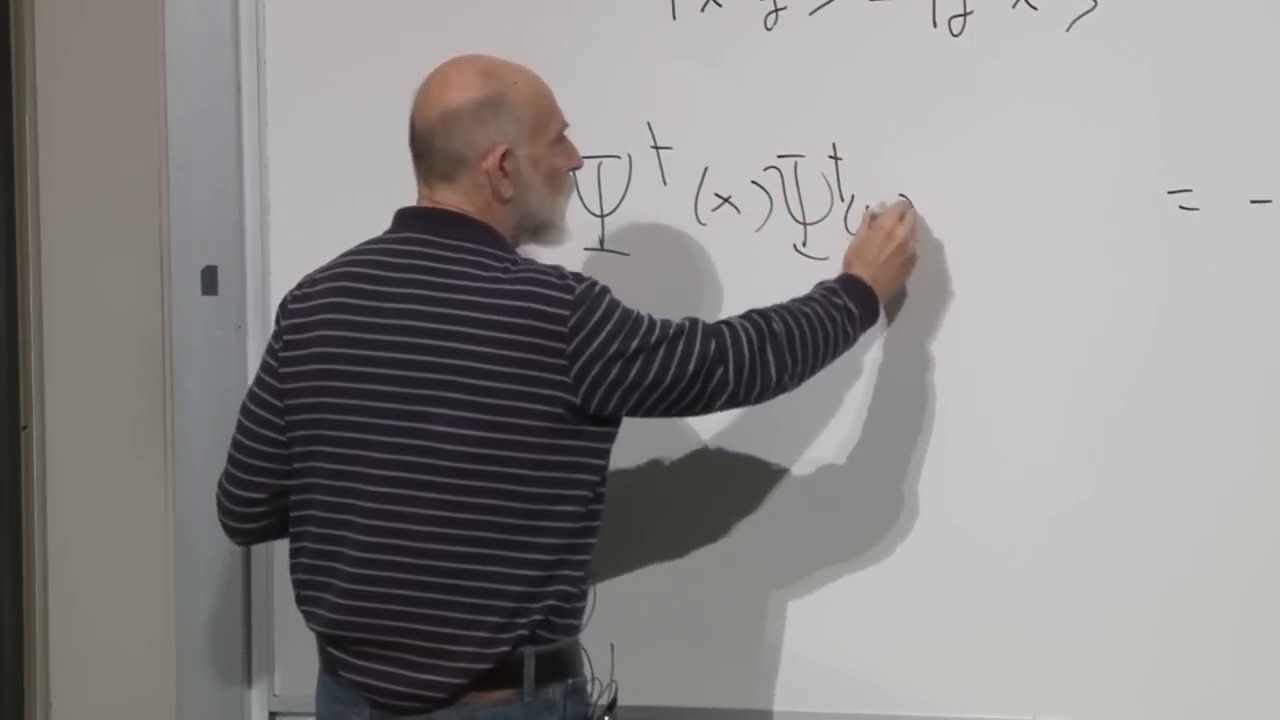
\includegraphics[width=0.94\linewidth]{lecture_10_figure_02.png}
\caption{La relación en la pizarra que implementa el intercambio fermiónico. Al intercambiar los operadores de creación, cambia el signo del estado de dos partículas.}
\lectureframe{00:05:50}
\end{figure}

Para dos operadores cualesquiera \(A\) y \(B\), definimos el anticonmutador como
\begin{equation}
\{A,B\}:=AB+BA.
\end{equation}
Por tanto, la regla de intercambio es
\begin{equation}
\{\psi^\dagger(x),\psi^\dagger(y)\}=0.
\label{eq:l10-creation-anticommutator}
\end{equation}
El álgebra correspondiente de los campos fermiónicos sustituye los conmutadores bosónicos por anticonmutadores. Hay que distinguir los dos usos de la palabra: los operadores de campo anticonmutan debido a la estadística de Fermi, mientras que más adelante las matrices anticonmutarán para cancelar términos cruzados en una relación de dispersión relativista.

Ahora tomemos \(y=x\) en la ecuación~\eqref{eq:l10-creation-anticommutator}. Ambos productos pasan a ser iguales:
\begin{align}
0
&=\{\psi^\dagger(x),\psi^\dagger(x)\}\\
&=2\,\psi^\dagger(x)\psi^\dagger(x).
\end{align}
Por tanto,
\begin{equation}
\bigl(\psi^\dagger(x)\bigr)^2=0.
\label{eq:l10-exclusion}
\end{equation}
Intentar crear dos fermiones idénticos en el mismo estado de una partícula da el vector nulo. Esta es la expresión en términos de operadores del principio de exclusión.

\begin{figure}[htbp]
\centering
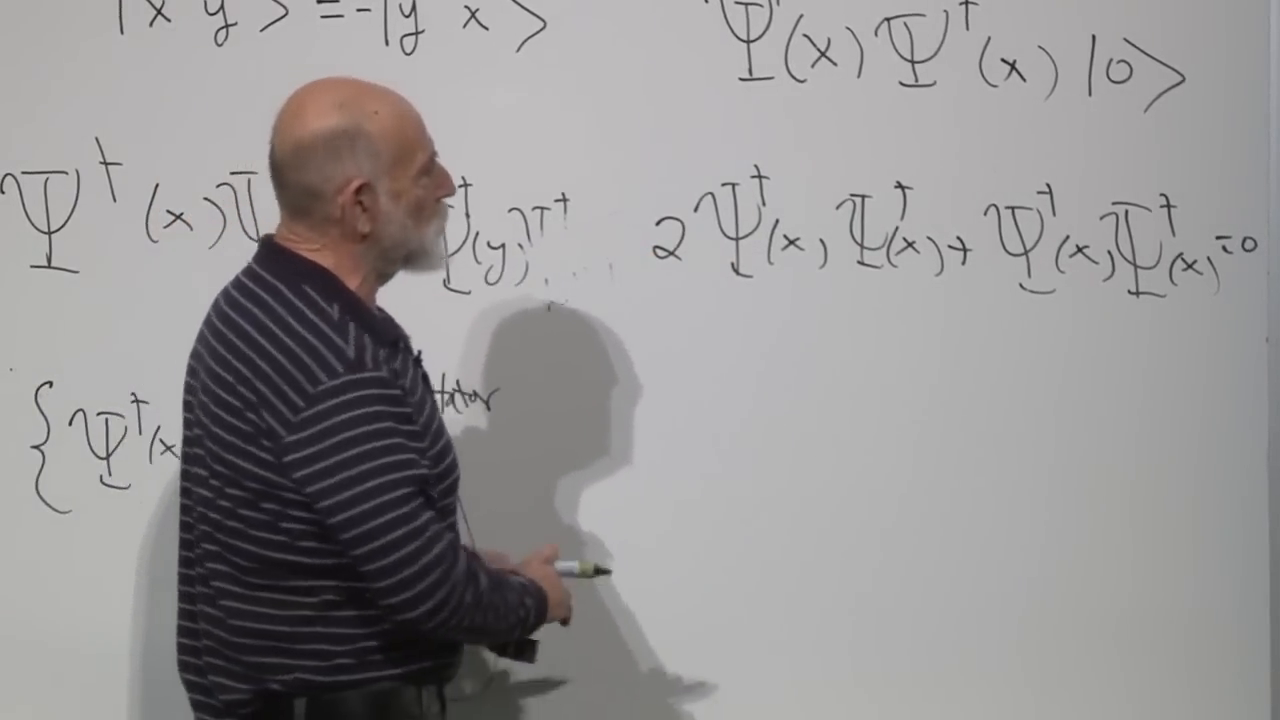
\includegraphics[width=0.94\linewidth]{lecture_10_figure_03.png}
\caption{El caso particular de estados iguales en la pizarra. El producto repetido de operadores de creación aparece dos veces y, por tanto, debe anularse.}
\lectureframe{00:08:04}
\end{figure}

\begin{figure}[htbp]
\centering
\begin{adjustbox}{max width=\linewidth}
\begin{tikzpicture}[node distance=1.25cm,>=Latex]
\node[draw,rounded corners,align=center,inner sep=7pt] (a)
  {$\{\psi^\dagger(x),\psi^\dagger(x)\}=0$};
\node[draw,rounded corners,align=center,inner sep=7pt,right=of a] (b)
  {$2(\psi^\dagger(x))^2=0$};
\node[draw,rounded corners,align=center,inner sep=7pt,right=of b] (c)
  {$(\psi^\dagger(x))^2=0$};
\draw[->,thick] (a) -- (b);
\draw[->,thick] (b) -- (c);
\end{tikzpicture}
\end{adjustbox}
\caption{La demostración de la exclusión, reconstruida sin el trabajo intermedio parcialmente borrado de la pizarra.}
\end{figure}

\section{Por qué para un fermión los estados ocupado y vacío son simétricos}

Hay una segunda diferencia entre los operadores bosónicos y fermiónicos, más sutil que la exclusión y esencial más adelante. Para un modo bosónico,
\begin{equation}
[a,a^\dagger]=1,
\qquad
n=0,1,2,\ldots.
\end{equation}
Intercambiar \(a\) y \(a^\dagger\) cambia el signo del conmutador. Aunque a los operadores se los llamara simplemente \(A\) y \(B\), el álgebra nos diría cuál de los órdenes aumenta el número de ocupación y cuál lo disminuye.

La escalera de ocupación bosónica también tiene una orientación. El operador de aniquilación acaba por llegar a \(\lvert0\rangle\) y da cero, mientras que el operador de creación puede continuar indefinidamente:
\begin{align}
a\lvert0\rangle&=0,\\
a^\dagger\lvert n\rangle&\propto\lvert n+1\rangle,
\qquad n=0,1,2,\ldots.
\end{align}
Invertir esta escalera no reproduce el mismo espectro. Hay un extremo inferior, pero no uno superior.

Para un modo fermiónico,
\begin{equation}
\{a,a^\dagger\}=1,
\qquad
a^2=(a^\dagger)^2=0,
\qquad
n=0,1.
\label{eq:l10-fermion-mode}
\end{equation}
El operador de creación lleva el estado vacío al estado ocupado y luego se detiene:
\begin{equation}
a^\dagger\lvert0\rangle=\lvert1\rangle,
\qquad
a^\dagger\lvert1\rangle=0.
\end{equation}
El operador de aniquilación hace lo contrario:
\begin{equation}
a\lvert1\rangle=\lvert0\rangle,
\qquad
a\lvert0\rangle=0.
\end{equation}
Solo hay dos estados, así que el diagrama es simétrico al intercambiar ocupado por vacío y \(a\) por \(a^\dagger\). Los operadores siguen teniendo significados físicos distintos, pero su álgebra ya no destaca uno como operador de creación y al otro como operador de aniquilación. Esta simetría formal es el germen de la reinterpretación en términos de partículas y huecos.

\begin{classroomqa}
\lecturetimestamp{00:13:54}
\audiencequestion{Si \((a^\dagger)^2=0\), ¿es una contradicción o implica que \(a^\dagger=0\)?}
\lecturerresponse{Ninguna de las dos cosas. Un operador no nulo puede tener cuadrado nulo. Aquí, \(a^\dagger\) lleva \(\lvert0\rangle\) a \(\lvert1\rangle\), pero no hay ningún estado permitido por encima de \(\lvert1\rangle\), así que aplicarlo dos veces da cero. El mismo razonamiento da \(a^2=0\).}
\end{classroomqa}

Tengamos presente esta simetría entre ocupado y vacío. Cuando se elimine un electrón de energía negativa, el operador de aniquilación se reinterpretará como operador de creación de positrones. No es un cambio arbitrario de notación: se apoya exactamente en el álgebra fermiónica de dos estados establecida aquí.

\section{La construcción de Dirac en una dimensión}

Volvamos ahora a una partícula en una dimensión espacial. La ecuación de onda relativista de primer orden más sencilla es
\begin{equation}
i\partial_t\psi=-\,i\partial_x\psi.
\label{eq:l10-right-mover}
\end{equation}
Con \(P=-i\partial_x\), queda
\begin{equation}
H=P.
\end{equation}
Un estado propio del momento tiene \(E=p\), y su velocidad de grupo es
\begin{equation}
v_g=\frac{dE}{dp}=1.
\end{equation}
Tanto el momento positivo como el negativo y, por tanto, tanto la energía positiva como la negativa dan lugar a una onda que se propaga rígidamente hacia la derecha. El signo de \(p\) cambia el patrón de fase, no el sentido de propagación.

Una partícula con masa debe poder moverse en cualquiera de los dos sentidos. Introduzcamos una segunda componente que satisfaga
\begin{equation}
H\psi_1=P\psi_1,
\qquad
H\psi_2=-P\psi_2.
\label{eq:l10-two-directions}
\end{equation}
La primera componente se propaga hacia la derecha; la segunda, hacia la izquierda. Reunámoslas en una columna,
\begin{equation}
\Psi=
\begin{pmatrix}
\psi_1\\
\psi_2
\end{pmatrix},
\end{equation}
y definamos
\begin{equation}
\alpha=
\begin{pmatrix}
1&0\\
0&-1
\end{pmatrix}.
\end{equation}
Ambas ecuaciones pasan a ser
\begin{equation}
H\Psi=\alpha P\Psi.
\label{eq:l10-massless-one-d}
\end{equation}
Incluir los dos sentidos tiene como coste un nuevo grado de libertad interno con dos valores.

La dirección por sí sola no produce la masa. Introduzcamos una segunda matriz,
\begin{equation}
\beta=
\begin{pmatrix}
0&1\\
1&0
\end{pmatrix},
\end{equation}
y probemos
\begin{equation}
H=\alpha P+\beta m.
\label{eq:l10-massive-one-d}
\end{equation}
Las matrices satisfacen
\begin{equation}
\alpha^2=\beta^2=\mathbb{1},
\qquad
\{\alpha,\beta\}=0.
\label{eq:l10-one-d-algebra}
\end{equation}
Al elevar el hamiltoniano al cuadrado se obtiene
\begin{align}
H^2
&=(\alpha P+\beta m)^2\\
&=\alpha^2P^2+\beta^2m^2
  +(\alpha\beta+\beta\alpha)Pm\\
&=P^2+m^2.
\label{eq:l10-one-d-dispersion}
\end{align}
El anticonmutador de la ecuación~\eqref{eq:l10-one-d-algebra} elimina el término no deseado que es lineal tanto en \(P\) como en \(m\).

La matriz no diagonal \(\beta\) acopla las dos componentes de dirección. Conviene imaginar el término de masa como una mezcla continua de las amplitudes que se propagan hacia la derecha y hacia la izquierda. No hay que tomar literalmente esta imagen como una partícula que rebota de un lado a otro por una trayectoria microscópica, pero sí ayuda a entender por qué un paquete de ondas masivo puede tener una velocidad media menor que la de la luz y un sistema de reposo, mientras que una componente quiral sin masa aislada no puede.

\begin{classroomqa}
\lecturetimestamp{00:23:37}
\audiencequestion{¿Hay una interpretación física más profunda de introducir ambas componentes de dirección?}
\lecturerresponse{Sí, pero se aprecia con más claridad en tres dimensiones. En esta etapa, son simplemente las dos componentes necesarias para describir propagaciones en sentidos opuestos y admitir un acoplamiento de masa no diagonal. Más adelante se interpretarán en términos de quiralidad, o helicidad.}
\end{classroomqa}

\section{Tres dimensiones exigen las matrices de Pauli}

En tres dimensiones espaciales, el momento es un vector. Un hamiltoniano lineal en el momento y escalar bajo rotaciones sugiere, por tanto, otro vector, esta vez un vector cuyas componentes son matrices:
\begin{equation}
H=\boldsymbol{\alpha}\cdot\mathbf P
=\alpha_xP_x+\alpha_yP_y+\alpha_zP_z.
\label{eq:l10-three-d-ansatz}
\end{equation}

\begin{figure}[htbp]
\centering
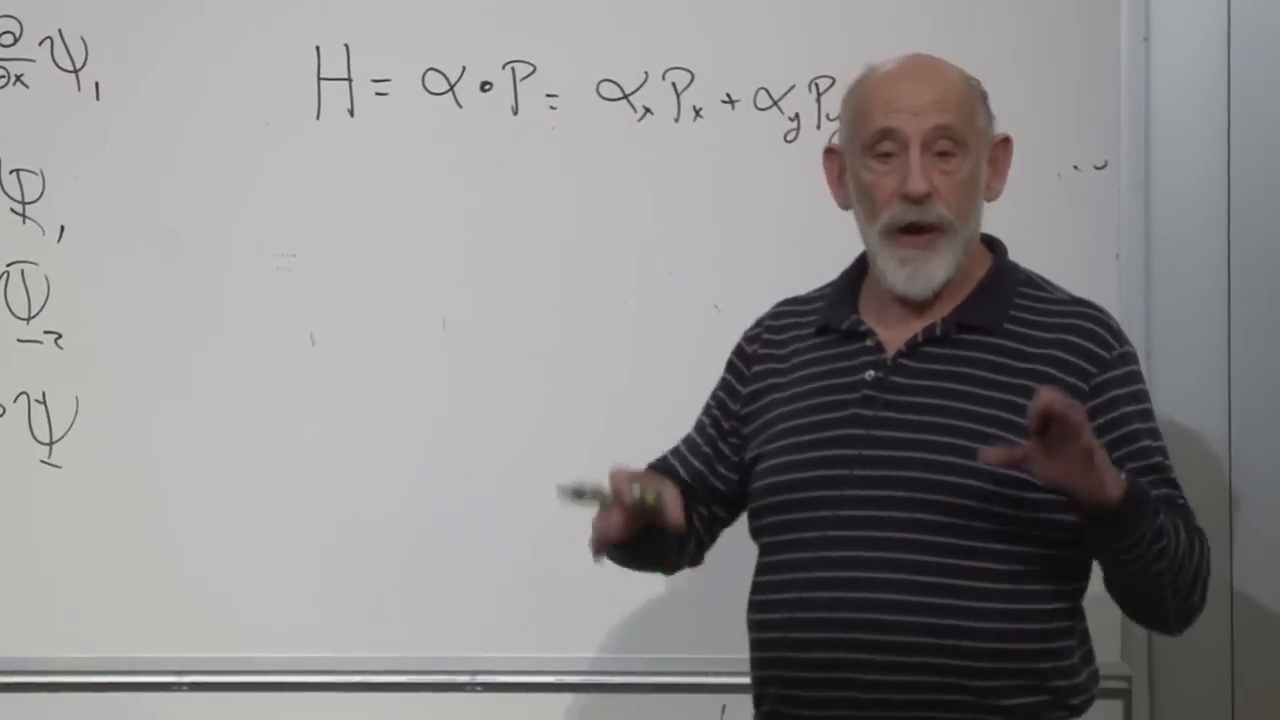
\includegraphics[width=0.94\linewidth]{lecture_10_figure_04.png}
\caption{El ansatz sin masa tridimensional \(H=\boldsymbol{\alpha}\cdot\mathbf P\) en el punto en que una matriz pasa a ser un vector de tres matrices.}
\lectureframe{00:26:00}
\end{figure}

Empecemos de nuevo con el caso sin masa. Exigimos
\begin{equation}
H^2=\mathbf P^2=P_x^2+P_y^2+P_z^2.
\end{equation}
Al desarrollar el cuadrado de la ecuación~\eqref{eq:l10-three-d-ansatz},
\begin{align}
H^2
&=\alpha_x^2P_x^2+\alpha_y^2P_y^2\\
&\quad+\alpha_z^2P_z^2\\
&\quad+\{\alpha_x,\alpha_y\}P_xP_y\\
&\quad+\{\alpha_x,\alpha_z\}P_xP_z\\
&\quad+\{\alpha_y,\alpha_z\}P_yP_z.
\end{align}
Los términos diagonales son los correctos si
\begin{equation}
\alpha_x^2=\alpha_y^2=\alpha_z^2=\mathbb{1},
\end{equation}
y todos los términos cruzados desaparecen si
\begin{equation}
\{\alpha_i,\alpha_j\}=0,
\qquad i\ne j.
\label{eq:l10-alpha-anticommutation}
\end{equation}

Tres matrices familiares \(2\times2\) hacen exactamente esto:
\begin{equation}
\sigma_x=
\begin{pmatrix}
0&1\\
1&0
\end{pmatrix},
\quad
\sigma_y=
\begin{pmatrix}
0&-i\\
i&0
\end{pmatrix},
\quad
\sigma_z=
\begin{pmatrix}
1&0\\
0&-1
\end{pmatrix}.
\label{eq:l10-pauli-matrices}
\end{equation}
Así, una solución es
\begin{equation}
\alpha_i=\sigma_i,
\qquad
H=\boldsymbol{\sigma}\cdot\mathbf P.
\label{eq:l10-weyl-hamiltonian}
\end{equation}

\begin{figure}[htbp]
\centering
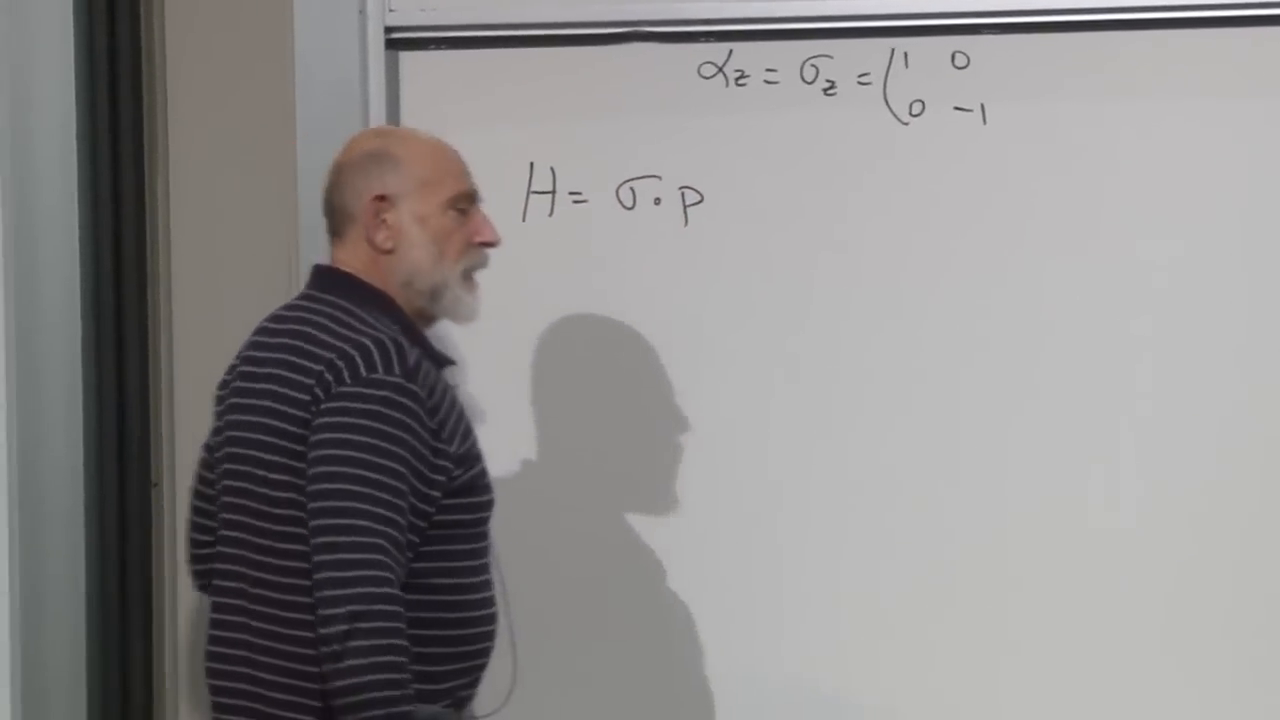
\includegraphics[width=0.94\linewidth]{lecture_10_figure_05.png}
\caption{El hamiltoniano sin masa en su forma compacta \(H=\boldsymbol{\sigma}\cdot\mathbf P\), con \(\alpha_z=\sigma_z\) aún visible encima.}
\lectureframe{00:28:16}
\end{figure}

Para un estado propio del momento,
\begin{equation}
\boldsymbol{\sigma}\cdot\mathbf p
=
|\mathbf p|\,\boldsymbol{\sigma}\cdot\widehat{\mathbf p}.
\end{equation}
El operador \(\boldsymbol{\sigma}\cdot\widehat{\mathbf p}\) tiene autovalores \(+1\) y \(-1\), así que
\begin{equation}
E=\pm|\mathbf p|.
\end{equation}
En esta teoría de dos componentes, para la energía positiva el grado de libertad de Pauli está alineado con el momento; para la energía negativa, está antialineado. La alineación está fijada: no es una dirección de espín que pueda ajustarse independientemente para un signo de energía dado.

\begin{classroomqa}
\lecturetimestamp{00:30:10}
\audiencequestion{¿El espín surge como consecuencia de la ecuación de Dirac o se introdujo porque ya se sabía que el electrón tiene momento magnético?}
\lecturerresponse{Aquí, «surgir» significa «aparecer como consecuencia», no «desaparecer». El punto de partida fue exigir un hamiltoniano lineal en el momento cuyo cuadrado fuera \(\mathbf P^2\). Los números ordinarios no pueden satisfacer el álgebra requerida, pero las matrices de Pauli sí. Por tanto, su estructura de dos componentes aparece con la propia linealización. Esto no demuestra que todas las partículas deban tener espín; indica que las partículas descritas por esta ecuación de tipo Dirac tienen el grado de libertad espinorial correspondiente.}
\end{classroomqa}

Esta es una de las lecciones centrales de la construcción. Las matrices no son etiquetas decorativas que se añaden después de encontrar la ecuación relativista. Surgen al intentar obtener una raíz cuadrada local de la relación de dispersión relativista.

\section{Por qué la masa requiere cuatro componentes}

Intentemos repetir la construcción unidimensional de la masa sin ampliar la teoría \(2\times2\):
\begin{equation}
H=\boldsymbol{\sigma}\cdot\mathbf P+\beta m.
\label{eq:l10-failed-mass}
\end{equation}
Supongamos que \(\beta^2=\mathbb{1}\). El cuadrado contiene los términos deseados \(\mathbf P^2+m^2\), pero también contiene
\begin{equation}
m\sum_i\{\sigma_i,\beta\}P_i.
\end{equation}
Para eliminar este término, una matriz \(\beta\) tendría que satisfacer
\begin{equation}
\{\sigma_x,\beta\}
=
\{\sigma_y,\beta\}
=
\{\sigma_z,\beta\}
=0.
\label{eq:l10-impossible-beta}
\end{equation}
Ninguna matriz \(2\times2\) lo hace. La identidad conmuta con las tres matrices de Pauli, y toda matriz \(2\times2\) sin traza es una combinación lineal de matrices de Pauli. Cualquier combinación así deja de anticonmutar con la componente paralela a ella. El álgebra \(2\times2\) no contiene una cuarta matriz independiente del tipo requerido.

La solución consiste en ampliar el espinor. Cuatro matrices que anticonmutan entre sí y cuyo cuadrado es la identidad aparecen por primera vez en una representación compleja \(4\times4\). Este tamaño matricial no se elige porque el espacio-tiempo tenga cuatro dimensiones; es el espacio matricial más pequeño capaz de realizar el álgebra requerida.

Hay muchas representaciones equivalentes. Un cambio unitario de base del espinor modifica las entradas de todas las matrices sin cambiar ninguna predicción física. Lo que importa es el conjunto abstracto de relaciones
\begin{equation}
\{\alpha_i,\alpha_j\}=2\delta_{ij}\mathbb{1},
\qquad
\{\alpha_i,\beta\}=0,
\qquad
\beta^2=\mathbb{1}.
\label{eq:l10-dirac-algebra}
\end{equation}

\begin{classroomqa}
\lecturetimestamp{00:37:38}
\audiencequestion{¿Puede considerarse \(\beta\) una componente temporal \(\alpha_t\)?}
\lecturerresponse{No directamente. Las tres \(\alpha_i\) no se combinan con \(\beta\) como las cuatro componentes de un solo vector de Lorentz. En notación covariante se definen, en cambio, \(\beta=\gamma^0\) y \(\alpha_i=\gamma^0\gamma^i\); las cuatro matrices \(\gamma^\mu\) satisfacen el álgebra de Clifford del espacio-tiempo.}
\end{classroomqa}

Una representación por bloques conveniente es
\begin{equation}
\alpha_i=
\begin{pmatrix}
\sigma_i&0\\
0&-\sigma_i
\end{pmatrix},
\qquad
\beta=
\begin{pmatrix}
0&I_2\\
I_2&0
\end{pmatrix}.
\label{eq:l10-block-representation}
\end{equation}
Las matrices de Pauli en los bloques diagonales garantizan que distintas \(\alpha_i\) anticonmuten. Los bloques de identidad no diagonales de \(\beta\) garantizan que \(\beta\) anticonmute con cada \(\alpha_i\).

\begin{figure}[htbp]
\centering
\includegraphics[width=0.94\linewidth]{lecture_10_figure_06.png}
\caption{La representación por bloques \(4\times4\) de la pizarra. Las ecuaciones superiores recogen los anticonmutadores requeridos; las matrices completas aparecen compuestas en la ecuación~\eqref{eq:l10-block-representation}.}
\lectureframe{00:41:10}
\end{figure}

Ahora el hamiltoniano con masa es
\begin{equation}
H=\boldsymbol{\alpha}\cdot\mathbf P+\beta m
=
\begin{pmatrix}
\boldsymbol{\sigma}\cdot\mathbf P&mI_2\\
mI_2&-\boldsymbol{\sigma}\cdot\mathbf P
\end{pmatrix}.
\label{eq:l10-massive-dirac}
\end{equation}
Usando la ecuación~\eqref{eq:l10-dirac-algebra},
\begin{equation}
H^2=\mathbf P^2+m^2.
\end{equation}
Por tanto, la estructura de cuatro componentes no es un añadido opcional. Es la estructura más pequeña que permite incluir tanto el momento tridimensional como un término de masa y mantener la ecuación de primer orden.

\section{La quiralidad y el significado de las componentes adicionales}

¿Qué distinción física aportó la ampliación? Empecemos con el bloque superior sin masa,
\begin{equation}
H_R=\boldsymbol{\sigma}\cdot\mathbf P,
\end{equation}
y el bloque inferior sin masa,
\begin{equation}
H_L=-\boldsymbol{\sigma}\cdot\mathbf P.
\end{equation}
En los estados de energía positiva, en el primero el espín está alineado con el momento y en el segundo está antialineado. Son helicidades opuestas. En una teoría sin masa, la helicidad es invariante bajo transformaciones de Lorentz propias, porque ningún observador puede sobrepasar a una partícula de tipo luz e invertir su momento sin dejar inalterado su espín. Por tanto, los dos bloques describen sectores quirales opuestos.

\begin{classroomqa}
\lecturetimestamp{00:41:28}
\audiencequestion{En una dimensión se necesitaba un grado de libertad binario adicional para introducir la masa. ¿Cuál es la distinción física correspondiente en tres dimensiones?}
\lecturerresponse{Es la quiralidad del espinor. Los dos bloques \(2\times2\) describen relaciones opuestas entre el espín y el momento. Uno es dextrógiro y el otro levógiro. La teoría \(4\times4\) contiene ambos.}
\end{classroomqa}

El término de masa en la ecuación~\eqref{eq:l10-massive-dirac} es no diagonal. Lleva una amplitud del bloque superior al inferior y viceversa:
\begin{equation}
\beta m
\begin{pmatrix}
\Psi_R\\
\Psi_L
\end{pmatrix}
=
m
\begin{pmatrix}
\Psi_L\\
\Psi_R
\end{pmatrix}.
\end{equation}
Por tanto, la masa acopla quiralidades opuestas.

\begin{classroomqa}
\lecturetimestamp{00:43:58}
\audiencequestion{¿Puede una partícula sin masa cambiar de quiralidad?}
\lecturerresponse{No en el hamiltoniano libre sin masa que se muestra aquí. Los dos bloques están desacoplados, así que un estado que comienza con quiralidad dextrógira o levógira la conserva. El término de masa no diagonal es precisamente lo que los mezcla cuando \(m\ne0\).}
\end{classroomqa}

Este lenguaje es exacto para la representación por bloques, pero no hay que llevar demasiado lejos la imagen de una partícula que alterna mecánicamente entre dos flechas. La afirmación física es el acoplamiento matricial en la ecuación de onda.

\begin{classroomqa}
\lecturetimestamp{00:44:50}
\audiencequestion{¿Están estas matrices incorporadas en los cuaterniones?}
\lecturerresponse{Las matrices de Pauli están estrechamente relacionadas con las unidades cuaterniónicas: las matrices \(-i\sigma_i\) al cuadrado dan \(-\mathbb{1}\) y se multiplican siguiendo el patrón cuaterniónico, salvo por las convenciones de orientación. Las matrices de Dirac completas requieren el álgebra de Clifford, más amplia, y la conexión con los cuaterniones no es necesaria para el argumento que sigue.}
\end{classroomqa}

\begin{classroomqa}
\lecturetimestamp{00:46:34}
\audiencequestion{Si el espín es momento angular, ¿hay aquí un término de energía independiente asociado a él?}
\lecturerresponse{No se añade ningún término independiente para la partícula libre. La estructura espinorial ya aparece en el hamiltoniano cinético a través de las matrices. Acoplar el espín a un campo magnético externo introduciría términos de interacción adicionales, pero ese es otro problema.}
\end{classroomqa}

\section{Las matrices alfa representan la velocidad, no el espín}

Cada \(\alpha_i\) tiene dos autovalores iguales a \(+1\) y dos iguales a \(-1\). Las distintas componentes no conmutan, así que no se pueden medir todas simultáneamente con precisión. Para identificar qué representa una de ellas, usemos la ecuación de Heisenberg. Para un operador \(L\) sin dependencia explícita del tiempo,
\begin{equation}
\dot L=i[H,L].
\label{eq:l10-heisenberg}
\end{equation}
La convención de signos queda fijada aquí por la evolución de Schr\"odinger \(e^{-iHt}\).

Apliquemos la ecuación~\eqref{eq:l10-heisenberg} al operador de posición \(x\). Las matrices actúan sobre los índices del espinor y conmutan con la posición, mientras que solo \(P_x\) no conmuta con \(x\):
\begin{align}
\dot x
&=i[\boldsymbol{\alpha}\cdot\mathbf P+\beta m,x]\\
&=i\alpha_x[P_x,x]\\
&=\alpha_x,
\label{eq:l10-velocity}
\end{align}
porque \([P_x,x]=-i\). Así, \(\alpha_x\) es la componente \(x\) del operador de velocidad; de manera análoga,
\begin{equation}
\dot{\mathbf x}=\boldsymbol{\alpha}.
\end{equation}

\begin{classroomqa}
\lecturetimestamp{00:51:50}
\audiencequestion{¿Una medición de una componente de la velocidad da realmente solo \(+1\) o \(-1\)?}
\lecturerresponse{Sí, para el operador instantáneo \(\alpha_i\) en unidades en las que \(c=1\). Un estado general no tiene por qué ser un estado propio, así que su valor esperado puede estar en cualquier punto entre esos valores. El paquete de ondas que se transporta suavemente tiene una velocidad media inferior a la de la luz cuando la partícula tiene masa.}
\end{classroomqa}

La velocidad no se conserva:
\begin{equation}
\dot\alpha_x=i[H,\alpha_x]\ne0.
\end{equation}
Los términos que contienen \(\alpha_y\), \(\alpha_z\) y \(\beta\) no conmutan con \(\alpha_x\). Por consiguiente, un estado que contenga componentes de energía tanto positiva como negativa presenta una contribución oscilatoria rápida a su posición. Esto es el \emph{zitterbewegung}, literalmente, movimiento tembloroso.

Tras promediar en tiempos largos comparados con la rápida oscilación, la velocidad relativista esperada es
\begin{equation}
\overline{\mathbf v}=\frac{\mathbf p}{E},
\end{equation}
que para un electrón lento se reduce a \(\mathbf p/m\).

\begin{classroomqa}
\lecturetimestamp{00:54:40}
\audiencequestion{¿Que un electrón libre tiemble sin fuerza externa contradice la ley de Newton?}
\lecturerresponse{No. La invariancia traslacional conserva el momento, de modo que \(\dot{\mathbf P}=0\). El operador de velocidad de Dirac no es simplemente \(\mathbf P/m\), y su parte rápidamente oscilatoria puede cambiar aunque el momento permanezca fijo. El movimiento promediado en el tiempo obedece la relación esperada para una partícula libre.}
\end{classroomqa}

\begin{classroomqa}
\lecturetimestamp{00:55:22}
\audiencequestion{¿La velocidad es siempre \(c\)?}
\lecturerresponse{Una medición instantánea de una componente \(\alpha_i\) tiene autovalores \(\pm c\), pero un paquete de ondas masivo es, en general, una superposición y tiene un valor esperado sublumínico. Su velocidad de grupo media es \(\mathbf p/E\).}
\end{classroomqa}

\begin{classroomqa}
\lecturetimestamp{00:55:30}
\audiencequestion{¿Se puede imaginar la oscilación como si la masa hiciera variar la velocidad?}
\lecturerresponse{No. La masa es un parámetro fijo. La oscilación se debe a que los operadores de velocidad y de hamiltoniano no conmutan o, equivalentemente, a la interferencia entre sectores de energía; no se debe a una masa fluctuante.}
\end{classroomqa}

\begin{classroomqa}
\lecturetimestamp{00:56:22}
\audiencequestion{¿Podría una medición instantánea encontrar la velocidad apuntando en un sentido aunque el movimiento medio apunte en otro?}
\lecturerresponse{Sí. El operador de la componente tiene los dos autovalores definidos, mientras que las mediciones repetidas o promediadas en el tiempo recuperan la deriva más suave.}
\end{classroomqa}

También hay que usar con cuidado la palabra espín. Las \(\alpha_i\) se transforman como componentes de la velocidad, que es un vector ordinario. El operador de espín propiamente dicho en esta representación es
\begin{equation}
\mathbf S=\frac12\boldsymbol{\Sigma},
\qquad
\Sigma_i=
\begin{pmatrix}
\sigma_i&0\\
0&\sigma_i
\end{pmatrix}.
\label{eq:l10-spin-operator}
\end{equation}
Difiere de \(\alpha_i\) en el signo del bloque inferior. Las matrices están estrechamente relacionadas, pero la velocidad y el espín no son el mismo observable.

\section{La energía negativa y el vacío de energía mínima}

El problema de la energía negativa ya estaba presente antes de introducir toda esta maquinaria matricial. Volvamos al modo que se propaga hacia la derecha en una dimensión,
\begin{equation}
H=P.
\end{equation}
Como \(p\) recorre toda la recta real, \(E=p\) no está acotada inferiormente.

El vacío no puede significar simplemente un estado sin partículas. Debe ser el estado al que ya no se le pueda extraer energía. Si un estado vacío permite añadir una partícula de energía negativa, reducir la energía, añadir otra y continuar indefinidamente, entonces ese estado no es un vacío estable.

La estadística de Fermi ofrece una salida histórica. Coloquemos un electrón en cada estado de energía negativa. Cada electrón añadido reduce la energía total, pero la exclusión permite un solo electrón en cada estado de una partícula. Una vez ocupados todos los estados de energía negativa, ningún electrón adicional puede caer en ese sector. Dirac identificó esta configuración llena como el vacío.

La misma construcción no funcionaría para los bosones. Se pueden ocupar con un número arbitrario de bosones un mismo estado, así que un modo bosónico de energía negativa podría absorber partículas sin límite. El límite fermiónico \(n=0,1\), introducido al comienzo de la clase, es precisamente lo que detiene el descenso.

\begin{figure}[htbp]
\centering
\includegraphics[width=0.94\linewidth]{lecture_10_figure_07.png}
\caption{La imagen histórica del mar de Dirac en la pizarra: una escalera de niveles de energía negativa llenos hasta la línea divisoria, con estados de energía positiva por encima.}
\lectureframe{01:02:45}
\end{figure}

\begin{figure}[htbp]
\centering
\begin{adjustbox}{max width=\linewidth}
\begin{tikzpicture}[x=1.05cm,y=0.72cm,>=Latex]
\draw[->] (0,-4.8) -- (0,4.8) node[above] {$E$};
\draw[thick] (-2.9,0) -- (3.2,0) node[right] {$E=0$};
\foreach \y in {-4,-3.3,...,-0.5} {
  \draw (-2.3,\y) -- (2.3,\y);
  \foreach \x in {-1.8,-1.2,...,1.8} {
    \fill[blue!65!black] (\x,\y) circle (1.6pt);
  }
}
\foreach \y in {0.8,1.6,...,4.0} {
  \draw (-2.3,\y) -- (2.3,\y);
}
\draw[red,very thick] (0.6,-2.6) circle (5pt);
\draw[red,->,very thick] (0.6,-2.35) .. controls (1.4,-0.4) and (1.2,1.6) .. (1.5,2.4);
\fill[red] (1.5,2.4) circle (2.5pt);
\node[right,red] at (0.85,-2.6) {hole};
\node[right,red] at (1.7,2.4) {$e^-$};
\node[left] at (-2.5,-2.2) {filled negative-energy states};
\end{tikzpicture}
\end{adjustbox}
\caption{Una reconstrucción clara de la excitación sobre un mar lleno: al promover un electrón de energía negativa queda un hueco de energía positiva.}
\end{figure}

La imagen del mar es una forma histórica de expresar una reordenación correcta de los operadores. No hay que confundir su carga y energía infinitas literales con magnitudes directamente observables; la reformulación moderna elimina la necesidad de imaginar electrones materiales que llenan el espacio.

\section{Un hueco es un positrón}

Con todos los estados de energía negativa ocupados, hay dos tipos posibles de excitación. Podemos añadir un electrón de energía positiva por encima del mar, o quitar un electrón de energía negativa y dejar un hueco.

El hueco tiene la carga opuesta a la del electrón que falta. Quitar una carga \(-e\) cambia la carga en \(+e\). También tiene energía de excitación positiva. Si el electrón eliminado tenía \(E_-<0\), la energía medida con respecto al vacío lleno cambia en
\begin{equation}
E_{\mathrm{hole}}=-E_->0.
\end{equation}
El hueco es una excitación de energía positiva y carga positiva: el positrón.

Un fotón puede promover un electrón del mar a un estado de energía positiva. Con respecto al vacío, el estado final contiene un electrón y un positrón. En un diagrama ordenado en el tiempo, se suele dibujar hacia arriba el flujo del número de electrones y, para la línea del positrón, la flecha en sentido opuesto. Las flechas indican el flujo del número fermiónico o de la carga; no son pequeños vectores clásicos de velocidad.

\begin{classroomqa}
\lecturetimestamp{01:05:14}
\audiencequestion{¿Esta imagen exige que haya igual número de electrones y positrones?}
\lecturerresponse{No en un estado arbitrario. Si partimos del vacío y creamos un par neutro, obtenemos uno de cada; pero un estado puede contener ya un exceso de electrones o de positrones. La conservación de la carga restringe las reacciones, pero no exige que todos los estados permitidos tengan poblaciones iguales.}
\end{classroomqa}

Al principio, Dirac no sabía que el hueco sería una partícula de masa idéntica a la del electrón y opuesta solo en carga y otros números cuánticos aditivos. La ecuación y la construcción del hueco condujeron a esa predicción antes de que el positrón se incorporara al catálogo familiar de partículas.

\section{Un solo campo fermiónico contiene electrones y positrones}

El operador de campo incorpora la imagen histórica al álgebra moderna. Por el momento, omitamos los índices espinoriales, los factores de normalización y la dependencia temporal. Un campo unidimensional puede desarrollarse esquemáticamente como
\begin{equation}
\psi(x)
\sim
\int_{-\infty}^{\infty}dp\,a(p)e^{ipx}.
\label{eq:l10-full-field-integral}
\end{equation}
Para la relación de dispersión de propagación a la derecha \(E=p\), un valor positivo de \(p\) indica energía positiva y uno negativo de \(p\), energía negativa. Separemos la integral:
\begin{equation}
\psi(x)
\sim
\int_0^\infty dp\,a(p)e^{ipx}
+
\int_{-\infty}^0 dp\,a(p)e^{ipx}.
\end{equation}
En el segundo término, hagamos el cambio \(p=-q\), con \(q>0\), y reinterpretemos la aniquilación de un electrón de energía negativa del mar lleno como creación de un positrón:
\begin{equation}
b^\dagger(q):=a(-q).
\end{equation}
Entonces
\begin{equation}
\psi(x)
\sim
\int_0^\infty dp\,
\left[
a(p)e^{ipx}
+
b^\dagger(p)e^{-ipx}
\right].
\label{eq:l10-electron-positron-split}
\end{equation}
Los signos exactos de las fases de las ondas planas dependen de la convención de espacio-tiempo; el contenido invariante es que \(\psi\) contiene un operador de aniquilación de electrones y uno de creación de positrones.

\begin{figure}[htbp]
\centering
\includegraphics[width=0.94\linewidth]{lecture_10_figure_08.png}
\caption{La integral del campo, separada en sectores de energía positiva y negativa. En la línea inferior se reetiqueta el operador del electrón de energía negativa como operador de creación de positrones.}
\lectureframe{01:11:35}
\end{figure}

Aquí entra en juego la simetría entre ocupado y vacío de la ecuación~\eqref{eq:l10-fermion-mode}. Para los fermiones, el álgebra de operadores permite esta reinterpretación sin cambiar la estructura de anticonmutación.

Una interacción electromagnética esquemática tiene la forma
\begin{equation}
H_{\mathrm{int}}
\sim
\int dx\,\psi^\dagger(x)\psi(x)A(x),
\label{eq:l10-qed-schematic}
\end{equation}
Aquí \(A\) denota el campo del fotón. Como cada campo fermiónico contiene partes de electrón y de positrón, un solo operador local contiene varios canales:
\begin{align}
e^-&\longrightarrow e^-+\gamma,\\
e^-+e^+&\longrightarrow\gamma,\\
\gamma&\longrightarrow e^-+e^+,
\end{align}
y también sus procesos inversos y cruzados. La conservación del momento y la energía determina qué canal es cinemáticamente posible en un entorno dado. Por ejemplo, un fotón real aislado en el vacío no puede crear un par sin otro participante que absorba el retroceso, aunque el vértice local esté presente en la interacción.

\begin{figure}[htbp]
\centering
\includegraphics[width=0.94\linewidth]{lecture_10_figure_09.png}
\caption{La pizarra reúne la emisión de un electrón, la aniquilación de un par y la interacción esquemática \(\psi^\dagger\psi A\). Al seleccionar distintas partes de los mismos operadores de campo se obtienen canales distintos.}
\lectureframe{01:13:30}
\end{figure}

Así, un producto compacto de campos organiza muchas reacciones que parecen diferentes. Más adelante, Feynman formuló las reglas diagramáticas sistemáticas para calcular las amplitudes, pero buena parte de la estructura de operadores ya se ve aquí.

\section{El lenguaje moderno del vacío y la analogía del mar de Fermi}

\begin{classroomqa}
\lecturetimestamp{01:14:20}
\audiencequestion{¿Cómo describen los físicos modernos esta situación sin tratar el vacío como un mar de Dirac literal?}
\lecturerresponse{Reinterpretan directamente los operadores. Se cambia el nombre del operador de aniquilación de electrones de energía negativa por el de operador de creación de positrones de energía positiva, y se define el vacío como el estado que anulan todos los operadores de aniquilación de electrones y positrones. La formulación resultante es simétrica entre partículas y antipartículas y no requiere ningún mar material.}
\end{classroomqa}

La imagen histórica del mar sigue siendo útil porque su lógica tiene un análogo cercano en la materia condensada. En un cristal, un número fijo de electrones ocupa los estados de una partícula de menor energía disponibles hasta el nivel de Fermi. El estado fundamental lleno no está vacío. Al promover un electrón por encima de ese nivel, queda un estado desocupado por debajo. Respecto del fondo lleno, el hueco tiene energía de excitación positiva y puede comportarse como un portador de carga positiva.

Hay diferencias importantes. Un hueco en un sólido existe en un medio, y su masa efectiva y su respuesta a la carga dependen de la estructura de bandas. Un positrón es una antipartícula elemental del campo cuántico relativista. Aun así, el álgebra común de partículas y huecos hace que la analogía sea poderosa.

\begin{classroomqa}
\lecturetimestamp{01:17:14}
\audiencequestion{¿La teoría de Klein--Gordon para bosones sufre la misma cascada hacia estados de energía negativa?}
\lecturerresponse{No. Un campo complejo de Klein--Gordon cuantizado correctamente se organiza en partículas y antipartículas de energía positiva, sin llenar un mar bosónico. Su ecuación de segundo orden y su estructura canónica difieren de la construcción del hamiltoniano de Dirac, así que el argumento histórico del mar fermiónico no se traslada sin cambios.}
\end{classroomqa}

\begin{classroomqa}
\lecturetimestamp{01:17:30}
\audiencequestion{¿De dónde proviene el espín uno de los bosones?}
\lecturerresponse{No de la linealización mediante matrices de Pauli que se usa aquí. Los campos de espín uno tienen su propia ley de transformación de Lorentz y sus propias ecuaciones de campo. La derivación presente explica la estructura espinorial de los fermiones de Dirac, no todos los espines posibles de las partículas.}
\end{classroomqa}

\begin{classroomqa}
\lecturetimestamp{01:17:46}
\audiencequestion{¿Por qué era esencial la estadística de Fermi para la solución de energía negativa?}
\lecturerresponse{Porque el principio de exclusión limita cada estado a un electrón. Una vez ocupados todos los estados de energía negativa, ningún otro electrón puede caer en ellos. La ocupación bosónica no tiene ese límite, así que un mar literal de bosones de energía negativa seguiría sin tener fondo.}
\end{classroomqa}

\begin{classroomqa}
\lecturetimestamp{01:20:02}
\audiencequestion{¿La distinción entre electrón y positrón es simplemente otro grado de libertad binario, como la carga?}
\lecturerresponse{Como recurso para contar estados, un campo de Dirac masivo tiene dos estados de espín del electrón y dos del positrón, así que dos etiquetas binarias son una regla mnemotécnica útil. Pero la distinción entre partícula y antipartícula no es un cúbit interno que pueda rotarse independientemente dentro de un electrón: todos los electrones tienen carga \(-e\), todos los positrones \(+e\), y la distinción surge de los sectores de frecuencia positiva y negativa tras la cuantización.}
\end{classroomqa}

El mar infinito plantea una última pregunta.

\begin{classroomqa}
\lecturetimestamp{01:20:54}
\audiencequestion{¿El mar infinito de Dirac produciría una constante cosmológica infinita?}
\lecturerresponse{Pone de manifiesto el problema de la energía del vacío. Los modos bosónicos de punto cero contribuyen \(+\tfrac12\hbar\omega\), mientras que los modos fermiónicos contribuyen con el signo opuesto. Son posibles cancelaciones formales cuando los espectros coinciden, pero los espectros del electrón y del fotón no coinciden, y cabe esperar un residuo enorme. Sin gravedad, se puede restar una constante al hamiltoniano porque solo importan las diferencias de energía. Con gravedad, la energía absoluta del vacío gravita, así que la sustracción se convierte en un problema físico y deja de ser una mera cuestión de contabilidad.}
\end{classroomqa}

La última vuelta nos lleva al significado de la masa.

\begin{classroomqa}
\lecturetimestamp{01:22:56}
\audiencequestion{¿Podemos decir algo más sobre cómo la masa relaciona las componentes levógira y dextrógira?}
\lecturerresponse{La afirmación exacta ya está en el hamiltoniano: el término no diagonal \(m\beta\) transforma un bloque quiral en el otro. Cualquier imagen más mecánica de un cambio microscópico entre ambos es opcional e inevitablemente incompleta.}
\end{classroomqa}
\end{document}